\definecolor{noteblu}{RGB}{60,60,180}
\definecolor{msgreen}{RGB}{0,140,60}
\definecolor{allocblue}{RGB}{100,160,220}

\tikzset{
  every node/.style={font=\scriptsize},
  inflow/.style={-{Latex[length=2.5mm]}, thick, green!60!black},
  outflow/.style={-{Latex[length=2.5mm]}, thick, red!70!black},
}

\newcommand{\BAC}{\mathrm{BAC}}
\newcommand{\EAC}{\mathrm{EAC}}

\section*{Test Verification Summary}
The table below shows pass (\checkmark), fail (\ding{55}), skip ($\circ$), or not-applicable (---) for each of the 11 test categories across all cases. Results are produced by \texttt{test\_milp.py} calling \texttt{baselines/milp.py}.

\begin{longtable}{lccccccccccc}
\toprule
\textbf{Case} & \rotatebox{70}{\scriptsize Budget alloc.} & \rotatebox{70}{\scriptsize Progress} & \rotatebox{70}{\scriptsize EVM signals} & \rotatebox{70}{\scriptsize Term.~counter} & \rotatebox{70}{\scriptsize MS cert.} & \rotatebox{70}{\scriptsize Payment id.} & \rotatebox{70}{\scriptsize Cash bal.} & \rotatebox{70}{\scriptsize $Z^*$} & \rotatebox{70}{\scriptsize Outcome} & \rotatebox{70}{\scriptsize P monotone} & \rotatebox{70}{\scriptsize Advance} \\
\midrule
\endfirsthead
\toprule
\textbf{Case} & \rotatebox{70}{\scriptsize Budget alloc.} & \rotatebox{70}{\scriptsize Progress} & \rotatebox{70}{\scriptsize EVM signals} & \rotatebox{70}{\scriptsize Term.~counter} & \rotatebox{70}{\scriptsize MS cert.} & \rotatebox{70}{\scriptsize Payment id.} & \rotatebox{70}{\scriptsize Cash bal.} & \rotatebox{70}{\scriptsize $Z^*$} & \rotatebox{70}{\scriptsize Outcome} & \rotatebox{70}{\scriptsize P monotone} & \rotatebox{70}{\scriptsize Advance} \\
\midrule
\endhead
\midrule \multicolumn{12}{r}{\small\itshape continued \ldots} \\
\endfoot
\bottomrule
\endlastfoot
\multicolumn{12}{l}{\small\textit{Group 1: Progress and Milestone Certification}} \\
\texttt{SP-1} & {\color{gray}---} & {\color{gray}---} & {\color{gray}---} & {\color{gray}---} & {\color{gray}---} & {\color{gray}---} & {\color{gray}---} & {\color{gray}---} & {\color{gray}---} & {\color{gray}---} & {\color{gray}---} \\
\texttt{SP-3} & {\color{gray}---} & {\color{gray}---} & {\color{gray}---} & {\color{gray}---} & {\color{gray}---} & {\color{gray}---} & {\color{gray}---} & {\color{gray}---} & {\color{gray}---} & {\color{gray}---} & {\color{gray}---} \\
\texttt{SP-J} & {\color{gray}---} & {\color{gray}---} & {\color{gray}---} & {\color{gray}---} & {\color{gray}---} & {\color{gray}---} & {\color{gray}---} & {\color{gray}---} & {\color{gray}---} & {\color{gray}---} & {\color{gray}---} \\
\multicolumn{12}{l}{\small\textit{Group 2: Discounting and Timing Incentives}} \\
\texttt{SP-4} & {\color{gray}---} & {\color{gray}---} & {\color{gray}---} & {\color{gray}---} & {\color{gray}---} & {\color{gray}---} & {\color{gray}---} & {\color{gray}---} & {\color{gray}---} & {\color{gray}---} & {\color{gray}---} \\
\texttt{MP-K} & {\color{gray}---} & {\color{gray}---} & {\color{gray}---} & {\color{gray}---} & {\color{gray}---} & {\color{gray}---} & {\color{gray}---} & {\color{gray}---} & {\color{gray}---} & {\color{gray}---} & {\color{gray}---} \\
\texttt{MP-Kp} & {\color{gray}---} & {\color{gray}---} & {\color{gray}---} & {\color{gray}---} & {\color{gray}---} & {\color{gray}---} & {\color{gray}---} & {\color{gray}---} & {\color{gray}---} & {\color{gray}---} & {\color{gray}---} \\
\texttt{SP-L} & {\color{gray}---} & {\color{gray}---} & {\color{gray}---} & {\color{gray}---} & {\color{gray}---} & {\color{gray}---} & {\color{gray}---} & {\color{gray}---} & {\color{gray}---} & {\color{gray}---} & {\color{gray}---} \\
\texttt{SP-Lp} & {\color{gray}---} & {\color{gray}---} & {\color{gray}---} & {\color{gray}---} & {\color{gray}---} & {\color{gray}---} & {\color{gray}---} & {\color{gray}---} & {\color{gray}---} & {\color{gray}---} & {\color{gray}---} \\
\texttt{SP-M} & {\color{gray}---} & {\color{gray}---} & {\color{gray}---} & {\color{gray}---} & {\color{gray}---} & {\color{gray}---} & {\color{gray}---} & {\color{gray}---} & {\color{gray}---} & {\color{gray}---} & {\color{gray}---} \\
\texttt{SP-Mp} & {\color{gray}---} & {\color{gray}---} & {\color{gray}---} & {\color{gray}---} & {\color{gray}---} & {\color{gray}---} & {\color{gray}---} & {\color{gray}---} & {\color{gray}---} & {\color{gray}---} & {\color{gray}---} \\
\multicolumn{12}{l}{\small\textit{Group 3: Advance Payments and Recovery}} \\
\texttt{SP-2} & {\color{gray}---} & {\color{gray}---} & {\color{gray}---} & {\color{gray}---} & {\color{gray}---} & {\color{gray}---} & {\color{gray}---} & {\color{gray}---} & {\color{gray}---} & {\color{gray}---} & {\color{gray}---} \\
\texttt{SP-2a} & {\color{gray}---} & {\color{gray}---} & {\color{gray}---} & {\color{gray}---} & {\color{gray}---} & {\color{gray}---} & {\color{gray}---} & {\color{gray}---} & {\color{gray}---} & {\color{gray}---} & {\color{gray}---} \\
\texttt{SP-2b} & {\color{gray}---} & {\color{gray}---} & {\color{gray}---} & {\color{gray}---} & {\color{gray}---} & {\color{gray}---} & {\color{gray}---} & {\color{gray}---} & {\color{gray}---} & {\color{gray}---} & {\color{gray}---} \\
\texttt{SP-2c} & {\color{gray}---} & {\color{gray}---} & {\color{gray}---} & {\color{gray}---} & {\color{gray}---} & {\color{gray}---} & {\color{gray}---} & {\color{gray}---} & {\color{gray}---} & {\color{gray}---} & {\color{gray}---} \\
\texttt{SP-2d} & {\color{gray}---} & {\color{gray}---} & {\color{gray}---} & {\color{gray}---} & {\color{gray}---} & {\color{gray}---} & {\color{gray}---} & {\color{gray}---} & {\color{gray}---} & {\color{gray}---} & {\color{gray}---} \\
\texttt{SP-A} & {\color{gray}---} & {\color{gray}---} & {\color{gray}---} & {\color{gray}---} & {\color{gray}---} & {\color{gray}---} & {\color{gray}---} & {\color{gray}---} & {\color{gray}---} & {\color{gray}---} & {\color{gray}---} \\
\texttt{SP-B} & {\color{gray}---} & {\color{gray}---} & {\color{gray}---} & {\color{gray}---} & {\color{gray}---} & {\color{gray}---} & {\color{gray}---} & {\color{gray}---} & {\color{gray}---} & {\color{gray}---} & {\color{gray}---} \\
\multicolumn{12}{l}{\small\textit{Group 4: Retention}} \\
\texttt{SP-C} & {\color{gray}---} & {\color{gray}---} & {\color{gray}---} & {\color{gray}---} & {\color{gray}---} & {\color{gray}---} & {\color{gray}---} & {\color{gray}---} & {\color{gray}---} & {\color{gray}---} & {\color{gray}---} \\
\texttt{SP-D} & {\color{gray}---} & {\color{gray}---} & {\color{gray}---} & {\color{gray}---} & {\color{gray}---} & {\color{gray}---} & {\color{gray}---} & {\color{gray}---} & {\color{gray}---} & {\color{gray}---} & {\color{gray}---} \\
\multicolumn{12}{l}{\small\textit{Group 5: Counter-Trajectory Cases (Active)}} \\
\texttt{SP-E} & {\color{gray}---} & {\color{gray}---} & {\color{gray}---} & {\color{gray}---} & {\color{gray}---} & {\color{gray}---} & {\color{gray}---} & {\color{gray}$\circ$} & {\color{gray}---} & {\color{gray}---} & {\color{gray}---} \\
\texttt{SP-F} & {\color{gray}---} & {\color{gray}---} & {\color{gray}---} & {\color{gray}---} & {\color{gray}---} & {\color{gray}---} & {\color{gray}---} & {\color{gray}$\circ$} & {\color{gray}---} & {\color{gray}---} & {\color{gray}---} \\
\texttt{SP-G} & {\color{gray}---} & {\color{gray}---} & {\color{gray}---} & {\color{gray}---} & {\color{gray}---} & {\color{gray}---} & {\color{gray}---} & {\color{gray}$\circ$} & {\color{gray}---} & {\color{gray}---} & {\color{gray}---} \\
\multicolumn{12}{l}{\small\textit{Group 6: Forced and Starvation Termination}} \\
\texttt{SP-5} & {\color{gray}---} & {\color{gray}---} & {\color{gray}---} & {\color{gray}---} & {\color{gray}---} & {\color{gray}---} & {\color{gray}---} & {\color{gray}---} & {\color{gray}---} & {\color{gray}---} & {\color{gray}---} \\
\texttt{SP-H} & {\color{gray}---} & {\color{gray}---} & {\color{gray}---} & {\color{gray}---} & {\color{gray}---} & {\color{gray}---} & {\color{gray}---} & {\color{gray}---} & {\color{gray}---} & {\color{gray}---} & {\color{gray}---} \\
\texttt{SP-I} & {\color{gray}---} & {\color{gray}---} & {\color{gray}---} & {\color{gray}---} & {\color{gray}---} & {\color{gray}---} & {\color{gray}---} & {\color{gray}$\circ$} & {\color{gray}---} & {\color{gray}---} & {\color{gray}---} \\
\multicolumn{12}{l}{\small\textit{Group 7: Multi-Project Mixed Outcomes}} \\
\texttt{MP-3} & {\color{gray}---} & {\color{gray}---} & {\color{gray}---} & {\color{gray}---} & {\color{gray}---} & {\color{gray}---} & {\color{gray}---} & {\color{gray}---} & {\color{gray}---} & {\color{gray}---} & {\color{gray}---} \\
\texttt{MP-A} & {\color{gray}---} & {\color{gray}---} & {\color{gray}---} & {\color{gray}---} & {\color{gray}---} & {\color{gray}---} & {\color{gray}---} & {\color{gray}---} & {\color{gray}---} & {\color{gray}---} & {\color{gray}---} \\
\texttt{MP-B} & {\color{gray}---} & {\color{gray}---} & {\color{gray}---} & {\color{gray}---} & {\color{gray}---} & {\color{gray}---} & {\color{gray}---} & {\color{gray}---} & {\color{gray}---} & {\color{gray}---} & {\color{gray}---} \\
\multicolumn{12}{l}{\small\textit{Group 8: Multi-Project Portfolio Optimisation}} \\
\texttt{MP-2} & {\color{gray}---} & {\color{gray}---} & {\color{gray}---} & {\color{gray}---} & {\color{gray}---} & {\color{gray}---} & {\color{gray}---} & {\color{gray}---} & {\color{gray}---} & {\color{gray}---} & {\color{gray}---} \\
\texttt{MP-4} & {\color{gray}---} & {\color{gray}---} & {\color{gray}---} & {\color{gray}---} & {\color{gray}---} & {\color{gray}---} & {\color{gray}---} & {\color{gray}---} & {\color{gray}---} & {\color{gray}---} & {\color{gray}---} \\
\texttt{MP-C} & {\color{gray}---} & {\color{gray}---} & {\color{gray}---} & {\color{gray}---} & {\color{gray}---} & {\color{gray}---} & {\color{gray}---} & {\color{gray}---} & {\color{gray}---} & {\color{gray}---} & {\color{gray}---} \\
\texttt{MP-D} & {\color{gray}---} & {\color{gray}---} & {\color{gray}---} & {\color{gray}---} & {\color{gray}---} & {\color{gray}---} & {\color{gray}---} & {\color{gray}---} & {\color{gray}---} & {\color{gray}---} & {\color{gray}---} \\
\multicolumn{12}{l}{\small\textit{Group 9: Staggered-Start Multi-Project}} \\
\texttt{MP-1} & {\color{gray}---} & {\color{gray}---} & {\color{gray}---} & {\color{gray}---} & {\color{gray}---} & {\color{gray}---} & {\color{gray}---} & {\color{gray}---} & {\color{gray}---} & {\color{gray}---} & {\color{gray}---} \\
\texttt{MP-E} & {\color{gray}---} & {\color{gray}---} & {\color{gray}---} & {\color{gray}---} & {\color{gray}---} & {\color{gray}---} & {\color{gray}---} & {\color{gray}---} & {\color{gray}---} & {\color{gray}---} & {\color{gray}---} \\
\end{longtable}

\newpage

\section*{Figure Legends}
All figures share the following visual language.
\medskip

\begin{tabular}{@{}p{4.5cm} p{9cm}@{}}
\toprule
\textbf{Panel} & \textbf{Meaning} \\
\midrule
\textbf{EVM (left)} &
  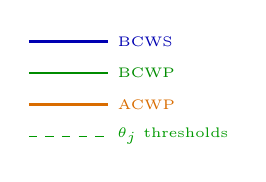
\begin{tikzpicture}[baseline=(current bounding box.center)]
    \draw[thick,blue!70!black]   (0,0)    -- (1,0)    node[right,font=\tiny]{BCWS};
    \draw[thick,green!55!black]  (0,-0.4) -- (1,-0.4) node[right,font=\tiny]{BCWP};
    \draw[thick,orange!85!black] (0,-0.8) -- (1,-0.8) node[right,font=\tiny]{ACWP};
    \draw[green!60!black,dashed,thin] (0,-1.2) -- (1,-1.2) node[right,font=\tiny]{$\theta_j$ thresholds};
  \end{tikzpicture} \\
\cmidrule{2-2}
& Red dashed vertical = termination period. \\
\midrule
\textbf{Profile (centre)} &
  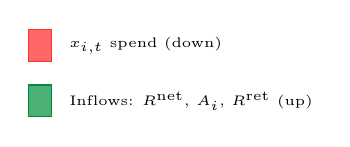
\begin{tikzpicture}[baseline=(current bounding box.center)]
    \draw[fill=red!60,draw=red!80] (0,0) rectangle (0.3,-0.4);
    \node[font=\tiny,anchor=west] at (0.4,-0.2) {$x_{i,t}$ spend (down)};
    \draw[fill=msgreen!70,draw=msgreen] (0,-0.7) rectangle (0.3,-1.1);
    \node[font=\tiny,anchor=west] at (0.4,-0.9) {Inflows: $R^{\mathrm{net}}$, $A_i$, $R^{\mathrm{ret}}$ (up)};
  \end{tikzpicture} \\
\midrule
\textbf{SPI/CPI (right)} &
  $\bullet$ = SPI (green),\quad $\blacksquare$ = CPI (orange),\quad
  red dashed = reference 1. \\
\midrule
\textbf{Portfolio left} &
  Cyan step-line = $B_t$; grey dashed = $B_1$ reference. \\
\midrule
\textbf{Portfolio centre} &
  Green bars = inflow, red bars = outflow,
  blue line with $\circ$ = net per period. \\
\midrule
\textbf{Portfolio right} &
  Blue line with $\bullet$ = cumulative discounted NCF. \\
\bottomrule
\end{tabular}

\bigskip
X-axes scale to each case's horizon $H$.
Middle project panel uses symmetric $\pm\BAC_i$ range.
Portfolio panels use data-driven ranges.

\newpage

\section*{Conventions}
\begin{itemize}
  \item $\gamma = 0.95$ throughout.
  \item Advance $A_i$ arrives at $t = s_i - 1$ (period~$0$ when $s_i=1$).
  \item Payment identity: $A_i + \sum_j R_{i,j}^{\mathrm{net}} + R_i^{\mathrm{ret}} = CP_i$
        checked for completed projects only.
  \item Retention released as a lump at the period the final milestone certifies.
  \item Advance recovery deductions: $\delta^{\mathrm{rec}} \phi_j CP_i$
        (pre-retention base, FIDIC convention).
\end{itemize}

\newpage

\section*{Cases}

\subsection*{Group 1: Progress and Milestone Certification}

\subsection*{SP-1  (Group~G1)}
\begin{center}
\begin{tabular}{ll}
\toprule
$n$,\;$H$ & $1$,\;$4$ \\
$\BAC,\;CP$ & $100,\;120$ \\
$s_i,\;f_i,\;D^{\mathrm{plan}}$ & $1,\;4,\;4$ \\
$\bar\eta$ & $1$ \\
$M,\;\theta$ & $2,\;(0.5,1)$ \\
$\phi,\;e_{i,j}$ & $(0.5,0.5),\;(1,3)$ \\
$\mu,\;\Omega,\;\tau^{\mathrm{tol}}$ & $0.3,\;1,\;2$ \\
$B_1,\;\gamma$ & $300,\;0.95$ \\
$Z^*$ & $19.025$ \\
Outcome & \texttt{completed} \\
\bottomrule
\end{tabular}
\end{center}

\begin{center}
\begin{tabular}{rrrrrrrrrrl}
\toprule
$t$ & $x$ & $P$ & BCWS & BCWP & ACWP & SPI & CPI & $\tau$ & MS & $R_{\mathrm{net}}$\\
\midrule
1 & 50 & 0.5 & 0.25 & 0.5 & 0.5 & 2 & 1 & 2 & \texttt{1} & 60 \\
2 & 0 & 0.5 & 0.5 & 0.5 & 0.5 & 1 & 1 & 2 & \texttt{---} & 0 \\
3 & 50 & 1 & 0.75 & 1 & 1 & 1.333 & 1 & 2 & \texttt{2} & 60 \\
4 & 0 & 1 & 1 & 1 & 1 & 1 & 1 & 2 & \texttt{---} & 0 \\
\bottomrule
\end{tabular}
\end{center}
\paragraph{Portfolio strip.}
\begin{center}
\begin{tabular}{rrrrrrr}
\toprule
$t$ & $B_t$ & $\Sigma\mathrm{In}$ & $\Sigma\mathrm{Out}$ & $\Sigma\mathrm{Net}$ & $\gamma^{t-1}\mathrm{Net}$ & $Z_t^{\mathrm{cum}}$\\
\midrule
1 & 310 & 60 & 50 & 10 & 10 & 10 \\
2 & 310 & 0 & 0 & 0 & 0 & 10 \\
3 & 320 & 60 & 50 & 10 & 9.025 & 19.025 \\
4 & 320 & 0 & 0 & 0 & 0 & 19.025 \\
\bottomrule
\end{tabular}
\end{center}

\begin{figure}[htbp]
\centering
% === Project 1 row for SP-1 ===
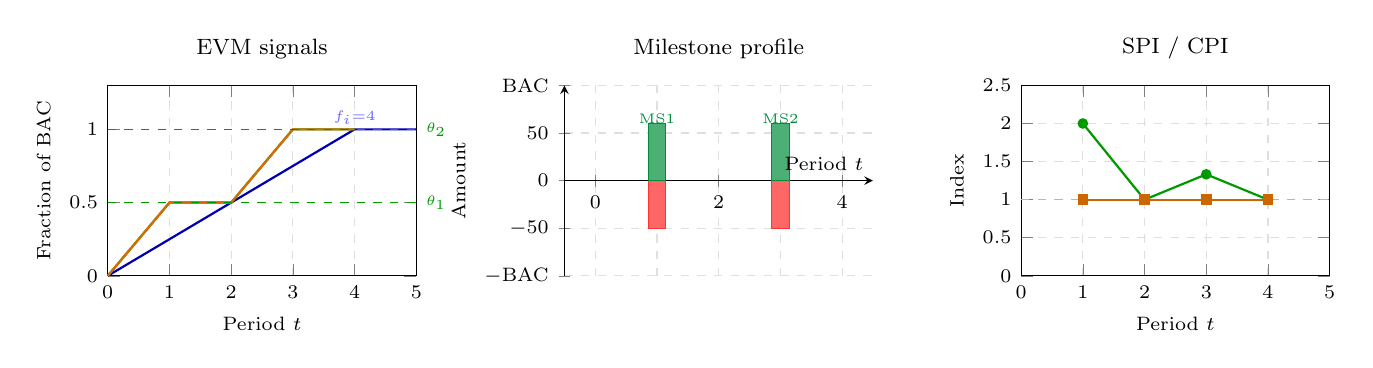
\begin{tikzpicture}[font=\footnotesize]
\begin{scope}
\begin{axis}[
    name=evmsp1_p1,
    width=5.5cm, height=4.0cm,
    title={\footnotesize EVM signals},
    xlabel={Period $t$}, ylabel={Fraction of $\BAC$},
    xmin=0, xmax=5, ymin=0, ymax=1.30,
    xtick={0,1,2,3,4,5},
    ytick={0,0.5,1},
    grid=major, grid style={dashed,gray!25},
    tick label style={font=\scriptsize},
    label style={font=\scriptsize}, title style={font=\scriptsize},
    clip=false,
  ]
  \addplot[thick,blue!70!black] coordinates {(0,0) (1,0.25) (2,0.5) (3,0.75) (4,1) (5,1)};
  \addplot[thick,green!55!black] coordinates {(0,0) (1,0.5) (2,0.5) (3,1) (4,1)};
  \addplot[thick,orange!85!black] coordinates {(0,0) (1,0.5) (2,0.5) (3,1) (4,1)};
  \draw[green!60!black,dashed,thin] (axis cs:0,0.5)--(axis cs:5,0.5) node[right,green!60!black,font=\tiny] {$\theta_{1}$};
  \draw[green!60!black,dashed,thin] (axis cs:0,1)--(axis cs:5,1) node[right,green!60!black,font=\tiny] {$\theta_{2}$};
  \node[font=\tiny,blue!60] at (axis cs:4,1.08) {$f_i{=}4$};
\end{axis}
\end{scope}

\begin{scope}[xshift=5.8cm]
\begin{axis}[
    name=mssp1_p1,
    width=5.5cm, height=4.0cm,
    title={\footnotesize Milestone profile},
    xlabel={Period $t$}, ylabel={Amount},
    xmin=-0.5, xmax=4.5, ymin=-100, ymax=100,
    xtick={0,1,2,3,4},
    ytick={-100,-50,0,50,100},
    yticklabels={$-\BAC$,$-50$,$0$,$50$,$\BAC$},
    grid=major, grid style={dashed,gray!25},
    tick label style={font=\scriptsize},
    label style={font=\scriptsize}, title style={font=\scriptsize},
    axis x line=center, axis y line=left,
    clip=false,
  ]
  \addplot[ybar,bar width=0.22cm,fill=red!60,draw=red!80] coordinates {(1,-50) (3,-50)};
  \addplot[ybar,bar width=0.22cm,fill=msgreen!70,draw=msgreen] coordinates {(1,60) (3,60)};
  \node[font=\tiny,msgreen] at (axis cs:1,65) {MS1};
  \node[font=\tiny,msgreen] at (axis cs:3,65) {MS2};
\end{axis}
\end{scope}

\begin{scope}[xshift=11.6cm]
\begin{axis}[
    name=spicpisp1_p1,
    width=5.5cm, height=4.0cm,
    title={\footnotesize SPI / CPI},
    xlabel={Period $t$}, ylabel={Index},
    xmin=0, xmax=5, ymin=0, ymax=2.5,
    xtick={0,1,2,3,4,5},
    ytick={0,0.5,1,1.5,2,2.5},
    grid=major, grid style={dashed,gray!25},
    tick label style={font=\scriptsize},
    label style={font=\scriptsize}, title style={font=\scriptsize},
    clip=false,
  ]
  \draw[red!40,dashed,thin] (axis cs:0,1)--(axis cs:5,1);
  \addplot[thick,green!60!black,mark=*,mark size=1.5pt] coordinates {(1,2) (2,1) (3,1.333) (4,1)};
  \addplot[thick,orange!80!black,mark=square*,mark size=1.5pt] coordinates {(1,1) (2,1) (3,1) (4,1)};
\end{axis}
\end{scope}

\end{tikzpicture}

\caption{SP-1 project view (single-project). Outcome: \texttt{completed}. $Z^*=19.025$.}
\label{fig:sp1_project}
\end{figure}

\begin{figure}[htbp]
\centering
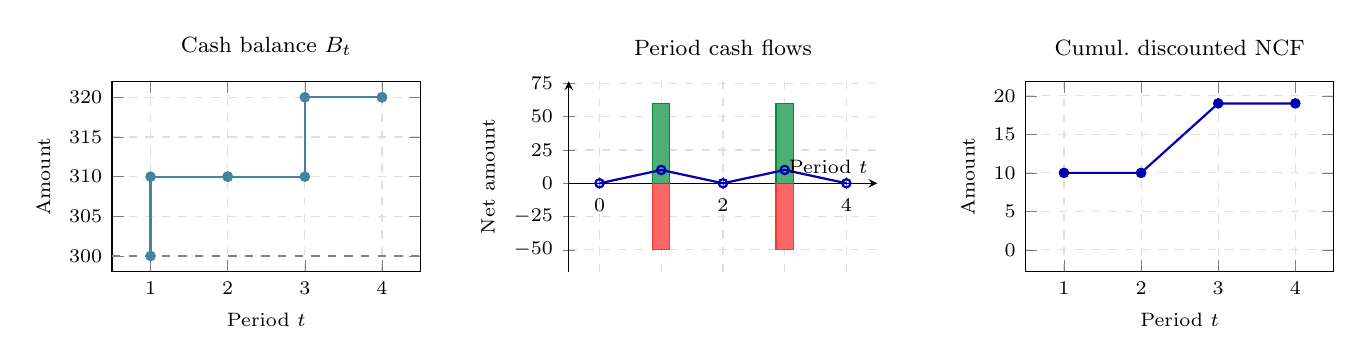
\begin{tikzpicture}[font=\footnotesize]
\begin{scope}
\begin{axis}[
    width=5.5cm, height=4.0cm,
    title={\footnotesize Cash balance $B_t$},
    xlabel={Period $t$}, ylabel={Amount},
    xmin=0.5, xmax=4.5,
    ymin=298, ymax=322,
    xtick={1,2,3,4},
    ytick={300,305,310,315,320},
    grid=major, grid style={dashed,gray!25},
    tick label style={font=\scriptsize},
    label style={font=\scriptsize}, title style={font=\scriptsize},
  ]
  \addplot[thick,cyan!60!black,mark=*,mark size=1.5pt] coordinates {(1,300) (1,310) (2,310) (2,310) (3,310) (3,320) (4,320) (4,320)};
  \draw[dashed,gray] (axis cs:0.5,300)--(axis cs:4.5,300) node[right,font=\tiny,gray] {$B_1$};
\end{axis}
\end{scope}

\begin{scope}[xshift=5.8cm]
\begin{axis}[
    width=5.5cm, height=4.0cm,
    title={\footnotesize Period cash flows},
    xlabel={Period $t$}, ylabel={Net amount},
    xmin=-0.5, xmax=4.5,
    ymin=-66.5, ymax=76.5,
    xtick={0,1,2,3,4},
    ytick={-50,-25,0,25,50,75},
    grid=major, grid style={dashed,gray!25},
    tick label style={font=\scriptsize},
    label style={font=\scriptsize}, title style={font=\scriptsize},
    axis x line=center, axis y line=left,
    clip=false,
  ]
  \addplot[ybar,bar width=0.22cm,fill=red!60,draw=red!80] coordinates {(1,-50) (3,-50)};
  \addplot[ybar,bar width=0.22cm,fill=msgreen!70,draw=msgreen] coordinates {(1,60) (3,60)};
  \addplot[thick,blue!70!black,mark=o,mark size=1.5pt] coordinates {(0,0) (1,10) (2,0) (3,10) (4,0)};
\end{axis}
\end{scope}

\begin{scope}[xshift=11.6cm]
\begin{axis}[
    width=5.5cm, height=4.0cm,
    title={\footnotesize Cumul.\ discounted NCF},
    xlabel={Period $t$}, ylabel={Amount},
    xmin=0.5, xmax=4.5,
    ymin=-2.854, ymax=21.879,
    xtick={1,2,3,4},
    ytick={0,5,10,15,20},
    grid=major, grid style={dashed,gray!25},
    tick label style={font=\scriptsize},
    label style={font=\scriptsize}, title style={font=\scriptsize},
  ]
  \addplot[thick,blue!70!black,mark=*,mark size=1.5pt] coordinates {(1,10) (2,10) (3,19.025) (4,19.025)};
\end{axis}
\end{scope}

\end{tikzpicture}
\caption{SP-1 portfolio view. $Z^*=19.025$.}
\label{fig:sp1_portfolio}
\end{figure}

\newpage

\subsection*{SP-3  (Group~G1)}
\begin{center}
\begin{tabular}{ll}
\toprule
$n$,\;$H$ & $1$,\;$6$ \\
$\BAC,\;CP$ & $60,\;90$ \\
$s_i,\;f_i,\;D^{\mathrm{plan}}$ & $1,\;6,\;6$ \\
$\bar\eta$ & $1$ \\
$M,\;\theta$ & $3,\;(0.333,0.667,1)$ \\
$\phi,\;e_{i,j}$ & $(0.333,0.333,0.333),\;(1,3,5)$ \\
$\mu,\;\Omega,\;\tau^{\mathrm{tol}}$ & $0.5,\;2,\;2$ \\
$B_1,\;\gamma$ & $300,\;0.95$ \\
$Z^*$ & $27.17$ \\
Outcome & \texttt{completed} \\
\bottomrule
\end{tabular}
\end{center}

\begin{center}
\begin{tabular}{rrrrrrrrrrl}
\toprule
$t$ & $x$ & $P$ & BCWS & BCWP & ACWP & SPI & CPI & $\tau$ & MS & $R_{\mathrm{net}}$\\
\midrule
1 & 20 & 0.333 & 0.167 & 0.333 & 0.333 & 2 & 1 & 2 & \texttt{1} & 30 \\
2 & 0 & 0.333 & 0.333 & 0.333 & 0.333 & 1 & 1 & 2 & \texttt{---} & 0 \\
3 & 20 & 0.667 & 0.5 & 0.667 & 0.667 & 1.333 & 1 & 2 & \texttt{2} & 30 \\
4 & 0 & 0.667 & 0.667 & 0.667 & 0.667 & 1 & 1 & 2 & \texttt{---} & 0 \\
5 & 20 & 1 & 0.833 & 1 & 1 & 1.2 & 1 & 2 & \texttt{3} & 30 \\
6 & 0 & 1 & 1 & 1 & 1 & 1 & 1 & 2 & \texttt{---} & 0 \\
\bottomrule
\end{tabular}
\end{center}
\paragraph{Portfolio strip.}
\begin{center}
\begin{tabular}{rrrrrrr}
\toprule
$t$ & $B_t$ & $\Sigma\mathrm{In}$ & $\Sigma\mathrm{Out}$ & $\Sigma\mathrm{Net}$ & $\gamma^{t-1}\mathrm{Net}$ & $Z_t^{\mathrm{cum}}$\\
\midrule
1 & 310 & 30 & 20 & 10 & 10 & 10 \\
2 & 310 & 0 & 0 & 0 & 0 & 10 \\
3 & 320 & 30 & 20 & 10 & 9.025 & 19.025 \\
4 & 320 & 0 & 0 & 0 & 0 & 19.025 \\
5 & 330 & 30 & 20 & 10 & 8.145 & 27.17 \\
6 & 330 & 0 & 0 & 0 & 0 & 27.17 \\
\bottomrule
\end{tabular}
\end{center}

\begin{figure}[htbp]
\centering
% === Project 1 row for SP-3 ===
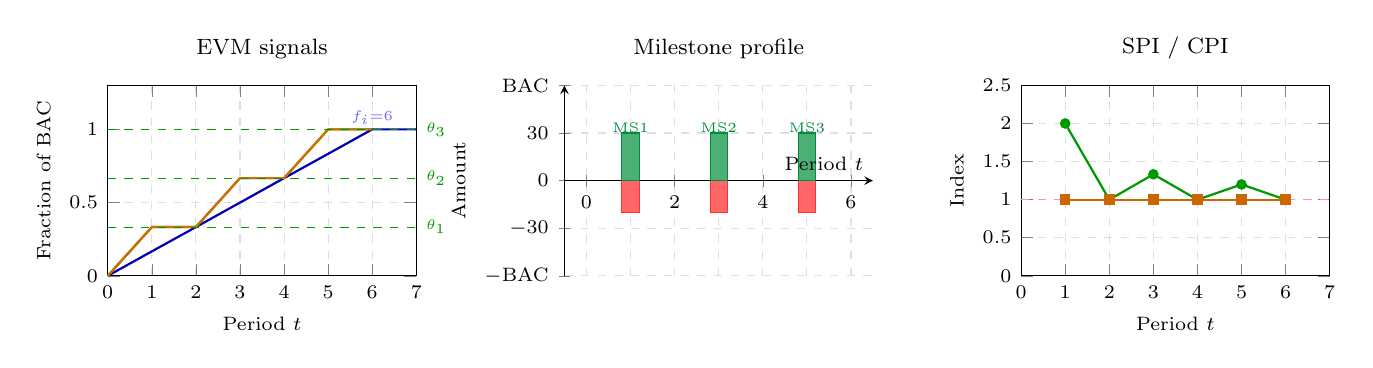
\begin{tikzpicture}[font=\footnotesize]
\begin{scope}
\begin{axis}[
    name=evmsp3_p1,
    width=5.5cm, height=4.0cm,
    title={\footnotesize EVM signals},
    xlabel={Period $t$}, ylabel={Fraction of $\BAC$},
    xmin=0, xmax=7, ymin=0, ymax=1.30,
    xtick={0,1,2,3,4,5,6,7},
    ytick={0,0.5,1},
    grid=major, grid style={dashed,gray!25},
    tick label style={font=\scriptsize},
    label style={font=\scriptsize}, title style={font=\scriptsize},
    clip=false,
  ]
  \addplot[thick,blue!70!black] coordinates {(0,0) (1,0.167) (2,0.333) (3,0.5) (4,0.667) (5,0.833) (6,1) (7,1)};
  \addplot[thick,green!55!black] coordinates {(0,0) (1,0.333) (2,0.333) (3,0.667) (4,0.667) (5,1) (6,1)};
  \addplot[thick,orange!85!black] coordinates {(0,0) (1,0.333) (2,0.333) (3,0.667) (4,0.667) (5,1) (6,1)};
  \draw[green!60!black,dashed,thin] (axis cs:0,0.333)--(axis cs:7,0.333) node[right,green!60!black,font=\tiny] {$\theta_{1}$};
  \draw[green!60!black,dashed,thin] (axis cs:0,0.667)--(axis cs:7,0.667) node[right,green!60!black,font=\tiny] {$\theta_{2}$};
  \draw[green!60!black,dashed,thin] (axis cs:0,1)--(axis cs:7,1) node[right,green!60!black,font=\tiny] {$\theta_{3}$};
  \node[font=\tiny,blue!60] at (axis cs:6,1.08) {$f_i{=}6$};
\end{axis}
\end{scope}

\begin{scope}[xshift=5.8cm]
\begin{axis}[
    name=mssp3_p1,
    width=5.5cm, height=4.0cm,
    title={\footnotesize Milestone profile},
    xlabel={Period $t$}, ylabel={Amount},
    xmin=-0.5, xmax=6.5, ymin=-60, ymax=60,
    xtick={0,1,2,3,4,5,6},
    ytick={-60,-30,0,30,60},
    yticklabels={$-\BAC$,$-30$,$0$,$30$,$\BAC$},
    grid=major, grid style={dashed,gray!25},
    tick label style={font=\scriptsize},
    label style={font=\scriptsize}, title style={font=\scriptsize},
    axis x line=center, axis y line=left,
    clip=false,
  ]
  \addplot[ybar,bar width=0.22cm,fill=red!60,draw=red!80] coordinates {(1,-20) (3,-20) (5,-20)};
  \addplot[ybar,bar width=0.22cm,fill=msgreen!70,draw=msgreen] coordinates {(1,30) (3,30) (5,30)};
  \node[font=\tiny,msgreen] at (axis cs:1,33) {MS1};
  \node[font=\tiny,msgreen] at (axis cs:3,33) {MS2};
  \node[font=\tiny,msgreen] at (axis cs:5,33) {MS3};
\end{axis}
\end{scope}

\begin{scope}[xshift=11.6cm]
\begin{axis}[
    name=spicpisp3_p1,
    width=5.5cm, height=4.0cm,
    title={\footnotesize SPI / CPI},
    xlabel={Period $t$}, ylabel={Index},
    xmin=0, xmax=7, ymin=0, ymax=2.5,
    xtick={0,1,2,3,4,5,6,7},
    ytick={0,0.5,1,1.5,2,2.5},
    grid=major, grid style={dashed,gray!25},
    tick label style={font=\scriptsize},
    label style={font=\scriptsize}, title style={font=\scriptsize},
    clip=false,
  ]
  \draw[red!40,dashed,thin] (axis cs:0,1)--(axis cs:7,1);
  \addplot[thick,green!60!black,mark=*,mark size=1.5pt] coordinates {(1,2) (2,1) (3,1.333) (4,1) (5,1.2) (6,1)};
  \addplot[thick,orange!80!black,mark=square*,mark size=1.5pt] coordinates {(1,1) (2,1) (3,1) (4,1) (5,1) (6,1)};
\end{axis}
\end{scope}

\end{tikzpicture}

\caption{SP-3 project view (single-project). Outcome: \texttt{completed}. $Z^*=27.17$.}
\label{fig:sp3_project}
\end{figure}

\begin{figure}[htbp]
\centering
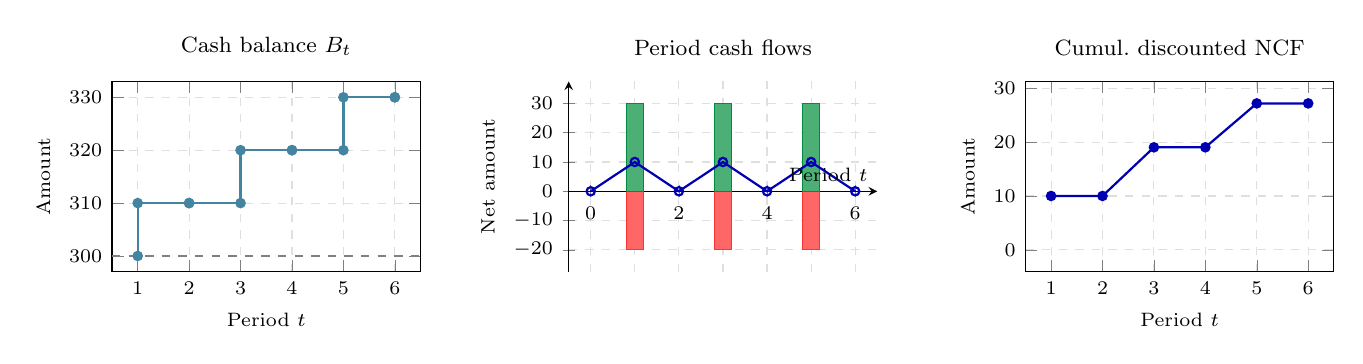
\begin{tikzpicture}[font=\footnotesize]
\begin{scope}
\begin{axis}[
    width=5.5cm, height=4.0cm,
    title={\footnotesize Cash balance $B_t$},
    xlabel={Period $t$}, ylabel={Amount},
    xmin=0.5, xmax=6.5,
    ymin=297, ymax=333,
    xtick={1,2,3,4,5,6},
    ytick={300,310,320,330},
    grid=major, grid style={dashed,gray!25},
    tick label style={font=\scriptsize},
    label style={font=\scriptsize}, title style={font=\scriptsize},
  ]
  \addplot[thick,cyan!60!black,mark=*,mark size=1.5pt] coordinates {(1,300) (1,310) (2,310) (2,310) (3,310) (3,320) (4,320) (4,320) (5,320) (5,330) (6,330) (6,330)};
  \draw[dashed,gray] (axis cs:0.5,300)--(axis cs:6.5,300) node[right,font=\tiny,gray] {$B_1$};
\end{axis}
\end{scope}

\begin{scope}[xshift=5.8cm]
\begin{axis}[
    width=5.5cm, height=4.0cm,
    title={\footnotesize Period cash flows},
    xlabel={Period $t$}, ylabel={Net amount},
    xmin=-0.5, xmax=6.5,
    ymin=-27.5, ymax=37.5,
    xtick={0,1,2,3,4,5,6},
    ytick={-20,-10,0,10,20,30},
    grid=major, grid style={dashed,gray!25},
    tick label style={font=\scriptsize},
    label style={font=\scriptsize}, title style={font=\scriptsize},
    axis x line=center, axis y line=left,
    clip=false,
  ]
  \addplot[ybar,bar width=0.22cm,fill=red!60,draw=red!80] coordinates {(1,-20) (3,-20) (5,-20)};
  \addplot[ybar,bar width=0.22cm,fill=msgreen!70,draw=msgreen] coordinates {(1,30) (3,30) (5,30)};
  \addplot[thick,blue!70!black,mark=o,mark size=1.5pt] coordinates {(0,0) (1,10) (2,0) (3,10) (4,0) (5,10) (6,0)};
\end{axis}
\end{scope}

\begin{scope}[xshift=11.6cm]
\begin{axis}[
    width=5.5cm, height=4.0cm,
    title={\footnotesize Cumul.\ discounted NCF},
    xlabel={Period $t$}, ylabel={Amount},
    xmin=0.5, xmax=6.5,
    ymin=-4.076, ymax=31.246,
    xtick={1,2,3,4,5,6},
    ytick={0,10,20,30},
    grid=major, grid style={dashed,gray!25},
    tick label style={font=\scriptsize},
    label style={font=\scriptsize}, title style={font=\scriptsize},
  ]
  \addplot[thick,blue!70!black,mark=*,mark size=1.5pt] coordinates {(1,10) (2,10) (3,19.025) (4,19.025) (5,27.17) (6,27.17)};
\end{axis}
\end{scope}

\end{tikzpicture}
\caption{SP-3 portfolio view. $Z^*=27.17$.}
\label{fig:sp3_portfolio}
\end{figure}

\newpage

\subsection*{SP-J  (Group~G1)}
\begin{center}
\begin{tabular}{ll}
\toprule
$n$,\;$H$ & $1$,\;$4$ \\
$\BAC,\;CP$ & $100,\;100$ \\
$s_i,\;f_i,\;D^{\mathrm{plan}}$ & $1,\;4,\;4$ \\
$\bar\eta$ & $1$ \\
$M,\;\theta$ & $2,\;(0.5,1)$ \\
$\phi,\;e_{i,j}$ & $(0.5,0.5),\;(1,3)$ \\
$\mu,\;\Omega,\;\tau^{\mathrm{tol}}$ & $0.5,\;2,\;2$ \\
$B_1,\;\gamma$ & $300,\;0.95$ \\
$Z^*$ & $0$ \\
Outcome & \texttt{completed} \\
\bottomrule
\end{tabular}
\end{center}

\begin{center}
\begin{tabular}{rrrrrrrrrrl}
\toprule
$t$ & $x$ & $P$ & BCWS & BCWP & ACWP & SPI & CPI & $\tau$ & MS & $R_{\mathrm{net}}$\\
\midrule
1 & 50 & 0.5 & 0.25 & 0.5 & 0.5 & 2 & 1 & 2 & \texttt{1} & 50 \\
2 & 0 & 0.5 & 0.5 & 0.5 & 0.5 & 1 & 1 & 2 & \texttt{---} & 0 \\
3 & 50 & 1 & 0.75 & 1 & 1 & 1.333 & 1 & 2 & \texttt{2} & 50 \\
4 & 0 & 1 & 1 & 1 & 1 & 1 & 1 & 2 & \texttt{---} & 0 \\
\bottomrule
\end{tabular}
\end{center}
\paragraph{Portfolio strip.}
\begin{center}
\begin{tabular}{rrrrrrr}
\toprule
$t$ & $B_t$ & $\Sigma\mathrm{In}$ & $\Sigma\mathrm{Out}$ & $\Sigma\mathrm{Net}$ & $\gamma^{t-1}\mathrm{Net}$ & $Z_t^{\mathrm{cum}}$\\
\midrule
1 & 300 & 50 & 50 & 0 & 0 & 0 \\
2 & 300 & 0 & 0 & 0 & 0 & 0 \\
3 & 300 & 50 & 50 & 0 & 0 & 0 \\
4 & 300 & 0 & 0 & 0 & 0 & 0 \\
\bottomrule
\end{tabular}
\end{center}

\begin{figure}[htbp]
\centering
% === Project 1 row for SP-J ===
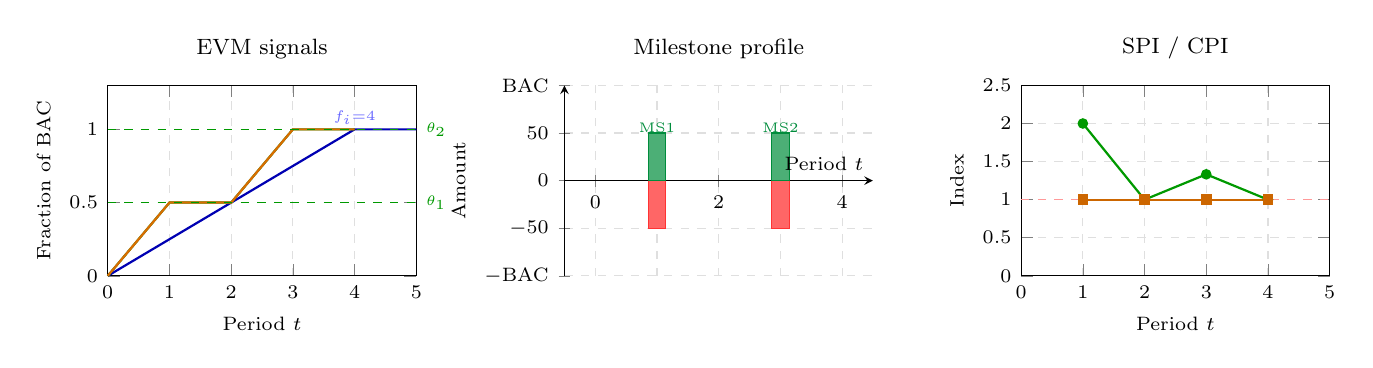
\begin{tikzpicture}[font=\footnotesize]
\begin{scope}
\begin{axis}[
    name=evmspj_p1,
    width=5.5cm, height=4.0cm,
    title={\footnotesize EVM signals},
    xlabel={Period $t$}, ylabel={Fraction of $\BAC$},
    xmin=0, xmax=5, ymin=0, ymax=1.30,
    xtick={0,1,2,3,4,5},
    ytick={0,0.5,1},
    grid=major, grid style={dashed,gray!25},
    tick label style={font=\scriptsize},
    label style={font=\scriptsize}, title style={font=\scriptsize},
    clip=false,
  ]
  \addplot[thick,blue!70!black] coordinates {(0,0) (1,0.25) (2,0.5) (3,0.75) (4,1) (5,1)};
  \addplot[thick,green!55!black] coordinates {(0,0) (1,0.5) (2,0.5) (3,1) (4,1)};
  \addplot[thick,orange!85!black] coordinates {(0,0) (1,0.5) (2,0.5) (3,1) (4,1)};
  \draw[green!60!black,dashed,thin] (axis cs:0,0.5)--(axis cs:5,0.5) node[right,green!60!black,font=\tiny] {$\theta_{1}$};
  \draw[green!60!black,dashed,thin] (axis cs:0,1)--(axis cs:5,1) node[right,green!60!black,font=\tiny] {$\theta_{2}$};
  \node[font=\tiny,blue!60] at (axis cs:4,1.08) {$f_i{=}4$};
\end{axis}
\end{scope}

\begin{scope}[xshift=5.8cm]
\begin{axis}[
    name=msspj_p1,
    width=5.5cm, height=4.0cm,
    title={\footnotesize Milestone profile},
    xlabel={Period $t$}, ylabel={Amount},
    xmin=-0.5, xmax=4.5, ymin=-100, ymax=100,
    xtick={0,1,2,3,4},
    ytick={-100,-50,0,50,100},
    yticklabels={$-\BAC$,$-50$,$0$,$50$,$\BAC$},
    grid=major, grid style={dashed,gray!25},
    tick label style={font=\scriptsize},
    label style={font=\scriptsize}, title style={font=\scriptsize},
    axis x line=center, axis y line=left,
    clip=false,
  ]
  \addplot[ybar,bar width=0.22cm,fill=red!60,draw=red!80] coordinates {(1,-50) (3,-50)};
  \addplot[ybar,bar width=0.22cm,fill=msgreen!70,draw=msgreen] coordinates {(1,50) (3,50)};
  \node[font=\tiny,msgreen] at (axis cs:1,55) {MS1};
  \node[font=\tiny,msgreen] at (axis cs:3,55) {MS2};
\end{axis}
\end{scope}

\begin{scope}[xshift=11.6cm]
\begin{axis}[
    name=spicpispj_p1,
    width=5.5cm, height=4.0cm,
    title={\footnotesize SPI / CPI},
    xlabel={Period $t$}, ylabel={Index},
    xmin=0, xmax=5, ymin=0, ymax=2.5,
    xtick={0,1,2,3,4,5},
    ytick={0,0.5,1,1.5,2,2.5},
    grid=major, grid style={dashed,gray!25},
    tick label style={font=\scriptsize},
    label style={font=\scriptsize}, title style={font=\scriptsize},
    clip=false,
  ]
  \draw[red!40,dashed,thin] (axis cs:0,1)--(axis cs:5,1);
  \addplot[thick,green!60!black,mark=*,mark size=1.5pt] coordinates {(1,2) (2,1) (3,1.333) (4,1)};
  \addplot[thick,orange!80!black,mark=square*,mark size=1.5pt] coordinates {(1,1) (2,1) (3,1) (4,1)};
\end{axis}
\end{scope}

\end{tikzpicture}

\caption{SP-J project view (single-project). Outcome: \texttt{completed}. $Z^*=0$.}
\label{fig:spj_project}
\end{figure}

\begin{figure}[htbp]
\centering
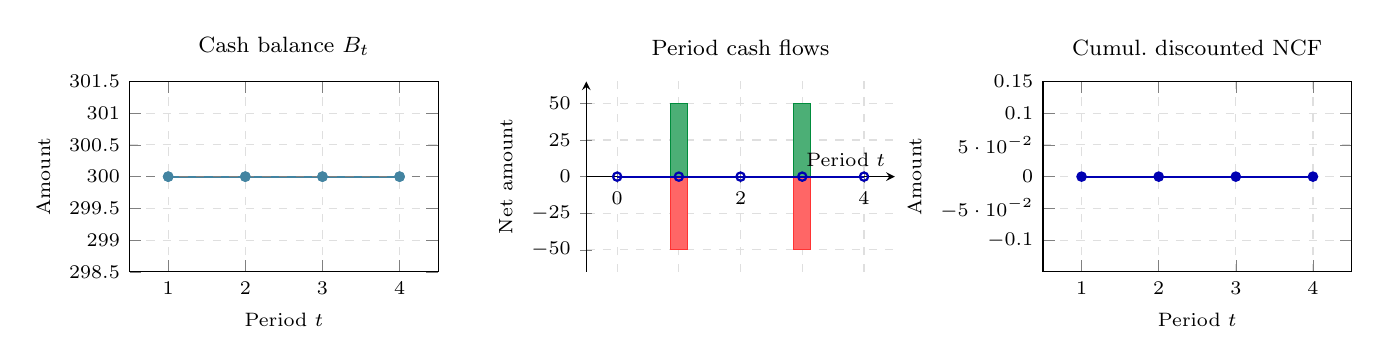
\begin{tikzpicture}[font=\footnotesize]
\begin{scope}
\begin{axis}[
    width=5.5cm, height=4.0cm,
    title={\footnotesize Cash balance $B_t$},
    xlabel={Period $t$}, ylabel={Amount},
    xmin=0.5, xmax=4.5,
    ymin=298.5, ymax=301.5,
    xtick={1,2,3,4},
    ytick={298.5,299,299.5,300,300.5,301,301.5},
    grid=major, grid style={dashed,gray!25},
    tick label style={font=\scriptsize},
    label style={font=\scriptsize}, title style={font=\scriptsize},
  ]
  \addplot[thick,cyan!60!black,mark=*,mark size=1.5pt] coordinates {(1,300) (1,300) (2,300) (2,300) (3,300) (3,300) (4,300) (4,300)};
  \draw[dashed,gray] (axis cs:0.5,300)--(axis cs:4.5,300) node[right,font=\tiny,gray] {$B_1$};
\end{axis}
\end{scope}

\begin{scope}[xshift=5.8cm]
\begin{axis}[
    width=5.5cm, height=4.0cm,
    title={\footnotesize Period cash flows},
    xlabel={Period $t$}, ylabel={Net amount},
    xmin=-0.5, xmax=4.5,
    ymin=-65, ymax=65,
    xtick={0,1,2,3,4},
    ytick={-50,-25,0,25,50},
    grid=major, grid style={dashed,gray!25},
    tick label style={font=\scriptsize},
    label style={font=\scriptsize}, title style={font=\scriptsize},
    axis x line=center, axis y line=left,
    clip=false,
  ]
  \addplot[ybar,bar width=0.22cm,fill=red!60,draw=red!80] coordinates {(1,-50) (3,-50)};
  \addplot[ybar,bar width=0.22cm,fill=msgreen!70,draw=msgreen] coordinates {(1,50) (3,50)};
  \addplot[thick,blue!70!black,mark=o,mark size=1.5pt] coordinates {(0,0) (1,0) (2,0) (3,0) (4,0)};
\end{axis}
\end{scope}

\begin{scope}[xshift=11.6cm]
\begin{axis}[
    width=5.5cm, height=4.0cm,
    title={\footnotesize Cumul.\ discounted NCF},
    xlabel={Period $t$}, ylabel={Amount},
    xmin=0.5, xmax=4.5,
    ymin=-0.15, ymax=0.15,
    xtick={1,2,3,4},
    ytick={-0.1,-0.05,0,0.05,0.1,0.15},
    grid=major, grid style={dashed,gray!25},
    tick label style={font=\scriptsize},
    label style={font=\scriptsize}, title style={font=\scriptsize},
  ]
  \addplot[thick,blue!70!black,mark=*,mark size=1.5pt] coordinates {(1,0) (2,0) (3,0) (4,0)};
\end{axis}
\end{scope}

\end{tikzpicture}
\caption{SP-J portfolio view. $Z^*=0$.}
\label{fig:spj_portfolio}
\end{figure}

\newpage


\subsection*{Group 2: Discounting and Timing Incentives}

\subsection*{SP-4  (Group~G2)}
\begin{center}
\begin{tabular}{ll}
\toprule
$n$,\;$H$ & $1$,\;$8$ \\
$\BAC,\;CP$ & $100,\;140$ \\
$s_i,\;f_i,\;D^{\mathrm{plan}}$ & $1,\;8,\;8$ \\
$\bar\eta$ & $1$ \\
$M,\;\theta$ & $2,\;(0.5,1)$ \\
$\phi,\;e_{i,j}$ & $(0.5,0.5),\;(1,5)$ \\
$\mu,\;\Omega,\;\tau^{\mathrm{tol}}$ & $0.3,\;1,\;2$ \\
$B_1,\;\gamma$ & $300,\;0.95$ \\
$Z^*$ & $36.29$ \\
Outcome & \texttt{completed} \\
\bottomrule
\end{tabular}
\end{center}

\begin{center}
\begin{tabular}{rrrrrrrrrrl}
\toprule
$t$ & $x$ & $P$ & BCWS & BCWP & ACWP & SPI & CPI & $\tau$ & MS & $R_{\mathrm{net}}$\\
\midrule
1 & 50 & 0.5 & 0.125 & 0.5 & 0.5 & 4 & 1 & 2 & \texttt{1} & 70 \\
2 & 0 & 0.5 & 0.25 & 0.5 & 0.5 & 2 & 1 & 2 & \texttt{---} & 0 \\
3 & 0 & 0.5 & 0.375 & 0.5 & 0.5 & 1.333 & 1 & 2 & \texttt{---} & 0 \\
4 & 0 & 0.5 & 0.5 & 0.5 & 0.5 & 1 & 1 & 2 & \texttt{---} & 0 \\
5 & 50 & 1 & 0.625 & 1 & 1 & 1.6 & 1 & 2 & \texttt{2} & 70 \\
6 & 0 & 1 & 0.75 & 1 & 1 & 1.333 & 1 & 2 & \texttt{---} & 0 \\
7 & 0 & 1 & 0.875 & 1 & 1 & 1.143 & 1 & 2 & \texttt{---} & 0 \\
8 & 0 & 1 & 1 & 1 & 1 & 1 & 1 & 2 & \texttt{---} & 0 \\
\bottomrule
\end{tabular}
\end{center}
\paragraph{Portfolio strip.}
\begin{center}
\begin{tabular}{rrrrrrr}
\toprule
$t$ & $B_t$ & $\Sigma\mathrm{In}$ & $\Sigma\mathrm{Out}$ & $\Sigma\mathrm{Net}$ & $\gamma^{t-1}\mathrm{Net}$ & $Z_t^{\mathrm{cum}}$\\
\midrule
1 & 320 & 70 & 50 & 20 & 20 & 20 \\
2 & 320 & 0 & 0 & 0 & 0 & 20 \\
3 & 320 & 0 & 0 & 0 & 0 & 20 \\
4 & 320 & 0 & 0 & 0 & 0 & 20 \\
5 & 340 & 70 & 50 & 20 & 16.29 & 36.29 \\
6 & 340 & 0 & 0 & 0 & 0 & 36.29 \\
7 & 340 & 0 & 0 & 0 & 0 & 36.29 \\
8 & 340 & 0 & 0 & 0 & 0 & 36.29 \\
\bottomrule
\end{tabular}
\end{center}

\begin{figure}[htbp]
\centering
% === Project 1 row for SP-4 ===
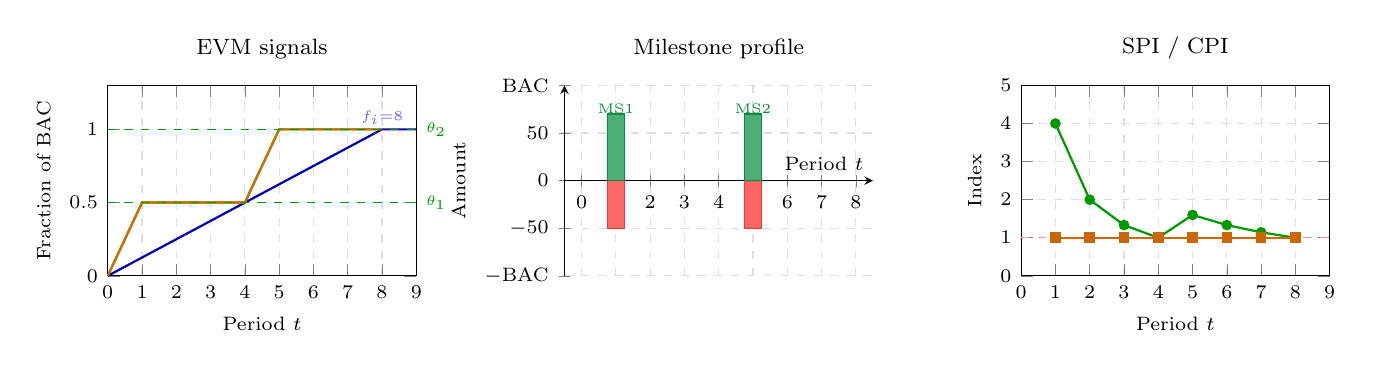
\begin{tikzpicture}[font=\footnotesize]
\begin{scope}
\begin{axis}[
    name=evmsp4_p1,
    width=5.5cm, height=4.0cm,
    title={\footnotesize EVM signals},
    xlabel={Period $t$}, ylabel={Fraction of $\BAC$},
    xmin=0, xmax=9, ymin=0, ymax=1.30,
    xtick={0,1,2,3,4,5,6,7,8,9},
    ytick={0,0.5,1},
    grid=major, grid style={dashed,gray!25},
    tick label style={font=\scriptsize},
    label style={font=\scriptsize}, title style={font=\scriptsize},
    clip=false,
  ]
  \addplot[thick,blue!70!black] coordinates {(0,0) (1,0.125) (2,0.25) (3,0.375) (4,0.5) (5,0.625) (6,0.75) (7,0.875) (8,1) (9,1)};
  \addplot[thick,green!55!black] coordinates {(0,0) (1,0.5) (2,0.5) (3,0.5) (4,0.5) (5,1) (6,1) (7,1) (8,1)};
  \addplot[thick,orange!85!black] coordinates {(0,0) (1,0.5) (2,0.5) (3,0.5) (4,0.5) (5,1) (6,1) (7,1) (8,1)};
  \draw[green!60!black,dashed,thin] (axis cs:0,0.5)--(axis cs:9,0.5) node[right,green!60!black,font=\tiny] {$\theta_{1}$};
  \draw[green!60!black,dashed,thin] (axis cs:0,1)--(axis cs:9,1) node[right,green!60!black,font=\tiny] {$\theta_{2}$};
  \node[font=\tiny,blue!60] at (axis cs:8,1.08) {$f_i{=}8$};
\end{axis}
\end{scope}

\begin{scope}[xshift=5.8cm]
\begin{axis}[
    name=mssp4_p1,
    width=5.5cm, height=4.0cm,
    title={\footnotesize Milestone profile},
    xlabel={Period $t$}, ylabel={Amount},
    xmin=-0.5, xmax=8.5, ymin=-100, ymax=100,
    xtick={0,1,2,3,4,5,6,7,8},
    ytick={-100,-50,0,50,100},
    yticklabels={$-\BAC$,$-50$,$0$,$50$,$\BAC$},
    grid=major, grid style={dashed,gray!25},
    tick label style={font=\scriptsize},
    label style={font=\scriptsize}, title style={font=\scriptsize},
    axis x line=center, axis y line=left,
    clip=false,
  ]
  \addplot[ybar,bar width=0.22cm,fill=red!60,draw=red!80] coordinates {(1,-50) (5,-50)};
  \addplot[ybar,bar width=0.22cm,fill=msgreen!70,draw=msgreen] coordinates {(1,70) (5,70)};
  \node[font=\tiny,msgreen] at (axis cs:1,75) {MS1};
  \node[font=\tiny,msgreen] at (axis cs:5,75) {MS2};
\end{axis}
\end{scope}

\begin{scope}[xshift=11.6cm]
\begin{axis}[
    name=spicpisp4_p1,
    width=5.5cm, height=4.0cm,
    title={\footnotesize SPI / CPI},
    xlabel={Period $t$}, ylabel={Index},
    xmin=0, xmax=9, ymin=0, ymax=5,
    xtick={0,1,2,3,4,5,6,7,8,9},
    ytick={0,1,2,3,4,5},
    grid=major, grid style={dashed,gray!25},
    tick label style={font=\scriptsize},
    label style={font=\scriptsize}, title style={font=\scriptsize},
    clip=false,
  ]
  \draw[red!40,dashed,thin] (axis cs:0,1)--(axis cs:9,1);
  \addplot[thick,green!60!black,mark=*,mark size=1.5pt] coordinates {(1,4) (2,2) (3,1.333) (4,1) (5,1.6) (6,1.333) (7,1.143) (8,1)};
  \addplot[thick,orange!80!black,mark=square*,mark size=1.5pt] coordinates {(1,1) (2,1) (3,1) (4,1) (5,1) (6,1) (7,1) (8,1)};
\end{axis}
\end{scope}

\end{tikzpicture}

\caption{SP-4 project view (single-project). Outcome: \texttt{completed}. $Z^*=36.29$.}
\label{fig:sp4_project}
\end{figure}

\begin{figure}[htbp]
\centering
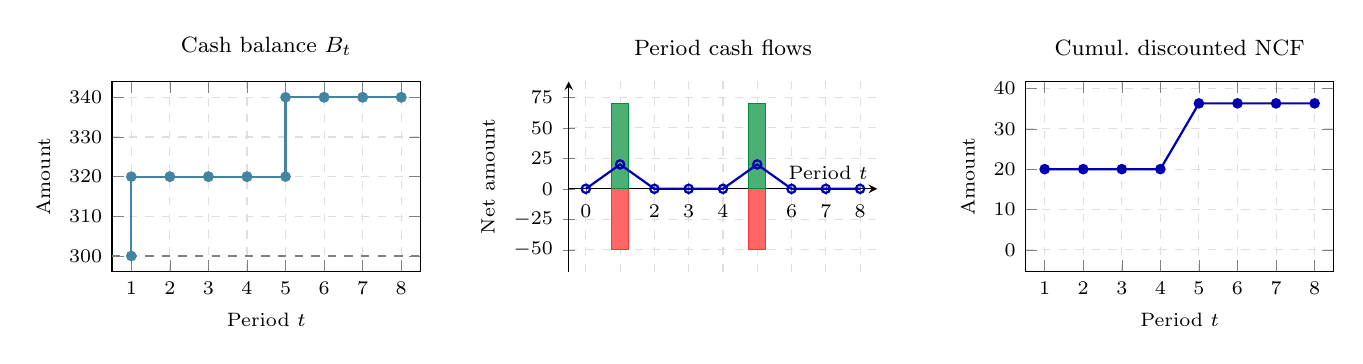
\begin{tikzpicture}[font=\footnotesize]
\begin{scope}
\begin{axis}[
    width=5.5cm, height=4.0cm,
    title={\footnotesize Cash balance $B_t$},
    xlabel={Period $t$}, ylabel={Amount},
    xmin=0.5, xmax=8.5,
    ymin=296, ymax=344,
    xtick={1,2,3,4,5,6,7,8},
    ytick={300,310,320,330,340},
    grid=major, grid style={dashed,gray!25},
    tick label style={font=\scriptsize},
    label style={font=\scriptsize}, title style={font=\scriptsize},
  ]
  \addplot[thick,cyan!60!black,mark=*,mark size=1.5pt] coordinates {(1,300) (1,320) (2,320) (2,320) (3,320) (3,320) (4,320) (4,320) (5,320) (5,340) (6,340) (6,340) (7,340) (7,340) (8,340) (8,340)};
  \draw[dashed,gray] (axis cs:0.5,300)--(axis cs:8.5,300) node[right,font=\tiny,gray] {$B_1$};
\end{axis}
\end{scope}

\begin{scope}[xshift=5.8cm]
\begin{axis}[
    width=5.5cm, height=4.0cm,
    title={\footnotesize Period cash flows},
    xlabel={Period $t$}, ylabel={Net amount},
    xmin=-0.5, xmax=8.5,
    ymin=-68, ymax=88,
    xtick={0,1,2,3,4,5,6,7,8},
    ytick={-50,-25,0,25,50,75},
    grid=major, grid style={dashed,gray!25},
    tick label style={font=\scriptsize},
    label style={font=\scriptsize}, title style={font=\scriptsize},
    axis x line=center, axis y line=left,
    clip=false,
  ]
  \addplot[ybar,bar width=0.22cm,fill=red!60,draw=red!80] coordinates {(1,-50) (5,-50)};
  \addplot[ybar,bar width=0.22cm,fill=msgreen!70,draw=msgreen] coordinates {(1,70) (5,70)};
  \addplot[thick,blue!70!black,mark=o,mark size=1.5pt] coordinates {(0,0) (1,20) (2,0) (3,0) (4,0) (5,20) (6,0) (7,0) (8,0)};
\end{axis}
\end{scope}

\begin{scope}[xshift=11.6cm]
\begin{axis}[
    width=5.5cm, height=4.0cm,
    title={\footnotesize Cumul.\ discounted NCF},
    xlabel={Period $t$}, ylabel={Amount},
    xmin=0.5, xmax=8.5,
    ymin=-5.444, ymax=41.734,
    xtick={1,2,3,4,5,6,7,8},
    ytick={0,10,20,30,40},
    grid=major, grid style={dashed,gray!25},
    tick label style={font=\scriptsize},
    label style={font=\scriptsize}, title style={font=\scriptsize},
  ]
  \addplot[thick,blue!70!black,mark=*,mark size=1.5pt] coordinates {(1,20) (2,20) (3,20) (4,20) (5,36.29) (6,36.29) (7,36.29) (8,36.29)};
\end{axis}
\end{scope}

\end{tikzpicture}
\caption{SP-4 portfolio view. $Z^*=36.29$.}
\label{fig:sp4_portfolio}
\end{figure}

\newpage

\subsection*{MP-K  (Group~G2)}
\begin{center}
\begin{tabular}{ll}
\toprule
$n$,\;$H$ & $2$,\;$6$ \\
$\BAC_i$ & $(60, 60)$ \\
$CP_i$   & $(90, 90)$ \\
$B_1,\;\gamma$ & $300,\;0.95$ \\
$Z^*$ & $55.87$ \\
Outcome & \texttt{both_completed} \\
\bottomrule
\end{tabular}
\end{center}

\paragraph{Project 1 timeline.}
\begin{center}
\begin{tabular}{rrrrrrrrrrl}
\toprule
$t$ & $x$ & $P$ & BCWS & BCWP & ACWP & SPI & CPI & $\tau$ & MS & $R_{\mathrm{net}}$\\
\midrule
1 & 30 & 0.5 & 0.167 & 0.5 & 0.5 & 3 & 1 & 2 & \texttt{1} & 63 \\
2 & 0 & 0.5 & 0.333 & 0.5 & 0.5 & 1.5 & 1 & 2 & \texttt{---} & 0 \\
3 & 0 & 0.5 & 0.5 & 0.5 & 0.5 & 1 & 1 & 2 & \texttt{---} & 0 \\
4 & 30 & 1 & 0.667 & 1 & 1 & 1.5 & 1 & 2 & \texttt{2} & 27 \\
5 & 0 & 1 & 0.833 & 1 & 1 & 1.2 & 1 & 2 & \texttt{---} & 0 \\
6 & 0 & 1 & 1 & 1 & 1 & 1 & 1 & 2 & \texttt{---} & 0 \\
\bottomrule
\end{tabular}
\end{center}
\paragraph{Project 2 timeline.}
\begin{center}
\begin{tabular}{rrrrrrrrrrl}
\toprule
$t$ & $x$ & $P$ & BCWS & BCWP & ACWP & SPI & CPI & $\tau$ & MS & $R_{\mathrm{net}}$\\
\midrule
1 & 0 & 0 & 0.167 & 0 & 0 & 0 & 1 & 2 & \texttt{---} & 0 \\
2 & 30 & 0.5 & 0.333 & 0.5 & 0.5 & 1.5 & 1 & 2 & \texttt{1} & 27 \\
3 & 0 & 0.5 & 0.5 & 0.5 & 0.5 & 1 & 1 & 2 & \texttt{---} & 0 \\
4 & 30 & 1 & 0.667 & 1 & 1 & 1.5 & 1 & 2 & \texttt{2} & 63 \\
5 & 0 & 1 & 0.833 & 1 & 1 & 1.2 & 1 & 2 & \texttt{---} & 0 \\
6 & 0 & 1 & 1 & 1 & 1 & 1 & 1 & 2 & \texttt{---} & 0 \\
\bottomrule
\end{tabular}
\end{center}
\paragraph{Portfolio strip.}
\begin{center}
\begin{tabular}{rrrrrrr}
\toprule
$t$ & $B_t$ & $\Sigma\mathrm{In}$ & $\Sigma\mathrm{Out}$ & $\Sigma\mathrm{Net}$ & $\gamma^{t-1}\mathrm{Net}$ & $Z_t^{\mathrm{cum}}$\\
\midrule
1 & 333 & 63 & 30 & 33 & 33 & 33 \\
2 & 330 & 27 & 30 & -3 & -2.85 & 30.15 \\
3 & 330 & 0 & 0 & 0 & 0 & 30.15 \\
4 & 360 & 90 & 60 & 30 & 25.721 & 55.871 \\
5 & 360 & 0 & 0 & 0 & 0 & 55.871 \\
6 & 360 & 0 & 0 & 0 & 0 & 55.871 \\
\bottomrule
\end{tabular}
\end{center}

\begin{figure}[htbp]
\centering
% === Project 1 row for MP-K ===
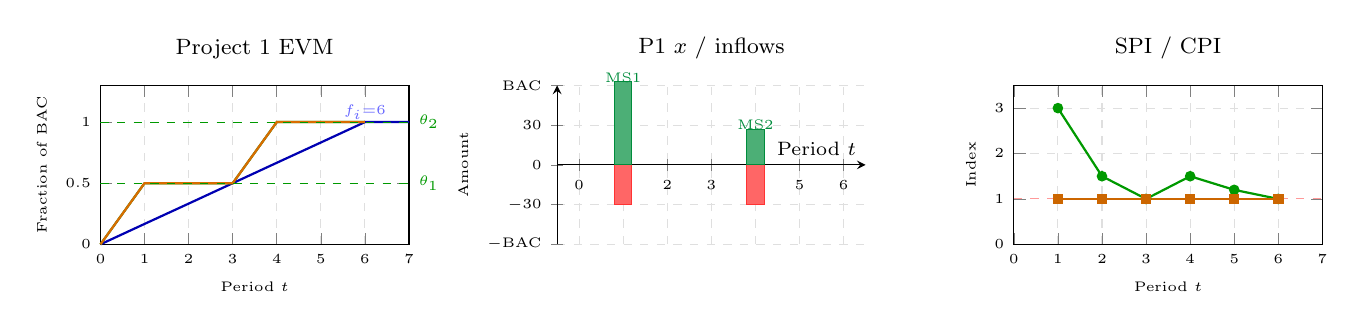
\begin{tikzpicture}[font=\footnotesize]
\begin{scope}
\begin{axis}[
    name=evmmpk_p1,
    width=5.5cm, height=3.6cm,
    title={\footnotesize Project 1 EVM},
    xlabel={Period $t$}, ylabel={Fraction of $\BAC$},
    xmin=0, xmax=7, ymin=0, ymax=1.30,
    xtick={0,1,2,3,4,5,6,7},
    ytick={0,0.5,1},
    grid=major, grid style={dashed,gray!25},
    tick label style={font=\tiny},
    label style={font=\tiny}, title style={font=\tiny},
    clip=false,
  ]
  \addplot[thick,blue!70!black] coordinates {(0,0) (1,0.167) (2,0.333) (3,0.5) (4,0.667) (5,0.833) (6,1) (7,1)};
  \addplot[thick,green!55!black] coordinates {(0,0) (1,0.5) (2,0.5) (3,0.5) (4,1) (5,1) (6,1)};
  \addplot[thick,orange!85!black] coordinates {(0,0) (1,0.5) (2,0.5) (3,0.5) (4,1) (5,1) (6,1)};
  \draw[green!60!black,dashed,thin] (axis cs:0,0.5)--(axis cs:7,0.5) node[right,green!60!black,font=\tiny] {$\theta_{1}$};
  \draw[green!60!black,dashed,thin] (axis cs:0,1)--(axis cs:7,1) node[right,green!60!black,font=\tiny] {$\theta_{2}$};
  \node[font=\tiny,blue!60] at (axis cs:6,1.08) {$f_i{=}6$};
\end{axis}
\end{scope}

\begin{scope}[xshift=5.8cm]
\begin{axis}[
    name=msmpk_p1,
    width=5.5cm, height=3.6cm,
    title={\footnotesize P1 $x$\ /\ inflows},
    xlabel={Period $t$}, ylabel={Amount},
    xmin=-0.5, xmax=6.5, ymin=-60, ymax=60,
    xtick={0,1,2,3,4,5,6},
    ytick={-60,-30,0,30,60},
    yticklabels={$-\BAC$,$-30$,$0$,$30$,$\BAC$},
    grid=major, grid style={dashed,gray!25},
    tick label style={font=\tiny},
    label style={font=\tiny}, title style={font=\tiny},
    axis x line=center, axis y line=left,
    clip=false,
  ]
  \addplot[ybar,bar width=0.22cm,fill=red!60,draw=red!80] coordinates {(1,-30) (4,-30)};
  \addplot[ybar,bar width=0.22cm,fill=msgreen!70,draw=msgreen] coordinates {(1,63) (4,27)};
  \node[font=\tiny,msgreen] at (axis cs:1,66) {MS1};
  \node[font=\tiny,msgreen] at (axis cs:4,30) {MS2};
\end{axis}
\end{scope}

\begin{scope}[xshift=11.6cm]
\begin{axis}[
    name=spicpimpk_p1,
    width=5.5cm, height=3.6cm,
    title={\footnotesize SPI / CPI},
    xlabel={Period $t$}, ylabel={Index},
    xmin=0, xmax=7, ymin=0, ymax=3.5,
    xtick={0,1,2,3,4,5,6,7},
    ytick={0,1,2,3},
    grid=major, grid style={dashed,gray!25},
    tick label style={font=\tiny},
    label style={font=\tiny}, title style={font=\tiny},
    clip=false,
  ]
  \draw[red!40,dashed,thin] (axis cs:0,1)--(axis cs:7,1);
  \addplot[thick,green!60!black,mark=*,mark size=1.5pt] coordinates {(1,3) (2,1.5) (3,1) (4,1.5) (5,1.2) (6,1)};
  \addplot[thick,orange!80!black,mark=square*,mark size=1.5pt] coordinates {(1,1) (2,1) (3,1) (4,1) (5,1) (6,1)};
\end{axis}
\end{scope}

\end{tikzpicture}
\vspace{0.3cm}

% === Project 2 row for MP-K ===
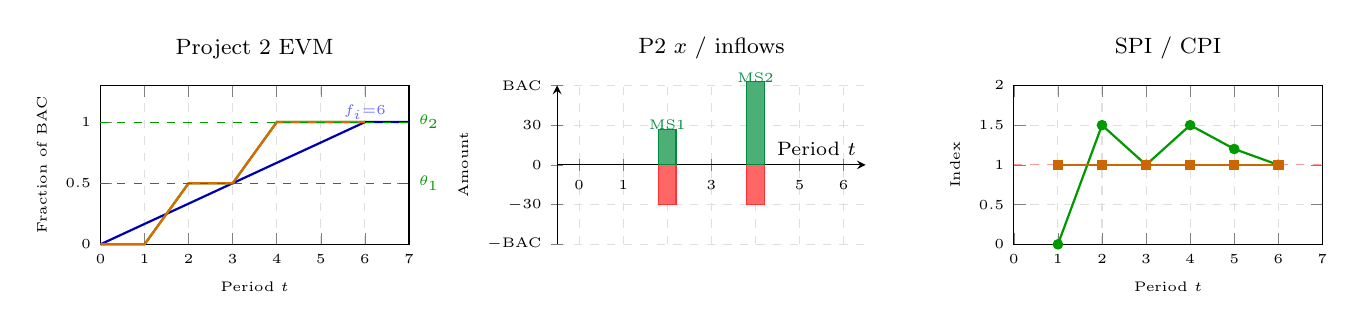
\begin{tikzpicture}[font=\footnotesize]
\begin{scope}
\begin{axis}[
    name=evmmpk_p2,
    width=5.5cm, height=3.6cm,
    title={\footnotesize Project 2 EVM},
    xlabel={Period $t$}, ylabel={Fraction of $\BAC$},
    xmin=0, xmax=7, ymin=0, ymax=1.30,
    xtick={0,1,2,3,4,5,6,7},
    ytick={0,0.5,1},
    grid=major, grid style={dashed,gray!25},
    tick label style={font=\tiny},
    label style={font=\tiny}, title style={font=\tiny},
    clip=false,
  ]
  \addplot[thick,blue!70!black] coordinates {(0,0) (1,0.167) (2,0.333) (3,0.5) (4,0.667) (5,0.833) (6,1) (7,1)};
  \addplot[thick,green!55!black] coordinates {(0,0) (1,0) (2,0.5) (3,0.5) (4,1) (5,1) (6,1)};
  \addplot[thick,orange!85!black] coordinates {(0,0) (1,0) (2,0.5) (3,0.5) (4,1) (5,1) (6,1)};
  \draw[green!60!black,dashed,thin] (axis cs:0,0.5)--(axis cs:7,0.5) node[right,green!60!black,font=\tiny] {$\theta_{1}$};
  \draw[green!60!black,dashed,thin] (axis cs:0,1)--(axis cs:7,1) node[right,green!60!black,font=\tiny] {$\theta_{2}$};
  \node[font=\tiny,blue!60] at (axis cs:6,1.08) {$f_i{=}6$};
\end{axis}
\end{scope}

\begin{scope}[xshift=5.8cm]
\begin{axis}[
    name=msmpk_p2,
    width=5.5cm, height=3.6cm,
    title={\footnotesize P2 $x$\ /\ inflows},
    xlabel={Period $t$}, ylabel={Amount},
    xmin=-0.5, xmax=6.5, ymin=-60, ymax=60,
    xtick={0,1,2,3,4,5,6},
    ytick={-60,-30,0,30,60},
    yticklabels={$-\BAC$,$-30$,$0$,$30$,$\BAC$},
    grid=major, grid style={dashed,gray!25},
    tick label style={font=\tiny},
    label style={font=\tiny}, title style={font=\tiny},
    axis x line=center, axis y line=left,
    clip=false,
  ]
  \addplot[ybar,bar width=0.22cm,fill=red!60,draw=red!80] coordinates {(2,-30) (4,-30)};
  \addplot[ybar,bar width=0.22cm,fill=msgreen!70,draw=msgreen] coordinates {(2,27) (4,63)};
  \node[font=\tiny,msgreen] at (axis cs:2,30) {MS1};
  \node[font=\tiny,msgreen] at (axis cs:4,66) {MS2};
\end{axis}
\end{scope}

\begin{scope}[xshift=11.6cm]
\begin{axis}[
    name=spicpimpk_p2,
    width=5.5cm, height=3.6cm,
    title={\footnotesize SPI / CPI},
    xlabel={Period $t$}, ylabel={Index},
    xmin=0, xmax=7, ymin=0, ymax=2,
    xtick={0,1,2,3,4,5,6,7},
    ytick={0,0.5,1,1.5,2},
    grid=major, grid style={dashed,gray!25},
    tick label style={font=\tiny},
    label style={font=\tiny}, title style={font=\tiny},
    clip=false,
  ]
  \draw[red!40,dashed,thin] (axis cs:0,1)--(axis cs:7,1);
  \addplot[thick,green!60!black,mark=*,mark size=1.5pt] coordinates {(1,0) (2,1.5) (3,1) (4,1.5) (5,1.2) (6,1)};
  \addplot[thick,orange!80!black,mark=square*,mark size=1.5pt] coordinates {(1,1) (2,1) (3,1) (4,1) (5,1) (6,1)};
\end{axis}
\end{scope}

\end{tikzpicture}

\caption{MP-K project view (2-project). Outcome: \texttt{both_completed}. $Z^*=55.87$.}
\label{fig:mpk_project}
\end{figure}

\begin{figure}[htbp]
\centering
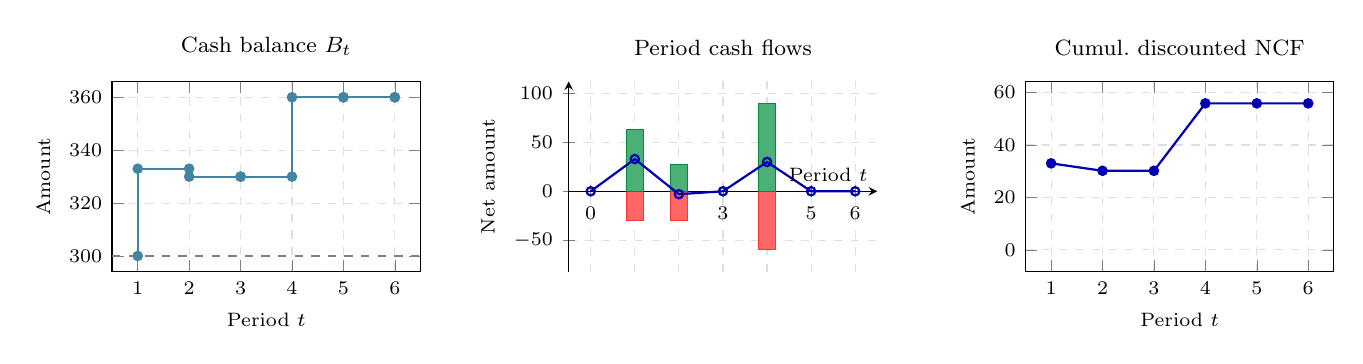
\begin{tikzpicture}[font=\footnotesize]
\begin{scope}
\begin{axis}[
    width=5.5cm, height=4.0cm,
    title={\footnotesize Cash balance $B_t$},
    xlabel={Period $t$}, ylabel={Amount},
    xmin=0.5, xmax=6.5,
    ymin=294, ymax=366,
    xtick={1,2,3,4,5,6},
    ytick={300,320,340,360},
    grid=major, grid style={dashed,gray!25},
    tick label style={font=\scriptsize},
    label style={font=\scriptsize}, title style={font=\scriptsize},
  ]
  \addplot[thick,cyan!60!black,mark=*,mark size=1.5pt] coordinates {(1,300) (1,333) (2,333) (2,330) (3,330) (3,330) (4,330) (4,360) (5,360) (5,360) (6,360) (6,360)};
  \draw[dashed,gray] (axis cs:0.5,300)--(axis cs:6.5,300) node[right,font=\tiny,gray] {$B_1$};
\end{axis}
\end{scope}

\begin{scope}[xshift=5.8cm]
\begin{axis}[
    width=5.5cm, height=4.0cm,
    title={\footnotesize Period cash flows},
    xlabel={Period $t$}, ylabel={Net amount},
    xmin=-0.5, xmax=6.5,
    ymin=-82.5, ymax=112.5,
    xtick={0,1,2,3,4,5,6},
    ytick={-50,0,50,100},
    grid=major, grid style={dashed,gray!25},
    tick label style={font=\scriptsize},
    label style={font=\scriptsize}, title style={font=\scriptsize},
    axis x line=center, axis y line=left,
    clip=false,
  ]
  \addplot[ybar,bar width=0.22cm,fill=red!60,draw=red!80] coordinates {(1,-30) (2,-30) (4,-60)};
  \addplot[ybar,bar width=0.22cm,fill=msgreen!70,draw=msgreen] coordinates {(1,63) (2,27) (4,90)};
  \addplot[thick,blue!70!black,mark=o,mark size=1.5pt] coordinates {(0,0) (1,33) (2,-3) (3,0) (4,30) (5,0) (6,0)};
\end{axis}
\end{scope}

\begin{scope}[xshift=11.6cm]
\begin{axis}[
    width=5.5cm, height=4.0cm,
    title={\footnotesize Cumul.\ discounted NCF},
    xlabel={Period $t$}, ylabel={Amount},
    xmin=0.5, xmax=6.5,
    ymin=-8.381, ymax=64.252,
    xtick={1,2,3,4,5,6},
    ytick={0,20,40,60},
    grid=major, grid style={dashed,gray!25},
    tick label style={font=\scriptsize},
    label style={font=\scriptsize}, title style={font=\scriptsize},
  ]
  \addplot[thick,blue!70!black,mark=*,mark size=1.5pt] coordinates {(1,33) (2,30.15) (3,30.15) (4,55.871) (5,55.871) (6,55.871)};
\end{axis}
\end{scope}

\end{tikzpicture}
\caption{MP-K portfolio view. $Z^*=55.87$.}
\label{fig:mpk_portfolio}
\end{figure}

\newpage

\subsection*{MP-Kp  (Group~G2)}
\begin{center}
\begin{tabular}{ll}
\toprule
$n$,\;$H$ & $2$,\;$6$ \\
$\BAC_i$ & $(30, 30)$ \\
$CP_i$   & $(45, 45)$ \\
$B_1,\;\gamma$ & $20,\;0.95$ \\
$Z^*$ & $27.936$ \\
Outcome & \texttt{both_completed} \\
\bottomrule
\end{tabular}
\end{center}

\paragraph{Project 1 timeline.}
\begin{center}
\begin{tabular}{rrrrrrrrrrl}
\toprule
$t$ & $x$ & $P$ & BCWS & BCWP & ACWP & SPI & CPI & $\tau$ & MS & $R_{\mathrm{net}}$\\
\midrule
1 & 15 & 0.5 & 0.167 & 0.5 & 0.5 & 3 & 1 & 2 & \texttt{1} & 31.5 \\
2 & 0 & 0.5 & 0.333 & 0.5 & 0.5 & 1.5 & 1 & 2 & \texttt{---} & 0 \\
3 & 0 & 0.5 & 0.5 & 0.5 & 0.5 & 1 & 1 & 2 & \texttt{---} & 0 \\
4 & 15 & 1 & 0.667 & 1 & 1 & 1.5 & 1 & 2 & \texttt{2} & 13.5 \\
5 & 0 & 1 & 0.833 & 1 & 1 & 1.2 & 1 & 2 & \texttt{---} & 0 \\
6 & 0 & 1 & 1 & 1 & 1 & 1 & 1 & 2 & \texttt{---} & 0 \\
\bottomrule
\end{tabular}
\end{center}
\paragraph{Project 2 timeline.}
\begin{center}
\begin{tabular}{rrrrrrrrrrl}
\toprule
$t$ & $x$ & $P$ & BCWS & BCWP & ACWP & SPI & CPI & $\tau$ & MS & $R_{\mathrm{net}}$\\
\midrule
1 & 0 & 0 & 0.167 & 0 & 0 & 0 & 1 & 2 & \texttt{---} & 0 \\
2 & 15 & 0.5 & 0.333 & 0.5 & 0.5 & 1.5 & 1 & 2 & \texttt{1} & 13.5 \\
3 & 0 & 0.5 & 0.5 & 0.5 & 0.5 & 1 & 1 & 2 & \texttt{---} & 0 \\
4 & 15 & 1 & 0.667 & 1 & 1 & 1.5 & 1 & 2 & \texttt{2} & 31.5 \\
5 & 0 & 1 & 0.833 & 1 & 1 & 1.2 & 1 & 2 & \texttt{---} & 0 \\
6 & 0 & 1 & 1 & 1 & 1 & 1 & 1 & 2 & \texttt{---} & 0 \\
\bottomrule
\end{tabular}
\end{center}
\paragraph{Portfolio strip.}
\begin{center}
\begin{tabular}{rrrrrrr}
\toprule
$t$ & $B_t$ & $\Sigma\mathrm{In}$ & $\Sigma\mathrm{Out}$ & $\Sigma\mathrm{Net}$ & $\gamma^{t-1}\mathrm{Net}$ & $Z_t^{\mathrm{cum}}$\\
\midrule
1 & 36.5 & 31.5 & 15 & 16.5 & 16.5 & 16.5 \\
2 & 35 & 13.5 & 15 & -1.5 & -1.425 & 15.075 \\
3 & 35 & 0 & 0 & 0 & 0 & 15.075 \\
4 & 50 & 45 & 30 & 15 & 12.861 & 27.936 \\
5 & 50 & 0 & 0 & 0 & 0 & 27.936 \\
6 & 50 & 0 & 0 & 0 & 0 & 27.936 \\
\bottomrule
\end{tabular}
\end{center}

\begin{figure}[htbp]
\centering
% === Project 1 row for MP-Kp ===
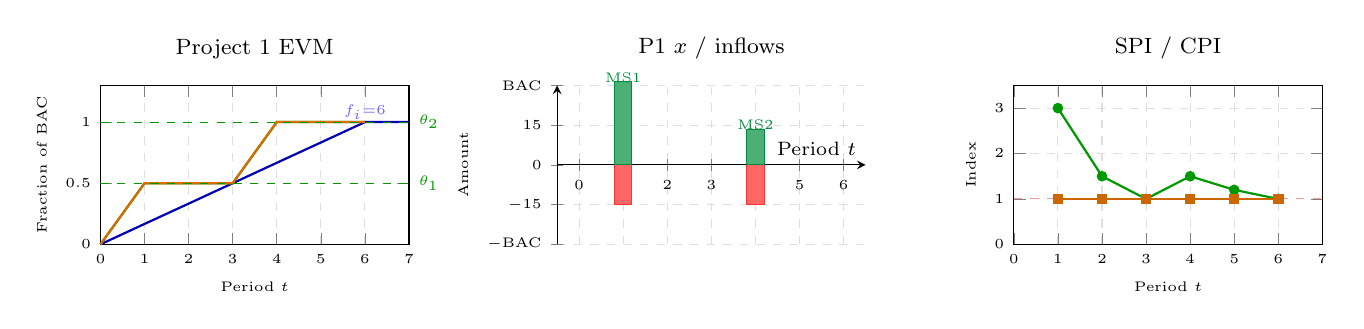
\begin{tikzpicture}[font=\footnotesize]
\begin{scope}
\begin{axis}[
    name=evmmpkp_p1,
    width=5.5cm, height=3.6cm,
    title={\footnotesize Project 1 EVM},
    xlabel={Period $t$}, ylabel={Fraction of $\BAC$},
    xmin=0, xmax=7, ymin=0, ymax=1.30,
    xtick={0,1,2,3,4,5,6,7},
    ytick={0,0.5,1},
    grid=major, grid style={dashed,gray!25},
    tick label style={font=\tiny},
    label style={font=\tiny}, title style={font=\tiny},
    clip=false,
  ]
  \addplot[thick,blue!70!black] coordinates {(0,0) (1,0.167) (2,0.333) (3,0.5) (4,0.667) (5,0.833) (6,1) (7,1)};
  \addplot[thick,green!55!black] coordinates {(0,0) (1,0.5) (2,0.5) (3,0.5) (4,1) (5,1) (6,1)};
  \addplot[thick,orange!85!black] coordinates {(0,0) (1,0.5) (2,0.5) (3,0.5) (4,1) (5,1) (6,1)};
  \draw[green!60!black,dashed,thin] (axis cs:0,0.5)--(axis cs:7,0.5) node[right,green!60!black,font=\tiny] {$\theta_{1}$};
  \draw[green!60!black,dashed,thin] (axis cs:0,1)--(axis cs:7,1) node[right,green!60!black,font=\tiny] {$\theta_{2}$};
  \node[font=\tiny,blue!60] at (axis cs:6,1.08) {$f_i{=}6$};
\end{axis}
\end{scope}

\begin{scope}[xshift=5.8cm]
\begin{axis}[
    name=msmpkp_p1,
    width=5.5cm, height=3.6cm,
    title={\footnotesize P1 $x$\ /\ inflows},
    xlabel={Period $t$}, ylabel={Amount},
    xmin=-0.5, xmax=6.5, ymin=-30, ymax=30,
    xtick={0,1,2,3,4,5,6},
    ytick={-30,-15,0,15,30},
    yticklabels={$-\BAC$,$-15$,$0$,$15$,$\BAC$},
    grid=major, grid style={dashed,gray!25},
    tick label style={font=\tiny},
    label style={font=\tiny}, title style={font=\tiny},
    axis x line=center, axis y line=left,
    clip=false,
  ]
  \addplot[ybar,bar width=0.22cm,fill=red!60,draw=red!80] coordinates {(1,-15) (4,-15)};
  \addplot[ybar,bar width=0.22cm,fill=msgreen!70,draw=msgreen] coordinates {(1,31.5) (4,13.5)};
  \node[font=\tiny,msgreen] at (axis cs:1,33) {MS1};
  \node[font=\tiny,msgreen] at (axis cs:4,15) {MS2};
\end{axis}
\end{scope}

\begin{scope}[xshift=11.6cm]
\begin{axis}[
    name=spicpimpkp_p1,
    width=5.5cm, height=3.6cm,
    title={\footnotesize SPI / CPI},
    xlabel={Period $t$}, ylabel={Index},
    xmin=0, xmax=7, ymin=0, ymax=3.5,
    xtick={0,1,2,3,4,5,6,7},
    ytick={0,1,2,3},
    grid=major, grid style={dashed,gray!25},
    tick label style={font=\tiny},
    label style={font=\tiny}, title style={font=\tiny},
    clip=false,
  ]
  \draw[red!40,dashed,thin] (axis cs:0,1)--(axis cs:7,1);
  \addplot[thick,green!60!black,mark=*,mark size=1.5pt] coordinates {(1,3) (2,1.5) (3,1) (4,1.5) (5,1.2) (6,1)};
  \addplot[thick,orange!80!black,mark=square*,mark size=1.5pt] coordinates {(1,1) (2,1) (3,1) (4,1) (5,1) (6,1)};
\end{axis}
\end{scope}

\end{tikzpicture}
\vspace{0.3cm}

% === Project 2 row for MP-Kp ===
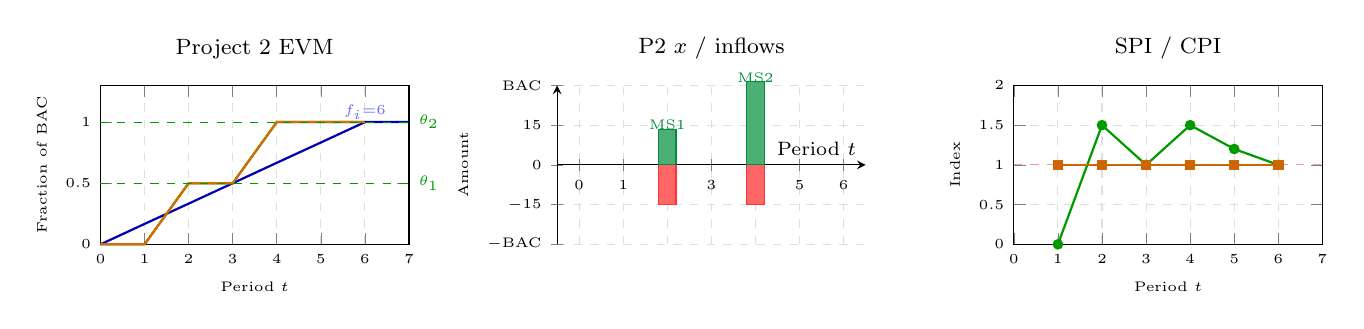
\begin{tikzpicture}[font=\footnotesize]
\begin{scope}
\begin{axis}[
    name=evmmpkp_p2,
    width=5.5cm, height=3.6cm,
    title={\footnotesize Project 2 EVM},
    xlabel={Period $t$}, ylabel={Fraction of $\BAC$},
    xmin=0, xmax=7, ymin=0, ymax=1.30,
    xtick={0,1,2,3,4,5,6,7},
    ytick={0,0.5,1},
    grid=major, grid style={dashed,gray!25},
    tick label style={font=\tiny},
    label style={font=\tiny}, title style={font=\tiny},
    clip=false,
  ]
  \addplot[thick,blue!70!black] coordinates {(0,0) (1,0.167) (2,0.333) (3,0.5) (4,0.667) (5,0.833) (6,1) (7,1)};
  \addplot[thick,green!55!black] coordinates {(0,0) (1,0) (2,0.5) (3,0.5) (4,1) (5,1) (6,1)};
  \addplot[thick,orange!85!black] coordinates {(0,0) (1,0) (2,0.5) (3,0.5) (4,1) (5,1) (6,1)};
  \draw[green!60!black,dashed,thin] (axis cs:0,0.5)--(axis cs:7,0.5) node[right,green!60!black,font=\tiny] {$\theta_{1}$};
  \draw[green!60!black,dashed,thin] (axis cs:0,1)--(axis cs:7,1) node[right,green!60!black,font=\tiny] {$\theta_{2}$};
  \node[font=\tiny,blue!60] at (axis cs:6,1.08) {$f_i{=}6$};
\end{axis}
\end{scope}

\begin{scope}[xshift=5.8cm]
\begin{axis}[
    name=msmpkp_p2,
    width=5.5cm, height=3.6cm,
    title={\footnotesize P2 $x$\ /\ inflows},
    xlabel={Period $t$}, ylabel={Amount},
    xmin=-0.5, xmax=6.5, ymin=-30, ymax=30,
    xtick={0,1,2,3,4,5,6},
    ytick={-30,-15,0,15,30},
    yticklabels={$-\BAC$,$-15$,$0$,$15$,$\BAC$},
    grid=major, grid style={dashed,gray!25},
    tick label style={font=\tiny},
    label style={font=\tiny}, title style={font=\tiny},
    axis x line=center, axis y line=left,
    clip=false,
  ]
  \addplot[ybar,bar width=0.22cm,fill=red!60,draw=red!80] coordinates {(2,-15) (4,-15)};
  \addplot[ybar,bar width=0.22cm,fill=msgreen!70,draw=msgreen] coordinates {(2,13.5) (4,31.5)};
  \node[font=\tiny,msgreen] at (axis cs:2,15) {MS1};
  \node[font=\tiny,msgreen] at (axis cs:4,33) {MS2};
\end{axis}
\end{scope}

\begin{scope}[xshift=11.6cm]
\begin{axis}[
    name=spicpimpkp_p2,
    width=5.5cm, height=3.6cm,
    title={\footnotesize SPI / CPI},
    xlabel={Period $t$}, ylabel={Index},
    xmin=0, xmax=7, ymin=0, ymax=2,
    xtick={0,1,2,3,4,5,6,7},
    ytick={0,0.5,1,1.5,2},
    grid=major, grid style={dashed,gray!25},
    tick label style={font=\tiny},
    label style={font=\tiny}, title style={font=\tiny},
    clip=false,
  ]
  \draw[red!40,dashed,thin] (axis cs:0,1)--(axis cs:7,1);
  \addplot[thick,green!60!black,mark=*,mark size=1.5pt] coordinates {(1,0) (2,1.5) (3,1) (4,1.5) (5,1.2) (6,1)};
  \addplot[thick,orange!80!black,mark=square*,mark size=1.5pt] coordinates {(1,1) (2,1) (3,1) (4,1) (5,1) (6,1)};
\end{axis}
\end{scope}

\end{tikzpicture}

\caption{MP-Kp project view (2-project). Outcome: \texttt{both_completed}. $Z^*=27.936$.}
\label{fig:mpkp_project}
\end{figure}

\begin{figure}[htbp]
\centering
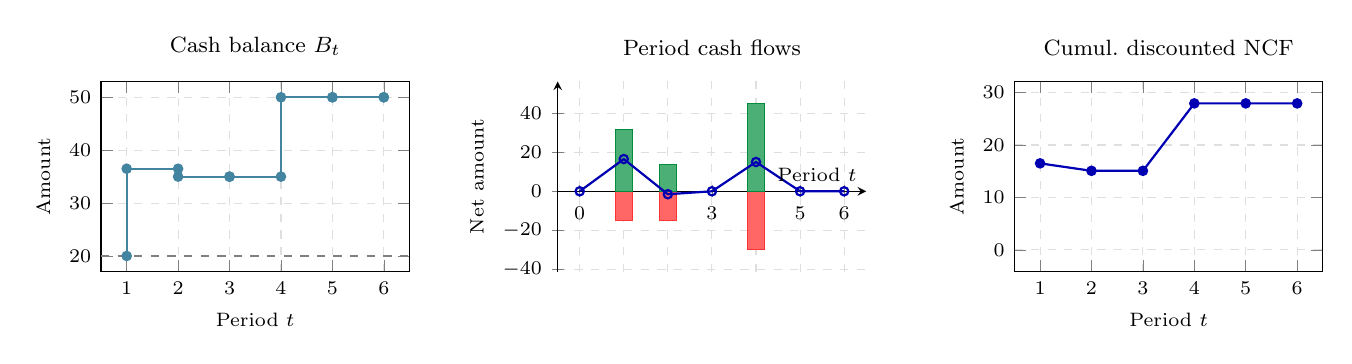
\begin{tikzpicture}[font=\footnotesize]
\begin{scope}
\begin{axis}[
    width=5.5cm, height=4.0cm,
    title={\footnotesize Cash balance $B_t$},
    xlabel={Period $t$}, ylabel={Amount},
    xmin=0.5, xmax=6.5,
    ymin=17, ymax=53,
    xtick={1,2,3,4,5,6},
    ytick={20,30,40,50},
    grid=major, grid style={dashed,gray!25},
    tick label style={font=\scriptsize},
    label style={font=\scriptsize}, title style={font=\scriptsize},
  ]
  \addplot[thick,cyan!60!black,mark=*,mark size=1.5pt] coordinates {(1,20) (1,36.5) (2,36.5) (2,35) (3,35) (3,35) (4,35) (4,50) (5,50) (5,50) (6,50) (6,50)};
  \draw[dashed,gray] (axis cs:0.5,20)--(axis cs:6.5,20) node[right,font=\tiny,gray] {$B_1$};
\end{axis}
\end{scope}

\begin{scope}[xshift=5.8cm]
\begin{axis}[
    width=5.5cm, height=4.0cm,
    title={\footnotesize Period cash flows},
    xlabel={Period $t$}, ylabel={Net amount},
    xmin=-0.5, xmax=6.5,
    ymin=-41.25, ymax=56.25,
    xtick={0,1,2,3,4,5,6},
    ytick={-40,-20,0,20,40},
    grid=major, grid style={dashed,gray!25},
    tick label style={font=\scriptsize},
    label style={font=\scriptsize}, title style={font=\scriptsize},
    axis x line=center, axis y line=left,
    clip=false,
  ]
  \addplot[ybar,bar width=0.22cm,fill=red!60,draw=red!80] coordinates {(1,-15) (2,-15) (4,-30)};
  \addplot[ybar,bar width=0.22cm,fill=msgreen!70,draw=msgreen] coordinates {(1,31.5) (2,13.5) (4,45)};
  \addplot[thick,blue!70!black,mark=o,mark size=1.5pt] coordinates {(0,0) (1,16.5) (2,-1.5) (3,0) (4,15) (5,0) (6,0)};
\end{axis}
\end{scope}

\begin{scope}[xshift=11.6cm]
\begin{axis}[
    width=5.5cm, height=4.0cm,
    title={\footnotesize Cumul.\ discounted NCF},
    xlabel={Period $t$}, ylabel={Amount},
    xmin=0.5, xmax=6.5,
    ymin=-4.19, ymax=32.126,
    xtick={1,2,3,4,5,6},
    ytick={0,10,20,30},
    grid=major, grid style={dashed,gray!25},
    tick label style={font=\scriptsize},
    label style={font=\scriptsize}, title style={font=\scriptsize},
  ]
  \addplot[thick,blue!70!black,mark=*,mark size=1.5pt] coordinates {(1,16.5) (2,15.075) (3,15.075) (4,27.936) (5,27.936) (6,27.936)};
\end{axis}
\end{scope}

\end{tikzpicture}
\caption{MP-Kp portfolio view. $Z^*=27.936$.}
\label{fig:mpkp_portfolio}
\end{figure}

\newpage

\subsection*{SP-L  (Group~G2)}
\begin{center}
\begin{tabular}{ll}
\toprule
$n$,\;$H$ & $1$,\;$6$ \\
$\BAC,\;CP$ & $100,\;170$ \\
$s_i,\;f_i,\;D^{\mathrm{plan}}$ & $1,\;6,\;8$ \\
$\bar\eta$ & $0.7$ \\
$M,\;\theta$ & $1,\;(1)$ \\
$\phi,\;e_{i,j}$ & $(1),\;(6)$ \\
$\mu,\;\Omega,\;\tau^{\mathrm{tol}}$ & $0.1,\;1,\;2$ \\
$B_1,\;\gamma$ & $300,\;0.95$ \\
$Z^*$ & $9.298$ \\
Outcome & \texttt{completed} \\
\bottomrule
\end{tabular}
\end{center}

\begin{center}
\begin{tabular}{rrrrrrrrrrl}
\toprule
$t$ & $x$ & $P$ & BCWS & BCWP & ACWP & SPI & CPI & $\tau$ & MS & $R_{\mathrm{net}}$\\
\midrule
1 & 17.857 & 0.125 & 0.125 & 0.125 & 0.179 & 1 & 0.7 & 2 & \texttt{---} & 0 \\
2 & 17.857 & 0.25 & 0.25 & 0.25 & 0.357 & 1 & 0.7 & 2 & \texttt{---} & 0 \\
3 & 17.857 & 0.375 & 0.375 & 0.375 & 0.536 & 1 & 0.7 & 2 & \texttt{---} & 0 \\
4 & 17.857 & 0.5 & 0.5 & 0.5 & 0.714 & 1 & 0.7 & 2 & \texttt{---} & 0 \\
5 & 17.857 & 0.625 & 0.625 & 0.625 & 0.893 & 1 & 0.7 & 2 & \texttt{---} & 0 \\
6 & 53.571 & 1 & 0.75 & 1 & 1.429 & 1.333 & 0.7 & 2 & \texttt{1} & 170 \\
\bottomrule
\end{tabular}
\end{center}
\paragraph{Portfolio strip.}
\begin{center}
\begin{tabular}{rrrrrrr}
\toprule
$t$ & $B_t$ & $\Sigma\mathrm{In}$ & $\Sigma\mathrm{Out}$ & $\Sigma\mathrm{Net}$ & $\gamma^{t-1}\mathrm{Net}$ & $Z_t^{\mathrm{cum}}$\\
\midrule
1 & 282.1 & 0 & 17.857 & -17.857 & -17.857 & -17.857 \\
2 & 264.3 & 0 & 17.857 & -17.857 & -16.964 & -34.821 \\
3 & 246.4 & 0 & 17.857 & -17.857 & -16.116 & -50.938 \\
4 & 228.6 & 0 & 17.857 & -17.857 & -15.31 & -66.248 \\
5 & 210.7 & 0 & 17.857 & -17.857 & -14.545 & -80.793 \\
6 & 327.1 & 170 & 53.571 & 116.429 & 90.09 & 9.298 \\
\bottomrule
\end{tabular}
\end{center}

\begin{figure}[htbp]
\centering
% === Project 1 row for SP-L ===
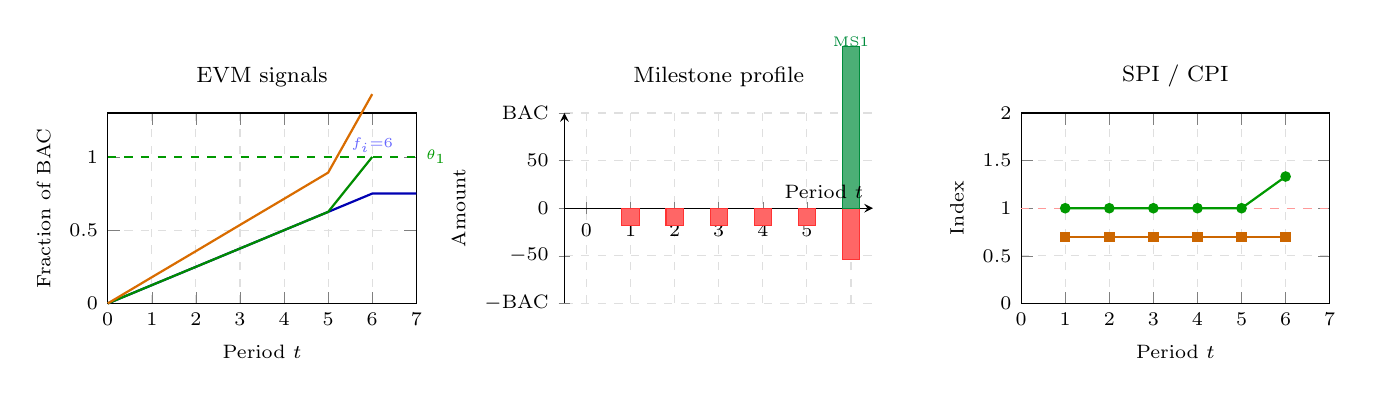
\begin{tikzpicture}[font=\footnotesize]
\begin{scope}
\begin{axis}[
    name=evmspl_p1,
    width=5.5cm, height=4.0cm,
    title={\footnotesize EVM signals},
    xlabel={Period $t$}, ylabel={Fraction of $\BAC$},
    xmin=0, xmax=7, ymin=0, ymax=1.30,
    xtick={0,1,2,3,4,5,6,7},
    ytick={0,0.5,1},
    grid=major, grid style={dashed,gray!25},
    tick label style={font=\scriptsize},
    label style={font=\scriptsize}, title style={font=\scriptsize},
    clip=false,
  ]
  \addplot[thick,blue!70!black] coordinates {(0,0) (1,0.125) (2,0.25) (3,0.375) (4,0.5) (5,0.625) (6,0.75) (7,0.75)};
  \addplot[thick,green!55!black] coordinates {(0,0) (1,0.125) (2,0.25) (3,0.375) (4,0.5) (5,0.625) (6,1)};
  \addplot[thick,orange!85!black] coordinates {(0,0) (1,0.179) (2,0.357) (3,0.536) (4,0.714) (5,0.893) (6,1.429)};
  \draw[green!60!black,dashed,thin] (axis cs:0,1)--(axis cs:7,1) node[right,green!60!black,font=\tiny] {$\theta_{1}$};
  \node[font=\tiny,blue!60] at (axis cs:6,1.08) {$f_i{=}6$};
\end{axis}
\end{scope}

\begin{scope}[xshift=5.8cm]
\begin{axis}[
    name=msspl_p1,
    width=5.5cm, height=4.0cm,
    title={\footnotesize Milestone profile},
    xlabel={Period $t$}, ylabel={Amount},
    xmin=-0.5, xmax=6.5, ymin=-100, ymax=100,
    xtick={0,1,2,3,4,5,6},
    ytick={-100,-50,0,50,100},
    yticklabels={$-\BAC$,$-50$,$0$,$50$,$\BAC$},
    grid=major, grid style={dashed,gray!25},
    tick label style={font=\scriptsize},
    label style={font=\scriptsize}, title style={font=\scriptsize},
    axis x line=center, axis y line=left,
    clip=false,
  ]
  \addplot[ybar,bar width=0.22cm,fill=red!60,draw=red!80] coordinates {(1,-17.857) (2,-17.857) (3,-17.857) (4,-17.857) (5,-17.857) (6,-53.571)};
  \addplot[ybar,bar width=0.22cm,fill=msgreen!70,draw=msgreen] coordinates {(6,170)};
  \node[font=\tiny,msgreen] at (axis cs:6,175) {MS1};
\end{axis}
\end{scope}

\begin{scope}[xshift=11.6cm]
\begin{axis}[
    name=spicpispl_p1,
    width=5.5cm, height=4.0cm,
    title={\footnotesize SPI / CPI},
    xlabel={Period $t$}, ylabel={Index},
    xmin=0, xmax=7, ymin=0, ymax=2,
    xtick={0,1,2,3,4,5,6,7},
    ytick={0,0.5,1,1.5,2},
    grid=major, grid style={dashed,gray!25},
    tick label style={font=\scriptsize},
    label style={font=\scriptsize}, title style={font=\scriptsize},
    clip=false,
  ]
  \draw[red!40,dashed,thin] (axis cs:0,1)--(axis cs:7,1);
  \addplot[thick,green!60!black,mark=*,mark size=1.5pt] coordinates {(1,1) (2,1) (3,1) (4,1) (5,1) (6,1.333)};
  \addplot[thick,orange!80!black,mark=square*,mark size=1.5pt] coordinates {(1,0.7) (2,0.7) (3,0.7) (4,0.7) (5,0.7) (6,0.7)};
\end{axis}
\end{scope}

\end{tikzpicture}

\caption{SP-L project view (single-project). Outcome: \texttt{completed}. $Z^*=9.298$.}
\label{fig:spl_project}
\end{figure}

\begin{figure}[htbp]
\centering
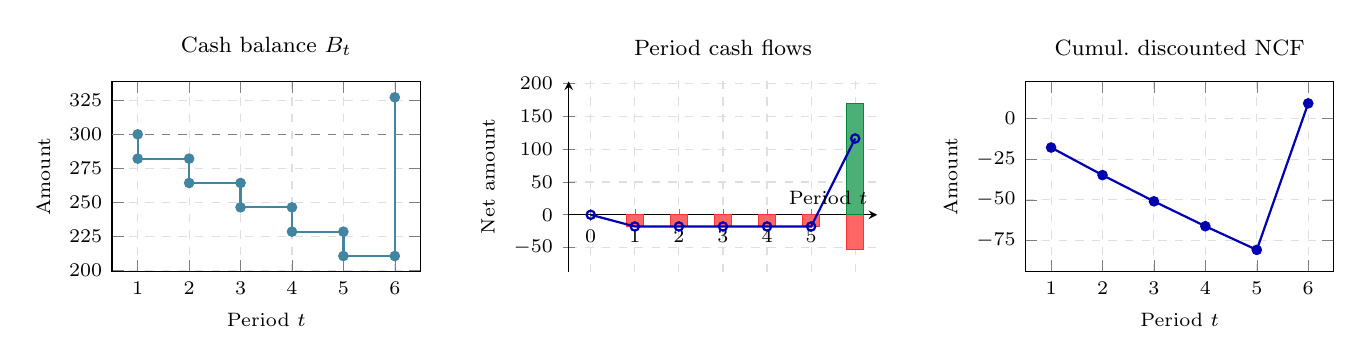
\begin{tikzpicture}[font=\footnotesize]
\begin{scope}
\begin{axis}[
    width=5.5cm, height=4.0cm,
    title={\footnotesize Cash balance $B_t$},
    xlabel={Period $t$}, ylabel={Amount},
    xmin=0.5, xmax=6.5,
    ymin=199.1, ymax=338.8,
    xtick={1,2,3,4,5,6},
    ytick={200,225,250,275,300,325},
    grid=major, grid style={dashed,gray!25},
    tick label style={font=\scriptsize},
    label style={font=\scriptsize}, title style={font=\scriptsize},
  ]
  \addplot[thick,cyan!60!black,mark=*,mark size=1.5pt] coordinates {(1,300) (1,282.143) (2,282.143) (2,264.286) (3,264.286) (3,246.429) (4,246.429) (4,228.571) (5,228.571) (5,210.714) (6,210.714) (6,327.143)};
  \draw[dashed,gray] (axis cs:0.5,300)--(axis cs:6.5,300) node[right,font=\tiny,gray] {$B_1$};
\end{axis}
\end{scope}

\begin{scope}[xshift=5.8cm]
\begin{axis}[
    width=5.5cm, height=4.0cm,
    title={\footnotesize Period cash flows},
    xlabel={Period $t$}, ylabel={Net amount},
    xmin=-0.5, xmax=6.5,
    ymin=-87.107, ymax=203.536,
    xtick={0,1,2,3,4,5,6},
    ytick={-50,0,50,100,150,200},
    grid=major, grid style={dashed,gray!25},
    tick label style={font=\scriptsize},
    label style={font=\scriptsize}, title style={font=\scriptsize},
    axis x line=center, axis y line=left,
    clip=false,
  ]
  \addplot[ybar,bar width=0.22cm,fill=red!60,draw=red!80] coordinates {(1,-17.857) (2,-17.857) (3,-17.857) (4,-17.857) (5,-17.857) (6,-53.571)};
  \addplot[ybar,bar width=0.22cm,fill=msgreen!70,draw=msgreen] coordinates {(6,170)};
  \addplot[thick,blue!70!black,mark=o,mark size=1.5pt] coordinates {(0,0) (1,-17.857) (2,-17.857) (3,-17.857) (4,-17.857) (5,-17.857) (6,116.429)};
\end{axis}
\end{scope}

\begin{scope}[xshift=11.6cm]
\begin{axis}[
    width=5.5cm, height=4.0cm,
    title={\footnotesize Cumul.\ discounted NCF},
    xlabel={Period $t$}, ylabel={Amount},
    xmin=0.5, xmax=6.5,
    ymin=-94.306, ymax=22.811,
    xtick={1,2,3,4,5,6},
    ytick={-75,-50,-25,0},
    grid=major, grid style={dashed,gray!25},
    tick label style={font=\scriptsize},
    label style={font=\scriptsize}, title style={font=\scriptsize},
  ]
  \addplot[thick,blue!70!black,mark=*,mark size=1.5pt] coordinates {(1,-17.857) (2,-34.821) (3,-50.938) (4,-66.248) (5,-80.793) (6,9.298)};
\end{axis}
\end{scope}

\end{tikzpicture}
\caption{SP-L portfolio view. $Z^*=9.298$.}
\label{fig:spl_portfolio}
\end{figure}

\newpage

\subsection*{SP-Lp  (Group~G2)}
\begin{center}
\begin{tabular}{ll}
\toprule
$n$,\;$H$ & $1$,\;$6$ \\
$\BAC,\;CP$ & $100,\;80$ \\
$s_i,\;f_i,\;D^{\mathrm{plan}}$ & $1,\;6,\;8$ \\
$\bar\eta$ & $0.7$ \\
$M,\;\theta$ & $1,\;(1)$ \\
$\phi,\;e_{i,j}$ & $(1),\;(6)$ \\
$\mu,\;\Omega,\;\tau^{\mathrm{tol}}$ & $0.1,\;1,\;2$ \\
$B_1,\;\gamma$ & $300,\;0.95$ \\
$Z^*$ & $0$ \\
Outcome & \texttt{terminated} \\
\bottomrule
\end{tabular}
\end{center}

\begin{center}
\begin{tabular}{rrrrrrrrrrl}
\toprule
$t$ & $x$ & $P$ & BCWS & BCWP & ACWP & SPI & CPI & $\tau$ & MS & $R_{\mathrm{net}}$\\
\midrule
1 & 0 & 0 & 0.125 & 0 & 0 & 0 & 1 & 2 & \texttt{---} & 0 \\
2 & 0 & 0 & 0.25 & 0 & 0 & 0 & 1 & 2 & \texttt{---} & 0 \\
3 & 0 & 0 & 0.375 & 0 & 0 & 0 & 1 & 2 & \texttt{---} & 0 \\
\bottomrule
\end{tabular}
\end{center}
\paragraph{Portfolio strip.}
\begin{center}
\begin{tabular}{rrrrrrr}
\toprule
$t$ & $B_t$ & $\Sigma\mathrm{In}$ & $\Sigma\mathrm{Out}$ & $\Sigma\mathrm{Net}$ & $\gamma^{t-1}\mathrm{Net}$ & $Z_t^{\mathrm{cum}}$\\
\midrule
1 & 300 & 0 & 0 & 0 & 0 & 0 \\
2 & 300 & 0 & 0 & 0 & 0 & 0 \\
3 & 300 & 0 & 0 & 0 & 0 & 0 \\
4 & 300 & 0 & 0 & 0 & 0 & 0 \\
5 & 300 & 0 & 0 & 0 & 0 & 0 \\
6 & 300 & 0 & 0 & 0 & 0 & 0 \\
\bottomrule
\end{tabular}
\end{center}

\begin{figure}[htbp]
\centering
% === Project 1 row for SP-Lp ===
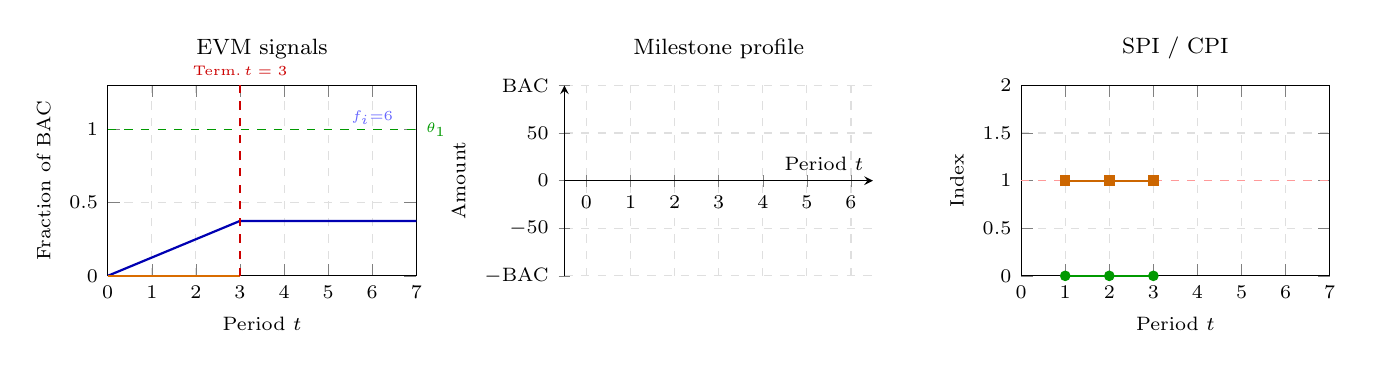
\begin{tikzpicture}[font=\footnotesize]
\begin{scope}
\begin{axis}[
    name=evmsplp_p1,
    width=5.5cm, height=4.0cm,
    title={\footnotesize EVM signals},
    xlabel={Period $t$}, ylabel={Fraction of $\BAC$},
    xmin=0, xmax=7, ymin=0, ymax=1.30,
    xtick={0,1,2,3,4,5,6,7},
    ytick={0,0.5,1},
    grid=major, grid style={dashed,gray!25},
    tick label style={font=\scriptsize},
    label style={font=\scriptsize}, title style={font=\scriptsize},
    clip=false,
  ]
  \addplot[thick,blue!70!black] coordinates {(0,0) (1,0.125) (2,0.25) (3,0.375) (7,0.375)};
  \addplot[thick,green!55!black] coordinates {(0,0) (1,0) (2,0) (3,0)};
  \addplot[thick,orange!85!black] coordinates {(0,0) (1,0) (2,0) (3,0)};
  \draw[green!60!black,dashed,thin] (axis cs:0,1)--(axis cs:7,1) node[right,green!60!black,font=\tiny] {$\theta_{1}$};
  \node[font=\tiny,blue!60] at (axis cs:6,1.08) {$f_i{=}6$};
  \draw[red!80!black,dashed,thick] (axis cs:3,0)--(axis cs:3,1.30) node[above,font=\tiny,red!80!black] {Term.\,$t=3$};
\end{axis}
\end{scope}

\begin{scope}[xshift=5.8cm]
\begin{axis}[
    name=mssplp_p1,
    width=5.5cm, height=4.0cm,
    title={\footnotesize Milestone profile},
    xlabel={Period $t$}, ylabel={Amount},
    xmin=-0.5, xmax=6.5, ymin=-100, ymax=100,
    xtick={0,1,2,3,4,5,6},
    ytick={-100,-50,0,50,100},
    yticklabels={$-\BAC$,$-50$,$0$,$50$,$\BAC$},
    grid=major, grid style={dashed,gray!25},
    tick label style={font=\scriptsize},
    label style={font=\scriptsize}, title style={font=\scriptsize},
    axis x line=center, axis y line=left,
    clip=false,
  ]
\end{axis}
\end{scope}

\begin{scope}[xshift=11.6cm]
\begin{axis}[
    name=spicpisplp_p1,
    width=5.5cm, height=4.0cm,
    title={\footnotesize SPI / CPI},
    xlabel={Period $t$}, ylabel={Index},
    xmin=0, xmax=7, ymin=0, ymax=2,
    xtick={0,1,2,3,4,5,6,7},
    ytick={0,0.5,1,1.5,2},
    grid=major, grid style={dashed,gray!25},
    tick label style={font=\scriptsize},
    label style={font=\scriptsize}, title style={font=\scriptsize},
    clip=false,
  ]
  \draw[red!40,dashed,thin] (axis cs:0,1)--(axis cs:7,1);
  \addplot[thick,green!60!black,mark=*,mark size=1.5pt] coordinates {(1,0) (2,0) (3,0)};
  \addplot[thick,orange!80!black,mark=square*,mark size=1.5pt] coordinates {(1,1) (2,1) (3,1)};
\end{axis}
\end{scope}

\end{tikzpicture}

\caption{SP-Lp project view (single-project). Outcome: \texttt{terminated}. $Z^*=0$.}
\label{fig:splp_project}
\end{figure}

\begin{figure}[htbp]
\centering
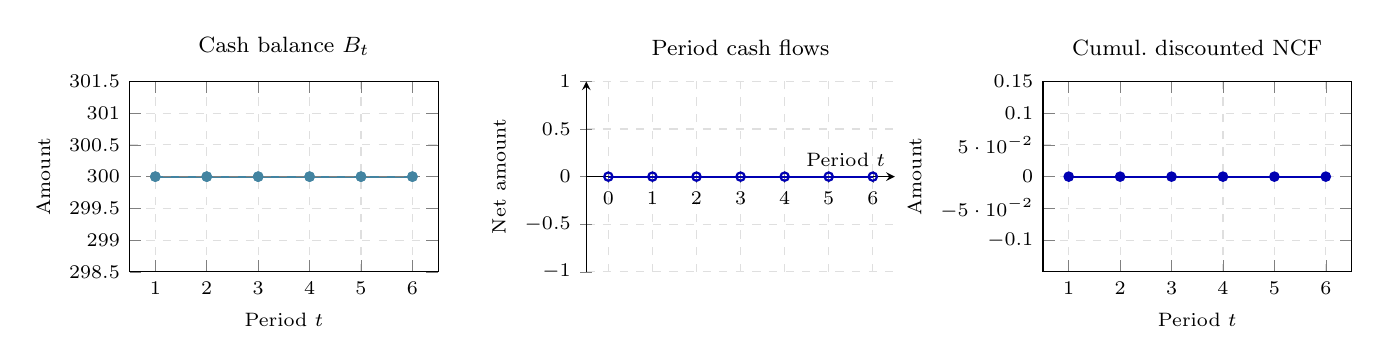
\begin{tikzpicture}[font=\footnotesize]
\begin{scope}
\begin{axis}[
    width=5.5cm, height=4.0cm,
    title={\footnotesize Cash balance $B_t$},
    xlabel={Period $t$}, ylabel={Amount},
    xmin=0.5, xmax=6.5,
    ymin=298.5, ymax=301.5,
    xtick={1,2,3,4,5,6},
    ytick={298.5,299,299.5,300,300.5,301,301.5},
    grid=major, grid style={dashed,gray!25},
    tick label style={font=\scriptsize},
    label style={font=\scriptsize}, title style={font=\scriptsize},
  ]
  \addplot[thick,cyan!60!black,mark=*,mark size=1.5pt] coordinates {(1,300) (1,300) (2,300) (2,300) (3,300) (3,300) (4,300) (4,300) (5,300) (5,300) (6,300) (6,300)};
  \draw[dashed,gray] (axis cs:0.5,300)--(axis cs:6.5,300) node[right,font=\tiny,gray] {$B_1$};
\end{axis}
\end{scope}

\begin{scope}[xshift=5.8cm]
\begin{axis}[
    width=5.5cm, height=4.0cm,
    title={\footnotesize Period cash flows},
    xlabel={Period $t$}, ylabel={Net amount},
    xmin=-0.5, xmax=6.5,
    ymin=-1, ymax=1,
    xtick={0,1,2,3,4,5,6},
    ytick={-1,-0.5,0,0.5,1},
    grid=major, grid style={dashed,gray!25},
    tick label style={font=\scriptsize},
    label style={font=\scriptsize}, title style={font=\scriptsize},
    axis x line=center, axis y line=left,
    clip=false,
  ]
  \addplot[thick,blue!70!black,mark=o,mark size=1.5pt] coordinates {(0,0) (1,0) (2,0) (3,0) (4,0) (5,0) (6,0)};
\end{axis}
\end{scope}

\begin{scope}[xshift=11.6cm]
\begin{axis}[
    width=5.5cm, height=4.0cm,
    title={\footnotesize Cumul.\ discounted NCF},
    xlabel={Period $t$}, ylabel={Amount},
    xmin=0.5, xmax=6.5,
    ymin=-0.15, ymax=0.15,
    xtick={1,2,3,4,5,6},
    ytick={-0.1,-0.05,0,0.05,0.1,0.15},
    grid=major, grid style={dashed,gray!25},
    tick label style={font=\scriptsize},
    label style={font=\scriptsize}, title style={font=\scriptsize},
  ]
  \addplot[thick,blue!70!black,mark=*,mark size=1.5pt] coordinates {(1,0) (2,0) (3,0) (4,0) (5,0) (6,0)};
\end{axis}
\end{scope}

\end{tikzpicture}
\caption{SP-Lp portfolio view. $Z^*=0$.}
\label{fig:splp_portfolio}
\end{figure}

\newpage

\subsection*{SP-M  (Group~G2)}
\begin{center}
\begin{tabular}{ll}
\toprule
$n$,\;$H$ & $2$,\;$6$ \\
$\BAC_i$ & $(60, 100)$ \\
$CP_i$   & $(90, 170)$ \\
$B_1,\;\gamma$ & $90,\;0.95$ \\
$Z^*$ & $39.298$ \\
Outcome & \texttt{both_completed} \\
\bottomrule
\end{tabular}
\end{center}

\paragraph{Project 1 timeline.}
\begin{center}
\begin{tabular}{rrrrrrrrrrl}
\toprule
$t$ & $x$ & $P$ & BCWS & BCWP & ACWP & SPI & CPI & $\tau$ & MS & $R_{\mathrm{net}}$\\
\midrule
1 & 60 & 1 & 0.5 & 1 & 1 & 2 & 1 & 2 & \texttt{1} & 90 \\
2 & 0 & 1 & 1 & 1 & 1 & 1 & 1 & 2 & \texttt{---} & 0 \\
\bottomrule
\end{tabular}
\end{center}
\paragraph{Project 2 timeline.}
\begin{center}
\begin{tabular}{rrrrrrrrrrl}
\toprule
$t$ & $x$ & $P$ & BCWS & BCWP & ACWP & SPI & CPI & $\tau$ & MS & $R_{\mathrm{net}}$\\
\midrule
1 & 17.857 & 0.125 & 0.125 & 0.125 & 0.179 & 1 & 0.7 & 1 & \texttt{---} & 0 \\
2 & 17.857 & 0.25 & 0.25 & 0.25 & 0.357 & 1 & 0.7 & 0 & \texttt{---} & 0 \\
3 & 17.857 & 0.375 & 0.375 & 0.375 & 0.536 & 1 & 0.7 & 0 & \texttt{---} & 0 \\
4 & 17.857 & 0.5 & 0.5 & 0.5 & 0.714 & 1 & 0.7 & 0 & \texttt{---} & 0 \\
5 & 17.857 & 0.625 & 0.625 & 0.625 & 0.893 & 1 & 0.7 & 0 & \texttt{---} & 0 \\
6 & 53.572 & 1 & 0.75 & 1 & 1.429 & 1.333 & 0.7 & 2 & \texttt{1} & 170 \\
\bottomrule
\end{tabular}
\end{center}
\paragraph{Portfolio strip.}
\begin{center}
\begin{tabular}{rrrrrrr}
\toprule
$t$ & $B_t$ & $\Sigma\mathrm{In}$ & $\Sigma\mathrm{Out}$ & $\Sigma\mathrm{Net}$ & $\gamma^{t-1}\mathrm{Net}$ & $Z_t^{\mathrm{cum}}$\\
\midrule
1 & 102.1 & 90 & 77.857 & 12.143 & 12.143 & 12.143 \\
2 & 84.3 & 0 & 17.857 & -17.857 & -16.964 & -4.821 \\
3 & 66.4 & 0 & 17.857 & -17.857 & -16.116 & -20.937 \\
4 & 48.6 & 0 & 17.857 & -17.857 & -15.31 & -36.248 \\
5 & 30.7 & 0 & 17.857 & -17.857 & -14.545 & -50.792 \\
6 & 147.1 & 170 & 53.572 & 116.428 & 90.09 & 39.298 \\
\bottomrule
\end{tabular}
\end{center}

\begin{figure}[htbp]
\centering
% === Project 1 row for SP-M ===
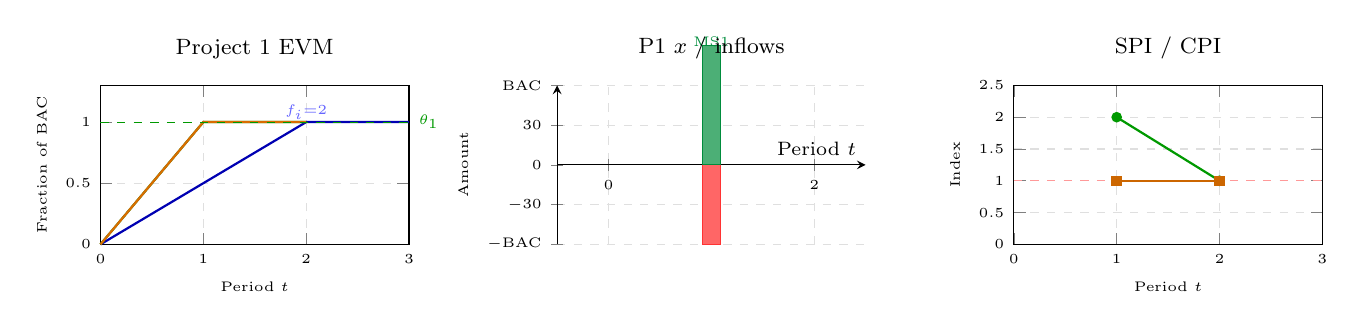
\begin{tikzpicture}[font=\footnotesize]
\begin{scope}
\begin{axis}[
    name=evmspm_p1,
    width=5.5cm, height=3.6cm,
    title={\footnotesize Project 1 EVM},
    xlabel={Period $t$}, ylabel={Fraction of $\BAC$},
    xmin=0, xmax=3, ymin=0, ymax=1.30,
    xtick={0,1,2,3},
    ytick={0,0.5,1},
    grid=major, grid style={dashed,gray!25},
    tick label style={font=\tiny},
    label style={font=\tiny}, title style={font=\tiny},
    clip=false,
  ]
  \addplot[thick,blue!70!black] coordinates {(0,0) (1,0.5) (2,1) (3,1)};
  \addplot[thick,green!55!black] coordinates {(0,0) (1,1) (2,1)};
  \addplot[thick,orange!85!black] coordinates {(0,0) (1,1) (2,1)};
  \draw[green!60!black,dashed,thin] (axis cs:0,1)--(axis cs:3,1) node[right,green!60!black,font=\tiny] {$\theta_{1}$};
  \node[font=\tiny,blue!60] at (axis cs:2,1.08) {$f_i{=}2$};
\end{axis}
\end{scope}

\begin{scope}[xshift=5.8cm]
\begin{axis}[
    name=msspm_p1,
    width=5.5cm, height=3.6cm,
    title={\footnotesize P1 $x$\ /\ inflows},
    xlabel={Period $t$}, ylabel={Amount},
    xmin=-0.5, xmax=2.5, ymin=-60, ymax=60,
    xtick={0,1,2},
    ytick={-60,-30,0,30,60},
    yticklabels={$-\BAC$,$-30$,$0$,$30$,$\BAC$},
    grid=major, grid style={dashed,gray!25},
    tick label style={font=\tiny},
    label style={font=\tiny}, title style={font=\tiny},
    axis x line=center, axis y line=left,
    clip=false,
  ]
  \addplot[ybar,bar width=0.22cm,fill=red!60,draw=red!80] coordinates {(1,-60)};
  \addplot[ybar,bar width=0.22cm,fill=msgreen!70,draw=msgreen] coordinates {(1,90)};
  \node[font=\tiny,msgreen] at (axis cs:1,93) {MS1};
\end{axis}
\end{scope}

\begin{scope}[xshift=11.6cm]
\begin{axis}[
    name=spicpispm_p1,
    width=5.5cm, height=3.6cm,
    title={\footnotesize SPI / CPI},
    xlabel={Period $t$}, ylabel={Index},
    xmin=0, xmax=3, ymin=0, ymax=2.5,
    xtick={0,1,2,3},
    ytick={0,0.5,1,1.5,2,2.5},
    grid=major, grid style={dashed,gray!25},
    tick label style={font=\tiny},
    label style={font=\tiny}, title style={font=\tiny},
    clip=false,
  ]
  \draw[red!40,dashed,thin] (axis cs:0,1)--(axis cs:3,1);
  \addplot[thick,green!60!black,mark=*,mark size=1.5pt] coordinates {(1,2) (2,1)};
  \addplot[thick,orange!80!black,mark=square*,mark size=1.5pt] coordinates {(1,1) (2,1)};
\end{axis}
\end{scope}

\end{tikzpicture}
\vspace{0.3cm}

% === Project 2 row for SP-M ===
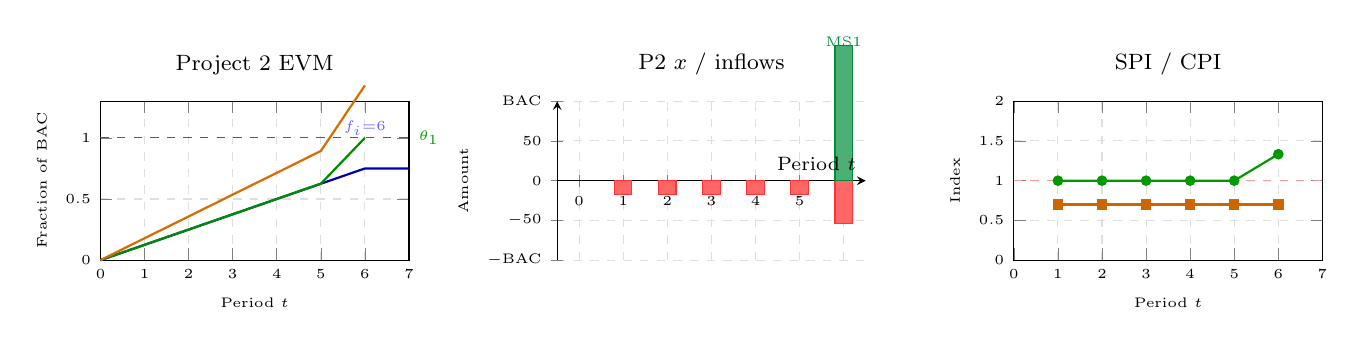
\begin{tikzpicture}[font=\footnotesize]
\begin{scope}
\begin{axis}[
    name=evmspm_p2,
    width=5.5cm, height=3.6cm,
    title={\footnotesize Project 2 EVM},
    xlabel={Period $t$}, ylabel={Fraction of $\BAC$},
    xmin=0, xmax=7, ymin=0, ymax=1.30,
    xtick={0,1,2,3,4,5,6,7},
    ytick={0,0.5,1},
    grid=major, grid style={dashed,gray!25},
    tick label style={font=\tiny},
    label style={font=\tiny}, title style={font=\tiny},
    clip=false,
  ]
  \addplot[thick,blue!70!black] coordinates {(0,0) (1,0.125) (2,0.25) (3,0.375) (4,0.5) (5,0.625) (6,0.75) (7,0.75)};
  \addplot[thick,green!55!black] coordinates {(0,0) (1,0.125) (2,0.25) (3,0.375) (4,0.5) (5,0.625) (6,1)};
  \addplot[thick,orange!85!black] coordinates {(0,0) (1,0.179) (2,0.357) (3,0.536) (4,0.714) (5,0.893) (6,1.429)};
  \draw[green!60!black,dashed,thin] (axis cs:0,1)--(axis cs:7,1) node[right,green!60!black,font=\tiny] {$\theta_{1}$};
  \node[font=\tiny,blue!60] at (axis cs:6,1.08) {$f_i{=}6$};
\end{axis}
\end{scope}

\begin{scope}[xshift=5.8cm]
\begin{axis}[
    name=msspm_p2,
    width=5.5cm, height=3.6cm,
    title={\footnotesize P2 $x$\ /\ inflows},
    xlabel={Period $t$}, ylabel={Amount},
    xmin=-0.5, xmax=6.5, ymin=-100, ymax=100,
    xtick={0,1,2,3,4,5,6},
    ytick={-100,-50,0,50,100},
    yticklabels={$-\BAC$,$-50$,$0$,$50$,$\BAC$},
    grid=major, grid style={dashed,gray!25},
    tick label style={font=\tiny},
    label style={font=\tiny}, title style={font=\tiny},
    axis x line=center, axis y line=left,
    clip=false,
  ]
  \addplot[ybar,bar width=0.22cm,fill=red!60,draw=red!80] coordinates {(1,-17.857) (2,-17.857) (3,-17.857) (4,-17.857) (5,-17.857) (6,-53.572)};
  \addplot[ybar,bar width=0.22cm,fill=msgreen!70,draw=msgreen] coordinates {(6,170)};
  \node[font=\tiny,msgreen] at (axis cs:6,175) {MS1};
\end{axis}
\end{scope}

\begin{scope}[xshift=11.6cm]
\begin{axis}[
    name=spicpispm_p2,
    width=5.5cm, height=3.6cm,
    title={\footnotesize SPI / CPI},
    xlabel={Period $t$}, ylabel={Index},
    xmin=0, xmax=7, ymin=0, ymax=2,
    xtick={0,1,2,3,4,5,6,7},
    ytick={0,0.5,1,1.5,2},
    grid=major, grid style={dashed,gray!25},
    tick label style={font=\tiny},
    label style={font=\tiny}, title style={font=\tiny},
    clip=false,
  ]
  \draw[red!40,dashed,thin] (axis cs:0,1)--(axis cs:7,1);
  \addplot[thick,green!60!black,mark=*,mark size=1.5pt] coordinates {(1,1) (2,1) (3,1) (4,1) (5,1) (6,1.333)};
  \addplot[thick,orange!80!black,mark=square*,mark size=1.5pt] coordinates {(1,0.7) (2,0.7) (3,0.7) (4,0.7) (5,0.7) (6,0.7)};
\end{axis}
\end{scope}

\end{tikzpicture}

\caption{SP-M project view (2-project). Outcome: \texttt{both_completed}. $Z^*=39.298$.}
\label{fig:spm_project}
\end{figure}

\begin{figure}[htbp]
\centering
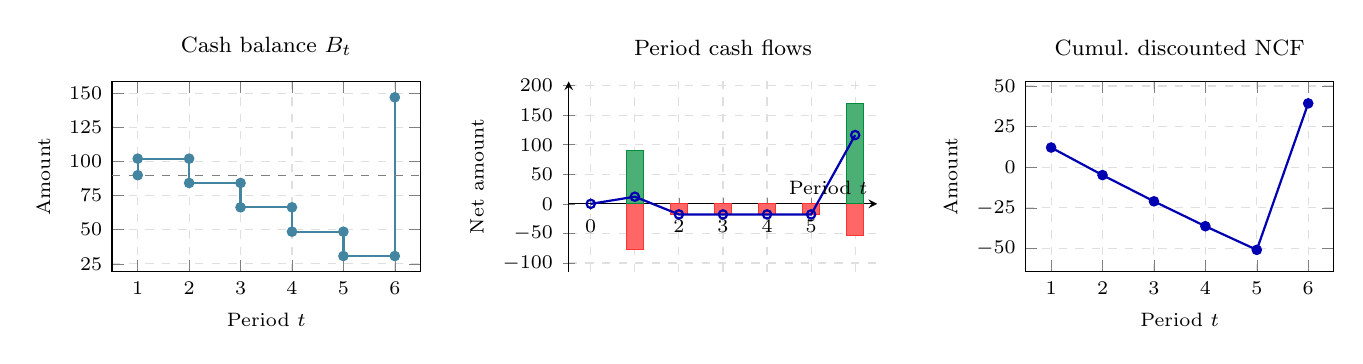
\begin{tikzpicture}[font=\footnotesize]
\begin{scope}
\begin{axis}[
    width=5.5cm, height=4.0cm,
    title={\footnotesize Cash balance $B_t$},
    xlabel={Period $t$}, ylabel={Amount},
    xmin=0.5, xmax=6.5,
    ymin=19.1, ymax=158.8,
    xtick={1,2,3,4,5,6},
    ytick={25,50,75,100,125,150},
    grid=major, grid style={dashed,gray!25},
    tick label style={font=\scriptsize},
    label style={font=\scriptsize}, title style={font=\scriptsize},
  ]
  \addplot[thick,cyan!60!black,mark=*,mark size=1.5pt] coordinates {(1,90) (1,102.143) (2,102.143) (2,84.286) (3,84.286) (3,66.429) (4,66.429) (4,48.572) (5,48.572) (5,30.715) (6,30.715) (6,147.143)};
  \draw[dashed,gray] (axis cs:0.5,90)--(axis cs:6.5,90) node[right,font=\tiny,gray] {$B_1$};
\end{axis}
\end{scope}

\begin{scope}[xshift=5.8cm]
\begin{axis}[
    width=5.5cm, height=4.0cm,
    title={\footnotesize Period cash flows},
    xlabel={Period $t$}, ylabel={Net amount},
    xmin=-0.5, xmax=6.5,
    ymin=-115.036, ymax=207.179,
    xtick={0,1,2,3,4,5,6},
    ytick={-100,-50,0,50,100,150,200},
    grid=major, grid style={dashed,gray!25},
    tick label style={font=\scriptsize},
    label style={font=\scriptsize}, title style={font=\scriptsize},
    axis x line=center, axis y line=left,
    clip=false,
  ]
  \addplot[ybar,bar width=0.22cm,fill=red!60,draw=red!80] coordinates {(1,-77.857) (2,-17.857) (3,-17.857) (4,-17.857) (5,-17.857) (6,-53.572)};
  \addplot[ybar,bar width=0.22cm,fill=msgreen!70,draw=msgreen] coordinates {(1,90) (6,170)};
  \addplot[thick,blue!70!black,mark=o,mark size=1.5pt] coordinates {(0,0) (1,12.143) (2,-17.857) (3,-17.857) (4,-17.857) (5,-17.857) (6,116.428)};
\end{axis}
\end{scope}

\begin{scope}[xshift=11.6cm]
\begin{axis}[
    width=5.5cm, height=4.0cm,
    title={\footnotesize Cumul.\ discounted NCF},
    xlabel={Period $t$}, ylabel={Amount},
    xmin=0.5, xmax=6.5,
    ymin=-64.306, ymax=52.811,
    xtick={1,2,3,4,5,6},
    ytick={-50,-25,0,25,50},
    grid=major, grid style={dashed,gray!25},
    tick label style={font=\scriptsize},
    label style={font=\scriptsize}, title style={font=\scriptsize},
  ]
  \addplot[thick,blue!70!black,mark=*,mark size=1.5pt] coordinates {(1,12.143) (2,-4.821) (3,-20.937) (4,-36.248) (5,-50.792) (6,39.298)};
\end{axis}
\end{scope}

\end{tikzpicture}
\caption{SP-M portfolio view. $Z^*=39.298$.}
\label{fig:spm_portfolio}
\end{figure}

\newpage

\subsection*{SP-Mp  (Group~G2)}
\begin{center}
\begin{tabular}{ll}
\toprule
$n$,\;$H$ & $2$,\;$6$ \\
$\BAC_i$ & $(60, 100)$ \\
$CP_i$   & $(90, 80)$ \\
$B_1,\;\gamma$ & $90,\;0.95$ \\
$Z^*$ & $30$ \\
Outcome & \texttt{good_completed} \\
\bottomrule
\end{tabular}
\end{center}

\paragraph{Project 1 timeline.}
\begin{center}
\begin{tabular}{rrrrrrrrrrl}
\toprule
$t$ & $x$ & $P$ & BCWS & BCWP & ACWP & SPI & CPI & $\tau$ & MS & $R_{\mathrm{net}}$\\
\midrule
1 & 60 & 1 & 0.5 & 1 & 1 & 2 & 1 & 2 & \texttt{1} & 90 \\
2 & 0 & 1 & 1 & 1 & 1 & 1 & 1 & 2 & \texttt{---} & 0 \\
\bottomrule
\end{tabular}
\end{center}
\paragraph{Project 2 timeline.}
\begin{center}
\begin{tabular}{rrrrrrrrrrl}
\toprule
$t$ & $x$ & $P$ & BCWS & BCWP & ACWP & SPI & CPI & $\tau$ & MS & $R_{\mathrm{net}}$\\
\midrule
1 & 0 & 0 & 0.125 & 0 & 0 & 0 & 1 & 2 & \texttt{---} & 0 \\
2 & 0 & 0 & 0.25 & 0 & 0 & 0 & 1 & 2 & \texttt{---} & 0 \\
3 & 0 & 0 & 0.375 & 0 & 0 & 0 & 1 & 2 & \texttt{---} & 0 \\
\bottomrule
\end{tabular}
\end{center}
\paragraph{Portfolio strip.}
\begin{center}
\begin{tabular}{rrrrrrr}
\toprule
$t$ & $B_t$ & $\Sigma\mathrm{In}$ & $\Sigma\mathrm{Out}$ & $\Sigma\mathrm{Net}$ & $\gamma^{t-1}\mathrm{Net}$ & $Z_t^{\mathrm{cum}}$\\
\midrule
1 & 120 & 90 & 60 & 30 & 30 & 30 \\
2 & 120 & 0 & 0 & 0 & 0 & 30 \\
3 & 120 & 0 & 0 & 0 & 0 & 30 \\
4 & 120 & 0 & 0 & 0 & 0 & 30 \\
5 & 120 & 0 & 0 & 0 & 0 & 30 \\
6 & 120 & 0 & 0 & 0 & 0 & 30 \\
\bottomrule
\end{tabular}
\end{center}

\begin{figure}[htbp]
\centering
% === Project 1 row for SP-Mp ===
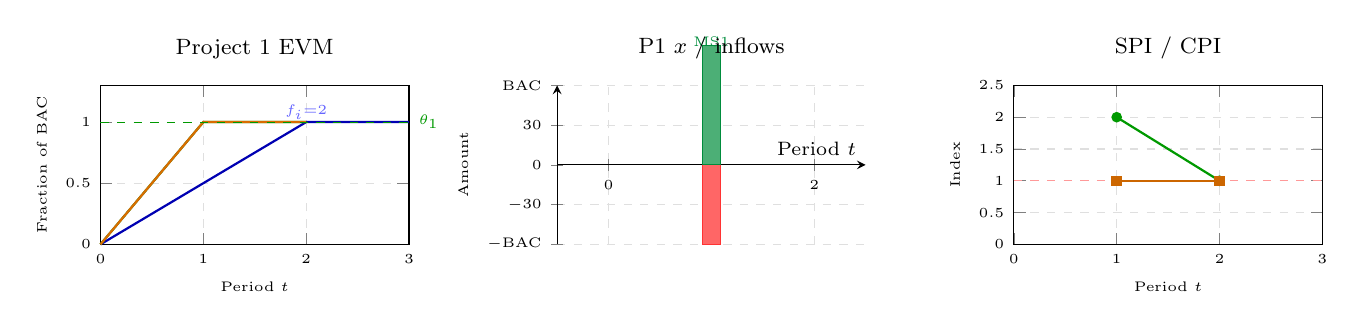
\begin{tikzpicture}[font=\footnotesize]
\begin{scope}
\begin{axis}[
    name=evmspmp_p1,
    width=5.5cm, height=3.6cm,
    title={\footnotesize Project 1 EVM},
    xlabel={Period $t$}, ylabel={Fraction of $\BAC$},
    xmin=0, xmax=3, ymin=0, ymax=1.30,
    xtick={0,1,2,3},
    ytick={0,0.5,1},
    grid=major, grid style={dashed,gray!25},
    tick label style={font=\tiny},
    label style={font=\tiny}, title style={font=\tiny},
    clip=false,
  ]
  \addplot[thick,blue!70!black] coordinates {(0,0) (1,0.5) (2,1) (3,1)};
  \addplot[thick,green!55!black] coordinates {(0,0) (1,1) (2,1)};
  \addplot[thick,orange!85!black] coordinates {(0,0) (1,1) (2,1)};
  \draw[green!60!black,dashed,thin] (axis cs:0,1)--(axis cs:3,1) node[right,green!60!black,font=\tiny] {$\theta_{1}$};
  \node[font=\tiny,blue!60] at (axis cs:2,1.08) {$f_i{=}2$};
\end{axis}
\end{scope}

\begin{scope}[xshift=5.8cm]
\begin{axis}[
    name=msspmp_p1,
    width=5.5cm, height=3.6cm,
    title={\footnotesize P1 $x$\ /\ inflows},
    xlabel={Period $t$}, ylabel={Amount},
    xmin=-0.5, xmax=2.5, ymin=-60, ymax=60,
    xtick={0,1,2},
    ytick={-60,-30,0,30,60},
    yticklabels={$-\BAC$,$-30$,$0$,$30$,$\BAC$},
    grid=major, grid style={dashed,gray!25},
    tick label style={font=\tiny},
    label style={font=\tiny}, title style={font=\tiny},
    axis x line=center, axis y line=left,
    clip=false,
  ]
  \addplot[ybar,bar width=0.22cm,fill=red!60,draw=red!80] coordinates {(1,-60)};
  \addplot[ybar,bar width=0.22cm,fill=msgreen!70,draw=msgreen] coordinates {(1,90)};
  \node[font=\tiny,msgreen] at (axis cs:1,93) {MS1};
\end{axis}
\end{scope}

\begin{scope}[xshift=11.6cm]
\begin{axis}[
    name=spicpispmp_p1,
    width=5.5cm, height=3.6cm,
    title={\footnotesize SPI / CPI},
    xlabel={Period $t$}, ylabel={Index},
    xmin=0, xmax=3, ymin=0, ymax=2.5,
    xtick={0,1,2,3},
    ytick={0,0.5,1,1.5,2,2.5},
    grid=major, grid style={dashed,gray!25},
    tick label style={font=\tiny},
    label style={font=\tiny}, title style={font=\tiny},
    clip=false,
  ]
  \draw[red!40,dashed,thin] (axis cs:0,1)--(axis cs:3,1);
  \addplot[thick,green!60!black,mark=*,mark size=1.5pt] coordinates {(1,2) (2,1)};
  \addplot[thick,orange!80!black,mark=square*,mark size=1.5pt] coordinates {(1,1) (2,1)};
\end{axis}
\end{scope}

\end{tikzpicture}
\vspace{0.3cm}

% === Project 2 row for SP-Mp ===
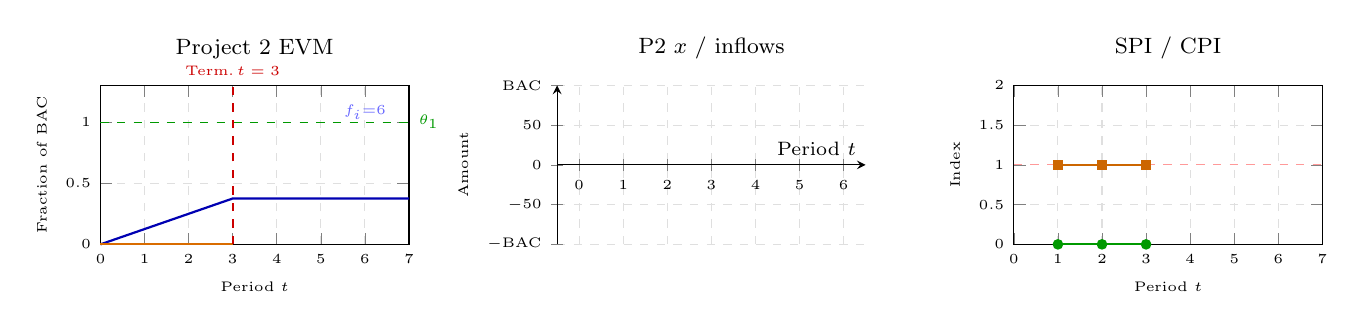
\begin{tikzpicture}[font=\footnotesize]
\begin{scope}
\begin{axis}[
    name=evmspmp_p2,
    width=5.5cm, height=3.6cm,
    title={\footnotesize Project 2 EVM},
    xlabel={Period $t$}, ylabel={Fraction of $\BAC$},
    xmin=0, xmax=7, ymin=0, ymax=1.30,
    xtick={0,1,2,3,4,5,6,7},
    ytick={0,0.5,1},
    grid=major, grid style={dashed,gray!25},
    tick label style={font=\tiny},
    label style={font=\tiny}, title style={font=\tiny},
    clip=false,
  ]
  \addplot[thick,blue!70!black] coordinates {(0,0) (1,0.125) (2,0.25) (3,0.375) (7,0.375)};
  \addplot[thick,green!55!black] coordinates {(0,0) (1,0) (2,0) (3,0)};
  \addplot[thick,orange!85!black] coordinates {(0,0) (1,0) (2,0) (3,0)};
  \draw[green!60!black,dashed,thin] (axis cs:0,1)--(axis cs:7,1) node[right,green!60!black,font=\tiny] {$\theta_{1}$};
  \node[font=\tiny,blue!60] at (axis cs:6,1.08) {$f_i{=}6$};
  \draw[red!80!black,dashed,thick] (axis cs:3,0)--(axis cs:3,1.30) node[above,font=\tiny,red!80!black] {Term.\,$t=3$};
\end{axis}
\end{scope}

\begin{scope}[xshift=5.8cm]
\begin{axis}[
    name=msspmp_p2,
    width=5.5cm, height=3.6cm,
    title={\footnotesize P2 $x$\ /\ inflows},
    xlabel={Period $t$}, ylabel={Amount},
    xmin=-0.5, xmax=6.5, ymin=-100, ymax=100,
    xtick={0,1,2,3,4,5,6},
    ytick={-100,-50,0,50,100},
    yticklabels={$-\BAC$,$-50$,$0$,$50$,$\BAC$},
    grid=major, grid style={dashed,gray!25},
    tick label style={font=\tiny},
    label style={font=\tiny}, title style={font=\tiny},
    axis x line=center, axis y line=left,
    clip=false,
  ]
\end{axis}
\end{scope}

\begin{scope}[xshift=11.6cm]
\begin{axis}[
    name=spicpispmp_p2,
    width=5.5cm, height=3.6cm,
    title={\footnotesize SPI / CPI},
    xlabel={Period $t$}, ylabel={Index},
    xmin=0, xmax=7, ymin=0, ymax=2,
    xtick={0,1,2,3,4,5,6,7},
    ytick={0,0.5,1,1.5,2},
    grid=major, grid style={dashed,gray!25},
    tick label style={font=\tiny},
    label style={font=\tiny}, title style={font=\tiny},
    clip=false,
  ]
  \draw[red!40,dashed,thin] (axis cs:0,1)--(axis cs:7,1);
  \addplot[thick,green!60!black,mark=*,mark size=1.5pt] coordinates {(1,0) (2,0) (3,0)};
  \addplot[thick,orange!80!black,mark=square*,mark size=1.5pt] coordinates {(1,1) (2,1) (3,1)};
\end{axis}
\end{scope}

\end{tikzpicture}

\caption{SP-Mp project view (2-project). Outcome: \texttt{good_completed}. $Z^*=30$.}
\label{fig:spmp_project}
\end{figure}

\begin{figure}[htbp]
\centering
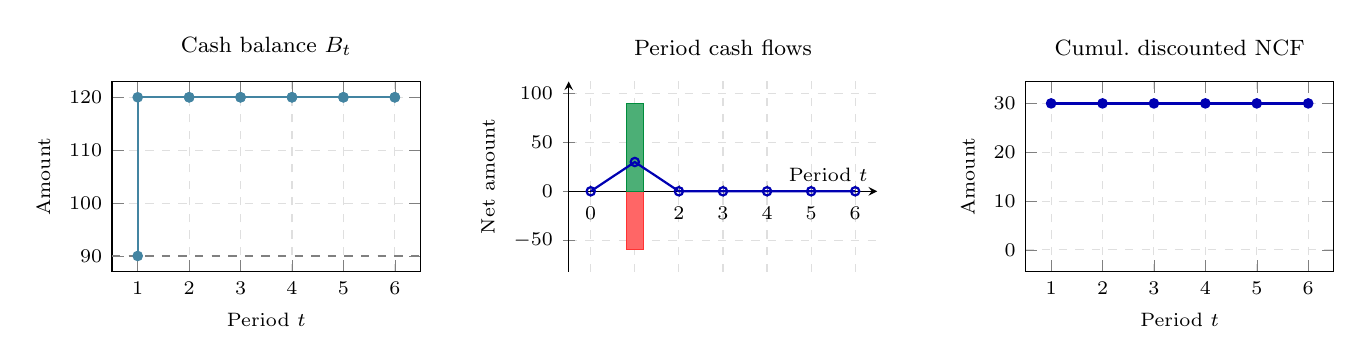
\begin{tikzpicture}[font=\footnotesize]
\begin{scope}
\begin{axis}[
    width=5.5cm, height=4.0cm,
    title={\footnotesize Cash balance $B_t$},
    xlabel={Period $t$}, ylabel={Amount},
    xmin=0.5, xmax=6.5,
    ymin=87, ymax=123,
    xtick={1,2,3,4,5,6},
    ytick={90,100,110,120},
    grid=major, grid style={dashed,gray!25},
    tick label style={font=\scriptsize},
    label style={font=\scriptsize}, title style={font=\scriptsize},
  ]
  \addplot[thick,cyan!60!black,mark=*,mark size=1.5pt] coordinates {(1,90) (1,120) (2,120) (2,120) (3,120) (3,120) (4,120) (4,120) (5,120) (5,120) (6,120) (6,120)};
  \draw[dashed,gray] (axis cs:0.5,90)--(axis cs:6.5,90) node[right,font=\tiny,gray] {$B_1$};
\end{axis}
\end{scope}

\begin{scope}[xshift=5.8cm]
\begin{axis}[
    width=5.5cm, height=4.0cm,
    title={\footnotesize Period cash flows},
    xlabel={Period $t$}, ylabel={Net amount},
    xmin=-0.5, xmax=6.5,
    ymin=-82.5, ymax=112.5,
    xtick={0,1,2,3,4,5,6},
    ytick={-50,0,50,100},
    grid=major, grid style={dashed,gray!25},
    tick label style={font=\scriptsize},
    label style={font=\scriptsize}, title style={font=\scriptsize},
    axis x line=center, axis y line=left,
    clip=false,
  ]
  \addplot[ybar,bar width=0.22cm,fill=red!60,draw=red!80] coordinates {(1,-60)};
  \addplot[ybar,bar width=0.22cm,fill=msgreen!70,draw=msgreen] coordinates {(1,90)};
  \addplot[thick,blue!70!black,mark=o,mark size=1.5pt] coordinates {(0,0) (1,30) (2,0) (3,0) (4,0) (5,0) (6,0)};
\end{axis}
\end{scope}

\begin{scope}[xshift=11.6cm]
\begin{axis}[
    width=5.5cm, height=4.0cm,
    title={\footnotesize Cumul.\ discounted NCF},
    xlabel={Period $t$}, ylabel={Amount},
    xmin=0.5, xmax=6.5,
    ymin=-4.5, ymax=34.5,
    xtick={1,2,3,4,5,6},
    ytick={0,10,20,30},
    grid=major, grid style={dashed,gray!25},
    tick label style={font=\scriptsize},
    label style={font=\scriptsize}, title style={font=\scriptsize},
  ]
  \addplot[thick,blue!70!black,mark=*,mark size=1.5pt] coordinates {(1,30) (2,30) (3,30) (4,30) (5,30) (6,30)};
\end{axis}
\end{scope}

\end{tikzpicture}
\caption{SP-Mp portfolio view. $Z^*=30$.}
\label{fig:spmp_portfolio}
\end{figure}

\newpage


\subsection*{Group 3: Advance Payments and Recovery}

\subsection*{SP-2  (Group~G3)}
\begin{center}
\begin{tabular}{ll}
\toprule
$n$,\;$H$ & $1$,\;$6$ \\
$\BAC,\;CP$ & $100,\;100$ \\
$s_i,\;f_i,\;D^{\mathrm{plan}}$ & $1,\;6,\;6$ \\
$\bar\eta$ & $1$ \\
$\alpha,\;A$ & $0.3,\;30$ \\
$M,\;\theta$ & $2,\;(0.5,1)$ \\
$\phi,\;e_{i,j}$ & $(0.5,0.5),\;(1,4)$ \\
$\mu,\;\Omega,\;\tau^{\mathrm{tol}}$ & $0.05,\;1,\;1$ \\
$B_1,\;\gamma$ & $300,\;0.95$ \\
$Z^*$ & $1.5$ \\
Outcome & \texttt{terminated} \\
\bottomrule
\end{tabular}
\end{center}

\begin{center}
\begin{tabular}{rrrrrrrrrrl}
\toprule
$t$ & $x$ & $P$ & BCWS & BCWP & ACWP & SPI & CPI & $\tau$ & MS & $R_{\mathrm{net}}$\\
\midrule
1 & 0 & 0 & 0.167 & 0 & 0 & 0 & 1 & 1 & \texttt{---} & 0 \\
2 & 0 & 0 & 0.333 & 0 & 0 & 0 & 1 & 1 & \texttt{---} & -30 \\
\bottomrule
\end{tabular}
\end{center}
\paragraph{Portfolio strip.}
\begin{center}
\begin{tabular}{rrrrrrr}
\toprule
$t$ & $B_t$ & $\Sigma\mathrm{In}$ & $\Sigma\mathrm{Out}$ & $\Sigma\mathrm{Net}$ & $\gamma^{t-1}\mathrm{Net}$ & $Z_t^{\mathrm{cum}}$\\
\midrule
1 & 330 & 0 & 0 & 0 & 0 & 30 \\
2 & 300 & -30 & 0 & -30 & -28.5 & 1.5 \\
3 & 300 & 0 & 0 & 0 & 0 & 1.5 \\
4 & 300 & 0 & 0 & 0 & 0 & 1.5 \\
5 & 300 & 0 & 0 & 0 & 0 & 1.5 \\
6 & 300 & 0 & 0 & 0 & 0 & 1.5 \\
\bottomrule
\end{tabular}
\end{center}

\begin{figure}[htbp]
\centering
% === Project 1 row for SP-2 ===
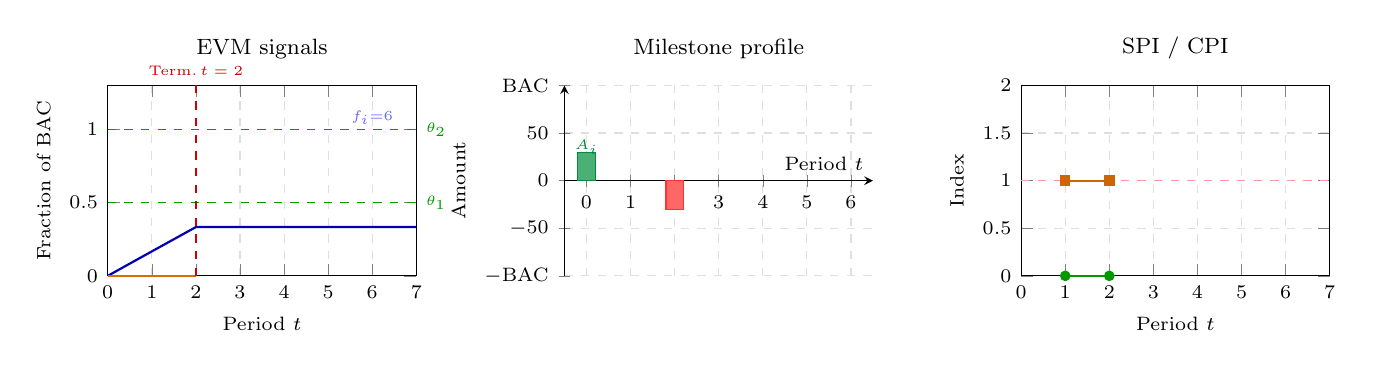
\begin{tikzpicture}[font=\footnotesize]
\begin{scope}
\begin{axis}[
    name=evmsp2_p1,
    width=5.5cm, height=4.0cm,
    title={\footnotesize EVM signals},
    xlabel={Period $t$}, ylabel={Fraction of $\BAC$},
    xmin=0, xmax=7, ymin=0, ymax=1.30,
    xtick={0,1,2,3,4,5,6,7},
    ytick={0,0.5,1},
    grid=major, grid style={dashed,gray!25},
    tick label style={font=\scriptsize},
    label style={font=\scriptsize}, title style={font=\scriptsize},
    clip=false,
  ]
  \addplot[thick,blue!70!black] coordinates {(0,0) (1,0.167) (2,0.333) (7,0.333)};
  \addplot[thick,green!55!black] coordinates {(0,0) (1,0) (2,0)};
  \addplot[thick,orange!85!black] coordinates {(0,0) (1,0) (2,0)};
  \draw[green!60!black,dashed,thin] (axis cs:0,0.5)--(axis cs:7,0.5) node[right,green!60!black,font=\tiny] {$\theta_{1}$};
  \draw[green!60!black,dashed,thin] (axis cs:0,1)--(axis cs:7,1) node[right,green!60!black,font=\tiny] {$\theta_{2}$};
  \node[font=\tiny,blue!60] at (axis cs:6,1.08) {$f_i{=}6$};
  \draw[red!80!black,dashed,thick] (axis cs:2,0)--(axis cs:2,1.30) node[above,font=\tiny,red!80!black] {Term.\,$t=2$};
\end{axis}
\end{scope}

\begin{scope}[xshift=5.8cm]
\begin{axis}[
    name=mssp2_p1,
    width=5.5cm, height=4.0cm,
    title={\footnotesize Milestone profile},
    xlabel={Period $t$}, ylabel={Amount},
    xmin=-0.5, xmax=6.5, ymin=-100, ymax=100,
    xtick={0,1,2,3,4,5,6},
    ytick={-100,-50,0,50,100},
    yticklabels={$-\BAC$,$-50$,$0$,$50$,$\BAC$},
    grid=major, grid style={dashed,gray!25},
    tick label style={font=\scriptsize},
    label style={font=\scriptsize}, title style={font=\scriptsize},
    axis x line=center, axis y line=left,
    clip=false,
  ]
  \addplot[ybar,bar width=0.22cm,fill=red!60,draw=red!80] coordinates {(2,-30)};
  \addplot[ybar,bar width=0.22cm,fill=msgreen!70,draw=msgreen] coordinates {(0,30)};
  \node[font=\tiny,msgreen] at (axis cs:0,35) {$A_i$};
\end{axis}
\end{scope}

\begin{scope}[xshift=11.6cm]
\begin{axis}[
    name=spicpisp2_p1,
    width=5.5cm, height=4.0cm,
    title={\footnotesize SPI / CPI},
    xlabel={Period $t$}, ylabel={Index},
    xmin=0, xmax=7, ymin=0, ymax=2,
    xtick={0,1,2,3,4,5,6,7},
    ytick={0,0.5,1,1.5,2},
    grid=major, grid style={dashed,gray!25},
    tick label style={font=\scriptsize},
    label style={font=\scriptsize}, title style={font=\scriptsize},
    clip=false,
  ]
  \draw[red!40,dashed,thin] (axis cs:0,1)--(axis cs:7,1);
  \addplot[thick,green!60!black,mark=*,mark size=1.5pt] coordinates {(1,0) (2,0)};
  \addplot[thick,orange!80!black,mark=square*,mark size=1.5pt] coordinates {(1,1) (2,1)};
\end{axis}
\end{scope}

\end{tikzpicture}

\caption{SP-2 project view (single-project). Outcome: \texttt{terminated}. $Z^*=1.5$.}
\label{fig:sp2_project}
\end{figure}

\begin{figure}[htbp]
\centering
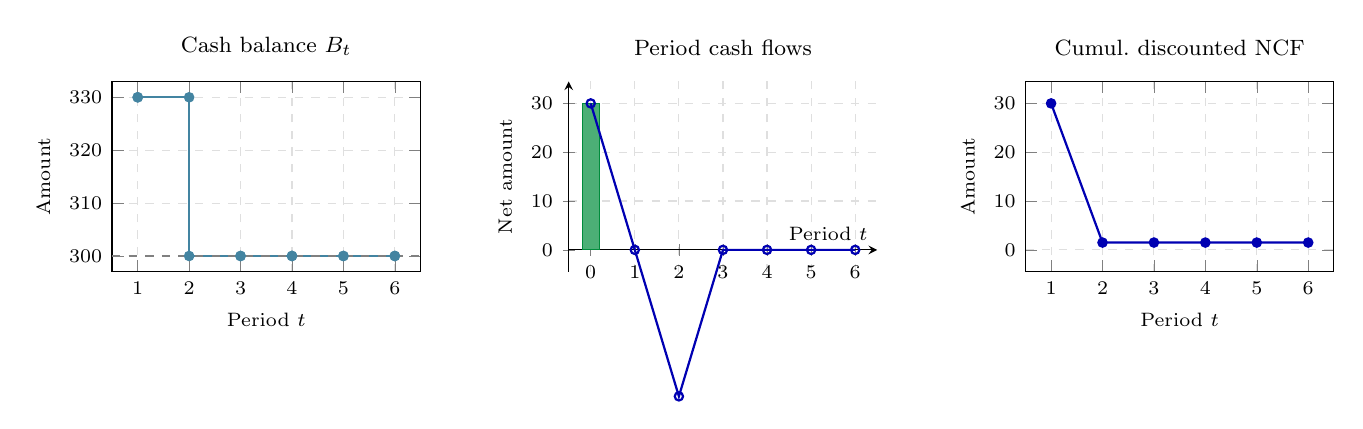
\begin{tikzpicture}[font=\footnotesize]
\begin{scope}
\begin{axis}[
    width=5.5cm, height=4.0cm,
    title={\footnotesize Cash balance $B_t$},
    xlabel={Period $t$}, ylabel={Amount},
    xmin=0.5, xmax=6.5,
    ymin=297, ymax=333,
    xtick={1,2,3,4,5,6},
    ytick={300,310,320,330},
    grid=major, grid style={dashed,gray!25},
    tick label style={font=\scriptsize},
    label style={font=\scriptsize}, title style={font=\scriptsize},
  ]
  \addplot[thick,cyan!60!black,mark=*,mark size=1.5pt] coordinates {(1,330) (1,330) (2,330) (2,300) (3,300) (3,300) (4,300) (4,300) (5,300) (5,300) (6,300) (6,300)};
  \draw[dashed,gray] (axis cs:0.5,300)--(axis cs:6.5,300) node[right,font=\tiny,gray] {$B_1$};
\end{axis}
\end{scope}

\begin{scope}[xshift=5.8cm]
\begin{axis}[
    width=5.5cm, height=4.0cm,
    title={\footnotesize Period cash flows},
    xlabel={Period $t$}, ylabel={Net amount},
    xmin=-0.5, xmax=6.5,
    ymin=-4.5, ymax=34.5,
    xtick={0,1,2,3,4,5,6},
    ytick={0,10,20,30},
    grid=major, grid style={dashed,gray!25},
    tick label style={font=\scriptsize},
    label style={font=\scriptsize}, title style={font=\scriptsize},
    axis x line=center, axis y line=left,
    clip=false,
  ]
  \addplot[ybar,bar width=0.22cm,fill=msgreen!70,draw=msgreen] coordinates {(0,30)};
  \addplot[thick,blue!70!black,mark=o,mark size=1.5pt] coordinates {(0,30) (1,0) (2,-30) (3,0) (4,0) (5,0) (6,0)};
\end{axis}
\end{scope}

\begin{scope}[xshift=11.6cm]
\begin{axis}[
    width=5.5cm, height=4.0cm,
    title={\footnotesize Cumul.\ discounted NCF},
    xlabel={Period $t$}, ylabel={Amount},
    xmin=0.5, xmax=6.5,
    ymin=-4.5, ymax=34.5,
    xtick={1,2,3,4,5,6},
    ytick={0,10,20,30},
    grid=major, grid style={dashed,gray!25},
    tick label style={font=\scriptsize},
    label style={font=\scriptsize}, title style={font=\scriptsize},
  ]
  \addplot[thick,blue!70!black,mark=*,mark size=1.5pt] coordinates {(1,30) (2,1.5) (3,1.5) (4,1.5) (5,1.5) (6,1.5)};
\end{axis}
\end{scope}

\end{tikzpicture}
\caption{SP-2 portfolio view. $Z^*=1.5$.}
\label{fig:sp2_portfolio}
\end{figure}

\newpage

\subsection*{SP-2a  (Group~G3)}
\begin{center}
\begin{tabular}{ll}
\toprule
$n$,\;$H$ & $1$,\;$4$ \\
$\BAC,\;CP$ & $100,\;120$ \\
$s_i,\;f_i,\;D^{\mathrm{plan}}$ & $1,\;4,\;4$ \\
$\bar\eta$ & $1$ \\
$\alpha,\;A$ & $0.3,\;30$ \\
$M,\;\theta$ & $1,\;(1)$ \\
$\phi,\;e_{i,j}$ & $(1),\;(1)$ \\
$\mu,\;\Omega,\;\tau^{\mathrm{tol}}$ & $0.3,\;1,\;1$ \\
$B_1,\;\gamma$ & $300,\;0.95$ \\
$Z^*$ & $20.5$ \\
Outcome & \texttt{completed} \\
\bottomrule
\end{tabular}
\end{center}

\begin{center}
\begin{tabular}{rrrrrrrrrrl}
\toprule
$t$ & $x$ & $P$ & BCWS & BCWP & ACWP & SPI & CPI & $\tau$ & MS & $R_{\mathrm{net}}$\\
\midrule
1 & 100 & 1 & 0.25 & 1 & 1 & 4 & 1 & 1 & \texttt{1} & 90 \\
2 & 0 & 1 & 0.5 & 1 & 1 & 2 & 1 & 1 & \texttt{---} & 0 \\
3 & 0 & 1 & 0.75 & 1 & 1 & 1.333 & 1 & 1 & \texttt{---} & 0 \\
4 & 0 & 1 & 1 & 1 & 1 & 1 & 1 & 1 & \texttt{---} & 0 \\
\bottomrule
\end{tabular}
\end{center}
\paragraph{Portfolio strip.}
\begin{center}
\begin{tabular}{rrrrrrr}
\toprule
$t$ & $B_t$ & $\Sigma\mathrm{In}$ & $\Sigma\mathrm{Out}$ & $\Sigma\mathrm{Net}$ & $\gamma^{t-1}\mathrm{Net}$ & $Z_t^{\mathrm{cum}}$\\
\midrule
1 & 320 & 90 & 100 & -10 & -10 & 20 \\
2 & 320 & 0 & 0 & 0 & 0 & 20 \\
3 & 320 & 0 & 0 & 0 & 0 & 20 \\
4 & 320 & 0 & 0 & 0 & 0 & 20 \\
\bottomrule
\end{tabular}
\end{center}

\begin{figure}[htbp]
\centering
% === Project 1 row for SP-2a ===
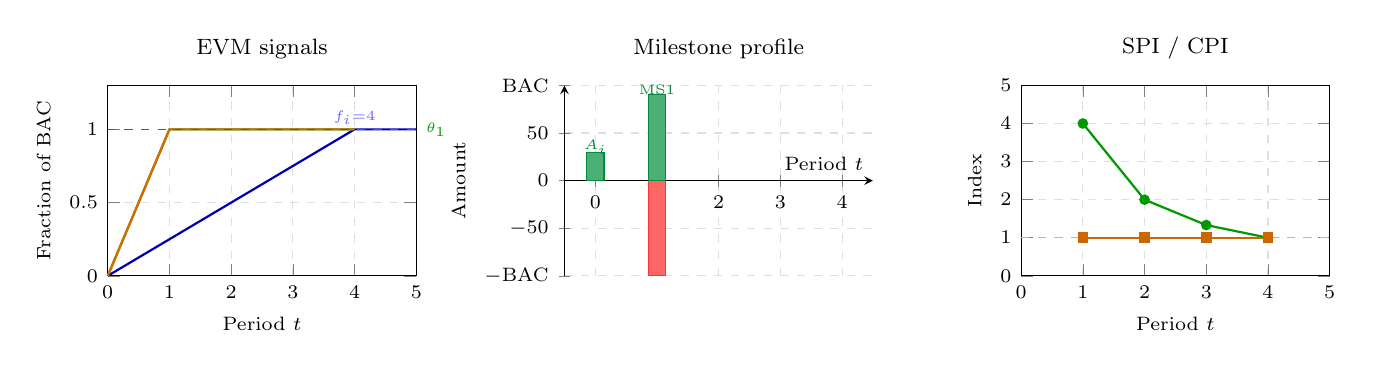
\begin{tikzpicture}[font=\footnotesize]
\begin{scope}
\begin{axis}[
    name=evmsp2a_p1,
    width=5.5cm, height=4.0cm,
    title={\footnotesize EVM signals},
    xlabel={Period $t$}, ylabel={Fraction of $\BAC$},
    xmin=0, xmax=5, ymin=0, ymax=1.30,
    xtick={0,1,2,3,4,5},
    ytick={0,0.5,1},
    grid=major, grid style={dashed,gray!25},
    tick label style={font=\scriptsize},
    label style={font=\scriptsize}, title style={font=\scriptsize},
    clip=false,
  ]
  \addplot[thick,blue!70!black] coordinates {(0,0) (1,0.25) (2,0.5) (3,0.75) (4,1) (5,1)};
  \addplot[thick,green!55!black] coordinates {(0,0) (1,1) (2,1) (3,1) (4,1)};
  \addplot[thick,orange!85!black] coordinates {(0,0) (1,1) (2,1) (3,1) (4,1)};
  \draw[green!60!black,dashed,thin] (axis cs:0,1)--(axis cs:5,1) node[right,green!60!black,font=\tiny] {$\theta_{1}$};
  \node[font=\tiny,blue!60] at (axis cs:4,1.08) {$f_i{=}4$};
\end{axis}
\end{scope}

\begin{scope}[xshift=5.8cm]
\begin{axis}[
    name=mssp2a_p1,
    width=5.5cm, height=4.0cm,
    title={\footnotesize Milestone profile},
    xlabel={Period $t$}, ylabel={Amount},
    xmin=-0.5, xmax=4.5, ymin=-100, ymax=100,
    xtick={0,1,2,3,4},
    ytick={-100,-50,0,50,100},
    yticklabels={$-\BAC$,$-50$,$0$,$50$,$\BAC$},
    grid=major, grid style={dashed,gray!25},
    tick label style={font=\scriptsize},
    label style={font=\scriptsize}, title style={font=\scriptsize},
    axis x line=center, axis y line=left,
    clip=false,
  ]
  \addplot[ybar,bar width=0.22cm,fill=red!60,draw=red!80] coordinates {(1,-100)};
  \addplot[ybar,bar width=0.22cm,fill=msgreen!70,draw=msgreen] coordinates {(0,30) (1,90)};
  \node[font=\tiny,msgreen] at (axis cs:1,95) {MS1};
  \node[font=\tiny,msgreen] at (axis cs:0,35) {$A_i$};
\end{axis}
\end{scope}

\begin{scope}[xshift=11.6cm]
\begin{axis}[
    name=spicpisp2a_p1,
    width=5.5cm, height=4.0cm,
    title={\footnotesize SPI / CPI},
    xlabel={Period $t$}, ylabel={Index},
    xmin=0, xmax=5, ymin=0, ymax=5,
    xtick={0,1,2,3,4,5},
    ytick={0,1,2,3,4,5},
    grid=major, grid style={dashed,gray!25},
    tick label style={font=\scriptsize},
    label style={font=\scriptsize}, title style={font=\scriptsize},
    clip=false,
  ]
  \draw[red!40,dashed,thin] (axis cs:0,1)--(axis cs:5,1);
  \addplot[thick,green!60!black,mark=*,mark size=1.5pt] coordinates {(1,4) (2,2) (3,1.333) (4,1)};
  \addplot[thick,orange!80!black,mark=square*,mark size=1.5pt] coordinates {(1,1) (2,1) (3,1) (4,1)};
\end{axis}
\end{scope}

\end{tikzpicture}

\caption{SP-2a project view (single-project). Outcome: \texttt{completed}. $Z^*=20.5$.}
\label{fig:sp2a_project}
\end{figure}

\begin{figure}[htbp]
\centering
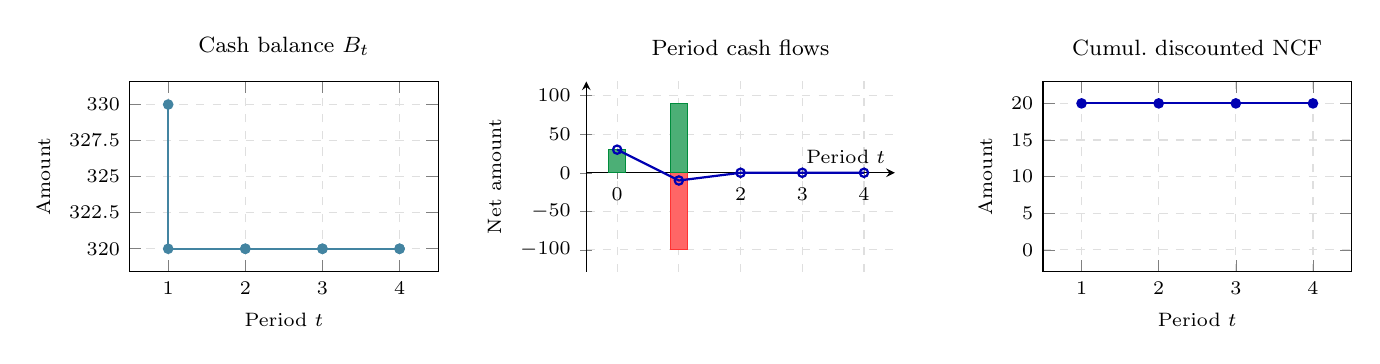
\begin{tikzpicture}[font=\footnotesize]
\begin{scope}
\begin{axis}[
    width=5.5cm, height=4.0cm,
    title={\footnotesize Cash balance $B_t$},
    xlabel={Period $t$}, ylabel={Amount},
    xmin=0.5, xmax=4.5,
    ymin=318.4, ymax=331.6,
    xtick={1,2,3,4},
    ytick={320,322.5,325,327.5,330},
    grid=major, grid style={dashed,gray!25},
    tick label style={font=\scriptsize},
    label style={font=\scriptsize}, title style={font=\scriptsize},
  ]
  \addplot[thick,cyan!60!black,mark=*,mark size=1.5pt] coordinates {(1,330) (1,320) (2,320) (2,320) (3,320) (3,320) (4,320) (4,320)};
  \draw[dashed,gray] (axis cs:0.5,300)--(axis cs:4.5,300) node[right,font=\tiny,gray] {$B_1$};
\end{axis}
\end{scope}

\begin{scope}[xshift=5.8cm]
\begin{axis}[
    width=5.5cm, height=4.0cm,
    title={\footnotesize Period cash flows},
    xlabel={Period $t$}, ylabel={Net amount},
    xmin=-0.5, xmax=4.5,
    ymin=-128.5, ymax=118.5,
    xtick={0,1,2,3,4},
    ytick={-100,-50,0,50,100},
    grid=major, grid style={dashed,gray!25},
    tick label style={font=\scriptsize},
    label style={font=\scriptsize}, title style={font=\scriptsize},
    axis x line=center, axis y line=left,
    clip=false,
  ]
  \addplot[ybar,bar width=0.22cm,fill=red!60,draw=red!80] coordinates {(1,-100)};
  \addplot[ybar,bar width=0.22cm,fill=msgreen!70,draw=msgreen] coordinates {(0,30) (1,90)};
  \addplot[thick,blue!70!black,mark=o,mark size=1.5pt] coordinates {(0,30) (1,-10) (2,0) (3,0) (4,0)};
\end{axis}
\end{scope}

\begin{scope}[xshift=11.6cm]
\begin{axis}[
    width=5.5cm, height=4.0cm,
    title={\footnotesize Cumul.\ discounted NCF},
    xlabel={Period $t$}, ylabel={Amount},
    xmin=0.5, xmax=4.5,
    ymin=-3, ymax=23,
    xtick={1,2,3,4},
    ytick={0,5,10,15,20},
    grid=major, grid style={dashed,gray!25},
    tick label style={font=\scriptsize},
    label style={font=\scriptsize}, title style={font=\scriptsize},
  ]
  \addplot[thick,blue!70!black,mark=*,mark size=1.5pt] coordinates {(1,20) (2,20) (3,20) (4,20)};
\end{axis}
\end{scope}

\end{tikzpicture}
\caption{SP-2a portfolio view. $Z^*=20.5$.}
\label{fig:sp2a_portfolio}
\end{figure}

\newpage

\subsection*{SP-2b  (Group~G3)}
\begin{center}
\begin{tabular}{ll}
\toprule
$n$,\;$H$ & $1$,\;$4$ \\
$\BAC,\;CP$ & $100,\;60$ \\
$s_i,\;f_i,\;D^{\mathrm{plan}}$ & $1,\;4,\;4$ \\
$\bar\eta$ & $1$ \\
$\alpha,\;A$ & $0.3,\;30$ \\
$M,\;\theta$ & $1,\;(1)$ \\
$\phi,\;e_{i,j}$ & $(1),\;(1)$ \\
$\mu,\;\Omega,\;\tau^{\mathrm{tol}}$ & $0.3,\;1,\;1$ \\
$B_1,\;\gamma$ & $300,\;0.95$ \\
$Z^*$ & $1.5$ \\
Outcome & \texttt{terminated} \\
\bottomrule
\end{tabular}
\end{center}

\begin{center}
\begin{tabular}{rrrrrrrrrrl}
\toprule
$t$ & $x$ & $P$ & BCWS & BCWP & ACWP & SPI & CPI & $\tau$ & MS & $R_{\mathrm{net}}$\\
\midrule
1 & 0 & 0 & 0.25 & 0 & 0 & 0 & 1 & 1 & \texttt{---} & 0 \\
2 & 0 & 0 & 0.5 & 0 & 0 & 0 & 1 & 1 & \texttt{---} & -30 \\
\bottomrule
\end{tabular}
\end{center}
\paragraph{Portfolio strip.}
\begin{center}
\begin{tabular}{rrrrrrr}
\toprule
$t$ & $B_t$ & $\Sigma\mathrm{In}$ & $\Sigma\mathrm{Out}$ & $\Sigma\mathrm{Net}$ & $\gamma^{t-1}\mathrm{Net}$ & $Z_t^{\mathrm{cum}}$\\
\midrule
1 & 330 & 0 & 0 & 0 & 0 & 30 \\
2 & 300 & -30 & 0 & -30 & -28.5 & 1.5 \\
3 & 300 & 0 & 0 & 0 & 0 & 1.5 \\
4 & 300 & 0 & 0 & 0 & 0 & 1.5 \\
\bottomrule
\end{tabular}
\end{center}

\begin{figure}[htbp]
\centering
% === Project 1 row for SP-2b ===
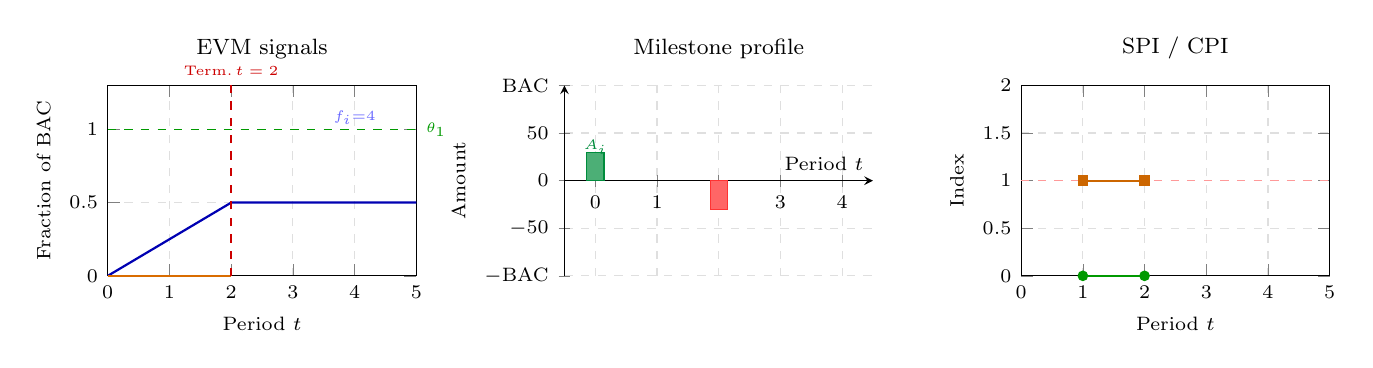
\begin{tikzpicture}[font=\footnotesize]
\begin{scope}
\begin{axis}[
    name=evmsp2b_p1,
    width=5.5cm, height=4.0cm,
    title={\footnotesize EVM signals},
    xlabel={Period $t$}, ylabel={Fraction of $\BAC$},
    xmin=0, xmax=5, ymin=0, ymax=1.30,
    xtick={0,1,2,3,4,5},
    ytick={0,0.5,1},
    grid=major, grid style={dashed,gray!25},
    tick label style={font=\scriptsize},
    label style={font=\scriptsize}, title style={font=\scriptsize},
    clip=false,
  ]
  \addplot[thick,blue!70!black] coordinates {(0,0) (1,0.25) (2,0.5) (5,0.5)};
  \addplot[thick,green!55!black] coordinates {(0,0) (1,0) (2,0)};
  \addplot[thick,orange!85!black] coordinates {(0,0) (1,0) (2,0)};
  \draw[green!60!black,dashed,thin] (axis cs:0,1)--(axis cs:5,1) node[right,green!60!black,font=\tiny] {$\theta_{1}$};
  \node[font=\tiny,blue!60] at (axis cs:4,1.08) {$f_i{=}4$};
  \draw[red!80!black,dashed,thick] (axis cs:2,0)--(axis cs:2,1.30) node[above,font=\tiny,red!80!black] {Term.\,$t=2$};
\end{axis}
\end{scope}

\begin{scope}[xshift=5.8cm]
\begin{axis}[
    name=mssp2b_p1,
    width=5.5cm, height=4.0cm,
    title={\footnotesize Milestone profile},
    xlabel={Period $t$}, ylabel={Amount},
    xmin=-0.5, xmax=4.5, ymin=-100, ymax=100,
    xtick={0,1,2,3,4},
    ytick={-100,-50,0,50,100},
    yticklabels={$-\BAC$,$-50$,$0$,$50$,$\BAC$},
    grid=major, grid style={dashed,gray!25},
    tick label style={font=\scriptsize},
    label style={font=\scriptsize}, title style={font=\scriptsize},
    axis x line=center, axis y line=left,
    clip=false,
  ]
  \addplot[ybar,bar width=0.22cm,fill=red!60,draw=red!80] coordinates {(2,-30)};
  \addplot[ybar,bar width=0.22cm,fill=msgreen!70,draw=msgreen] coordinates {(0,30)};
  \node[font=\tiny,msgreen] at (axis cs:0,35) {$A_i$};
\end{axis}
\end{scope}

\begin{scope}[xshift=11.6cm]
\begin{axis}[
    name=spicpisp2b_p1,
    width=5.5cm, height=4.0cm,
    title={\footnotesize SPI / CPI},
    xlabel={Period $t$}, ylabel={Index},
    xmin=0, xmax=5, ymin=0, ymax=2,
    xtick={0,1,2,3,4,5},
    ytick={0,0.5,1,1.5,2},
    grid=major, grid style={dashed,gray!25},
    tick label style={font=\scriptsize},
    label style={font=\scriptsize}, title style={font=\scriptsize},
    clip=false,
  ]
  \draw[red!40,dashed,thin] (axis cs:0,1)--(axis cs:5,1);
  \addplot[thick,green!60!black,mark=*,mark size=1.5pt] coordinates {(1,0) (2,0)};
  \addplot[thick,orange!80!black,mark=square*,mark size=1.5pt] coordinates {(1,1) (2,1)};
\end{axis}
\end{scope}

\end{tikzpicture}

\caption{SP-2b project view (single-project). Outcome: \texttt{terminated}. $Z^*=1.5$.}
\label{fig:sp2b_project}
\end{figure}

\begin{figure}[htbp]
\centering
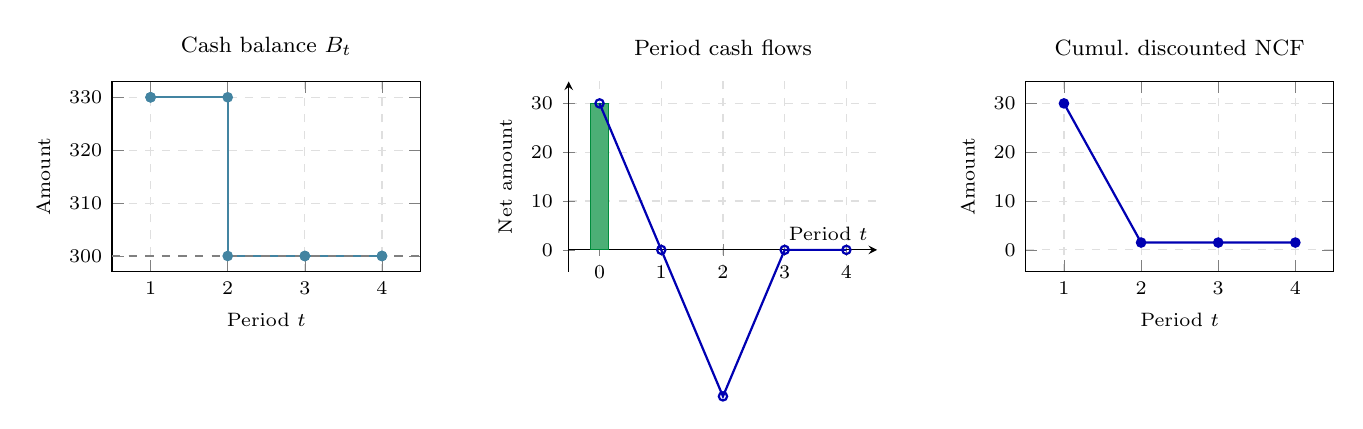
\begin{tikzpicture}[font=\footnotesize]
\begin{scope}
\begin{axis}[
    width=5.5cm, height=4.0cm,
    title={\footnotesize Cash balance $B_t$},
    xlabel={Period $t$}, ylabel={Amount},
    xmin=0.5, xmax=4.5,
    ymin=297, ymax=333,
    xtick={1,2,3,4},
    ytick={300,310,320,330},
    grid=major, grid style={dashed,gray!25},
    tick label style={font=\scriptsize},
    label style={font=\scriptsize}, title style={font=\scriptsize},
  ]
  \addplot[thick,cyan!60!black,mark=*,mark size=1.5pt] coordinates {(1,330) (1,330) (2,330) (2,300) (3,300) (3,300) (4,300) (4,300)};
  \draw[dashed,gray] (axis cs:0.5,300)--(axis cs:4.5,300) node[right,font=\tiny,gray] {$B_1$};
\end{axis}
\end{scope}

\begin{scope}[xshift=5.8cm]
\begin{axis}[
    width=5.5cm, height=4.0cm,
    title={\footnotesize Period cash flows},
    xlabel={Period $t$}, ylabel={Net amount},
    xmin=-0.5, xmax=4.5,
    ymin=-4.5, ymax=34.5,
    xtick={0,1,2,3,4},
    ytick={0,10,20,30},
    grid=major, grid style={dashed,gray!25},
    tick label style={font=\scriptsize},
    label style={font=\scriptsize}, title style={font=\scriptsize},
    axis x line=center, axis y line=left,
    clip=false,
  ]
  \addplot[ybar,bar width=0.22cm,fill=msgreen!70,draw=msgreen] coordinates {(0,30)};
  \addplot[thick,blue!70!black,mark=o,mark size=1.5pt] coordinates {(0,30) (1,0) (2,-30) (3,0) (4,0)};
\end{axis}
\end{scope}

\begin{scope}[xshift=11.6cm]
\begin{axis}[
    width=5.5cm, height=4.0cm,
    title={\footnotesize Cumul.\ discounted NCF},
    xlabel={Period $t$}, ylabel={Amount},
    xmin=0.5, xmax=4.5,
    ymin=-4.5, ymax=34.5,
    xtick={1,2,3,4},
    ytick={0,10,20,30},
    grid=major, grid style={dashed,gray!25},
    tick label style={font=\scriptsize},
    label style={font=\scriptsize}, title style={font=\scriptsize},
  ]
  \addplot[thick,blue!70!black,mark=*,mark size=1.5pt] coordinates {(1,30) (2,1.5) (3,1.5) (4,1.5)};
\end{axis}
\end{scope}

\end{tikzpicture}
\caption{SP-2b portfolio view. $Z^*=1.5$.}
\label{fig:sp2b_portfolio}
\end{figure}

\newpage

\subsection*{SP-2c  (Group~G3)}
\begin{center}
\begin{tabular}{ll}
\toprule
$n$,\;$H$ & $1$,\;$6$ \\
$\BAC,\;CP$ & $100,\;100$ \\
$s_i,\;f_i,\;D^{\mathrm{plan}}$ & $1,\;6,\;6$ \\
$\bar\eta$ & $1$ \\
$\alpha,\;A$ & $0.3,\;30$ \\
$M,\;\theta$ & $1,\;(1)$ \\
$\phi,\;e_{i,j}$ & $(1),\;(1)$ \\
$\mu,\;\Omega,\;\tau^{\mathrm{tol}}$ & $0.05,\;1,\;3$ \\
$B_1,\;\gamma$ & $300,\;0.95$ \\
$Z^*$ & $4.279$ \\
Outcome & \texttt{terminated} \\
\bottomrule
\end{tabular}
\end{center}

\begin{center}
\begin{tabular}{rrrrrrrrrrl}
\toprule
$t$ & $x$ & $P$ & BCWS & BCWP & ACWP & SPI & CPI & $\tau$ & MS & $R_{\mathrm{net}}$\\
\midrule
1 & 0 & 0 & 0.167 & 0 & 0 & 0 & 1 & 3 & \texttt{---} & 0 \\
2 & 0 & 0 & 0.333 & 0 & 0 & 0 & 1 & 3 & \texttt{---} & 0 \\
3 & 0 & 0 & 0.5 & 0 & 0 & 0 & 1 & 3 & \texttt{---} & 0 \\
4 & 0 & 0 & 0.667 & 0 & 0 & 0 & 1 & 3 & \texttt{---} & -30 \\
\bottomrule
\end{tabular}
\end{center}
\paragraph{Portfolio strip.}
\begin{center}
\begin{tabular}{rrrrrrr}
\toprule
$t$ & $B_t$ & $\Sigma\mathrm{In}$ & $\Sigma\mathrm{Out}$ & $\Sigma\mathrm{Net}$ & $\gamma^{t-1}\mathrm{Net}$ & $Z_t^{\mathrm{cum}}$\\
\midrule
1 & 330 & 0 & 0 & 0 & 0 & 30 \\
2 & 330 & 0 & 0 & 0 & 0 & 30 \\
3 & 330 & 0 & 0 & 0 & 0 & 30 \\
4 & 300 & -30 & 0 & -30 & -25.721 & 4.279 \\
5 & 300 & 0 & 0 & 0 & 0 & 4.279 \\
6 & 300 & 0 & 0 & 0 & 0 & 4.279 \\
\bottomrule
\end{tabular}
\end{center}

\begin{figure}[htbp]
\centering
% === Project 1 row for SP-2c ===
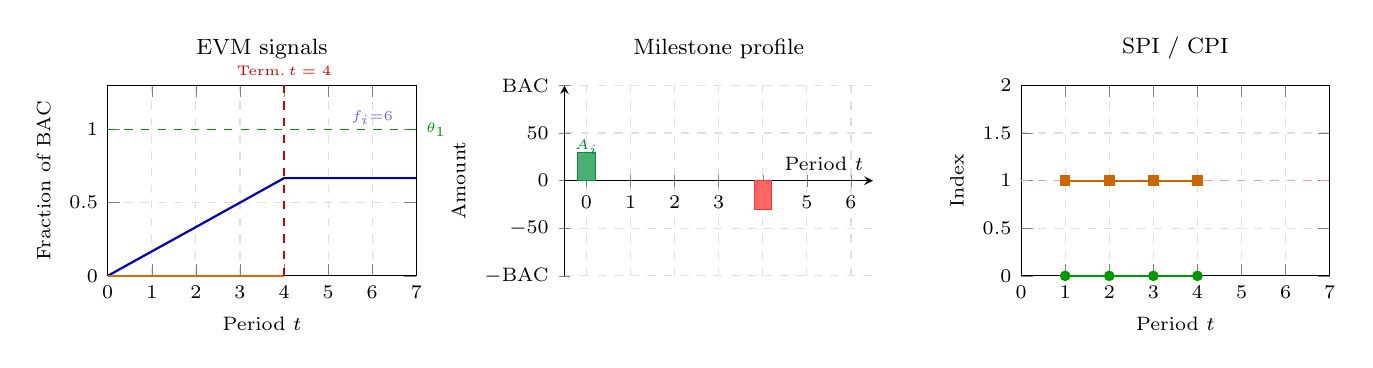
\begin{tikzpicture}[font=\footnotesize]
\begin{scope}
\begin{axis}[
    name=evmsp2c_p1,
    width=5.5cm, height=4.0cm,
    title={\footnotesize EVM signals},
    xlabel={Period $t$}, ylabel={Fraction of $\BAC$},
    xmin=0, xmax=7, ymin=0, ymax=1.30,
    xtick={0,1,2,3,4,5,6,7},
    ytick={0,0.5,1},
    grid=major, grid style={dashed,gray!25},
    tick label style={font=\scriptsize},
    label style={font=\scriptsize}, title style={font=\scriptsize},
    clip=false,
  ]
  \addplot[thick,blue!70!black] coordinates {(0,0) (1,0.167) (2,0.333) (3,0.5) (4,0.667) (7,0.667)};
  \addplot[thick,green!55!black] coordinates {(0,0) (1,0) (2,0) (3,0) (4,0)};
  \addplot[thick,orange!85!black] coordinates {(0,0) (1,0) (2,0) (3,0) (4,0)};
  \draw[green!60!black,dashed,thin] (axis cs:0,1)--(axis cs:7,1) node[right,green!60!black,font=\tiny] {$\theta_{1}$};
  \node[font=\tiny,blue!60] at (axis cs:6,1.08) {$f_i{=}6$};
  \draw[red!80!black,dashed,thick] (axis cs:4,0)--(axis cs:4,1.30) node[above,font=\tiny,red!80!black] {Term.\,$t=4$};
\end{axis}
\end{scope}

\begin{scope}[xshift=5.8cm]
\begin{axis}[
    name=mssp2c_p1,
    width=5.5cm, height=4.0cm,
    title={\footnotesize Milestone profile},
    xlabel={Period $t$}, ylabel={Amount},
    xmin=-0.5, xmax=6.5, ymin=-100, ymax=100,
    xtick={0,1,2,3,4,5,6},
    ytick={-100,-50,0,50,100},
    yticklabels={$-\BAC$,$-50$,$0$,$50$,$\BAC$},
    grid=major, grid style={dashed,gray!25},
    tick label style={font=\scriptsize},
    label style={font=\scriptsize}, title style={font=\scriptsize},
    axis x line=center, axis y line=left,
    clip=false,
  ]
  \addplot[ybar,bar width=0.22cm,fill=red!60,draw=red!80] coordinates {(4,-30)};
  \addplot[ybar,bar width=0.22cm,fill=msgreen!70,draw=msgreen] coordinates {(0,30)};
  \node[font=\tiny,msgreen] at (axis cs:0,35) {$A_i$};
\end{axis}
\end{scope}

\begin{scope}[xshift=11.6cm]
\begin{axis}[
    name=spicpisp2c_p1,
    width=5.5cm, height=4.0cm,
    title={\footnotesize SPI / CPI},
    xlabel={Period $t$}, ylabel={Index},
    xmin=0, xmax=7, ymin=0, ymax=2,
    xtick={0,1,2,3,4,5,6,7},
    ytick={0,0.5,1,1.5,2},
    grid=major, grid style={dashed,gray!25},
    tick label style={font=\scriptsize},
    label style={font=\scriptsize}, title style={font=\scriptsize},
    clip=false,
  ]
  \draw[red!40,dashed,thin] (axis cs:0,1)--(axis cs:7,1);
  \addplot[thick,green!60!black,mark=*,mark size=1.5pt] coordinates {(1,0) (2,0) (3,0) (4,0)};
  \addplot[thick,orange!80!black,mark=square*,mark size=1.5pt] coordinates {(1,1) (2,1) (3,1) (4,1)};
\end{axis}
\end{scope}

\end{tikzpicture}

\caption{SP-2c project view (single-project). Outcome: \texttt{terminated}. $Z^*=4.279$.}
\label{fig:sp2c_project}
\end{figure}

\begin{figure}[htbp]
\centering
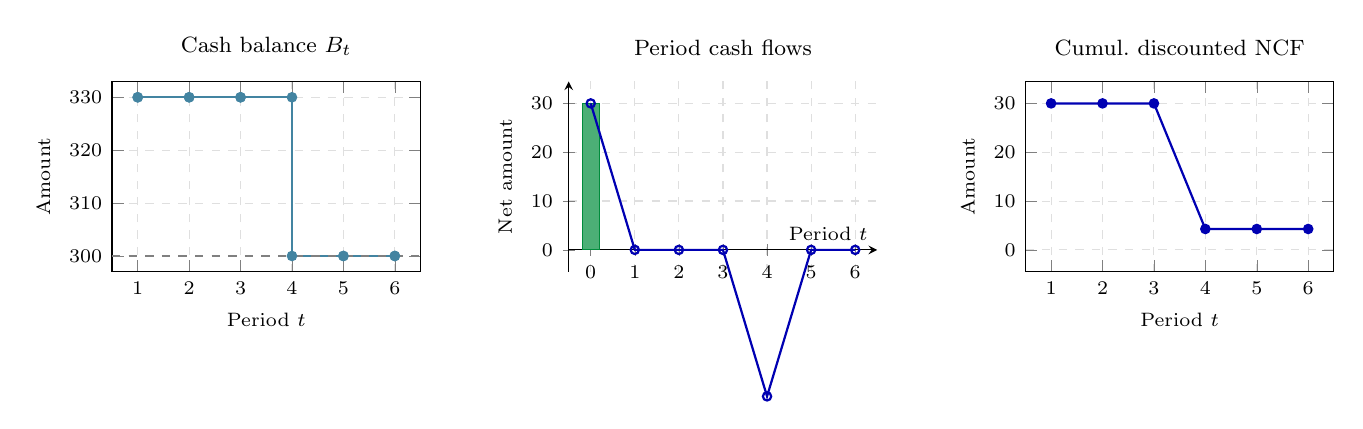
\begin{tikzpicture}[font=\footnotesize]
\begin{scope}
\begin{axis}[
    width=5.5cm, height=4.0cm,
    title={\footnotesize Cash balance $B_t$},
    xlabel={Period $t$}, ylabel={Amount},
    xmin=0.5, xmax=6.5,
    ymin=297, ymax=333,
    xtick={1,2,3,4,5,6},
    ytick={300,310,320,330},
    grid=major, grid style={dashed,gray!25},
    tick label style={font=\scriptsize},
    label style={font=\scriptsize}, title style={font=\scriptsize},
  ]
  \addplot[thick,cyan!60!black,mark=*,mark size=1.5pt] coordinates {(1,330) (1,330) (2,330) (2,330) (3,330) (3,330) (4,330) (4,300) (5,300) (5,300) (6,300) (6,300)};
  \draw[dashed,gray] (axis cs:0.5,300)--(axis cs:6.5,300) node[right,font=\tiny,gray] {$B_1$};
\end{axis}
\end{scope}

\begin{scope}[xshift=5.8cm]
\begin{axis}[
    width=5.5cm, height=4.0cm,
    title={\footnotesize Period cash flows},
    xlabel={Period $t$}, ylabel={Net amount},
    xmin=-0.5, xmax=6.5,
    ymin=-4.5, ymax=34.5,
    xtick={0,1,2,3,4,5,6},
    ytick={0,10,20,30},
    grid=major, grid style={dashed,gray!25},
    tick label style={font=\scriptsize},
    label style={font=\scriptsize}, title style={font=\scriptsize},
    axis x line=center, axis y line=left,
    clip=false,
  ]
  \addplot[ybar,bar width=0.22cm,fill=msgreen!70,draw=msgreen] coordinates {(0,30)};
  \addplot[thick,blue!70!black,mark=o,mark size=1.5pt] coordinates {(0,30) (1,0) (2,0) (3,0) (4,-30) (5,0) (6,0)};
\end{axis}
\end{scope}

\begin{scope}[xshift=11.6cm]
\begin{axis}[
    width=5.5cm, height=4.0cm,
    title={\footnotesize Cumul.\ discounted NCF},
    xlabel={Period $t$}, ylabel={Amount},
    xmin=0.5, xmax=6.5,
    ymin=-4.5, ymax=34.5,
    xtick={1,2,3,4,5,6},
    ytick={0,10,20,30},
    grid=major, grid style={dashed,gray!25},
    tick label style={font=\scriptsize},
    label style={font=\scriptsize}, title style={font=\scriptsize},
  ]
  \addplot[thick,blue!70!black,mark=*,mark size=1.5pt] coordinates {(1,30) (2,30) (3,30) (4,4.279) (5,4.279) (6,4.279)};
\end{axis}
\end{scope}

\end{tikzpicture}
\caption{SP-2c portfolio view. $Z^*=4.279$.}
\label{fig:sp2c_portfolio}
\end{figure}

\newpage

\subsection*{SP-2d  (Group~G3)}
\begin{center}
\begin{tabular}{ll}
\toprule
$n$,\;$H$ & $1$,\;$6$ \\
$\BAC,\;CP$ & $100,\;120$ \\
$s_i,\;f_i,\;D^{\mathrm{plan}}$ & $1,\;6,\;6$ \\
$\bar\eta$ & $1$ \\
$\alpha,\;A$ & $0.3,\;30$ \\
$M,\;\theta$ & $1,\;(1)$ \\
$\phi,\;e_{i,j}$ & $(1),\;(4)$ \\
$\mu,\;\Omega,\;\tau^{\mathrm{tol}}$ & $0.3,\;1,\;4$ \\
$B_1,\;\gamma$ & $300,\;0.95$ \\
$Z^*$ & $21.855$ \\
Outcome & \texttt{completed} \\
\bottomrule
\end{tabular}
\end{center}

\begin{center}
\begin{tabular}{rrrrrrrrrrl}
\toprule
$t$ & $x$ & $P$ & BCWS & BCWP & ACWP & SPI & CPI & $\tau$ & MS & $R_{\mathrm{net}}$\\
\midrule
1 & 0 & 0 & 0.167 & 0 & 0 & 0 & 1 & 4 & \texttt{---} & 0 \\
2 & 0 & 0 & 0.333 & 0 & 0 & 0 & 1 & 4 & \texttt{---} & 0 \\
3 & 0 & 0 & 0.5 & 0 & 0 & 0 & 1 & 4 & \texttt{---} & 0 \\
4 & 100 & 1 & 0.667 & 1 & 1 & 1.5 & 1 & 4 & \texttt{1} & 90 \\
5 & 0 & 1 & 0.833 & 1 & 1 & 1.2 & 1 & 4 & \texttt{---} & 0 \\
6 & 0 & 1 & 1 & 1 & 1 & 1 & 1 & 4 & \texttt{---} & 0 \\
\bottomrule
\end{tabular}
\end{center}
\paragraph{Portfolio strip.}
\begin{center}
\begin{tabular}{rrrrrrr}
\toprule
$t$ & $B_t$ & $\Sigma\mathrm{In}$ & $\Sigma\mathrm{Out}$ & $\Sigma\mathrm{Net}$ & $\gamma^{t-1}\mathrm{Net}$ & $Z_t^{\mathrm{cum}}$\\
\midrule
1 & 330 & 0 & 0 & 0 & 0 & 30 \\
2 & 330 & 0 & 0 & 0 & 0 & 30 \\
3 & 330 & 0 & 0 & 0 & 0 & 30 \\
4 & 320 & 90 & 100 & -10 & -8.574 & 21.426 \\
5 & 320 & 0 & 0 & 0 & 0 & 21.426 \\
6 & 320 & 0 & 0 & 0 & 0 & 21.426 \\
\bottomrule
\end{tabular}
\end{center}

\begin{figure}[htbp]
\centering
% === Project 1 row for SP-2d ===
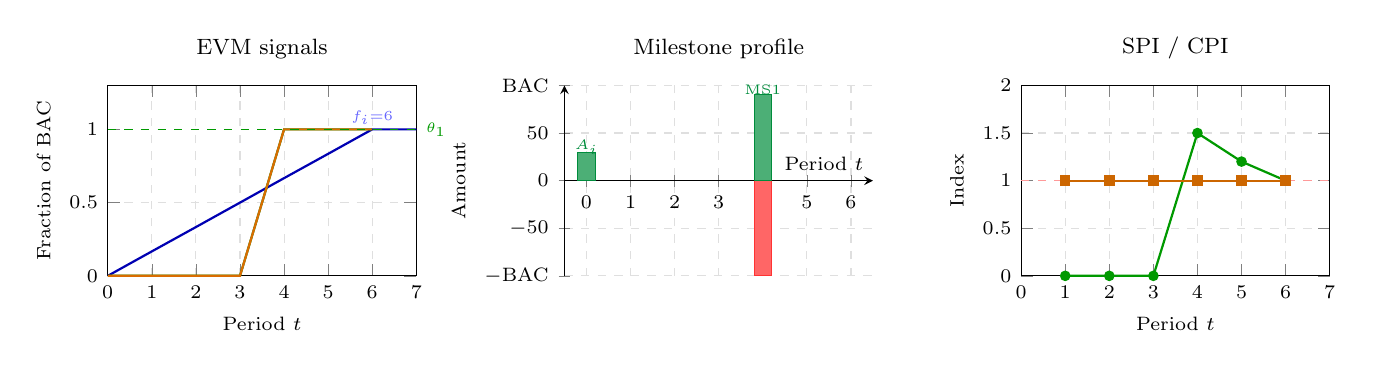
\begin{tikzpicture}[font=\footnotesize]
\begin{scope}
\begin{axis}[
    name=evmsp2d_p1,
    width=5.5cm, height=4.0cm,
    title={\footnotesize EVM signals},
    xlabel={Period $t$}, ylabel={Fraction of $\BAC$},
    xmin=0, xmax=7, ymin=0, ymax=1.30,
    xtick={0,1,2,3,4,5,6,7},
    ytick={0,0.5,1},
    grid=major, grid style={dashed,gray!25},
    tick label style={font=\scriptsize},
    label style={font=\scriptsize}, title style={font=\scriptsize},
    clip=false,
  ]
  \addplot[thick,blue!70!black] coordinates {(0,0) (1,0.167) (2,0.333) (3,0.5) (4,0.667) (5,0.833) (6,1) (7,1)};
  \addplot[thick,green!55!black] coordinates {(0,0) (1,0) (2,0) (3,0) (4,1) (5,1) (6,1)};
  \addplot[thick,orange!85!black] coordinates {(0,0) (1,0) (2,0) (3,0) (4,1) (5,1) (6,1)};
  \draw[green!60!black,dashed,thin] (axis cs:0,1)--(axis cs:7,1) node[right,green!60!black,font=\tiny] {$\theta_{1}$};
  \node[font=\tiny,blue!60] at (axis cs:6,1.08) {$f_i{=}6$};
\end{axis}
\end{scope}

\begin{scope}[xshift=5.8cm]
\begin{axis}[
    name=mssp2d_p1,
    width=5.5cm, height=4.0cm,
    title={\footnotesize Milestone profile},
    xlabel={Period $t$}, ylabel={Amount},
    xmin=-0.5, xmax=6.5, ymin=-100, ymax=100,
    xtick={0,1,2,3,4,5,6},
    ytick={-100,-50,0,50,100},
    yticklabels={$-\BAC$,$-50$,$0$,$50$,$\BAC$},
    grid=major, grid style={dashed,gray!25},
    tick label style={font=\scriptsize},
    label style={font=\scriptsize}, title style={font=\scriptsize},
    axis x line=center, axis y line=left,
    clip=false,
  ]
  \addplot[ybar,bar width=0.22cm,fill=red!60,draw=red!80] coordinates {(4,-100)};
  \addplot[ybar,bar width=0.22cm,fill=msgreen!70,draw=msgreen] coordinates {(0,30) (4,90)};
  \node[font=\tiny,msgreen] at (axis cs:4,95) {MS1};
  \node[font=\tiny,msgreen] at (axis cs:0,35) {$A_i$};
\end{axis}
\end{scope}

\begin{scope}[xshift=11.6cm]
\begin{axis}[
    name=spicpisp2d_p1,
    width=5.5cm, height=4.0cm,
    title={\footnotesize SPI / CPI},
    xlabel={Period $t$}, ylabel={Index},
    xmin=0, xmax=7, ymin=0, ymax=2,
    xtick={0,1,2,3,4,5,6,7},
    ytick={0,0.5,1,1.5,2},
    grid=major, grid style={dashed,gray!25},
    tick label style={font=\scriptsize},
    label style={font=\scriptsize}, title style={font=\scriptsize},
    clip=false,
  ]
  \draw[red!40,dashed,thin] (axis cs:0,1)--(axis cs:7,1);
  \addplot[thick,green!60!black,mark=*,mark size=1.5pt] coordinates {(1,0) (2,0) (3,0) (4,1.5) (5,1.2) (6,1)};
  \addplot[thick,orange!80!black,mark=square*,mark size=1.5pt] coordinates {(1,1) (2,1) (3,1) (4,1) (5,1) (6,1)};
\end{axis}
\end{scope}

\end{tikzpicture}

\caption{SP-2d project view (single-project). Outcome: \texttt{completed}. $Z^*=21.855$.}
\label{fig:sp2d_project}
\end{figure}

\begin{figure}[htbp]
\centering
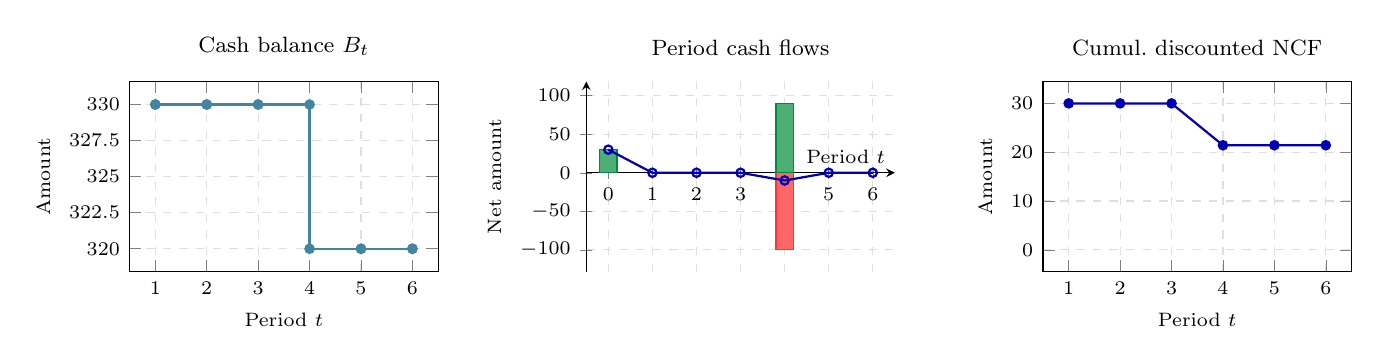
\begin{tikzpicture}[font=\footnotesize]
\begin{scope}
\begin{axis}[
    width=5.5cm, height=4.0cm,
    title={\footnotesize Cash balance $B_t$},
    xlabel={Period $t$}, ylabel={Amount},
    xmin=0.5, xmax=6.5,
    ymin=318.4, ymax=331.6,
    xtick={1,2,3,4,5,6},
    ytick={320,322.5,325,327.5,330},
    grid=major, grid style={dashed,gray!25},
    tick label style={font=\scriptsize},
    label style={font=\scriptsize}, title style={font=\scriptsize},
  ]
  \addplot[thick,cyan!60!black,mark=*,mark size=1.5pt] coordinates {(1,330) (1,330) (2,330) (2,330) (3,330) (3,330) (4,330) (4,320) (5,320) (5,320) (6,320) (6,320)};
  \draw[dashed,gray] (axis cs:0.5,300)--(axis cs:6.5,300) node[right,font=\tiny,gray] {$B_1$};
\end{axis}
\end{scope}

\begin{scope}[xshift=5.8cm]
\begin{axis}[
    width=5.5cm, height=4.0cm,
    title={\footnotesize Period cash flows},
    xlabel={Period $t$}, ylabel={Net amount},
    xmin=-0.5, xmax=6.5,
    ymin=-128.5, ymax=118.5,
    xtick={0,1,2,3,4,5,6},
    ytick={-100,-50,0,50,100},
    grid=major, grid style={dashed,gray!25},
    tick label style={font=\scriptsize},
    label style={font=\scriptsize}, title style={font=\scriptsize},
    axis x line=center, axis y line=left,
    clip=false,
  ]
  \addplot[ybar,bar width=0.22cm,fill=red!60,draw=red!80] coordinates {(4,-100)};
  \addplot[ybar,bar width=0.22cm,fill=msgreen!70,draw=msgreen] coordinates {(0,30) (4,90)};
  \addplot[thick,blue!70!black,mark=o,mark size=1.5pt] coordinates {(0,30) (1,0) (2,0) (3,0) (4,-10) (5,0) (6,0)};
\end{axis}
\end{scope}

\begin{scope}[xshift=11.6cm]
\begin{axis}[
    width=5.5cm, height=4.0cm,
    title={\footnotesize Cumul.\ discounted NCF},
    xlabel={Period $t$}, ylabel={Amount},
    xmin=0.5, xmax=6.5,
    ymin=-4.5, ymax=34.5,
    xtick={1,2,3,4,5,6},
    ytick={0,10,20,30},
    grid=major, grid style={dashed,gray!25},
    tick label style={font=\scriptsize},
    label style={font=\scriptsize}, title style={font=\scriptsize},
  ]
  \addplot[thick,blue!70!black,mark=*,mark size=1.5pt] coordinates {(1,30) (2,30) (3,30) (4,21.426) (5,21.426) (6,21.426)};
\end{axis}
\end{scope}

\end{tikzpicture}
\caption{SP-2d portfolio view. $Z^*=21.855$.}
\label{fig:sp2d_portfolio}
\end{figure}

\newpage

\subsection*{SP-A  (Group~G3)}
\begin{center}
\begin{tabular}{ll}
\toprule
$n$,\;$H$ & $1$,\;$6$ \\
$\BAC,\;CP$ & $120,\;180$ \\
$s_i,\;f_i,\;D^{\mathrm{plan}}$ & $1,\;6,\;6$ \\
$\bar\eta$ & $1$ \\
$\alpha,\;A$ & $0.2,\;36$ \\
$M,\;\theta$ & $3,\;(0.333,0.667,1)$ \\
$\phi,\;e_{i,j}$ & $(0.333,0.333,0.333),\;(1,3,5)$ \\
$\mu,\;\Omega,\;\tau^{\mathrm{tol}}$ & $0.5,\;2,\;2$ \\
$B_1,\;\gamma$ & $300,\;0.95$ \\
$Z^*$ & $59.43$ \\
Outcome & \texttt{completed} \\
\bottomrule
\end{tabular}
\end{center}

\begin{center}
\begin{tabular}{rrrrrrrrrrl}
\toprule
$t$ & $x$ & $P$ & BCWS & BCWP & ACWP & SPI & CPI & $\tau$ & MS & $R_{\mathrm{net}}$\\
\midrule
1 & 40 & 0.333 & 0.167 & 0.333 & 0.333 & 2 & 1 & 2 & \texttt{1} & 60 \\
2 & 0 & 0.333 & 0.333 & 0.333 & 0.333 & 1 & 1 & 2 & \texttt{---} & 0 \\
3 & 40 & 0.667 & 0.5 & 0.667 & 0.667 & 1.333 & 1 & 2 & \texttt{2} & 42 \\
4 & 0 & 0.667 & 0.667 & 0.667 & 0.667 & 1 & 1 & 2 & \texttt{---} & 0 \\
5 & 40 & 1 & 0.833 & 1 & 1 & 1.2 & 1 & 2 & \texttt{3} & 42 \\
6 & 0 & 1 & 1 & 1 & 1 & 1 & 1 & 2 & \texttt{---} & 0 \\
\bottomrule
\end{tabular}
\end{center}
\paragraph{Portfolio strip.}
\begin{center}
\begin{tabular}{rrrrrrr}
\toprule
$t$ & $B_t$ & $\Sigma\mathrm{In}$ & $\Sigma\mathrm{Out}$ & $\Sigma\mathrm{Net}$ & $\gamma^{t-1}\mathrm{Net}$ & $Z_t^{\mathrm{cum}}$\\
\midrule
1 & 356 & 60 & 40 & 20 & 20 & 56 \\
2 & 356 & 0 & 0 & 0 & 0 & 56 \\
3 & 358 & 42 & 40 & 2 & 1.805 & 57.805 \\
4 & 358 & 0 & 0 & 0 & 0 & 57.805 \\
5 & 360 & 42 & 40 & 2 & 1.629 & 59.434 \\
6 & 360 & 0 & 0 & 0 & 0 & 59.434 \\
\bottomrule
\end{tabular}
\end{center}

\begin{figure}[htbp]
\centering
% === Project 1 row for SP-A ===
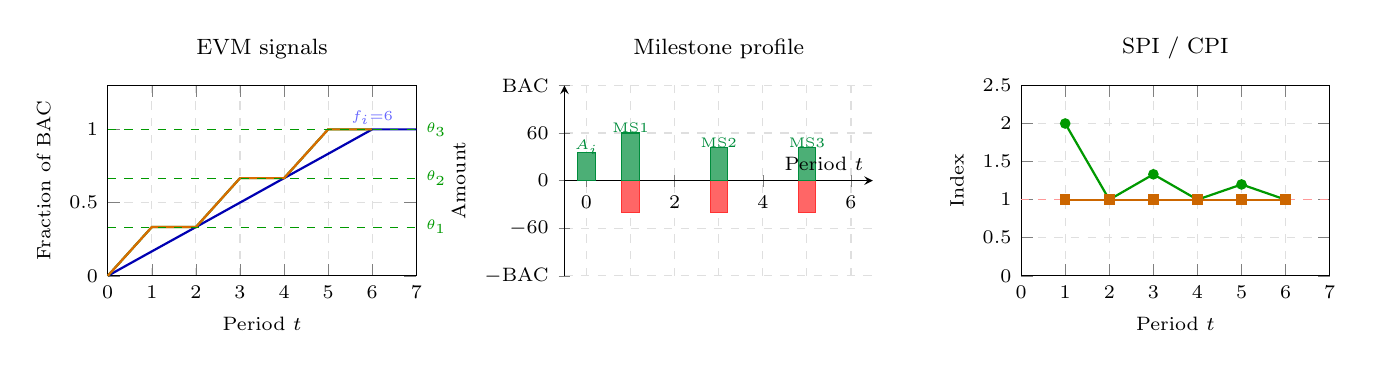
\begin{tikzpicture}[font=\footnotesize]
\begin{scope}
\begin{axis}[
    name=evmspa_p1,
    width=5.5cm, height=4.0cm,
    title={\footnotesize EVM signals},
    xlabel={Period $t$}, ylabel={Fraction of $\BAC$},
    xmin=0, xmax=7, ymin=0, ymax=1.30,
    xtick={0,1,2,3,4,5,6,7},
    ytick={0,0.5,1},
    grid=major, grid style={dashed,gray!25},
    tick label style={font=\scriptsize},
    label style={font=\scriptsize}, title style={font=\scriptsize},
    clip=false,
  ]
  \addplot[thick,blue!70!black] coordinates {(0,0) (1,0.167) (2,0.333) (3,0.5) (4,0.667) (5,0.833) (6,1) (7,1)};
  \addplot[thick,green!55!black] coordinates {(0,0) (1,0.333) (2,0.333) (3,0.667) (4,0.667) (5,1) (6,1)};
  \addplot[thick,orange!85!black] coordinates {(0,0) (1,0.333) (2,0.333) (3,0.667) (4,0.667) (5,1) (6,1)};
  \draw[green!60!black,dashed,thin] (axis cs:0,0.333)--(axis cs:7,0.333) node[right,green!60!black,font=\tiny] {$\theta_{1}$};
  \draw[green!60!black,dashed,thin] (axis cs:0,0.667)--(axis cs:7,0.667) node[right,green!60!black,font=\tiny] {$\theta_{2}$};
  \draw[green!60!black,dashed,thin] (axis cs:0,1)--(axis cs:7,1) node[right,green!60!black,font=\tiny] {$\theta_{3}$};
  \node[font=\tiny,blue!60] at (axis cs:6,1.08) {$f_i{=}6$};
\end{axis}
\end{scope}

\begin{scope}[xshift=5.8cm]
\begin{axis}[
    name=msspa_p1,
    width=5.5cm, height=4.0cm,
    title={\footnotesize Milestone profile},
    xlabel={Period $t$}, ylabel={Amount},
    xmin=-0.5, xmax=6.5, ymin=-120, ymax=120,
    xtick={0,1,2,3,4,5,6},
    ytick={-120,-60,0,60,120},
    yticklabels={$-\BAC$,$-60$,$0$,$60$,$\BAC$},
    grid=major, grid style={dashed,gray!25},
    tick label style={font=\scriptsize},
    label style={font=\scriptsize}, title style={font=\scriptsize},
    axis x line=center, axis y line=left,
    clip=false,
  ]
  \addplot[ybar,bar width=0.22cm,fill=red!60,draw=red!80] coordinates {(1,-40) (3,-40) (5,-40)};
  \addplot[ybar,bar width=0.22cm,fill=msgreen!70,draw=msgreen] coordinates {(0,36) (1,60) (3,42) (5,42)};
  \node[font=\tiny,msgreen] at (axis cs:1,66) {MS1};
  \node[font=\tiny,msgreen] at (axis cs:3,48) {MS2};
  \node[font=\tiny,msgreen] at (axis cs:5,48) {MS3};
  \node[font=\tiny,msgreen] at (axis cs:0,42) {$A_i$};
\end{axis}
\end{scope}

\begin{scope}[xshift=11.6cm]
\begin{axis}[
    name=spicpispa_p1,
    width=5.5cm, height=4.0cm,
    title={\footnotesize SPI / CPI},
    xlabel={Period $t$}, ylabel={Index},
    xmin=0, xmax=7, ymin=0, ymax=2.5,
    xtick={0,1,2,3,4,5,6,7},
    ytick={0,0.5,1,1.5,2,2.5},
    grid=major, grid style={dashed,gray!25},
    tick label style={font=\scriptsize},
    label style={font=\scriptsize}, title style={font=\scriptsize},
    clip=false,
  ]
  \draw[red!40,dashed,thin] (axis cs:0,1)--(axis cs:7,1);
  \addplot[thick,green!60!black,mark=*,mark size=1.5pt] coordinates {(1,2) (2,1) (3,1.333) (4,1) (5,1.2) (6,1)};
  \addplot[thick,orange!80!black,mark=square*,mark size=1.5pt] coordinates {(1,1) (2,1) (3,1) (4,1) (5,1) (6,1)};
\end{axis}
\end{scope}

\end{tikzpicture}

\caption{SP-A project view (single-project). Outcome: \texttt{completed}. $Z^*=59.43$.}
\label{fig:spa_project}
\end{figure}

\begin{figure}[htbp]
\centering
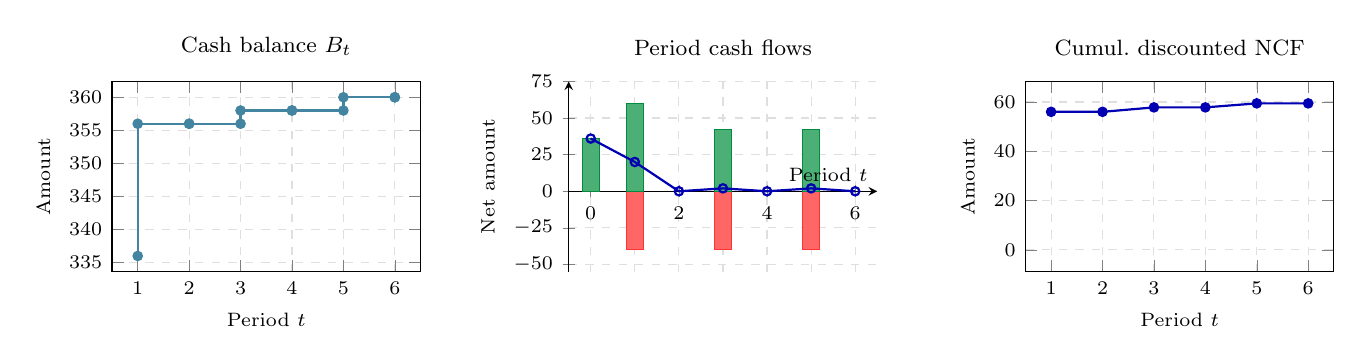
\begin{tikzpicture}[font=\footnotesize]
\begin{scope}
\begin{axis}[
    width=5.5cm, height=4.0cm,
    title={\footnotesize Cash balance $B_t$},
    xlabel={Period $t$}, ylabel={Amount},
    xmin=0.5, xmax=6.5,
    ymin=333.6, ymax=362.4,
    xtick={1,2,3,4,5,6},
    ytick={335,340,345,350,355,360},
    grid=major, grid style={dashed,gray!25},
    tick label style={font=\scriptsize},
    label style={font=\scriptsize}, title style={font=\scriptsize},
  ]
  \addplot[thick,cyan!60!black,mark=*,mark size=1.5pt] coordinates {(1,336) (1,356) (2,356) (2,356) (3,356) (3,358) (4,358) (4,358) (5,358) (5,360) (6,360) (6,360)};
  \draw[dashed,gray] (axis cs:0.5,300)--(axis cs:6.5,300) node[right,font=\tiny,gray] {$B_1$};
\end{axis}
\end{scope}

\begin{scope}[xshift=5.8cm]
\begin{axis}[
    width=5.5cm, height=4.0cm,
    title={\footnotesize Period cash flows},
    xlabel={Period $t$}, ylabel={Net amount},
    xmin=-0.5, xmax=6.5,
    ymin=-55, ymax=75,
    xtick={0,1,2,3,4,5,6},
    ytick={-50,-25,0,25,50,75},
    grid=major, grid style={dashed,gray!25},
    tick label style={font=\scriptsize},
    label style={font=\scriptsize}, title style={font=\scriptsize},
    axis x line=center, axis y line=left,
    clip=false,
  ]
  \addplot[ybar,bar width=0.22cm,fill=red!60,draw=red!80] coordinates {(1,-40) (3,-40) (5,-40)};
  \addplot[ybar,bar width=0.22cm,fill=msgreen!70,draw=msgreen] coordinates {(0,36) (1,60) (3,42) (5,42)};
  \addplot[thick,blue!70!black,mark=o,mark size=1.5pt] coordinates {(0,36) (1,20) (2,0) (3,2) (4,0) (5,2) (6,0)};
\end{axis}
\end{scope}

\begin{scope}[xshift=11.6cm]
\begin{axis}[
    width=5.5cm, height=4.0cm,
    title={\footnotesize Cumul.\ discounted NCF},
    xlabel={Period $t$}, ylabel={Amount},
    xmin=0.5, xmax=6.5,
    ymin=-8.915, ymax=68.349,
    xtick={1,2,3,4,5,6},
    ytick={0,20,40,60},
    grid=major, grid style={dashed,gray!25},
    tick label style={font=\scriptsize},
    label style={font=\scriptsize}, title style={font=\scriptsize},
  ]
  \addplot[thick,blue!70!black,mark=*,mark size=1.5pt] coordinates {(1,56) (2,56) (3,57.805) (4,57.805) (5,59.434) (6,59.434)};
\end{axis}
\end{scope}

\end{tikzpicture}
\caption{SP-A portfolio view. $Z^*=59.43$.}
\label{fig:spa_portfolio}
\end{figure}

\newpage

\subsection*{SP-B  (Group~G3)}
\begin{center}
\begin{tabular}{ll}
\toprule
$n$,\;$H$ & $1$,\;$4$ \\
$\BAC,\;CP$ & $60,\;90$ \\
$s_i,\;f_i,\;D^{\mathrm{plan}}$ & $1,\;4,\;3$ \\
$\bar\eta$ & $1$ \\
$\alpha,\;A$ & $0.2,\;18$ \\
$M,\;\theta$ & $3,\;(0.333,0.667,1)$ \\
$\phi,\;e_{i,j}$ & $(0.333,0.333,0.333),\;(1,2,3)$ \\
$\mu,\;\Omega,\;\tau^{\mathrm{tol}}$ & $0.5,\;2,\;2$ \\
$B_1,\;\gamma$ & $300,\;0.95$ \\
$Z^*$ & $28.975$ \\
Outcome & \texttt{completed} \\
\bottomrule
\end{tabular}
\end{center}

\begin{center}
\begin{tabular}{rrrrrrrrrrl}
\toprule
$t$ & $x$ & $P$ & BCWS & BCWP & ACWP & SPI & CPI & $\tau$ & MS & $R_{\mathrm{net}}$\\
\midrule
1 & 20 & 0.333 & 0.333 & 0.333 & 0.333 & 1 & 1 & 2 & \texttt{1} & 21 \\
2 & 20 & 0.667 & 0.667 & 0.667 & 0.667 & 1 & 1 & 2 & \texttt{2} & 21 \\
3 & 20 & 1 & 1 & 1 & 1 & 1 & 1 & 2 & \texttt{3} & 30 \\
4 & 0 & 1 & 1 & 1 & 1 & 1 & 1 & 2 & \texttt{---} & 0 \\
\bottomrule
\end{tabular}
\end{center}
\paragraph{Portfolio strip.}
\begin{center}
\begin{tabular}{rrrrrrr}
\toprule
$t$ & $B_t$ & $\Sigma\mathrm{In}$ & $\Sigma\mathrm{Out}$ & $\Sigma\mathrm{Net}$ & $\gamma^{t-1}\mathrm{Net}$ & $Z_t^{\mathrm{cum}}$\\
\midrule
1 & 319 & 21 & 20 & 1 & 1 & 19 \\
2 & 320 & 21 & 20 & 1 & 0.95 & 19.95 \\
3 & 330 & 30 & 20 & 10 & 9.025 & 28.975 \\
4 & 330 & 0 & 0 & 0 & 0 & 28.975 \\
\bottomrule
\end{tabular}
\end{center}

\begin{figure}[htbp]
\centering
% === Project 1 row for SP-B ===
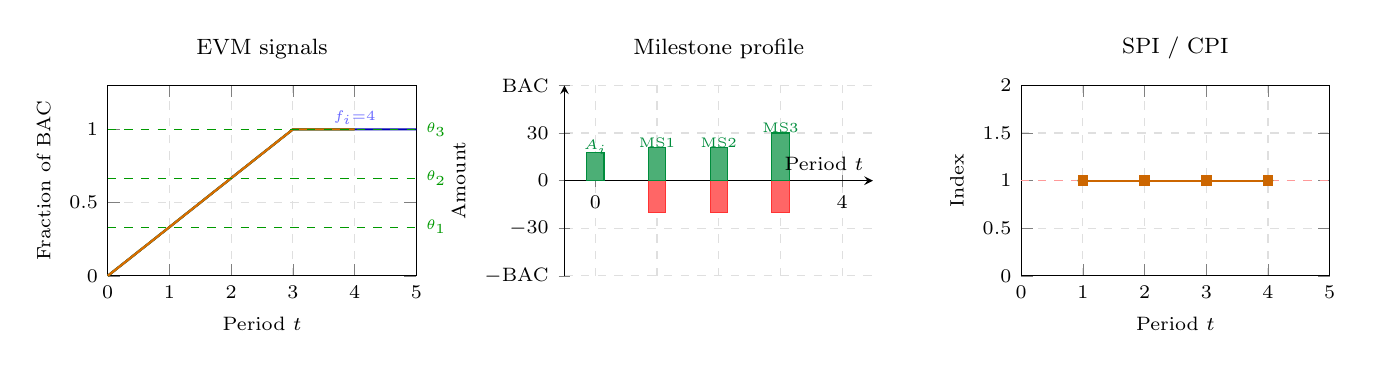
\begin{tikzpicture}[font=\footnotesize]
\begin{scope}
\begin{axis}[
    name=evmspb_p1,
    width=5.5cm, height=4.0cm,
    title={\footnotesize EVM signals},
    xlabel={Period $t$}, ylabel={Fraction of $\BAC$},
    xmin=0, xmax=5, ymin=0, ymax=1.30,
    xtick={0,1,2,3,4,5},
    ytick={0,0.5,1},
    grid=major, grid style={dashed,gray!25},
    tick label style={font=\scriptsize},
    label style={font=\scriptsize}, title style={font=\scriptsize},
    clip=false,
  ]
  \addplot[thick,blue!70!black] coordinates {(0,0) (1,0.333) (2,0.667) (3,1) (4,1) (5,1)};
  \addplot[thick,green!55!black] coordinates {(0,0) (1,0.333) (2,0.667) (3,1) (4,1)};
  \addplot[thick,orange!85!black] coordinates {(0,0) (1,0.333) (2,0.667) (3,1) (4,1)};
  \draw[green!60!black,dashed,thin] (axis cs:0,0.333)--(axis cs:5,0.333) node[right,green!60!black,font=\tiny] {$\theta_{1}$};
  \draw[green!60!black,dashed,thin] (axis cs:0,0.667)--(axis cs:5,0.667) node[right,green!60!black,font=\tiny] {$\theta_{2}$};
  \draw[green!60!black,dashed,thin] (axis cs:0,1)--(axis cs:5,1) node[right,green!60!black,font=\tiny] {$\theta_{3}$};
  \node[font=\tiny,blue!60] at (axis cs:4,1.08) {$f_i{=}4$};
\end{axis}
\end{scope}

\begin{scope}[xshift=5.8cm]
\begin{axis}[
    name=msspb_p1,
    width=5.5cm, height=4.0cm,
    title={\footnotesize Milestone profile},
    xlabel={Period $t$}, ylabel={Amount},
    xmin=-0.5, xmax=4.5, ymin=-60, ymax=60,
    xtick={0,1,2,3,4},
    ytick={-60,-30,0,30,60},
    yticklabels={$-\BAC$,$-30$,$0$,$30$,$\BAC$},
    grid=major, grid style={dashed,gray!25},
    tick label style={font=\scriptsize},
    label style={font=\scriptsize}, title style={font=\scriptsize},
    axis x line=center, axis y line=left,
    clip=false,
  ]
  \addplot[ybar,bar width=0.22cm,fill=red!60,draw=red!80] coordinates {(1,-20) (2,-20) (3,-20)};
  \addplot[ybar,bar width=0.22cm,fill=msgreen!70,draw=msgreen] coordinates {(0,18) (1,21) (2,21) (3,30)};
  \node[font=\tiny,msgreen] at (axis cs:1,24) {MS1};
  \node[font=\tiny,msgreen] at (axis cs:2,24) {MS2};
  \node[font=\tiny,msgreen] at (axis cs:3,33) {MS3};
  \node[font=\tiny,msgreen] at (axis cs:0,21) {$A_i$};
\end{axis}
\end{scope}

\begin{scope}[xshift=11.6cm]
\begin{axis}[
    name=spicpispb_p1,
    width=5.5cm, height=4.0cm,
    title={\footnotesize SPI / CPI},
    xlabel={Period $t$}, ylabel={Index},
    xmin=0, xmax=5, ymin=0, ymax=2,
    xtick={0,1,2,3,4,5},
    ytick={0,0.5,1,1.5,2},
    grid=major, grid style={dashed,gray!25},
    tick label style={font=\scriptsize},
    label style={font=\scriptsize}, title style={font=\scriptsize},
    clip=false,
  ]
  \draw[red!40,dashed,thin] (axis cs:0,1)--(axis cs:5,1);
  \addplot[thick,green!60!black,mark=*,mark size=1.5pt] coordinates {(1,1) (2,1) (3,1) (4,1)};
  \addplot[thick,orange!80!black,mark=square*,mark size=1.5pt] coordinates {(1,1) (2,1) (3,1) (4,1)};
\end{axis}
\end{scope}

\end{tikzpicture}

\caption{SP-B project view (single-project). Outcome: \texttt{completed}. $Z^*=28.975$.}
\label{fig:spb_project}
\end{figure}

\begin{figure}[htbp]
\centering
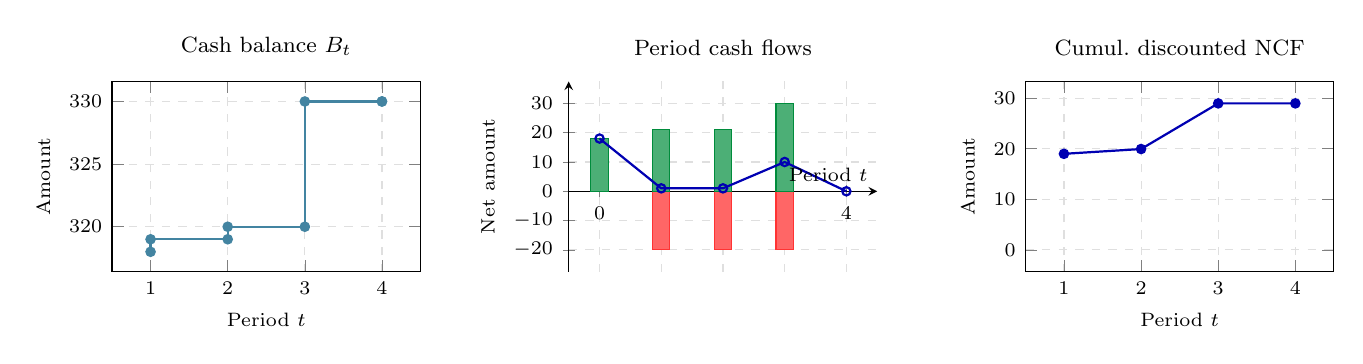
\begin{tikzpicture}[font=\footnotesize]
\begin{scope}
\begin{axis}[
    width=5.5cm, height=4.0cm,
    title={\footnotesize Cash balance $B_t$},
    xlabel={Period $t$}, ylabel={Amount},
    xmin=0.5, xmax=4.5,
    ymin=316.4, ymax=331.6,
    xtick={1,2,3,4},
    ytick={320,325,330},
    grid=major, grid style={dashed,gray!25},
    tick label style={font=\scriptsize},
    label style={font=\scriptsize}, title style={font=\scriptsize},
  ]
  \addplot[thick,cyan!60!black,mark=*,mark size=1.5pt] coordinates {(1,318) (1,319) (2,319) (2,320) (3,320) (3,330) (4,330) (4,330)};
  \draw[dashed,gray] (axis cs:0.5,300)--(axis cs:4.5,300) node[right,font=\tiny,gray] {$B_1$};
\end{axis}
\end{scope}

\begin{scope}[xshift=5.8cm]
\begin{axis}[
    width=5.5cm, height=4.0cm,
    title={\footnotesize Period cash flows},
    xlabel={Period $t$}, ylabel={Net amount},
    xmin=-0.5, xmax=4.5,
    ymin=-27.5, ymax=37.5,
    xtick={0,1,2,3,4},
    ytick={-20,-10,0,10,20,30},
    grid=major, grid style={dashed,gray!25},
    tick label style={font=\scriptsize},
    label style={font=\scriptsize}, title style={font=\scriptsize},
    axis x line=center, axis y line=left,
    clip=false,
  ]
  \addplot[ybar,bar width=0.22cm,fill=red!60,draw=red!80] coordinates {(1,-20) (2,-20) (3,-20)};
  \addplot[ybar,bar width=0.22cm,fill=msgreen!70,draw=msgreen] coordinates {(0,18) (1,21) (2,21) (3,30)};
  \addplot[thick,blue!70!black,mark=o,mark size=1.5pt] coordinates {(0,18) (1,1) (2,1) (3,10) (4,0)};
\end{axis}
\end{scope}

\begin{scope}[xshift=11.6cm]
\begin{axis}[
    width=5.5cm, height=4.0cm,
    title={\footnotesize Cumul.\ discounted NCF},
    xlabel={Period $t$}, ylabel={Amount},
    xmin=0.5, xmax=4.5,
    ymin=-4.346, ymax=33.321,
    xtick={1,2,3,4},
    ytick={0,10,20,30},
    grid=major, grid style={dashed,gray!25},
    tick label style={font=\scriptsize},
    label style={font=\scriptsize}, title style={font=\scriptsize},
  ]
  \addplot[thick,blue!70!black,mark=*,mark size=1.5pt] coordinates {(1,19) (2,19.95) (3,28.975) (4,28.975)};
\end{axis}
\end{scope}

\end{tikzpicture}
\caption{SP-B portfolio view. $Z^*=28.975$.}
\label{fig:spb_portfolio}
\end{figure}

\newpage


\subsection*{Group 4: Retention}

\subsection*{SP-C  (Group~G4)}
\begin{center}
\begin{tabular}{ll}
\toprule
$n$,\;$H$ & $1$,\;$6$ \\
$\BAC,\;CP$ & $60,\;90$ \\
$s_i,\;f_i,\;D^{\mathrm{plan}}$ & $1,\;6,\;6$ \\
$\bar\eta$ & $1$ \\
$\rho$ & $0.1$ \\
$M,\;\theta$ & $3,\;(0.333,0.667,1)$ \\
$\phi,\;e_{i,j}$ & $(0.333,0.333,0.333),\;(1,3,5)$ \\
$\mu,\;\Omega,\;\tau^{\mathrm{tol}}$ & $0.5,\;2,\;2$ \\
$B_1,\;\gamma$ & $300,\;0.95$ \\
$Z^*$ & $26.35$ \\
Outcome & \texttt{completed} \\
\bottomrule
\end{tabular}
\end{center}

\begin{center}
\begin{tabular}{rrrrrrrrrrl}
\toprule
$t$ & $x$ & $P$ & BCWS & BCWP & ACWP & SPI & CPI & $\tau$ & MS & $R_{\mathrm{net}}$\\
\midrule
1 & 20 & 0.333 & 0.167 & 0.333 & 0.333 & 2 & 1 & 2 & \texttt{1} & 27 \\
2 & 0 & 0.333 & 0.333 & 0.333 & 0.333 & 1 & 1 & 2 & \texttt{---} & 0 \\
3 & 20 & 0.667 & 0.5 & 0.667 & 0.667 & 1.333 & 1 & 2 & \texttt{2} & 27 \\
4 & 0 & 0.667 & 0.667 & 0.667 & 0.667 & 1 & 1 & 2 & \texttt{---} & 0 \\
5 & 20 & 1 & 0.833 & 1 & 1 & 1.2 & 1 & 2 & \texttt{3} & 36 \\
6 & 0 & 1 & 1 & 1 & 1 & 1 & 1 & 2 & \texttt{---} & 0 \\
\bottomrule
\end{tabular}
\end{center}
\paragraph{Portfolio strip.}
\begin{center}
\begin{tabular}{rrrrrrr}
\toprule
$t$ & $B_t$ & $\Sigma\mathrm{In}$ & $\Sigma\mathrm{Out}$ & $\Sigma\mathrm{Net}$ & $\gamma^{t-1}\mathrm{Net}$ & $Z_t^{\mathrm{cum}}$\\
\midrule
1 & 307 & 27 & 20 & 7 & 7 & 7 \\
2 & 307 & 0 & 0 & 0 & 0 & 7 \\
3 & 314 & 27 & 20 & 7 & 6.317 & 13.318 \\
4 & 314 & 0 & 0 & 0 & 0 & 13.318 \\
5 & 330 & 36 & 20 & 16 & 13.032 & 26.35 \\
6 & 330 & 0 & 0 & 0 & 0 & 26.35 \\
\bottomrule
\end{tabular}
\end{center}

\begin{figure}[htbp]
\centering
% === Project 1 row for SP-C ===
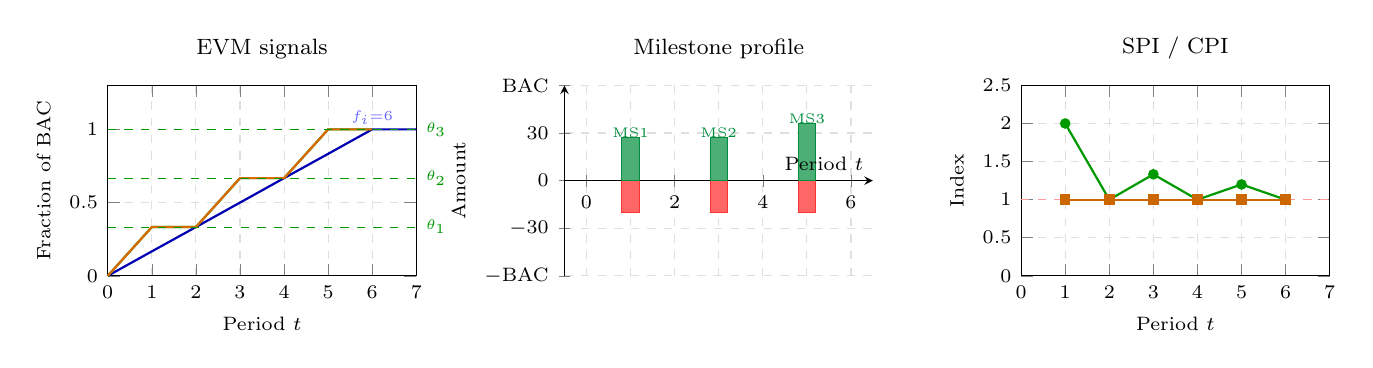
\begin{tikzpicture}[font=\footnotesize]
\begin{scope}
\begin{axis}[
    name=evmspc_p1,
    width=5.5cm, height=4.0cm,
    title={\footnotesize EVM signals},
    xlabel={Period $t$}, ylabel={Fraction of $\BAC$},
    xmin=0, xmax=7, ymin=0, ymax=1.30,
    xtick={0,1,2,3,4,5,6,7},
    ytick={0,0.5,1},
    grid=major, grid style={dashed,gray!25},
    tick label style={font=\scriptsize},
    label style={font=\scriptsize}, title style={font=\scriptsize},
    clip=false,
  ]
  \addplot[thick,blue!70!black] coordinates {(0,0) (1,0.167) (2,0.333) (3,0.5) (4,0.667) (5,0.833) (6,1) (7,1)};
  \addplot[thick,green!55!black] coordinates {(0,0) (1,0.333) (2,0.333) (3,0.667) (4,0.667) (5,1) (6,1)};
  \addplot[thick,orange!85!black] coordinates {(0,0) (1,0.333) (2,0.333) (3,0.667) (4,0.667) (5,1) (6,1)};
  \draw[green!60!black,dashed,thin] (axis cs:0,0.333)--(axis cs:7,0.333) node[right,green!60!black,font=\tiny] {$\theta_{1}$};
  \draw[green!60!black,dashed,thin] (axis cs:0,0.667)--(axis cs:7,0.667) node[right,green!60!black,font=\tiny] {$\theta_{2}$};
  \draw[green!60!black,dashed,thin] (axis cs:0,1)--(axis cs:7,1) node[right,green!60!black,font=\tiny] {$\theta_{3}$};
  \node[font=\tiny,blue!60] at (axis cs:6,1.08) {$f_i{=}6$};
\end{axis}
\end{scope}

\begin{scope}[xshift=5.8cm]
\begin{axis}[
    name=msspc_p1,
    width=5.5cm, height=4.0cm,
    title={\footnotesize Milestone profile},
    xlabel={Period $t$}, ylabel={Amount},
    xmin=-0.5, xmax=6.5, ymin=-60, ymax=60,
    xtick={0,1,2,3,4,5,6},
    ytick={-60,-30,0,30,60},
    yticklabels={$-\BAC$,$-30$,$0$,$30$,$\BAC$},
    grid=major, grid style={dashed,gray!25},
    tick label style={font=\scriptsize},
    label style={font=\scriptsize}, title style={font=\scriptsize},
    axis x line=center, axis y line=left,
    clip=false,
  ]
  \addplot[ybar,bar width=0.22cm,fill=red!60,draw=red!80] coordinates {(1,-20) (3,-20) (5,-20)};
  \addplot[ybar,bar width=0.22cm,fill=msgreen!70,draw=msgreen] coordinates {(1,27) (3,27) (5,36)};
  \node[font=\tiny,msgreen] at (axis cs:1,30) {MS1};
  \node[font=\tiny,msgreen] at (axis cs:3,30) {MS2};
  \node[font=\tiny,msgreen] at (axis cs:5,39) {MS3};
\end{axis}
\end{scope}

\begin{scope}[xshift=11.6cm]
\begin{axis}[
    name=spicpispc_p1,
    width=5.5cm, height=4.0cm,
    title={\footnotesize SPI / CPI},
    xlabel={Period $t$}, ylabel={Index},
    xmin=0, xmax=7, ymin=0, ymax=2.5,
    xtick={0,1,2,3,4,5,6,7},
    ytick={0,0.5,1,1.5,2,2.5},
    grid=major, grid style={dashed,gray!25},
    tick label style={font=\scriptsize},
    label style={font=\scriptsize}, title style={font=\scriptsize},
    clip=false,
  ]
  \draw[red!40,dashed,thin] (axis cs:0,1)--(axis cs:7,1);
  \addplot[thick,green!60!black,mark=*,mark size=1.5pt] coordinates {(1,2) (2,1) (3,1.333) (4,1) (5,1.2) (6,1)};
  \addplot[thick,orange!80!black,mark=square*,mark size=1.5pt] coordinates {(1,1) (2,1) (3,1) (4,1) (5,1) (6,1)};
\end{axis}
\end{scope}

\end{tikzpicture}

\caption{SP-C project view (single-project). Outcome: \texttt{completed}. $Z^*=26.35$.}
\label{fig:spc_project}
\end{figure}

\begin{figure}[htbp]
\centering
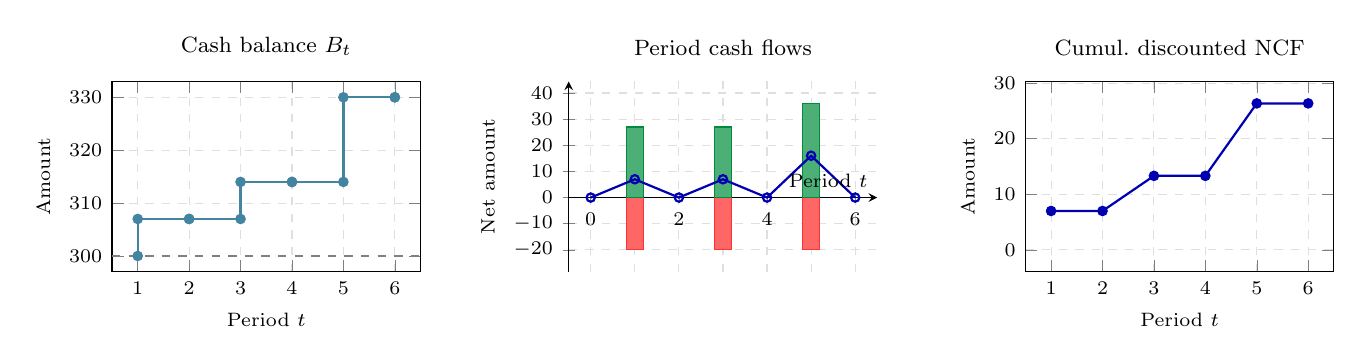
\begin{tikzpicture}[font=\footnotesize]
\begin{scope}
\begin{axis}[
    width=5.5cm, height=4.0cm,
    title={\footnotesize Cash balance $B_t$},
    xlabel={Period $t$}, ylabel={Amount},
    xmin=0.5, xmax=6.5,
    ymin=297, ymax=333,
    xtick={1,2,3,4,5,6},
    ytick={300,310,320,330},
    grid=major, grid style={dashed,gray!25},
    tick label style={font=\scriptsize},
    label style={font=\scriptsize}, title style={font=\scriptsize},
  ]
  \addplot[thick,cyan!60!black,mark=*,mark size=1.5pt] coordinates {(1,300) (1,307) (2,307) (2,307) (3,307) (3,314) (4,314) (4,314) (5,314) (5,330) (6,330) (6,330)};
  \draw[dashed,gray] (axis cs:0.5,300)--(axis cs:6.5,300) node[right,font=\tiny,gray] {$B_1$};
\end{axis}
\end{scope}

\begin{scope}[xshift=5.8cm]
\begin{axis}[
    width=5.5cm, height=4.0cm,
    title={\footnotesize Period cash flows},
    xlabel={Period $t$}, ylabel={Net amount},
    xmin=-0.5, xmax=6.5,
    ymin=-28.4, ymax=44.4,
    xtick={0,1,2,3,4,5,6},
    ytick={-20,-10,0,10,20,30,40},
    grid=major, grid style={dashed,gray!25},
    tick label style={font=\scriptsize},
    label style={font=\scriptsize}, title style={font=\scriptsize},
    axis x line=center, axis y line=left,
    clip=false,
  ]
  \addplot[ybar,bar width=0.22cm,fill=red!60,draw=red!80] coordinates {(1,-20) (3,-20) (5,-20)};
  \addplot[ybar,bar width=0.22cm,fill=msgreen!70,draw=msgreen] coordinates {(1,27) (3,27) (5,36)};
  \addplot[thick,blue!70!black,mark=o,mark size=1.5pt] coordinates {(0,0) (1,7) (2,0) (3,7) (4,0) (5,16) (6,0)};
\end{axis}
\end{scope}

\begin{scope}[xshift=11.6cm]
\begin{axis}[
    width=5.5cm, height=4.0cm,
    title={\footnotesize Cumul.\ discounted NCF},
    xlabel={Period $t$}, ylabel={Amount},
    xmin=0.5, xmax=6.5,
    ymin=-3.952, ymax=30.302,
    xtick={1,2,3,4,5,6},
    ytick={0,10,20,30},
    grid=major, grid style={dashed,gray!25},
    tick label style={font=\scriptsize},
    label style={font=\scriptsize}, title style={font=\scriptsize},
  ]
  \addplot[thick,blue!70!black,mark=*,mark size=1.5pt] coordinates {(1,7) (2,7) (3,13.318) (4,13.318) (5,26.35) (6,26.35)};
\end{axis}
\end{scope}

\end{tikzpicture}
\caption{SP-C portfolio view. $Z^*=26.35$.}
\label{fig:spc_portfolio}
\end{figure}

\newpage

\subsection*{SP-D  (Group~G4)}
\begin{center}
\begin{tabular}{ll}
\toprule
$n$,\;$H$ & $1$,\;$6$ \\
$\BAC,\;CP$ & $60,\;90$ \\
$s_i,\;f_i,\;D^{\mathrm{plan}}$ & $1,\;6,\;6$ \\
$\bar\eta$ & $1$ \\
$\alpha,\;A$ & $0.2,\;18$ \\
$\rho$ & $0.1$ \\
$M,\;\theta$ & $3,\;(0.333,0.667,1)$ \\
$\phi,\;e_{i,j}$ & $(0.333,0.333,0.333),\;(1,3,5)$ \\
$\mu,\;\Omega,\;\tau^{\mathrm{tol}}$ & $0.5,\;2,\;2$ \\
$B_1,\;\gamma$ & $300,\;0.95$ \\
$Z^*$ & $27.227$ \\
Outcome & \texttt{completed} \\
\bottomrule
\end{tabular}
\end{center}

\begin{center}
\begin{tabular}{rrrrrrrrrrl}
\toprule
$t$ & $x$ & $P$ & BCWS & BCWP & ACWP & SPI & CPI & $\tau$ & MS & $R_{\mathrm{net}}$\\
\midrule
1 & 20 & 0.333 & 0.167 & 0.333 & 0.333 & 2 & 1 & 2 & \texttt{1} & 18 \\
2 & 0 & 0.333 & 0.333 & 0.333 & 0.333 & 1 & 1 & 2 & \texttt{---} & 0 \\
3 & 20 & 0.667 & 0.5 & 0.667 & 0.667 & 1.333 & 1 & 2 & \texttt{2} & 18 \\
4 & 0 & 0.667 & 0.667 & 0.667 & 0.667 & 1 & 1 & 2 & \texttt{---} & 0 \\
5 & 20 & 1 & 0.833 & 1 & 1 & 1.2 & 1 & 2 & \texttt{3} & 36 \\
6 & 0 & 1 & 1 & 1 & 1 & 1 & 1 & 2 & \texttt{---} & 0 \\
\bottomrule
\end{tabular}
\end{center}
\paragraph{Portfolio strip.}
\begin{center}
\begin{tabular}{rrrrrrr}
\toprule
$t$ & $B_t$ & $\Sigma\mathrm{In}$ & $\Sigma\mathrm{Out}$ & $\Sigma\mathrm{Net}$ & $\gamma^{t-1}\mathrm{Net}$ & $Z_t^{\mathrm{cum}}$\\
\midrule
1 & 316 & 18 & 20 & -2 & -2 & 16 \\
2 & 316 & 0 & 0 & 0 & 0 & 16 \\
3 & 314 & 18 & 20 & -2 & -1.805 & 14.195 \\
4 & 314 & 0 & 0 & 0 & 0 & 14.195 \\
5 & 330 & 36 & 20 & 16 & 13.032 & 27.227 \\
6 & 330 & 0 & 0 & 0 & 0 & 27.227 \\
\bottomrule
\end{tabular}
\end{center}

\begin{figure}[htbp]
\centering
% === Project 1 row for SP-D ===
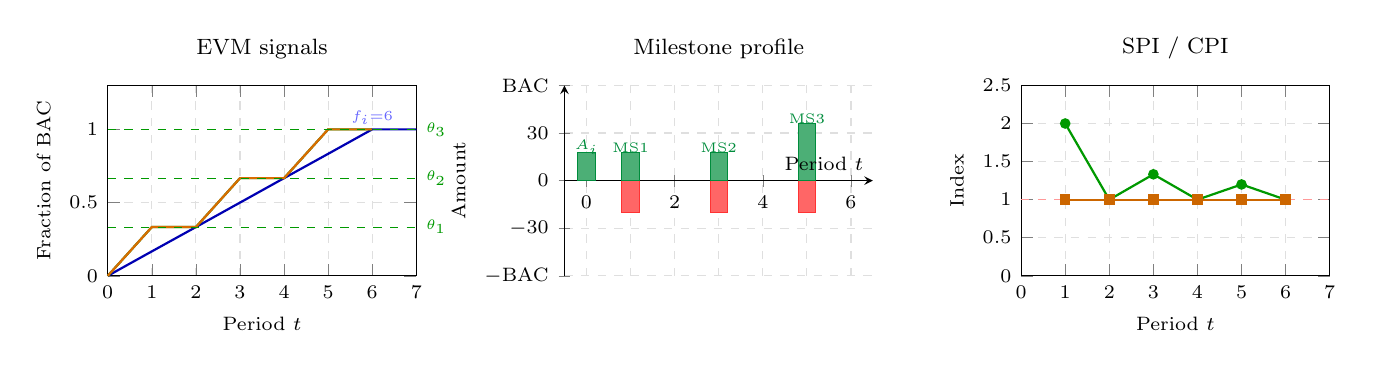
\begin{tikzpicture}[font=\footnotesize]
\begin{scope}
\begin{axis}[
    name=evmspd_p1,
    width=5.5cm, height=4.0cm,
    title={\footnotesize EVM signals},
    xlabel={Period $t$}, ylabel={Fraction of $\BAC$},
    xmin=0, xmax=7, ymin=0, ymax=1.30,
    xtick={0,1,2,3,4,5,6,7},
    ytick={0,0.5,1},
    grid=major, grid style={dashed,gray!25},
    tick label style={font=\scriptsize},
    label style={font=\scriptsize}, title style={font=\scriptsize},
    clip=false,
  ]
  \addplot[thick,blue!70!black] coordinates {(0,0) (1,0.167) (2,0.333) (3,0.5) (4,0.667) (5,0.833) (6,1) (7,1)};
  \addplot[thick,green!55!black] coordinates {(0,0) (1,0.333) (2,0.333) (3,0.667) (4,0.667) (5,1) (6,1)};
  \addplot[thick,orange!85!black] coordinates {(0,0) (1,0.333) (2,0.333) (3,0.667) (4,0.667) (5,1) (6,1)};
  \draw[green!60!black,dashed,thin] (axis cs:0,0.333)--(axis cs:7,0.333) node[right,green!60!black,font=\tiny] {$\theta_{1}$};
  \draw[green!60!black,dashed,thin] (axis cs:0,0.667)--(axis cs:7,0.667) node[right,green!60!black,font=\tiny] {$\theta_{2}$};
  \draw[green!60!black,dashed,thin] (axis cs:0,1)--(axis cs:7,1) node[right,green!60!black,font=\tiny] {$\theta_{3}$};
  \node[font=\tiny,blue!60] at (axis cs:6,1.08) {$f_i{=}6$};
\end{axis}
\end{scope}

\begin{scope}[xshift=5.8cm]
\begin{axis}[
    name=msspd_p1,
    width=5.5cm, height=4.0cm,
    title={\footnotesize Milestone profile},
    xlabel={Period $t$}, ylabel={Amount},
    xmin=-0.5, xmax=6.5, ymin=-60, ymax=60,
    xtick={0,1,2,3,4,5,6},
    ytick={-60,-30,0,30,60},
    yticklabels={$-\BAC$,$-30$,$0$,$30$,$\BAC$},
    grid=major, grid style={dashed,gray!25},
    tick label style={font=\scriptsize},
    label style={font=\scriptsize}, title style={font=\scriptsize},
    axis x line=center, axis y line=left,
    clip=false,
  ]
  \addplot[ybar,bar width=0.22cm,fill=red!60,draw=red!80] coordinates {(1,-20) (3,-20) (5,-20)};
  \addplot[ybar,bar width=0.22cm,fill=msgreen!70,draw=msgreen] coordinates {(0,18) (1,18) (3,18) (5,36)};
  \node[font=\tiny,msgreen] at (axis cs:1,21) {MS1};
  \node[font=\tiny,msgreen] at (axis cs:3,21) {MS2};
  \node[font=\tiny,msgreen] at (axis cs:5,39) {MS3};
  \node[font=\tiny,msgreen] at (axis cs:0,21) {$A_i$};
\end{axis}
\end{scope}

\begin{scope}[xshift=11.6cm]
\begin{axis}[
    name=spicpispd_p1,
    width=5.5cm, height=4.0cm,
    title={\footnotesize SPI / CPI},
    xlabel={Period $t$}, ylabel={Index},
    xmin=0, xmax=7, ymin=0, ymax=2.5,
    xtick={0,1,2,3,4,5,6,7},
    ytick={0,0.5,1,1.5,2,2.5},
    grid=major, grid style={dashed,gray!25},
    tick label style={font=\scriptsize},
    label style={font=\scriptsize}, title style={font=\scriptsize},
    clip=false,
  ]
  \draw[red!40,dashed,thin] (axis cs:0,1)--(axis cs:7,1);
  \addplot[thick,green!60!black,mark=*,mark size=1.5pt] coordinates {(1,2) (2,1) (3,1.333) (4,1) (5,1.2) (6,1)};
  \addplot[thick,orange!80!black,mark=square*,mark size=1.5pt] coordinates {(1,1) (2,1) (3,1) (4,1) (5,1) (6,1)};
\end{axis}
\end{scope}

\end{tikzpicture}

\caption{SP-D project view (single-project). Outcome: \texttt{completed}. $Z^*=27.227$.}
\label{fig:spd_project}
\end{figure}

\begin{figure}[htbp]
\centering
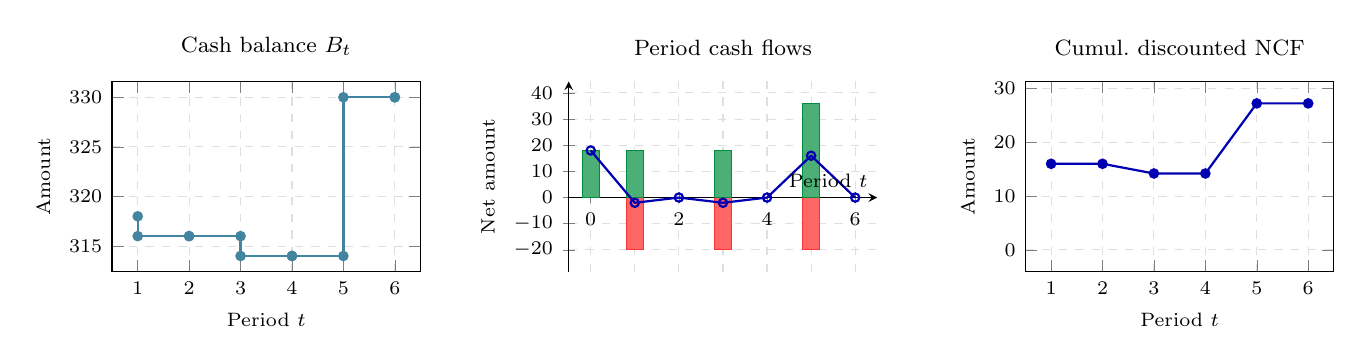
\begin{tikzpicture}[font=\footnotesize]
\begin{scope}
\begin{axis}[
    width=5.5cm, height=4.0cm,
    title={\footnotesize Cash balance $B_t$},
    xlabel={Period $t$}, ylabel={Amount},
    xmin=0.5, xmax=6.5,
    ymin=312.4, ymax=331.6,
    xtick={1,2,3,4,5,6},
    ytick={315,320,325,330},
    grid=major, grid style={dashed,gray!25},
    tick label style={font=\scriptsize},
    label style={font=\scriptsize}, title style={font=\scriptsize},
  ]
  \addplot[thick,cyan!60!black,mark=*,mark size=1.5pt] coordinates {(1,318) (1,316) (2,316) (2,316) (3,316) (3,314) (4,314) (4,314) (5,314) (5,330) (6,330) (6,330)};
  \draw[dashed,gray] (axis cs:0.5,300)--(axis cs:6.5,300) node[right,font=\tiny,gray] {$B_1$};
\end{axis}
\end{scope}

\begin{scope}[xshift=5.8cm]
\begin{axis}[
    width=5.5cm, height=4.0cm,
    title={\footnotesize Period cash flows},
    xlabel={Period $t$}, ylabel={Net amount},
    xmin=-0.5, xmax=6.5,
    ymin=-28.4, ymax=44.4,
    xtick={0,1,2,3,4,5,6},
    ytick={-20,-10,0,10,20,30,40},
    grid=major, grid style={dashed,gray!25},
    tick label style={font=\scriptsize},
    label style={font=\scriptsize}, title style={font=\scriptsize},
    axis x line=center, axis y line=left,
    clip=false,
  ]
  \addplot[ybar,bar width=0.22cm,fill=red!60,draw=red!80] coordinates {(1,-20) (3,-20) (5,-20)};
  \addplot[ybar,bar width=0.22cm,fill=msgreen!70,draw=msgreen] coordinates {(0,18) (1,18) (3,18) (5,36)};
  \addplot[thick,blue!70!black,mark=o,mark size=1.5pt] coordinates {(0,18) (1,-2) (2,0) (3,-2) (4,0) (5,16) (6,0)};
\end{axis}
\end{scope}

\begin{scope}[xshift=11.6cm]
\begin{axis}[
    width=5.5cm, height=4.0cm,
    title={\footnotesize Cumul.\ discounted NCF},
    xlabel={Period $t$}, ylabel={Amount},
    xmin=0.5, xmax=6.5,
    ymin=-4.084, ymax=31.311,
    xtick={1,2,3,4,5,6},
    ytick={0,10,20,30},
    grid=major, grid style={dashed,gray!25},
    tick label style={font=\scriptsize},
    label style={font=\scriptsize}, title style={font=\scriptsize},
  ]
  \addplot[thick,blue!70!black,mark=*,mark size=1.5pt] coordinates {(1,16) (2,16) (3,14.195) (4,14.195) (5,27.227) (6,27.227)};
\end{axis}
\end{scope}

\end{tikzpicture}
\caption{SP-D portfolio view. $Z^*=27.227$.}
\label{fig:spd_portfolio}
\end{figure}

\newpage


\subsection*{Group 5: Counter-Trajectory Cases (Active)}

\subsection*{SP-E  (Group~G5)}
\begin{center}
\begin{tabular}{ll}
\toprule
$n$,\;$H$ & $1$,\;$8$ \\
$\BAC,\;CP$ & $100,\;100$ \\
$s_i,\;f_i,\;D^{\mathrm{plan}}$ & $1,\;8,\;8$ \\
$\bar\eta$ & $1$ \\
$M,\;\theta$ & $2,\;(0.5,1)$ \\
$\phi,\;e_{i,j}$ & $(0.5,0.5),\;(1,5)$ \\
$\mu,\;\Omega,\;\tau^{\mathrm{tol}}$ & $0.05,\;1,\;3$ \\
$B_1,\;\gamma$ & $300,\;0.95$ \\
Outcome & \texttt{active} \\
\bottomrule
\end{tabular}
\end{center}

\begin{center}
\begin{tabular}{rrrrrrrrrrl}
\toprule
$t$ & $x$ & $P$ & BCWS & BCWP & ACWP & SPI & CPI & $\tau$ & MS & $R_{\mathrm{net}}$\\
\midrule
1 & 4 & 0.04 & 0.125 & 0.04 & 0.04 & 0.32 & 1 & 3 & \texttt{---} & 0 \\
2 & 4 & 0.08 & 0.25 & 0.08 & 0.08 & 0.32 & 1 & 3 & \texttt{---} & 0 \\
3 & 4 & 0.12 & 0.375 & 0.12 & 0.12 & 0.32 & 1 & 3 & \texttt{---} & 0 \\
4 & 4 & 0.16 & 0.5 & 0.16 & 0.16 & 0.32 & 1 & 3 & \texttt{---} & 0 \\
5 & 4 & 0.2 & 0.625 & 0.2 & 0.2 & 0.32 & 1 & 3 & \texttt{---} & 0 \\
6 & 4 & 0.24 & 0.75 & 0.24 & 0.24 & 0.32 & 1 & 3 & \texttt{---} & 0 \\
7 & 4 & 0.28 & 0.875 & 0.28 & 0.28 & 0.32 & 1 & 3 & \texttt{---} & 0 \\
8 & 4 & 0.32 & 1 & 0.32 & 0.32 & 0.32 & 1 & 3 & \texttt{---} & 0 \\
\bottomrule
\end{tabular}
\end{center}
\paragraph{Portfolio strip.}
\begin{center}
\begin{tabular}{rrrrrrr}
\toprule
$t$ & $B_t$ & $\Sigma\mathrm{In}$ & $\Sigma\mathrm{Out}$ & $\Sigma\mathrm{Net}$ & $\gamma^{t-1}\mathrm{Net}$ & $Z_t^{\mathrm{cum}}$\\
\midrule
1 & 296 & 0 & 4 & -4 & -4 & -4 \\
2 & 292 & 0 & 4 & -4 & -3.8 & -7.8 \\
3 & 288 & 0 & 4 & -4 & -3.61 & -11.41 \\
4 & 284 & 0 & 4 & -4 & -3.429 & -14.839 \\
5 & 280 & 0 & 4 & -4 & -3.258 & -18.098 \\
6 & 276 & 0 & 4 & -4 & -3.095 & -21.193 \\
7 & 272 & 0 & 4 & -4 & -2.94 & -24.133 \\
8 & 268 & 0 & 4 & -4 & -2.793 & -26.926 \\
\bottomrule
\end{tabular}
\end{center}

\begin{figure}[htbp]
\centering
% === Project 1 row for SP-E ===
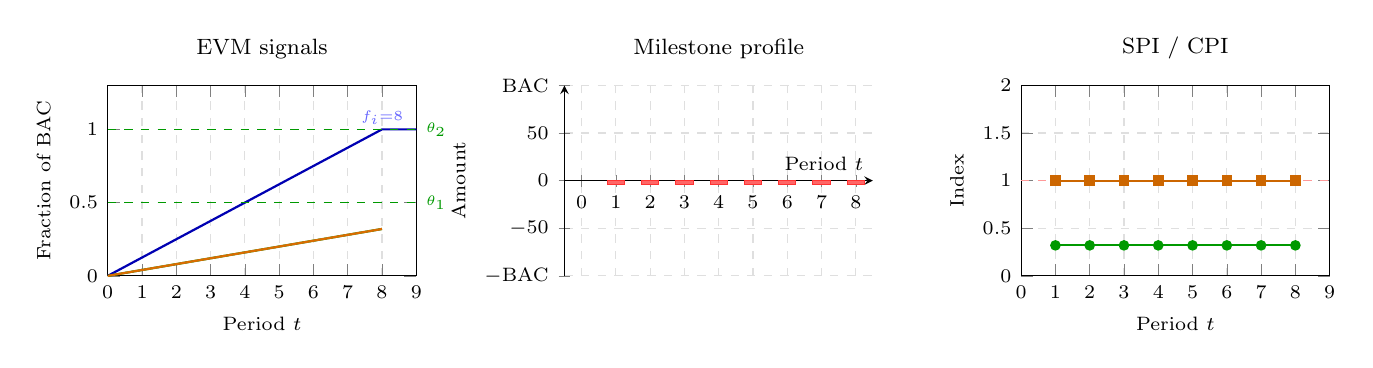
\begin{tikzpicture}[font=\footnotesize]
\begin{scope}
\begin{axis}[
    name=evmspe_p1,
    width=5.5cm, height=4.0cm,
    title={\footnotesize EVM signals},
    xlabel={Period $t$}, ylabel={Fraction of $\BAC$},
    xmin=0, xmax=9, ymin=0, ymax=1.30,
    xtick={0,1,2,3,4,5,6,7,8,9},
    ytick={0,0.5,1},
    grid=major, grid style={dashed,gray!25},
    tick label style={font=\scriptsize},
    label style={font=\scriptsize}, title style={font=\scriptsize},
    clip=false,
  ]
  \addplot[thick,blue!70!black] coordinates {(0,0) (1,0.125) (2,0.25) (3,0.375) (4,0.5) (5,0.625) (6,0.75) (7,0.875) (8,1) (9,1)};
  \addplot[thick,green!55!black] coordinates {(0,0) (1,0.04) (2,0.08) (3,0.12) (4,0.16) (5,0.2) (6,0.24) (7,0.28) (8,0.32)};
  \addplot[thick,orange!85!black] coordinates {(0,0) (1,0.04) (2,0.08) (3,0.12) (4,0.16) (5,0.2) (6,0.24) (7,0.28) (8,0.32)};
  \draw[green!60!black,dashed,thin] (axis cs:0,0.5)--(axis cs:9,0.5) node[right,green!60!black,font=\tiny] {$\theta_{1}$};
  \draw[green!60!black,dashed,thin] (axis cs:0,1)--(axis cs:9,1) node[right,green!60!black,font=\tiny] {$\theta_{2}$};
  \node[font=\tiny,blue!60] at (axis cs:8,1.08) {$f_i{=}8$};
\end{axis}
\end{scope}

\begin{scope}[xshift=5.8cm]
\begin{axis}[
    name=msspe_p1,
    width=5.5cm, height=4.0cm,
    title={\footnotesize Milestone profile},
    xlabel={Period $t$}, ylabel={Amount},
    xmin=-0.5, xmax=8.5, ymin=-100, ymax=100,
    xtick={0,1,2,3,4,5,6,7,8},
    ytick={-100,-50,0,50,100},
    yticklabels={$-\BAC$,$-50$,$0$,$50$,$\BAC$},
    grid=major, grid style={dashed,gray!25},
    tick label style={font=\scriptsize},
    label style={font=\scriptsize}, title style={font=\scriptsize},
    axis x line=center, axis y line=left,
    clip=false,
  ]
  \addplot[ybar,bar width=0.22cm,fill=red!60,draw=red!80] coordinates {(1,-4) (2,-4) (3,-4) (4,-4) (5,-4) (6,-4) (7,-4) (8,-4)};
\end{axis}
\end{scope}

\begin{scope}[xshift=11.6cm]
\begin{axis}[
    name=spicpispe_p1,
    width=5.5cm, height=4.0cm,
    title={\footnotesize SPI / CPI},
    xlabel={Period $t$}, ylabel={Index},
    xmin=0, xmax=9, ymin=0, ymax=2,
    xtick={0,1,2,3,4,5,6,7,8,9},
    ytick={0,0.5,1,1.5,2},
    grid=major, grid style={dashed,gray!25},
    tick label style={font=\scriptsize},
    label style={font=\scriptsize}, title style={font=\scriptsize},
    clip=false,
  ]
  \draw[red!40,dashed,thin] (axis cs:0,1)--(axis cs:9,1);
  \addplot[thick,green!60!black,mark=*,mark size=1.5pt] coordinates {(1,0.32) (2,0.32) (3,0.32) (4,0.32) (5,0.32) (6,0.32) (7,0.32) (8,0.32)};
  \addplot[thick,orange!80!black,mark=square*,mark size=1.5pt] coordinates {(1,1) (2,1) (3,1) (4,1) (5,1) (6,1) (7,1) (8,1)};
\end{axis}
\end{scope}

\end{tikzpicture}

\caption{SP-E project view (single-project). Outcome: \texttt{active}.}
\label{fig:spe_project}
\end{figure}

\begin{figure}[htbp]
\centering
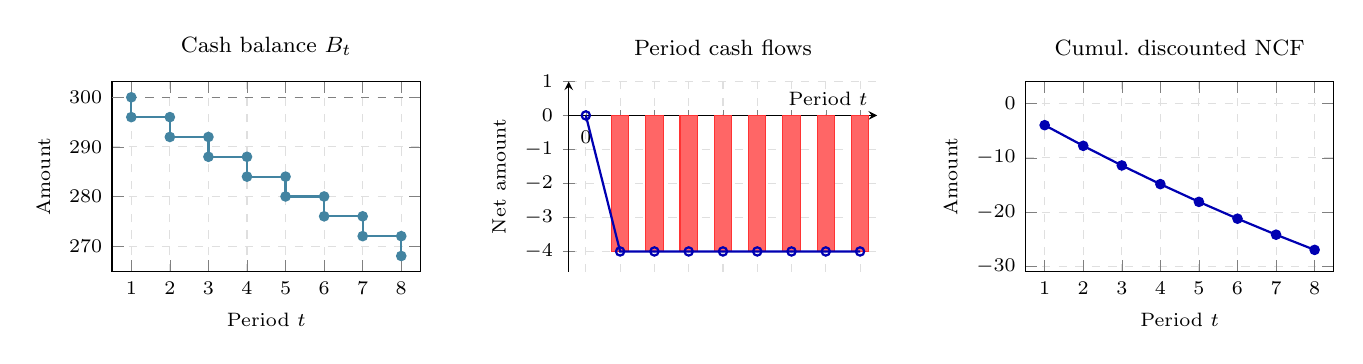
\begin{tikzpicture}[font=\footnotesize]
\begin{scope}
\begin{axis}[
    width=5.5cm, height=4.0cm,
    title={\footnotesize Cash balance $B_t$},
    xlabel={Period $t$}, ylabel={Amount},
    xmin=0.5, xmax=8.5,
    ymin=264.8, ymax=303.2,
    xtick={1,2,3,4,5,6,7,8},
    ytick={270,280,290,300},
    grid=major, grid style={dashed,gray!25},
    tick label style={font=\scriptsize},
    label style={font=\scriptsize}, title style={font=\scriptsize},
  ]
  \addplot[thick,cyan!60!black,mark=*,mark size=1.5pt] coordinates {(1,300) (1,296) (2,296) (2,292) (3,292) (3,288) (4,288) (4,284) (5,284) (5,280) (6,280) (6,276) (7,276) (7,272) (8,272) (8,268)};
  \draw[dashed,gray] (axis cs:0.5,300)--(axis cs:8.5,300) node[right,font=\tiny,gray] {$B_1$};
\end{axis}
\end{scope}

\begin{scope}[xshift=5.8cm]
\begin{axis}[
    width=5.5cm, height=4.0cm,
    title={\footnotesize Period cash flows},
    xlabel={Period $t$}, ylabel={Net amount},
    xmin=-0.5, xmax=8.5,
    ymin=-4.6, ymax=1,
    xtick={0,1,2,3,4,5,6,7,8},
    ytick={-4,-3,-2,-1,0,1},
    grid=major, grid style={dashed,gray!25},
    tick label style={font=\scriptsize},
    label style={font=\scriptsize}, title style={font=\scriptsize},
    axis x line=center, axis y line=left,
    clip=false,
  ]
  \addplot[ybar,bar width=0.22cm,fill=red!60,draw=red!80] coordinates {(1,-4) (2,-4) (3,-4) (4,-4) (5,-4) (6,-4) (7,-4) (8,-4)};
  \addplot[thick,blue!70!black,mark=o,mark size=1.5pt] coordinates {(0,0) (1,-4) (2,-4) (3,-4) (4,-4) (5,-4) (6,-4) (7,-4) (8,-4)};
\end{axis}
\end{scope}

\begin{scope}[xshift=11.6cm]
\begin{axis}[
    width=5.5cm, height=4.0cm,
    title={\footnotesize Cumul.\ discounted NCF},
    xlabel={Period $t$}, ylabel={Amount},
    xmin=0.5, xmax=8.5,
    ymin=-30.965, ymax=4.039,
    xtick={1,2,3,4,5,6,7,8},
    ytick={-30,-20,-10,0},
    grid=major, grid style={dashed,gray!25},
    tick label style={font=\scriptsize},
    label style={font=\scriptsize}, title style={font=\scriptsize},
  ]
  \addplot[thick,blue!70!black,mark=*,mark size=1.5pt] coordinates {(1,-4) (2,-7.8) (3,-11.41) (4,-14.839) (5,-18.098) (6,-21.193) (7,-24.133) (8,-26.926)};
\end{axis}
\end{scope}

\end{tikzpicture}
\caption{SP-E portfolio view.}
\label{fig:spe_portfolio}
\end{figure}

\newpage

\subsection*{SP-F  (Group~G5)}
\begin{center}
\begin{tabular}{ll}
\toprule
$n$,\;$H$ & $1$,\;$20$ \\
$\BAC,\;CP$ & $100,\;100$ \\
$s_i,\;f_i,\;D^{\mathrm{plan}}$ & $1,\;20,\;20$ \\
$\bar\eta$ & $0.5$ \\
$M,\;\theta$ & $2,\;(0.5,1)$ \\
$\phi,\;e_{i,j}$ & $(0.5,0.5),\;(1,20)$ \\
$\mu,\;\Omega,\;\tau^{\mathrm{tol}}$ & $0.05,\;1,\;3$ \\
$B_1,\;\gamma$ & $500,\;0.95$ \\
Outcome & \texttt{active} \\
\bottomrule
\end{tabular}
\end{center}

\begin{center}
\begin{tabular}{rrrrrrrrrrl}
\toprule
$t$ & $x$ & $P$ & BCWS & BCWP & ACWP & SPI & CPI & $\tau$ & MS & $R_{\mathrm{net}}$\\
\midrule
1 & 20 & 0.1 & 0.05 & 0.1 & 0.2 & 2 & 0.5 & 3 & \texttt{---} & 0 \\
2 & 20 & 0.2 & 0.1 & 0.2 & 0.4 & 2 & 0.5 & 3 & \texttt{---} & 0 \\
3 & 20 & 0.3 & 0.15 & 0.3 & 0.6 & 2 & 0.5 & 3 & \texttt{---} & 0 \\
4 & 20 & 0.4 & 0.2 & 0.4 & 0.8 & 2 & 0.5 & 3 & \texttt{---} & 0 \\
5 & 20 & 0.5 & 0.25 & 0.5 & 1 & 2 & 0.5 & 3 & \texttt{1} & 50 \\
6 & 20 & 0.6 & 0.3 & 0.6 & 1.2 & 2 & 0.5 & 3 & \texttt{---} & 0 \\
7 & 20 & 0.7 & 0.35 & 0.7 & 1.4 & 2 & 0.5 & 3 & \texttt{---} & 0 \\
8 & 20 & 0.8 & 0.4 & 0.8 & 1.6 & 2 & 0.5 & 3 & \texttt{---} & 0 \\
9 & 20 & 0.9 & 0.45 & 0.9 & 1.8 & 2 & 0.5 & 3 & \texttt{---} & 0 \\
10 & 20 & 1 & 0.5 & 1 & 2 & 2 & 0.5 & 3 & \texttt{---} & 0 \\
11 & 20 & 1 & 0.55 & 1 & 2.2 & 1.818 & 0.455 & 3 & \texttt{---} & 0 \\
12 & 20 & 1 & 0.6 & 1 & 2.4 & 1.667 & 0.417 & 3 & \texttt{---} & 0 \\
13 & 20 & 1 & 0.65 & 1 & 2.6 & 1.538 & 0.385 & 3 & \texttt{---} & 0 \\
14 & 20 & 1 & 0.7 & 1 & 2.8 & 1.429 & 0.357 & 3 & \texttt{---} & 0 \\
15 & 20 & 1 & 0.75 & 1 & 3 & 1.333 & 0.333 & 3 & \texttt{---} & 0 \\
16 & 20 & 1 & 0.8 & 1 & 3.2 & 1.25 & 0.312 & 3 & \texttt{---} & 0 \\
17 & 20 & 1 & 0.85 & 1 & 3.4 & 1.176 & 0.294 & 3 & \texttt{---} & 0 \\
18 & 20 & 1 & 0.9 & 1 & 3.6 & 1.111 & 0.278 & 3 & \texttt{---} & 0 \\
19 & 20 & 1 & 0.95 & 1 & 3.8 & 1.053 & 0.263 & 3 & \texttt{---} & 0 \\
20 & 20 & 1 & 1 & 1 & 4 & 1 & 0.25 & 3 & \texttt{2} & 50 \\
\bottomrule
\end{tabular}
\end{center}
\paragraph{Portfolio strip.}
\begin{center}
\begin{tabular}{rrrrrrr}
\toprule
$t$ & $B_t$ & $\Sigma\mathrm{In}$ & $\Sigma\mathrm{Out}$ & $\Sigma\mathrm{Net}$ & $\gamma^{t-1}\mathrm{Net}$ & $Z_t^{\mathrm{cum}}$\\
\midrule
1 & 480 & 0 & 20 & -20 & -20 & -20 \\
2 & 460 & 0 & 20 & -20 & -19 & -39 \\
3 & 440 & 0 & 20 & -20 & -18.05 & -57.05 \\
4 & 420 & 0 & 20 & -20 & -17.148 & -74.198 \\
5 & 450 & 50 & 20 & 30 & 24.435 & -49.762 \\
6 & 430 & 0 & 20 & -20 & -15.476 & -65.238 \\
7 & 410 & 0 & 20 & -20 & -14.702 & -79.94 \\
8 & 390 & 0 & 20 & -20 & -13.967 & -93.907 \\
9 & 370 & 0 & 20 & -20 & -13.268 & -107.175 \\
10 & 350 & 0 & 20 & -20 & -12.605 & -119.78 \\
11 & 330 & 0 & 20 & -20 & -11.975 & -131.755 \\
12 & 310 & 0 & 20 & -20 & -11.376 & -143.131 \\
13 & 290 & 0 & 20 & -20 & -10.807 & -153.938 \\
14 & 270 & 0 & 20 & -20 & -10.267 & -164.205 \\
15 & 250 & 0 & 20 & -20 & -9.754 & -173.958 \\
16 & 230 & 0 & 20 & -20 & -9.266 & -183.224 \\
17 & 210 & 0 & 20 & -20 & -8.803 & -192.027 \\
18 & 190 & 0 & 20 & -20 & -8.362 & -200.389 \\
19 & 170 & 0 & 20 & -20 & -7.944 & -208.333 \\
20 & 200 & 50 & 20 & 30 & 11.321 & -197.013 \\
\bottomrule
\end{tabular}
\end{center}

\begin{figure}[htbp]
\centering
% === Project 1 row for SP-F ===
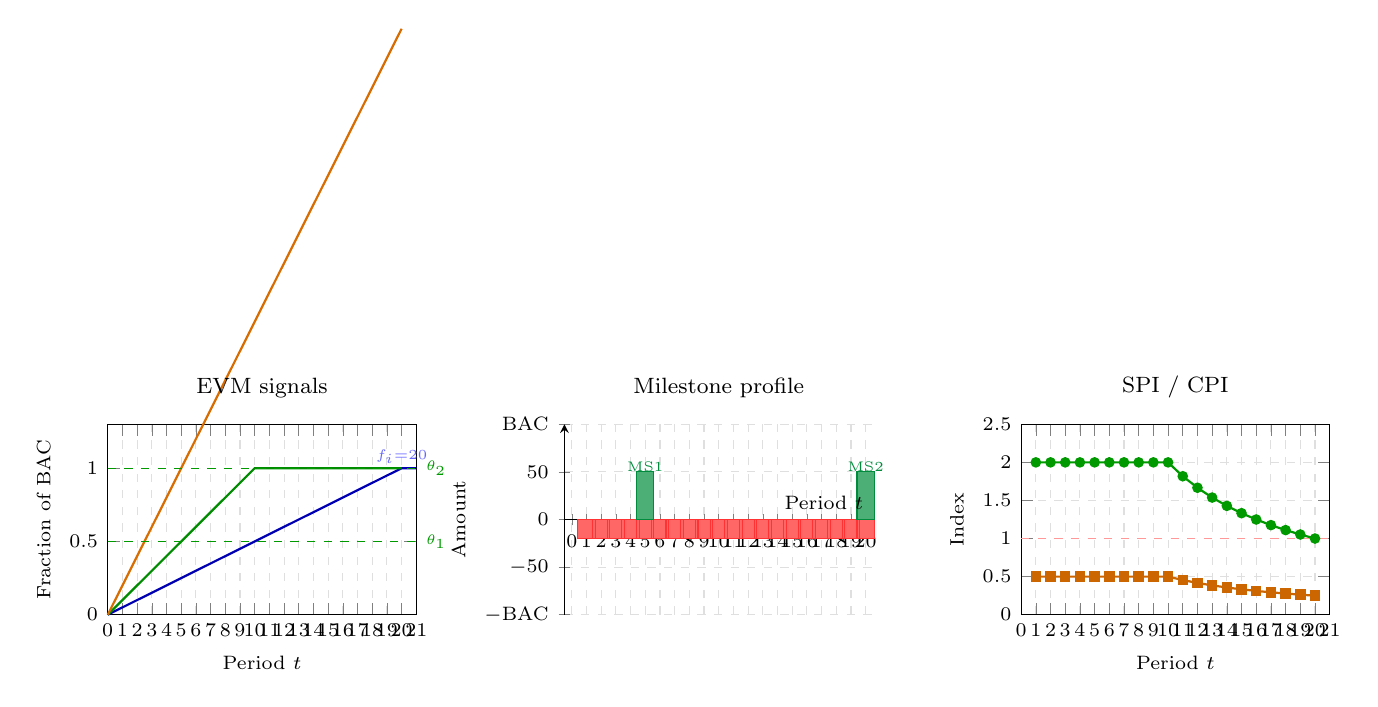
\begin{tikzpicture}[font=\footnotesize]
\begin{scope}
\begin{axis}[
    name=evmspf_p1,
    width=5.5cm, height=4.0cm,
    title={\footnotesize EVM signals},
    xlabel={Period $t$}, ylabel={Fraction of $\BAC$},
    xmin=0, xmax=21, ymin=0, ymax=1.30,
    xtick={0,1,2,3,4,5,6,7,8,9,10,11,12,13,14,15,16,17,18,19,20,21},
    ytick={0,0.5,1},
    grid=major, grid style={dashed,gray!25},
    tick label style={font=\scriptsize},
    label style={font=\scriptsize}, title style={font=\scriptsize},
    clip=false,
  ]
  \addplot[thick,blue!70!black] coordinates {(0,0) (1,0.05) (2,0.1) (3,0.15) (4,0.2) (5,0.25) (6,0.3) (7,0.35) (8,0.4) (9,0.45) (10,0.5) (11,0.55) (12,0.6) (13,0.65) (14,0.7) (15,0.75) (16,0.8) (17,0.85) (18,0.9) (19,0.95) (20,1) (21,1)};
  \addplot[thick,green!55!black] coordinates {(0,0) (1,0.1) (2,0.2) (3,0.3) (4,0.4) (5,0.5) (6,0.6) (7,0.7) (8,0.8) (9,0.9) (10,1) (11,1) (12,1) (13,1) (14,1) (15,1) (16,1) (17,1) (18,1) (19,1) (20,1)};
  \addplot[thick,orange!85!black] coordinates {(0,0) (1,0.2) (2,0.4) (3,0.6) (4,0.8) (5,1) (6,1.2) (7,1.4) (8,1.6) (9,1.8) (10,2) (11,2.2) (12,2.4) (13,2.6) (14,2.8) (15,3) (16,3.2) (17,3.4) (18,3.6) (19,3.8) (20,4)};
  \draw[green!60!black,dashed,thin] (axis cs:0,0.5)--(axis cs:21,0.5) node[right,green!60!black,font=\tiny] {$\theta_{1}$};
  \draw[green!60!black,dashed,thin] (axis cs:0,1)--(axis cs:21,1) node[right,green!60!black,font=\tiny] {$\theta_{2}$};
  \node[font=\tiny,blue!60] at (axis cs:20,1.08) {$f_i{=}20$};
\end{axis}
\end{scope}

\begin{scope}[xshift=5.8cm]
\begin{axis}[
    name=msspf_p1,
    width=5.5cm, height=4.0cm,
    title={\footnotesize Milestone profile},
    xlabel={Period $t$}, ylabel={Amount},
    xmin=-0.5, xmax=20.5, ymin=-100, ymax=100,
    xtick={0,1,2,3,4,5,6,7,8,9,10,11,12,13,14,15,16,17,18,19,20},
    ytick={-100,-50,0,50,100},
    yticklabels={$-\BAC$,$-50$,$0$,$50$,$\BAC$},
    grid=major, grid style={dashed,gray!25},
    tick label style={font=\scriptsize},
    label style={font=\scriptsize}, title style={font=\scriptsize},
    axis x line=center, axis y line=left,
    clip=false,
  ]
  \addplot[ybar,bar width=0.22cm,fill=red!60,draw=red!80] coordinates {(1,-20) (2,-20) (3,-20) (4,-20) (5,-20) (6,-20) (7,-20) (8,-20) (9,-20) (10,-20) (11,-20) (12,-20) (13,-20) (14,-20) (15,-20) (16,-20) (17,-20) (18,-20) (19,-20) (20,-20)};
  \addplot[ybar,bar width=0.22cm,fill=msgreen!70,draw=msgreen] coordinates {(5,50) (20,50)};
  \node[font=\tiny,msgreen] at (axis cs:5,55) {MS1};
  \node[font=\tiny,msgreen] at (axis cs:20,55) {MS2};
\end{axis}
\end{scope}

\begin{scope}[xshift=11.6cm]
\begin{axis}[
    name=spicpispf_p1,
    width=5.5cm, height=4.0cm,
    title={\footnotesize SPI / CPI},
    xlabel={Period $t$}, ylabel={Index},
    xmin=0, xmax=21, ymin=0, ymax=2.5,
    xtick={0,1,2,3,4,5,6,7,8,9,10,11,12,13,14,15,16,17,18,19,20,21},
    ytick={0,0.5,1,1.5,2,2.5},
    grid=major, grid style={dashed,gray!25},
    tick label style={font=\scriptsize},
    label style={font=\scriptsize}, title style={font=\scriptsize},
    clip=false,
  ]
  \draw[red!40,dashed,thin] (axis cs:0,1)--(axis cs:21,1);
  \addplot[thick,green!60!black,mark=*,mark size=1.5pt] coordinates {(1,2) (2,2) (3,2) (4,2) (5,2) (6,2) (7,2) (8,2) (9,2) (10,2) (11,1.818) (12,1.667) (13,1.538) (14,1.429) (15,1.333) (16,1.25) (17,1.176) (18,1.111) (19,1.053) (20,1)};
  \addplot[thick,orange!80!black,mark=square*,mark size=1.5pt] coordinates {(1,0.5) (2,0.5) (3,0.5) (4,0.5) (5,0.5) (6,0.5) (7,0.5) (8,0.5) (9,0.5) (10,0.5) (11,0.455) (12,0.417) (13,0.385) (14,0.357) (15,0.333) (16,0.312) (17,0.294) (18,0.278) (19,0.263) (20,0.25)};
\end{axis}
\end{scope}

\end{tikzpicture}

\caption{SP-F project view (single-project). Outcome: \texttt{active}.}
\label{fig:spf_project}
\end{figure}

\begin{figure}[htbp]
\centering
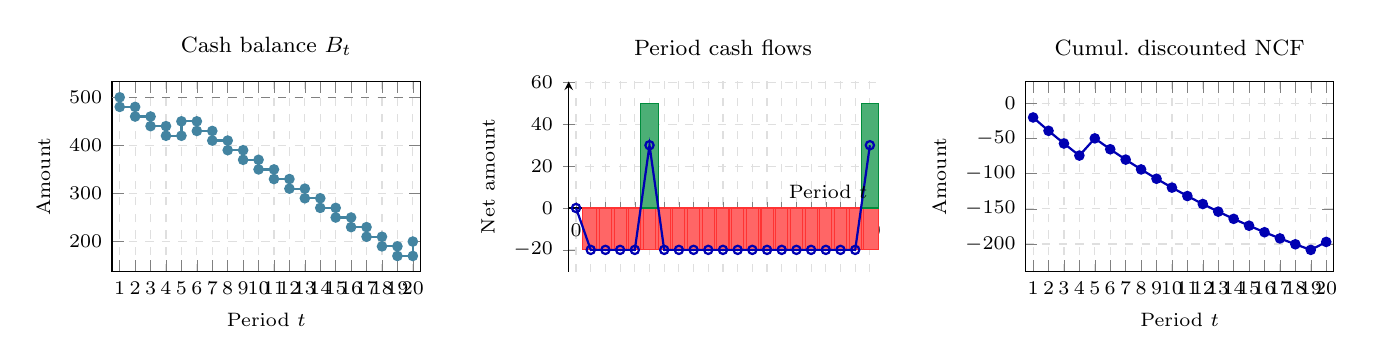
\begin{tikzpicture}[font=\footnotesize]
\begin{scope}
\begin{axis}[
    width=5.5cm, height=4.0cm,
    title={\footnotesize Cash balance $B_t$},
    xlabel={Period $t$}, ylabel={Amount},
    xmin=0.5, xmax=20.5,
    ymin=137, ymax=533,
    xtick={1,2,3,4,5,6,7,8,9,10,11,12,13,14,15,16,17,18,19,20},
    ytick={200,300,400,500},
    grid=major, grid style={dashed,gray!25},
    tick label style={font=\scriptsize},
    label style={font=\scriptsize}, title style={font=\scriptsize},
  ]
  \addplot[thick,cyan!60!black,mark=*,mark size=1.5pt] coordinates {(1,500) (1,480) (2,480) (2,460) (3,460) (3,440) (4,440) (4,420) (5,420) (5,450) (6,450) (6,430) (7,430) (7,410) (8,410) (8,390) (9,390) (9,370) (10,370) (10,350) (11,350) (11,330) (12,330) (12,310) (13,310) (13,290) (14,290) (14,270) (15,270) (15,250) (16,250) (16,230) (17,230) (17,210) (18,210) (18,190) (19,190) (19,170) (20,170) (20,200)};
  \draw[dashed,gray] (axis cs:0.5,500)--(axis cs:20.5,500) node[right,font=\tiny,gray] {$B_1$};
\end{axis}
\end{scope}

\begin{scope}[xshift=5.8cm]
\begin{axis}[
    width=5.5cm, height=4.0cm,
    title={\footnotesize Period cash flows},
    xlabel={Period $t$}, ylabel={Net amount},
    xmin=-0.5, xmax=20.5,
    ymin=-30.5, ymax=60.5,
    xtick={0,1,2,3,4,5,6,7,8,9,10,11,12,13,14,15,16,17,18,19,20},
    ytick={-20,0,20,40,60},
    grid=major, grid style={dashed,gray!25},
    tick label style={font=\scriptsize},
    label style={font=\scriptsize}, title style={font=\scriptsize},
    axis x line=center, axis y line=left,
    clip=false,
  ]
  \addplot[ybar,bar width=0.22cm,fill=red!60,draw=red!80] coordinates {(1,-20) (2,-20) (3,-20) (4,-20) (5,-20) (6,-20) (7,-20) (8,-20) (9,-20) (10,-20) (11,-20) (12,-20) (13,-20) (14,-20) (15,-20) (16,-20) (17,-20) (18,-20) (19,-20) (20,-20)};
  \addplot[ybar,bar width=0.22cm,fill=msgreen!70,draw=msgreen] coordinates {(5,50) (20,50)};
  \addplot[thick,blue!70!black,mark=o,mark size=1.5pt] coordinates {(0,0) (1,-20) (2,-20) (3,-20) (4,-20) (5,30) (6,-20) (7,-20) (8,-20) (9,-20) (10,-20) (11,-20) (12,-20) (13,-20) (14,-20) (15,-20) (16,-20) (17,-20) (18,-20) (19,-20) (20,30)};
\end{axis}
\end{scope}

\begin{scope}[xshift=11.6cm]
\begin{axis}[
    width=5.5cm, height=4.0cm,
    title={\footnotesize Cumul.\ discounted NCF},
    xlabel={Period $t$}, ylabel={Amount},
    xmin=0.5, xmax=20.5,
    ymin=-239.583, ymax=31.25,
    xtick={1,2,3,4,5,6,7,8,9,10,11,12,13,14,15,16,17,18,19,20},
    ytick={-200,-150,-100,-50,0},
    grid=major, grid style={dashed,gray!25},
    tick label style={font=\scriptsize},
    label style={font=\scriptsize}, title style={font=\scriptsize},
  ]
  \addplot[thick,blue!70!black,mark=*,mark size=1.5pt] coordinates {(1,-20) (2,-39) (3,-57.05) (4,-74.198) (5,-49.762) (6,-65.238) (7,-79.94) (8,-93.907) (9,-107.175) (10,-119.78) (11,-131.755) (12,-143.131) (13,-153.938) (14,-164.205) (15,-173.958) (16,-183.224) (17,-192.027) (18,-200.389) (19,-208.333) (20,-197.013)};
\end{axis}
\end{scope}

\end{tikzpicture}
\caption{SP-F portfolio view.}
\label{fig:spf_portfolio}
\end{figure}

\newpage

\subsection*{SP-G  (Group~G5)}
\begin{center}
\begin{tabular}{ll}
\toprule
$n$,\;$H$ & $1$,\;$12$ \\
$\BAC,\;CP$ & $100,\;100$ \\
$s_i,\;f_i,\;D^{\mathrm{plan}}$ & $1,\;12,\;12$ \\
$\bar\eta$ & $1$ \\
$M,\;\theta$ & $2,\;(0.5,1)$ \\
$\phi,\;e_{i,j}$ & $(0.5,0.5),\;(1,12)$ \\
$\mu,\;\Omega,\;\tau^{\mathrm{tol}}$ & $0.5,\;1,\;3$ \\
$B_1,\;\gamma$ & $300,\;0.95$ \\
Outcome & \texttt{active} \\
\bottomrule
\end{tabular}
\end{center}

\begin{center}
\begin{tabular}{rrrrrrrrrrl}
\toprule
$t$ & $x$ & $P$ & BCWS & BCWP & ACWP & SPI & CPI & $\tau$ & MS & $R_{\mathrm{net}}$\\
\midrule
1 & 10 & 0.03 & 0.083 & 0.03 & 0.1 & 0.36 & 0.3 & 2 & \texttt{---} & 0 \\
2 & 10 & 0.06 & 0.167 & 0.06 & 0.2 & 0.36 & 0.3 & 1 & \texttt{---} & 0 \\
3 & 80 & 0.86 & 0.25 & 0.86 & 1 & 3.44 & 0.86 & 3 & \texttt{1} & 50 \\
4 & 10 & 0.89 & 0.333 & 0.89 & 1.1 & 2.67 & 0.809 & 3 & \texttt{---} & 0 \\
5 & 10 & 0.92 & 0.417 & 0.92 & 1.2 & 2.208 & 0.767 & 3 & \texttt{---} & 0 \\
6 & 10 & 0.95 & 0.5 & 0.95 & 1.3 & 1.9 & 0.731 & 3 & \texttt{---} & 0 \\
7 & 10 & 0.98 & 0.583 & 0.98 & 1.4 & 1.68 & 0.7 & 3 & \texttt{---} & 0 \\
8 & 10 & 1 & 0.667 & 1 & 1.5 & 1.5 & 0.667 & 3 & \texttt{---} & 0 \\
9 & 10 & 1 & 0.75 & 1 & 1.6 & 1.333 & 0.625 & 3 & \texttt{---} & 0 \\
10 & 10 & 1 & 0.833 & 1 & 1.7 & 1.2 & 0.588 & 3 & \texttt{---} & 0 \\
11 & 10 & 1 & 0.917 & 1 & 1.8 & 1.091 & 0.556 & 3 & \texttt{---} & 0 \\
12 & 10 & 1 & 1 & 1 & 1.9 & 1 & 0.526 & 3 & \texttt{2} & 50 \\
\bottomrule
\end{tabular}
\end{center}
\paragraph{Portfolio strip.}
\begin{center}
\begin{tabular}{rrrrrrr}
\toprule
$t$ & $B_t$ & $\Sigma\mathrm{In}$ & $\Sigma\mathrm{Out}$ & $\Sigma\mathrm{Net}$ & $\gamma^{t-1}\mathrm{Net}$ & $Z_t^{\mathrm{cum}}$\\
\midrule
1 & 290 & 0 & 10 & -10 & -10 & -10 \\
2 & 280 & 0 & 10 & -10 & -9.5 & -19.5 \\
3 & 250 & 50 & 80 & -30 & -27.075 & -46.575 \\
4 & 240 & 0 & 10 & -10 & -8.574 & -55.149 \\
5 & 230 & 0 & 10 & -10 & -8.145 & -63.294 \\
6 & 220 & 0 & 10 & -10 & -7.738 & -71.032 \\
7 & 210 & 0 & 10 & -10 & -7.351 & -78.383 \\
8 & 200 & 0 & 10 & -10 & -6.983 & -85.366 \\
9 & 190 & 0 & 10 & -10 & -6.634 & -92 \\
10 & 180 & 0 & 10 & -10 & -6.302 & -98.303 \\
11 & 170 & 0 & 10 & -10 & -5.987 & -104.29 \\
12 & 210 & 50 & 10 & 40 & 22.752 & -81.538 \\
\bottomrule
\end{tabular}
\end{center}

\begin{figure}[htbp]
\centering
% === Project 1 row for SP-G ===
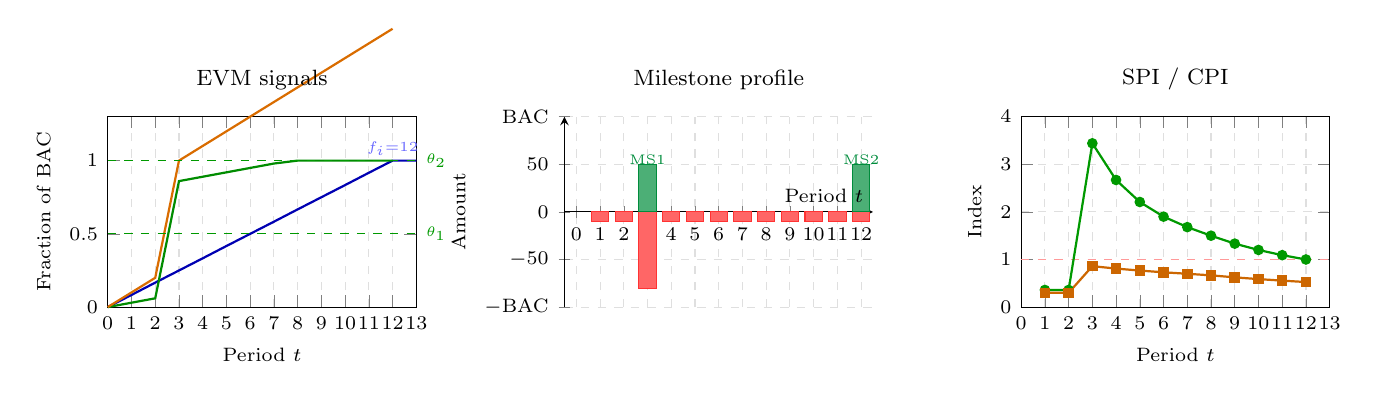
\begin{tikzpicture}[font=\footnotesize]
\begin{scope}
\begin{axis}[
    name=evmspg_p1,
    width=5.5cm, height=4.0cm,
    title={\footnotesize EVM signals},
    xlabel={Period $t$}, ylabel={Fraction of $\BAC$},
    xmin=0, xmax=13, ymin=0, ymax=1.30,
    xtick={0,1,2,3,4,5,6,7,8,9,10,11,12,13},
    ytick={0,0.5,1},
    grid=major, grid style={dashed,gray!25},
    tick label style={font=\scriptsize},
    label style={font=\scriptsize}, title style={font=\scriptsize},
    clip=false,
  ]
  \addplot[thick,blue!70!black] coordinates {(0,0) (1,0.083) (2,0.167) (3,0.25) (4,0.333) (5,0.417) (6,0.5) (7,0.583) (8,0.667) (9,0.75) (10,0.833) (11,0.917) (12,1) (13,1)};
  \addplot[thick,green!55!black] coordinates {(0,0) (1,0.03) (2,0.06) (3,0.86) (4,0.89) (5,0.92) (6,0.95) (7,0.98) (8,1) (9,1) (10,1) (11,1) (12,1)};
  \addplot[thick,orange!85!black] coordinates {(0,0) (1,0.1) (2,0.2) (3,1) (4,1.1) (5,1.2) (6,1.3) (7,1.4) (8,1.5) (9,1.6) (10,1.7) (11,1.8) (12,1.9)};
  \draw[green!60!black,dashed,thin] (axis cs:0,0.5)--(axis cs:13,0.5) node[right,green!60!black,font=\tiny] {$\theta_{1}$};
  \draw[green!60!black,dashed,thin] (axis cs:0,1)--(axis cs:13,1) node[right,green!60!black,font=\tiny] {$\theta_{2}$};
  \node[font=\tiny,blue!60] at (axis cs:12,1.08) {$f_i{=}12$};
\end{axis}
\end{scope}

\begin{scope}[xshift=5.8cm]
\begin{axis}[
    name=msspg_p1,
    width=5.5cm, height=4.0cm,
    title={\footnotesize Milestone profile},
    xlabel={Period $t$}, ylabel={Amount},
    xmin=-0.5, xmax=12.5, ymin=-100, ymax=100,
    xtick={0,1,2,3,4,5,6,7,8,9,10,11,12},
    ytick={-100,-50,0,50,100},
    yticklabels={$-\BAC$,$-50$,$0$,$50$,$\BAC$},
    grid=major, grid style={dashed,gray!25},
    tick label style={font=\scriptsize},
    label style={font=\scriptsize}, title style={font=\scriptsize},
    axis x line=center, axis y line=left,
    clip=false,
  ]
  \addplot[ybar,bar width=0.22cm,fill=red!60,draw=red!80] coordinates {(1,-10) (2,-10) (3,-80) (4,-10) (5,-10) (6,-10) (7,-10) (8,-10) (9,-10) (10,-10) (11,-10) (12,-10)};
  \addplot[ybar,bar width=0.22cm,fill=msgreen!70,draw=msgreen] coordinates {(3,50) (12,50)};
  \node[font=\tiny,msgreen] at (axis cs:3,55) {MS1};
  \node[font=\tiny,msgreen] at (axis cs:12,55) {MS2};
\end{axis}
\end{scope}

\begin{scope}[xshift=11.6cm]
\begin{axis}[
    name=spicpispg_p1,
    width=5.5cm, height=4.0cm,
    title={\footnotesize SPI / CPI},
    xlabel={Period $t$}, ylabel={Index},
    xmin=0, xmax=13, ymin=0, ymax=4,
    xtick={0,1,2,3,4,5,6,7,8,9,10,11,12,13},
    ytick={0,1,2,3,4},
    grid=major, grid style={dashed,gray!25},
    tick label style={font=\scriptsize},
    label style={font=\scriptsize}, title style={font=\scriptsize},
    clip=false,
  ]
  \draw[red!40,dashed,thin] (axis cs:0,1)--(axis cs:13,1);
  \addplot[thick,green!60!black,mark=*,mark size=1.5pt] coordinates {(1,0.36) (2,0.36) (3,3.44) (4,2.67) (5,2.208) (6,1.9) (7,1.68) (8,1.5) (9,1.333) (10,1.2) (11,1.091) (12,1)};
  \addplot[thick,orange!80!black,mark=square*,mark size=1.5pt] coordinates {(1,0.3) (2,0.3) (3,0.86) (4,0.809) (5,0.767) (6,0.731) (7,0.7) (8,0.667) (9,0.625) (10,0.588) (11,0.556) (12,0.526)};
\end{axis}
\end{scope}

\end{tikzpicture}

\caption{SP-G project view (single-project). Outcome: \texttt{active}.}
\label{fig:spg_project}
\end{figure}

\begin{figure}[htbp]
\centering
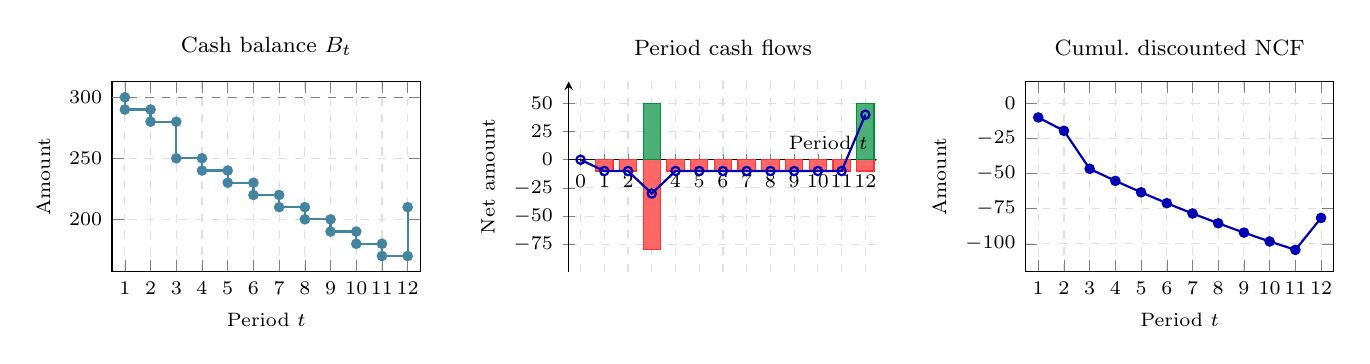
\begin{tikzpicture}[font=\footnotesize]
\begin{scope}
\begin{axis}[
    width=5.5cm, height=4.0cm,
    title={\footnotesize Cash balance $B_t$},
    xlabel={Period $t$}, ylabel={Amount},
    xmin=0.5, xmax=12.5,
    ymin=157, ymax=313,
    xtick={1,2,3,4,5,6,7,8,9,10,11,12},
    ytick={200,250,300},
    grid=major, grid style={dashed,gray!25},
    tick label style={font=\scriptsize},
    label style={font=\scriptsize}, title style={font=\scriptsize},
  ]
  \addplot[thick,cyan!60!black,mark=*,mark size=1.5pt] coordinates {(1,300) (1,290) (2,290) (2,280) (3,280) (3,250) (4,250) (4,240) (5,240) (5,230) (6,230) (6,220) (7,220) (7,210) (8,210) (8,200) (9,200) (9,190) (10,190) (10,180) (11,180) (11,170) (12,170) (12,210)};
  \draw[dashed,gray] (axis cs:0.5,300)--(axis cs:12.5,300) node[right,font=\tiny,gray] {$B_1$};
\end{axis}
\end{scope}

\begin{scope}[xshift=5.8cm]
\begin{axis}[
    width=5.5cm, height=4.0cm,
    title={\footnotesize Period cash flows},
    xlabel={Period $t$}, ylabel={Net amount},
    xmin=-0.5, xmax=12.5,
    ymin=-99.5, ymax=69.5,
    xtick={0,1,2,3,4,5,6,7,8,9,10,11,12},
    ytick={-75,-50,-25,0,25,50},
    grid=major, grid style={dashed,gray!25},
    tick label style={font=\scriptsize},
    label style={font=\scriptsize}, title style={font=\scriptsize},
    axis x line=center, axis y line=left,
    clip=false,
  ]
  \addplot[ybar,bar width=0.22cm,fill=red!60,draw=red!80] coordinates {(1,-10) (2,-10) (3,-80) (4,-10) (5,-10) (6,-10) (7,-10) (8,-10) (9,-10) (10,-10) (11,-10) (12,-10)};
  \addplot[ybar,bar width=0.22cm,fill=msgreen!70,draw=msgreen] coordinates {(3,50) (12,50)};
  \addplot[thick,blue!70!black,mark=o,mark size=1.5pt] coordinates {(0,0) (1,-10) (2,-10) (3,-30) (4,-10) (5,-10) (6,-10) (7,-10) (8,-10) (9,-10) (10,-10) (11,-10) (12,40)};
\end{axis}
\end{scope}

\begin{scope}[xshift=11.6cm]
\begin{axis}[
    width=5.5cm, height=4.0cm,
    title={\footnotesize Cumul.\ discounted NCF},
    xlabel={Period $t$}, ylabel={Amount},
    xmin=0.5, xmax=12.5,
    ymin=-119.933, ymax=15.643,
    xtick={1,2,3,4,5,6,7,8,9,10,11,12},
    ytick={-100,-75,-50,-25,0},
    grid=major, grid style={dashed,gray!25},
    tick label style={font=\scriptsize},
    label style={font=\scriptsize}, title style={font=\scriptsize},
  ]
  \addplot[thick,blue!70!black,mark=*,mark size=1.5pt] coordinates {(1,-10) (2,-19.5) (3,-46.575) (4,-55.149) (5,-63.294) (6,-71.032) (7,-78.383) (8,-85.366) (9,-92) (10,-98.303) (11,-104.29) (12,-81.538)};
\end{axis}
\end{scope}

\end{tikzpicture}
\caption{SP-G portfolio view.}
\label{fig:spg_portfolio}
\end{figure}

\newpage


\subsection*{Group 6: Forced and Starvation Termination}

\subsection*{SP-5  (Group~G6)}
\begin{center}
\begin{tabular}{ll}
\toprule
$n$,\;$H$ & $1$,\;$6$ \\
$\BAC,\;CP$ & $100,\;100$ \\
$s_i,\;f_i,\;D^{\mathrm{plan}}$ & $1,\;6,\;6$ \\
$\bar\eta$ & $0$ \\
$\alpha,\;A$ & $0.2,\;20$ \\
$M,\;\theta$ & $2,\;(0.5,1)$ \\
$\phi,\;e_{i,j}$ & $(0.5,0.5),\;(1,4)$ \\
$\mu,\;\Omega,\;\tau^{\mathrm{tol}}$ & $0.1,\;1,\;3$ \\
$B_1,\;\gamma$ & $300,\;0.95$ \\
$Z^*$ & $2.85$ \\
Outcome & \texttt{terminated} \\
\bottomrule
\end{tabular}
\end{center}

\begin{center}
\begin{tabular}{rrrrrrrrrrl}
\toprule
$t$ & $x$ & $P$ & BCWS & BCWP & ACWP & SPI & CPI & $\tau$ & MS & $R_{\mathrm{net}}$\\
\midrule
1 & 0 & 0 & 0.167 & 0 & 0 & 0 & 1 & 3 & \texttt{---} & 0 \\
2 & 0 & 0 & 0.333 & 0 & 0 & 0 & 1 & 3 & \texttt{---} & 0 \\
3 & 0 & 0 & 0.5 & 0 & 0 & 0 & 1 & 3 & \texttt{---} & 0 \\
4 & 0 & 0 & 0.667 & 0 & 0 & 0 & 1 & 3 & \texttt{---} & -20 \\
\bottomrule
\end{tabular}
\end{center}
\paragraph{Portfolio strip.}
\begin{center}
\begin{tabular}{rrrrrrr}
\toprule
$t$ & $B_t$ & $\Sigma\mathrm{In}$ & $\Sigma\mathrm{Out}$ & $\Sigma\mathrm{Net}$ & $\gamma^{t-1}\mathrm{Net}$ & $Z_t^{\mathrm{cum}}$\\
\midrule
1 & 320 & 0 & 0 & 0 & 0 & 20 \\
2 & 320 & 0 & 0 & 0 & 0 & 20 \\
3 & 320 & 0 & 0 & 0 & 0 & 20 \\
4 & 300 & -20 & 0 & -20 & -17.148 & 2.853 \\
5 & 300 & 0 & 0 & 0 & 0 & 2.853 \\
6 & 300 & 0 & 0 & 0 & 0 & 2.853 \\
\bottomrule
\end{tabular}
\end{center}

\begin{figure}[htbp]
\centering
% === Project 1 row for SP-5 ===
\begin{tikzpicture}[font=\footnotesize]
\begin{scope}
\begin{axis}[
    name=evmsp5_p1,
    width=5.5cm, height=4.0cm,
    title={\footnotesize EVM signals},
    xlabel={Period $t$}, ylabel={Fraction of $\BAC$},
    xmin=0, xmax=7, ymin=0, ymax=1.30,
    xtick={0,1,2,3,4,5,6,7},
    ytick={0,0.5,1},
    grid=major, grid style={dashed,gray!25},
    tick label style={font=\scriptsize},
    label style={font=\scriptsize}, title style={font=\scriptsize},
    clip=false,
  ]
  \addplot[thick,blue!70!black] coordinates {(0,0) (1,0.167) (2,0.333) (3,0.5) (4,0.667) (7,0.667)};
  \addplot[thick,green!55!black] coordinates {(0,0) (1,0) (2,0) (3,0) (4,0)};
  \addplot[thick,orange!85!black] coordinates {(0,0) (1,0) (2,0) (3,0) (4,0)};
  \draw[green!60!black,dashed,thin] (axis cs:0,0.5)--(axis cs:7,0.5) node[right,green!60!black,font=\tiny] {$\theta_{1}$};
  \draw[green!60!black,dashed,thin] (axis cs:0,1)--(axis cs:7,1) node[right,green!60!black,font=\tiny] {$\theta_{2}$};
  \node[font=\tiny,blue!60] at (axis cs:6,1.08) {$f_i{=}6$};
  \draw[red!80!black,dashed,thick] (axis cs:4,0)--(axis cs:4,1.30) node[above,font=\tiny,red!80!black] {Term.\,$t=4$};
\end{axis}
\end{scope}

\begin{scope}[xshift=5.8cm]
\begin{axis}[
    name=mssp5_p1,
    width=5.5cm, height=4.0cm,
    title={\footnotesize Milestone profile},
    xlabel={Period $t$}, ylabel={Amount},
    xmin=-0.5, xmax=6.5, ymin=-100, ymax=100,
    xtick={0,1,2,3,4,5,6},
    ytick={-100,-50,0,50,100},
    yticklabels={$-\BAC$,$-50$,$0$,$50$,$\BAC$},
    grid=major, grid style={dashed,gray!25},
    tick label style={font=\scriptsize},
    label style={font=\scriptsize}, title style={font=\scriptsize},
    axis x line=center, axis y line=left,
    clip=false,
  ]
  \addplot[ybar,bar width=0.22cm,fill=red!60,draw=red!80] coordinates {(4,-20)};
  \addplot[ybar,bar width=0.22cm,fill=msgreen!70,draw=msgreen] coordinates {(0,20)};
  \node[font=\tiny,msgreen] at (axis cs:0,25) {$A_i$};
\end{axis}
\end{scope}

\begin{scope}[xshift=11.6cm]
\begin{axis}[
    name=spicpisp5_p1,
    width=5.5cm, height=4.0cm,
    title={\footnotesize SPI / CPI},
    xlabel={Period $t$}, ylabel={Index},
    xmin=0, xmax=7, ymin=0, ymax=2,
    xtick={0,1,2,3,4,5,6,7},
    ytick={0,0.5,1,1.5,2},
    grid=major, grid style={dashed,gray!25},
    tick label style={font=\scriptsize},
    label style={font=\scriptsize}, title style={font=\scriptsize},
    clip=false,
  ]
  \draw[red!40,dashed,thin] (axis cs:0,1)--(axis cs:7,1);
  \addplot[thick,green!60!black,mark=*,mark size=1.5pt] coordinates {(1,0) (2,0) (3,0) (4,0)};
  \addplot[thick,orange!80!black,mark=square*,mark size=1.5pt] coordinates {(1,1) (2,1) (3,1) (4,1)};
\end{axis}
\end{scope}

\end{tikzpicture}

\caption{SP-5 project view (single-project). Outcome: \texttt{terminated}. $Z^*=2.85$.}
\label{fig:sp5_project}
\end{figure}

\begin{figure}[htbp]
\centering
\begin{tikzpicture}[font=\footnotesize]
\begin{scope}
\begin{axis}[
    width=5.5cm, height=4.0cm,
    title={\footnotesize Cash balance $B_t$},
    xlabel={Period $t$}, ylabel={Amount},
    xmin=0.5, xmax=6.5,
    ymin=298, ymax=322,
    xtick={1,2,3,4,5,6},
    ytick={300,305,310,315,320},
    grid=major, grid style={dashed,gray!25},
    tick label style={font=\scriptsize},
    label style={font=\scriptsize}, title style={font=\scriptsize},
  ]
  \addplot[thick,cyan!60!black,mark=*,mark size=1.5pt] coordinates {(1,320) (1,320) (2,320) (2,320) (3,320) (3,320) (4,320) (4,300) (5,300) (5,300) (6,300) (6,300)};
  \draw[dashed,gray] (axis cs:0.5,300)--(axis cs:6.5,300) node[right,font=\tiny,gray] {$B_1$};
\end{axis}
\end{scope}

\begin{scope}[xshift=5.8cm]
\begin{axis}[
    width=5.5cm, height=4.0cm,
    title={\footnotesize Period cash flows},
    xlabel={Period $t$}, ylabel={Net amount},
    xmin=-0.5, xmax=6.5,
    ymin=-3, ymax=23,
    xtick={0,1,2,3,4,5,6},
    ytick={0,5,10,15,20},
    grid=major, grid style={dashed,gray!25},
    tick label style={font=\scriptsize},
    label style={font=\scriptsize}, title style={font=\scriptsize},
    axis x line=center, axis y line=left,
    clip=false,
  ]
  \addplot[ybar,bar width=0.22cm,fill=msgreen!70,draw=msgreen] coordinates {(0,20)};
  \addplot[thick,blue!70!black,mark=o,mark size=1.5pt] coordinates {(0,20) (1,0) (2,0) (3,0) (4,-20) (5,0) (6,0)};
\end{axis}
\end{scope}

\begin{scope}[xshift=11.6cm]
\begin{axis}[
    width=5.5cm, height=4.0cm,
    title={\footnotesize Cumul.\ discounted NCF},
    xlabel={Period $t$}, ylabel={Amount},
    xmin=0.5, xmax=6.5,
    ymin=-3, ymax=23,
    xtick={1,2,3,4,5,6},
    ytick={0,5,10,15,20},
    grid=major, grid style={dashed,gray!25},
    tick label style={font=\scriptsize},
    label style={font=\scriptsize}, title style={font=\scriptsize},
  ]
  \addplot[thick,blue!70!black,mark=*,mark size=1.5pt] coordinates {(1,20) (2,20) (3,20) (4,2.853) (5,2.853) (6,2.853)};
\end{axis}
\end{scope}

\end{tikzpicture}
\caption{SP-5 portfolio view. $Z^*=2.85$.}
\label{fig:sp5_portfolio}
\end{figure}

\newpage

\subsection*{SP-H  (Group~G6)}
\begin{center}
\begin{tabular}{ll}
\toprule
$n$,\;$H$ & $1$,\;$10$ \\
$\BAC,\;CP$ & $100,\;100$ \\
$s_i,\;f_i,\;D^{\mathrm{plan}}$ & $1,\;10,\;10$ \\
$\bar\eta$ & $0.5$ \\
$\alpha,\;A$ & $0.1,\;10$ \\
$M,\;\theta$ & $2,\;(0.3,1)$ \\
$\phi,\;e_{i,j}$ & $(0.4,0.6),\;(1,10)$ \\
$\mu,\;\Omega,\;\tau^{\mathrm{tol}}$ & $0.05,\;0,\;2$ \\
$B_1,\;\gamma$ & $300,\;0.95$ \\
$Z^*$ & $7.075$ \\
Outcome & \texttt{terminated} \\
\bottomrule
\end{tabular}
\end{center}

\begin{center}
\begin{tabular}{rrrrrrrrrrl}
\toprule
$t$ & $x$ & $P$ & BCWS & BCWP & ACWP & SPI & CPI & $\tau$ & MS & $R_{\mathrm{net}}$\\
\midrule
1 & 60 & 0.3 & 0.1 & 0.3 & 0.6 & 3 & 0.5 & 2 & \texttt{1} & 30 \\
2 & 0 & 0.3 & 0.2 & 0.3 & 0.6 & 1.5 & 0.5 & 2 & \texttt{---} & 0 \\
3 & 0 & 0.3 & 0.3 & 0.3 & 0.6 & 1 & 0.5 & 2 & \texttt{---} & 30 \\
\bottomrule
\end{tabular}
\end{center}
\paragraph{Portfolio strip.}
\begin{center}
\begin{tabular}{rrrrrrr}
\toprule
$t$ & $B_t$ & $\Sigma\mathrm{In}$ & $\Sigma\mathrm{Out}$ & $\Sigma\mathrm{Net}$ & $\gamma^{t-1}\mathrm{Net}$ & $Z_t^{\mathrm{cum}}$\\
\midrule
1 & 280 & 30 & 60 & -30 & -30 & -20 \\
2 & 280 & 0 & 0 & 0 & 0 & -20 \\
3 & 310 & 30 & 0 & 30 & 27.075 & 7.075 \\
4 & 310 & 0 & 0 & 0 & 0 & 7.075 \\
5 & 310 & 0 & 0 & 0 & 0 & 7.075 \\
6 & 310 & 0 & 0 & 0 & 0 & 7.075 \\
7 & 310 & 0 & 0 & 0 & 0 & 7.075 \\
8 & 310 & 0 & 0 & 0 & 0 & 7.075 \\
9 & 310 & 0 & 0 & 0 & 0 & 7.075 \\
10 & 310 & 0 & 0 & 0 & 0 & 7.075 \\
\bottomrule
\end{tabular}
\end{center}

\begin{figure}[htbp]
\centering
% === Project 1 row for SP-H ===
\begin{tikzpicture}[font=\footnotesize]
\begin{scope}
\begin{axis}[
    name=evmsph_p1,
    width=5.5cm, height=4.0cm,
    title={\footnotesize EVM signals},
    xlabel={Period $t$}, ylabel={Fraction of $\BAC$},
    xmin=0, xmax=11, ymin=0, ymax=1.30,
    xtick={0,1,2,3,4,5,6,7,8,9,10,11},
    ytick={0,0.5,1},
    grid=major, grid style={dashed,gray!25},
    tick label style={font=\scriptsize},
    label style={font=\scriptsize}, title style={font=\scriptsize},
    clip=false,
  ]
  \addplot[thick,blue!70!black] coordinates {(0,0) (1,0.1) (2,0.2) (3,0.3) (11,0.3)};
  \addplot[thick,green!55!black] coordinates {(0,0) (1,0.3) (2,0.3) (3,0.3)};
  \addplot[thick,orange!85!black] coordinates {(0,0) (1,0.6) (2,0.6) (3,0.6)};
  \draw[green!60!black,dashed,thin] (axis cs:0,0.3)--(axis cs:11,0.3) node[right,green!60!black,font=\tiny] {$\theta_{1}$};
  \draw[green!60!black,dashed,thin] (axis cs:0,1)--(axis cs:11,1) node[right,green!60!black,font=\tiny] {$\theta_{2}$};
  \node[font=\tiny,blue!60] at (axis cs:10,1.08) {$f_i{=}10$};
  \draw[red!80!black,dashed,thick] (axis cs:3,0)--(axis cs:3,1.30) node[above,font=\tiny,red!80!black] {Term.\,$t=3$};
\end{axis}
\end{scope}

\begin{scope}[xshift=5.8cm]
\begin{axis}[
    name=mssph_p1,
    width=5.5cm, height=4.0cm,
    title={\footnotesize Milestone profile},
    xlabel={Period $t$}, ylabel={Amount},
    xmin=-0.5, xmax=10.5, ymin=-100, ymax=100,
    xtick={0,1,2,3,4,5,6,7,8,9,10},
    ytick={-100,-50,0,50,100},
    yticklabels={$-\BAC$,$-50$,$0$,$50$,$\BAC$},
    grid=major, grid style={dashed,gray!25},
    tick label style={font=\scriptsize},
    label style={font=\scriptsize}, title style={font=\scriptsize},
    axis x line=center, axis y line=left,
    clip=false,
  ]
  \addplot[ybar,bar width=0.22cm,fill=red!60,draw=red!80] coordinates {(1,-60)};
  \addplot[ybar,bar width=0.22cm,fill=msgreen!70,draw=msgreen] coordinates {(0,10) (1,30) (3,30)};
  \node[font=\tiny,msgreen] at (axis cs:1,35) {MS1};
  \node[font=\tiny,msgreen] at (axis cs:0,15) {$A_i$};
\end{axis}
\end{scope}

\begin{scope}[xshift=11.6cm]
\begin{axis}[
    name=spicpisph_p1,
    width=5.5cm, height=4.0cm,
    title={\footnotesize SPI / CPI},
    xlabel={Period $t$}, ylabel={Index},
    xmin=0, xmax=11, ymin=0, ymax=3.5,
    xtick={0,1,2,3,4,5,6,7,8,9,10,11},
    ytick={0,1,2,3},
    grid=major, grid style={dashed,gray!25},
    tick label style={font=\scriptsize},
    label style={font=\scriptsize}, title style={font=\scriptsize},
    clip=false,
  ]
  \draw[red!40,dashed,thin] (axis cs:0,1)--(axis cs:11,1);
  \addplot[thick,green!60!black,mark=*,mark size=1.5pt] coordinates {(1,3) (2,1.5) (3,1)};
  \addplot[thick,orange!80!black,mark=square*,mark size=1.5pt] coordinates {(1,0.5) (2,0.5) (3,0.5)};
\end{axis}
\end{scope}

\end{tikzpicture}

\caption{SP-H project view (single-project). Outcome: \texttt{terminated}. $Z^*=7.075$.}
\label{fig:sph_project}
\end{figure}

\begin{figure}[htbp]
\centering
\begin{tikzpicture}[font=\footnotesize]
\begin{scope}
\begin{axis}[
    width=5.5cm, height=4.0cm,
    title={\footnotesize Cash balance $B_t$},
    xlabel={Period $t$}, ylabel={Amount},
    xmin=0.5, xmax=10.5,
    ymin=277, ymax=313,
    xtick={1,2,3,4,5,6,7,8,9,10},
    ytick={280,290,300,310},
    grid=major, grid style={dashed,gray!25},
    tick label style={font=\scriptsize},
    label style={font=\scriptsize}, title style={font=\scriptsize},
  ]
  \addplot[thick,cyan!60!black,mark=*,mark size=1.5pt] coordinates {(1,310) (1,280) (2,280) (2,280) (3,280) (3,310) (4,310) (4,310) (5,310) (5,310) (6,310) (6,310) (7,310) (7,310) (8,310) (8,310) (9,310) (9,310) (10,310) (10,310)};
  \draw[dashed,gray] (axis cs:0.5,300)--(axis cs:10.5,300) node[right,font=\tiny,gray] {$B_1$};
\end{axis}
\end{scope}

\begin{scope}[xshift=5.8cm]
\begin{axis}[
    width=5.5cm, height=4.0cm,
    title={\footnotesize Period cash flows},
    xlabel={Period $t$}, ylabel={Net amount},
    xmin=-0.5, xmax=10.5,
    ymin=-73.5, ymax=43.5,
    xtick={0,1,2,3,4,5,6,7,8,9,10},
    ytick={-50,-25,0,25},
    grid=major, grid style={dashed,gray!25},
    tick label style={font=\scriptsize},
    label style={font=\scriptsize}, title style={font=\scriptsize},
    axis x line=center, axis y line=left,
    clip=false,
  ]
  \addplot[ybar,bar width=0.22cm,fill=red!60,draw=red!80] coordinates {(1,-60)};
  \addplot[ybar,bar width=0.22cm,fill=msgreen!70,draw=msgreen] coordinates {(0,10) (1,30) (3,30)};
  \addplot[thick,blue!70!black,mark=o,mark size=1.5pt] coordinates {(0,10) (1,-30) (2,0) (3,30) (4,0) (5,0) (6,0) (7,0) (8,0) (9,0) (10,0)};
\end{axis}
\end{scope}

\begin{scope}[xshift=11.6cm]
\begin{axis}[
    width=5.5cm, height=4.0cm,
    title={\footnotesize Cumul.\ discounted NCF},
    xlabel={Period $t$}, ylabel={Amount},
    xmin=0.5, xmax=10.5,
    ymin=-24.061, ymax=11.136,
    xtick={1,2,3,4,5,6,7,8,9,10},
    ytick={-20,-10,0,10},
    grid=major, grid style={dashed,gray!25},
    tick label style={font=\scriptsize},
    label style={font=\scriptsize}, title style={font=\scriptsize},
  ]
  \addplot[thick,blue!70!black,mark=*,mark size=1.5pt] coordinates {(1,-20) (2,-20) (3,7.075) (4,7.075) (5,7.075) (6,7.075) (7,7.075) (8,7.075) (9,7.075) (10,7.075)};
\end{axis}
\end{scope}

\end{tikzpicture}
\caption{SP-H portfolio view. $Z^*=7.075$.}
\label{fig:sph_portfolio}
\end{figure}

\newpage

\subsection*{SP-I  (Group~G6)}
\begin{center}
\begin{tabular}{ll}
\toprule
$n$,\;$H$ & $1$,\;$12$ \\
$\BAC,\;CP$ & $100,\;100$ \\
$s_i,\;f_i,\;D^{\mathrm{plan}}$ & $1,\;12,\;12$ \\
$\bar\eta$ & $1$ \\
$M,\;\theta$ & $2,\;(0.5,1)$ \\
$\phi,\;e_{i,j}$ & $(0.5,0.5),\;(1,12)$ \\
$\mu,\;\Omega,\;\tau^{\mathrm{tol}}$ & $0.5,\;0,\;3$ \\
$B_1,\;\gamma$ & $300,\;0.95$ \\
Outcome & \texttt{terminated} \\
\bottomrule
\end{tabular}
\end{center}

\begin{center}
\begin{tabular}{rrrrrrrrrrl}
\toprule
$t$ & $x$ & $P$ & BCWS & BCWP & ACWP & SPI & CPI & $\tau$ & MS & $R_{\mathrm{net}}$\\
\midrule
1 & 10 & 0.03 & 0.083 & 0.03 & 0.1 & 0.36 & 0.3 & 2 & \texttt{---} & 0 \\
2 & 10 & 0.06 & 0.167 & 0.06 & 0.2 & 0.36 & 0.3 & 1 & \texttt{---} & 0 \\
3 & 80 & 0.86 & 0.25 & 0.86 & 1 & 3.44 & 0.86 & 3 & \texttt{1} & 50 \\
4 & 10 & 0.89 & 0.333 & 0.89 & 1.1 & 2.67 & 0.809 & 3 & \texttt{---} & 0 \\
5 & 10 & 0.92 & 0.417 & 0.92 & 1.2 & 2.208 & 0.767 & 3 & \texttt{---} & 0 \\
6 & 10 & 0.95 & 0.5 & 0.95 & 1.3 & 1.9 & 0.731 & 3 & \texttt{---} & 0 \\
7 & 10 & 0.98 & 0.583 & 0.98 & 1.4 & 1.68 & 0.7 & 3 & \texttt{---} & 98 \\
\bottomrule
\end{tabular}
\end{center}
\paragraph{Portfolio strip.}
\begin{center}
\begin{tabular}{rrrrrrr}
\toprule
$t$ & $B_t$ & $\Sigma\mathrm{In}$ & $\Sigma\mathrm{Out}$ & $\Sigma\mathrm{Net}$ & $\gamma^{t-1}\mathrm{Net}$ & $Z_t^{\mathrm{cum}}$\\
\midrule
1 & 290 & 0 & 10 & -10 & -10 & -10 \\
2 & 280 & 0 & 10 & -10 & -9.5 & -19.5 \\
3 & 250 & 50 & 80 & -30 & -27.075 & -46.575 \\
4 & 240 & 0 & 10 & -10 & -8.574 & -55.149 \\
5 & 230 & 0 & 10 & -10 & -8.145 & -63.294 \\
6 & 220 & 0 & 10 & -10 & -7.738 & -71.032 \\
7 & 308 & 98 & 10 & 88 & 64.688 & -6.344 \\
8 & 308 & 0 & 0 & 0 & 0 & -6.344 \\
9 & 308 & 0 & 0 & 0 & 0 & -6.344 \\
10 & 308 & 0 & 0 & 0 & 0 & -6.344 \\
11 & 308 & 0 & 0 & 0 & 0 & -6.344 \\
12 & 308 & 0 & 0 & 0 & 0 & -6.344 \\
\bottomrule
\end{tabular}
\end{center}

\begin{figure}[htbp]
\centering
% === Project 1 row for SP-I ===
\begin{tikzpicture}[font=\footnotesize]
\begin{scope}
\begin{axis}[
    name=evmspi_p1,
    width=5.5cm, height=4.0cm,
    title={\footnotesize EVM signals},
    xlabel={Period $t$}, ylabel={Fraction of $\BAC$},
    xmin=0, xmax=13, ymin=0, ymax=1.30,
    xtick={0,1,2,3,4,5,6,7,8,9,10,11,12,13},
    ytick={0,0.5,1},
    grid=major, grid style={dashed,gray!25},
    tick label style={font=\scriptsize},
    label style={font=\scriptsize}, title style={font=\scriptsize},
    clip=false,
  ]
  \addplot[thick,blue!70!black] coordinates {(0,0) (1,0.083) (2,0.167) (3,0.25) (4,0.333) (5,0.417) (6,0.5) (7,0.583) (13,0.583)};
  \addplot[thick,green!55!black] coordinates {(0,0) (1,0.03) (2,0.06) (3,0.86) (4,0.89) (5,0.92) (6,0.95) (7,0.98)};
  \addplot[thick,orange!85!black] coordinates {(0,0) (1,0.1) (2,0.2) (3,1) (4,1.1) (5,1.2) (6,1.3) (7,1.4)};
  \draw[green!60!black,dashed,thin] (axis cs:0,0.5)--(axis cs:13,0.5) node[right,green!60!black,font=\tiny] {$\theta_{1}$};
  \draw[green!60!black,dashed,thin] (axis cs:0,1)--(axis cs:13,1) node[right,green!60!black,font=\tiny] {$\theta_{2}$};
  \node[font=\tiny,blue!60] at (axis cs:12,1.08) {$f_i{=}12$};
  \draw[red!80!black,dashed,thick] (axis cs:7,0)--(axis cs:7,1.30) node[above,font=\tiny,red!80!black] {Term.\,$t=7$};
\end{axis}
\end{scope}

\begin{scope}[xshift=5.8cm]
\begin{axis}[
    name=msspi_p1,
    width=5.5cm, height=4.0cm,
    title={\footnotesize Milestone profile},
    xlabel={Period $t$}, ylabel={Amount},
    xmin=-0.5, xmax=12.5, ymin=-100, ymax=100,
    xtick={0,1,2,3,4,5,6,7,8,9,10,11,12},
    ytick={-100,-50,0,50,100},
    yticklabels={$-\BAC$,$-50$,$0$,$50$,$\BAC$},
    grid=major, grid style={dashed,gray!25},
    tick label style={font=\scriptsize},
    label style={font=\scriptsize}, title style={font=\scriptsize},
    axis x line=center, axis y line=left,
    clip=false,
  ]
  \addplot[ybar,bar width=0.22cm,fill=red!60,draw=red!80] coordinates {(1,-10) (2,-10) (3,-80) (4,-10) (5,-10) (6,-10) (7,-10)};
  \addplot[ybar,bar width=0.22cm,fill=msgreen!70,draw=msgreen] coordinates {(3,50) (7,98)};
  \node[font=\tiny,msgreen] at (axis cs:3,55) {MS1};
\end{axis}
\end{scope}

\begin{scope}[xshift=11.6cm]
\begin{axis}[
    name=spicpispi_p1,
    width=5.5cm, height=4.0cm,
    title={\footnotesize SPI / CPI},
    xlabel={Period $t$}, ylabel={Index},
    xmin=0, xmax=13, ymin=0, ymax=4,
    xtick={0,1,2,3,4,5,6,7,8,9,10,11,12,13},
    ytick={0,1,2,3,4},
    grid=major, grid style={dashed,gray!25},
    tick label style={font=\scriptsize},
    label style={font=\scriptsize}, title style={font=\scriptsize},
    clip=false,
  ]
  \draw[red!40,dashed,thin] (axis cs:0,1)--(axis cs:13,1);
  \addplot[thick,green!60!black,mark=*,mark size=1.5pt] coordinates {(1,0.36) (2,0.36) (3,3.44) (4,2.67) (5,2.208) (6,1.9) (7,1.68)};
  \addplot[thick,orange!80!black,mark=square*,mark size=1.5pt] coordinates {(1,0.3) (2,0.3) (3,0.86) (4,0.809) (5,0.767) (6,0.731) (7,0.7)};
\end{axis}
\end{scope}

\end{tikzpicture}

\caption{SP-I project view (single-project). Outcome: \texttt{terminated}.}
\label{fig:spi_project}
\end{figure}

\begin{figure}[htbp]
\centering
\begin{tikzpicture}[font=\footnotesize]
\begin{scope}
\begin{axis}[
    width=5.5cm, height=4.0cm,
    title={\footnotesize Cash balance $B_t$},
    xlabel={Period $t$}, ylabel={Amount},
    xmin=0.5, xmax=12.5,
    ymin=211.2, ymax=316.8,
    xtick={1,2,3,4,5,6,7,8,9,10,11,12},
    ytick={225,250,275,300},
    grid=major, grid style={dashed,gray!25},
    tick label style={font=\scriptsize},
    label style={font=\scriptsize}, title style={font=\scriptsize},
  ]
  \addplot[thick,cyan!60!black,mark=*,mark size=1.5pt] coordinates {(1,300) (1,290) (2,290) (2,280) (3,280) (3,250) (4,250) (4,240) (5,240) (5,230) (6,230) (6,220) (7,220) (7,308) (8,308) (8,308) (9,308) (9,308) (10,308) (10,308) (11,308) (11,308) (12,308) (12,308)};
  \draw[dashed,gray] (axis cs:0.5,300)--(axis cs:12.5,300) node[right,font=\tiny,gray] {$B_1$};
\end{axis}
\end{scope}

\begin{scope}[xshift=5.8cm]
\begin{axis}[
    width=5.5cm, height=4.0cm,
    title={\footnotesize Period cash flows},
    xlabel={Period $t$}, ylabel={Net amount},
    xmin=-0.5, xmax=12.5,
    ymin=-106.7, ymax=124.7,
    xtick={0,1,2,3,4,5,6,7,8,9,10,11,12},
    ytick={-100,-50,0,50,100},
    grid=major, grid style={dashed,gray!25},
    tick label style={font=\scriptsize},
    label style={font=\scriptsize}, title style={font=\scriptsize},
    axis x line=center, axis y line=left,
    clip=false,
  ]
  \addplot[ybar,bar width=0.22cm,fill=red!60,draw=red!80] coordinates {(1,-10) (2,-10) (3,-80) (4,-10) (5,-10) (6,-10) (7,-10)};
  \addplot[ybar,bar width=0.22cm,fill=msgreen!70,draw=msgreen] coordinates {(3,50) (7,98)};
  \addplot[thick,blue!70!black,mark=o,mark size=1.5pt] coordinates {(0,0) (1,-10) (2,-10) (3,-30) (4,-10) (5,-10) (6,-10) (7,88) (8,0) (9,0) (10,0) (11,0) (12,0)};
\end{axis}
\end{scope}

\begin{scope}[xshift=11.6cm]
\begin{axis}[
    width=5.5cm, height=4.0cm,
    title={\footnotesize Cumul.\ discounted NCF},
    xlabel={Period $t$}, ylabel={Amount},
    xmin=0.5, xmax=12.5,
    ymin=-81.686, ymax=10.655,
    xtick={1,2,3,4,5,6,7,8,9,10,11,12},
    ytick={-75,-50,-25,0},
    grid=major, grid style={dashed,gray!25},
    tick label style={font=\scriptsize},
    label style={font=\scriptsize}, title style={font=\scriptsize},
  ]
  \addplot[thick,blue!70!black,mark=*,mark size=1.5pt] coordinates {(1,-10) (2,-19.5) (3,-46.575) (4,-55.149) (5,-63.294) (6,-71.032) (7,-6.344) (8,-6.344) (9,-6.344) (10,-6.344) (11,-6.344) (12,-6.344)};
\end{axis}
\end{scope}

\end{tikzpicture}
\caption{SP-I portfolio view.}
\label{fig:spi_portfolio}
\end{figure}

\newpage


\subsection*{Group 7: Multi-Project Mixed Outcomes}

\subsection*{MP-3  (Group~G7)}
\begin{center}
\begin{tabular}{ll}
\toprule
$n$,\;$H$ & $2$,\;$8$ \\
$\BAC_i$ & $(60, 100)$ \\
$CP_i$   & $(120, 100)$ \\
$B_1,\;\gamma$ & $90,\;0.95$ \\
$Z^*$ & $41.925$ \\
Outcome & \texttt{mixed} \\
\bottomrule
\end{tabular}
\end{center}

\paragraph{Project 1 timeline.}
\begin{center}
\begin{tabular}{rrrrrrrrrrl}
\toprule
$t$ & $x$ & $P$ & BCWS & BCWP & ACWP & SPI & CPI & $\tau$ & MS & $R_{\mathrm{net}}$\\
\midrule
1 & 40 & 0.667 & 0.25 & 0.667 & 0.667 & 2.667 & 1 & 2 & \texttt{1} & 60 \\
2 & 40 & 1 & 0.5 & 1 & 1.333 & 2 & 0.75 & 2 & \texttt{2} & 60 \\
3 & 0 & 1 & 0.75 & 1 & 1.333 & 1.333 & 0.75 & 2 & \texttt{---} & 0 \\
4 & 0 & 1 & 1 & 1 & 1.333 & 1 & 0.75 & 2 & \texttt{---} & 0 \\
\bottomrule
\end{tabular}
\end{center}
\paragraph{Project 2 timeline.}
\begin{center}
\begin{tabular}{rrrrrrrrrrl}
\toprule
$t$ & $x$ & $P$ & BCWS & BCWP & ACWP & SPI & CPI & $\tau$ & MS & $R_{\mathrm{net}}$\\
\midrule
1 & 0 & 0 & 0.167 & 0 & 0 & 0 & 1 & 1 & \texttt{---} & 0 \\
2 & 0 & 0 & 0.333 & 0 & 0 & 0 & 1 & 1 & \texttt{---} & 0 \\
3 & 0 & 0 & 0.5 & 0 & 0 & 0 & 1 & 1 & \texttt{---} & -30 \\
\bottomrule
\end{tabular}
\end{center}
\paragraph{Portfolio strip.}
\begin{center}
\begin{tabular}{rrrrrrr}
\toprule
$t$ & $B_t$ & $\Sigma\mathrm{In}$ & $\Sigma\mathrm{Out}$ & $\Sigma\mathrm{Net}$ & $\gamma^{t-1}\mathrm{Net}$ & $Z_t^{\mathrm{cum}}$\\
\midrule
1 & 140 & 60 & 40 & 20 & 20 & 50 \\
2 & 160 & 60 & 40 & 20 & 19 & 69 \\
3 & 130 & -30 & 0 & -30 & -27.075 & 41.925 \\
4 & 130 & 0 & 0 & 0 & 0 & 41.925 \\
5 & 130 & 0 & 0 & 0 & 0 & 41.925 \\
6 & 130 & 0 & 0 & 0 & 0 & 41.925 \\
7 & 130 & 0 & 0 & 0 & 0 & 41.925 \\
8 & 130 & 0 & 0 & 0 & 0 & 41.925 \\
\bottomrule
\end{tabular}
\end{center}

\begin{figure}[htbp]
\centering
% === Project 1 row for MP-3 ===
\begin{tikzpicture}[font=\footnotesize]
\begin{scope}
\begin{axis}[
    name=evmmp3_p1,
    width=5.5cm, height=3.6cm,
    title={\footnotesize Project 1 EVM},
    xlabel={Period $t$}, ylabel={Fraction of $\BAC$},
    xmin=0, xmax=5, ymin=0, ymax=1.30,
    xtick={0,1,2,3,4,5},
    ytick={0,0.5,1},
    grid=major, grid style={dashed,gray!25},
    tick label style={font=\tiny},
    label style={font=\tiny}, title style={font=\tiny},
    clip=false,
  ]
  \addplot[thick,blue!70!black] coordinates {(0,0) (1,0.25) (2,0.5) (3,0.75) (4,1) (5,1)};
  \addplot[thick,green!55!black] coordinates {(0,0) (1,0.667) (2,1) (3,1) (4,1)};
  \addplot[thick,orange!85!black] coordinates {(0,0) (1,0.667) (2,1.333) (3,1.333) (4,1.333)};
  \draw[green!60!black,dashed,thin] (axis cs:0,0.5)--(axis cs:5,0.5) node[right,green!60!black,font=\tiny] {$\theta_{1}$};
  \draw[green!60!black,dashed,thin] (axis cs:0,1)--(axis cs:5,1) node[right,green!60!black,font=\tiny] {$\theta_{2}$};
  \node[font=\tiny,blue!60] at (axis cs:4,1.08) {$f_i{=}4$};
\end{axis}
\end{scope}

\begin{scope}[xshift=5.8cm]
\begin{axis}[
    name=msmp3_p1,
    width=5.5cm, height=3.6cm,
    title={\footnotesize P1 $x$\ /\ inflows},
    xlabel={Period $t$}, ylabel={Amount},
    xmin=-0.5, xmax=4.5, ymin=-60, ymax=60,
    xtick={0,1,2,3,4},
    ytick={-60,-30,0,30,60},
    yticklabels={$-\BAC$,$-30$,$0$,$30$,$\BAC$},
    grid=major, grid style={dashed,gray!25},
    tick label style={font=\tiny},
    label style={font=\tiny}, title style={font=\tiny},
    axis x line=center, axis y line=left,
    clip=false,
  ]
  \addplot[ybar,bar width=0.22cm,fill=red!60,draw=red!80] coordinates {(1,-40) (2,-40)};
  \addplot[ybar,bar width=0.22cm,fill=msgreen!70,draw=msgreen] coordinates {(1,60) (2,60)};
  \node[font=\tiny,msgreen] at (axis cs:1,63) {MS1};
  \node[font=\tiny,msgreen] at (axis cs:2,63) {MS2};
\end{axis}
\end{scope}

\begin{scope}[xshift=11.6cm]
\begin{axis}[
    name=spicpimp3_p1,
    width=5.5cm, height=3.6cm,
    title={\footnotesize SPI / CPI},
    xlabel={Period $t$}, ylabel={Index},
    xmin=0, xmax=5, ymin=0, ymax=3.5,
    xtick={0,1,2,3,4,5},
    ytick={0,1,2,3},
    grid=major, grid style={dashed,gray!25},
    tick label style={font=\tiny},
    label style={font=\tiny}, title style={font=\tiny},
    clip=false,
  ]
  \draw[red!40,dashed,thin] (axis cs:0,1)--(axis cs:5,1);
  \addplot[thick,green!60!black,mark=*,mark size=1.5pt] coordinates {(1,2.667) (2,2) (3,1.333) (4,1)};
  \addplot[thick,orange!80!black,mark=square*,mark size=1.5pt] coordinates {(1,1) (2,0.75) (3,0.75) (4,0.75)};
\end{axis}
\end{scope}

\end{tikzpicture}
\vspace{0.3cm}

% === Project 2 row for MP-3 ===
\begin{tikzpicture}[font=\footnotesize]
\begin{scope}
\begin{axis}[
    name=evmmp3_p2,
    width=5.5cm, height=3.6cm,
    title={\footnotesize Project 2 EVM},
    xlabel={Period $t$}, ylabel={Fraction of $\BAC$},
    xmin=0, xmax=7, ymin=0, ymax=1.30,
    xtick={0,1,2,3,4,5,6,7},
    ytick={0,0.5,1},
    grid=major, grid style={dashed,gray!25},
    tick label style={font=\tiny},
    label style={font=\tiny}, title style={font=\tiny},
    clip=false,
  ]
  \addplot[thick,blue!70!black] coordinates {(0,0) (1,0.167) (2,0.333) (3,0.5) (7,0.5)};
  \addplot[thick,green!55!black] coordinates {(0,0) (1,0) (2,0) (3,0)};
  \addplot[thick,orange!85!black] coordinates {(0,0) (1,0) (2,0) (3,0)};
  \draw[green!60!black,dashed,thin] (axis cs:0,0.5)--(axis cs:7,0.5) node[right,green!60!black,font=\tiny] {$\theta_{1}$};
  \draw[green!60!black,dashed,thin] (axis cs:0,1)--(axis cs:7,1) node[right,green!60!black,font=\tiny] {$\theta_{2}$};
  \node[font=\tiny,blue!60] at (axis cs:6,1.08) {$f_i{=}6$};
  \draw[red!80!black,dashed,thick] (axis cs:3,0)--(axis cs:3,1.30) node[above,font=\tiny,red!80!black] {Term.\,$t=3$};
\end{axis}
\end{scope}

\begin{scope}[xshift=5.8cm]
\begin{axis}[
    name=msmp3_p2,
    width=5.5cm, height=3.6cm,
    title={\footnotesize P2 $x$\ /\ inflows},
    xlabel={Period $t$}, ylabel={Amount},
    xmin=-0.5, xmax=6.5, ymin=-100, ymax=100,
    xtick={0,1,2,3,4,5,6},
    ytick={-100,-50,0,50,100},
    yticklabels={$-\BAC$,$-50$,$0$,$50$,$\BAC$},
    grid=major, grid style={dashed,gray!25},
    tick label style={font=\tiny},
    label style={font=\tiny}, title style={font=\tiny},
    axis x line=center, axis y line=left,
    clip=false,
  ]
  \addplot[ybar,bar width=0.22cm,fill=red!60,draw=red!80] coordinates {(3,-30)};
  \addplot[ybar,bar width=0.22cm,fill=msgreen!70,draw=msgreen] coordinates {(0,30)};
  \node[font=\tiny,msgreen] at (axis cs:0,35) {$A_i$};
\end{axis}
\end{scope}

\begin{scope}[xshift=11.6cm]
\begin{axis}[
    name=spicpimp3_p2,
    width=5.5cm, height=3.6cm,
    title={\footnotesize SPI / CPI},
    xlabel={Period $t$}, ylabel={Index},
    xmin=0, xmax=7, ymin=0, ymax=2,
    xtick={0,1,2,3,4,5,6,7},
    ytick={0,0.5,1,1.5,2},
    grid=major, grid style={dashed,gray!25},
    tick label style={font=\tiny},
    label style={font=\tiny}, title style={font=\tiny},
    clip=false,
  ]
  \draw[red!40,dashed,thin] (axis cs:0,1)--(axis cs:7,1);
  \addplot[thick,green!60!black,mark=*,mark size=1.5pt] coordinates {(1,0) (2,0) (3,0)};
  \addplot[thick,orange!80!black,mark=square*,mark size=1.5pt] coordinates {(1,1) (2,1) (3,1)};
\end{axis}
\end{scope}

\end{tikzpicture}

\caption{MP-3 project view (2-project). Outcome: \texttt{mixed}. $Z^*=41.925$.}
\label{fig:mp3_project}
\end{figure}

\begin{figure}[htbp]
\centering
\begin{tikzpicture}[font=\footnotesize]
\begin{scope}
\begin{axis}[
    width=5.5cm, height=4.0cm,
    title={\footnotesize Cash balance $B_t$},
    xlabel={Period $t$}, ylabel={Amount},
    xmin=0.5, xmax=8.5,
    ymin=116, ymax=164,
    xtick={1,2,3,4,5,6,7,8},
    ytick={120,130,140,150,160},
    grid=major, grid style={dashed,gray!25},
    tick label style={font=\scriptsize},
    label style={font=\scriptsize}, title style={font=\scriptsize},
  ]
  \addplot[thick,cyan!60!black,mark=*,mark size=1.5pt] coordinates {(1,120) (1,140) (2,140) (2,160) (3,160) (3,130) (4,130) (4,130) (5,130) (5,130) (6,130) (6,130) (7,130) (7,130) (8,130) (8,130)};
  \draw[dashed,gray] (axis cs:0.5,90)--(axis cs:8.5,90) node[right,font=\tiny,gray] {$B_1$};
\end{axis}
\end{scope}

\begin{scope}[xshift=5.8cm]
\begin{axis}[
    width=5.5cm, height=4.0cm,
    title={\footnotesize Period cash flows},
    xlabel={Period $t$}, ylabel={Net amount},
    xmin=-0.5, xmax=8.5,
    ymin=-55, ymax=75,
    xtick={0,1,2,3,4,5,6,7,8},
    ytick={-50,-25,0,25,50,75},
    grid=major, grid style={dashed,gray!25},
    tick label style={font=\scriptsize},
    label style={font=\scriptsize}, title style={font=\scriptsize},
    axis x line=center, axis y line=left,
    clip=false,
  ]
  \addplot[ybar,bar width=0.22cm,fill=red!60,draw=red!80] coordinates {(1,-40) (2,-40)};
  \addplot[ybar,bar width=0.22cm,fill=msgreen!70,draw=msgreen] coordinates {(0,30) (1,60) (2,60)};
  \addplot[thick,blue!70!black,mark=o,mark size=1.5pt] coordinates {(0,30) (1,20) (2,20) (3,-30) (4,0) (5,0) (6,0) (7,0) (8,0)};
\end{axis}
\end{scope}

\begin{scope}[xshift=11.6cm]
\begin{axis}[
    width=5.5cm, height=4.0cm,
    title={\footnotesize Cumul.\ discounted NCF},
    xlabel={Period $t$}, ylabel={Amount},
    xmin=0.5, xmax=8.5,
    ymin=-10.35, ymax=79.35,
    xtick={1,2,3,4,5,6,7,8},
    ytick={0,20,40,60},
    grid=major, grid style={dashed,gray!25},
    tick label style={font=\scriptsize},
    label style={font=\scriptsize}, title style={font=\scriptsize},
  ]
  \addplot[thick,blue!70!black,mark=*,mark size=1.5pt] coordinates {(1,50) (2,69) (3,41.925) (4,41.925) (5,41.925) (6,41.925) (7,41.925) (8,41.925)};
\end{axis}
\end{scope}

\end{tikzpicture}
\caption{MP-3 portfolio view. $Z^*=41.925$.}
\label{fig:mp3_portfolio}
\end{figure}

\newpage

\subsection*{MP-A  (Group~G7)}
\begin{center}
\begin{tabular}{ll}
\toprule
$n$,\;$H$ & $2$,\;$6$ \\
$\BAC_i$ & $(60, 60)$ \\
$CP_i$   & $(90, 90)$ \\
$B_1,\;\gamma$ & $30,\;0.95$ \\
$Z^*$ & $52$ \\
Outcome & \texttt{both_completed} \\
\bottomrule
\end{tabular}
\end{center}

\paragraph{Project 1 timeline.}
\begin{center}
\begin{tabular}{rrrrrrrrrrl}
\toprule
$t$ & $x$ & $P$ & BCWS & BCWP & ACWP & SPI & CPI & $\tau$ & MS & $R_{\mathrm{net}}$\\
\midrule
1 & 30 & 0.5 & 0.25 & 0.5 & 0.5 & 2 & 1 & 2 & \texttt{1} & 45 \\
2 & 0 & 0.5 & 0.5 & 0.5 & 0.5 & 1 & 1 & 2 & \texttt{---} & 0 \\
3 & 30 & 1 & 0.75 & 1 & 1 & 1.333 & 1 & 2 & \texttt{2} & 45 \\
4 & 0 & 1 & 1 & 1 & 1 & 1 & 1 & 2 & \texttt{---} & 0 \\
\bottomrule
\end{tabular}
\end{center}
\paragraph{Project 2 timeline.}
\begin{center}
\begin{tabular}{rrrrrrrrrrl}
\toprule
$t$ & $x$ & $P$ & BCWS & BCWP & ACWP & SPI & CPI & $\tau$ & MS & $R_{\mathrm{net}}$\\
\midrule
1 & 0 & 0 & 0.25 & 0 & 0 & 0 & 1 & 2 & \texttt{---} & 0 \\
2 & 30 & 0.5 & 0.5 & 0.5 & 0.5 & 1 & 1 & 2 & \texttt{1} & 45 \\
3 & 0 & 0.5 & 0.75 & 0.5 & 0.5 & 0.667 & 1 & 2 & \texttt{---} & 0 \\
4 & 30 & 1 & 1 & 1 & 1 & 1 & 1 & 2 & \texttt{2} & 45 \\
\bottomrule
\end{tabular}
\end{center}
\paragraph{Portfolio strip.}
\begin{center}
\begin{tabular}{rrrrrrr}
\toprule
$t$ & $B_t$ & $\Sigma\mathrm{In}$ & $\Sigma\mathrm{Out}$ & $\Sigma\mathrm{Net}$ & $\gamma^{t-1}\mathrm{Net}$ & $Z_t^{\mathrm{cum}}$\\
\midrule
1 & 45 & 45 & 30 & 15 & 15 & 15 \\
2 & 60 & 45 & 30 & 15 & 14.25 & 29.25 \\
3 & 75 & 45 & 30 & 15 & 13.537 & 42.788 \\
4 & 90 & 45 & 30 & 15 & 12.861 & 55.648 \\
5 & 90 & 0 & 0 & 0 & 0 & 55.648 \\
6 & 90 & 0 & 0 & 0 & 0 & 55.648 \\
\bottomrule
\end{tabular}
\end{center}

\begin{figure}[htbp]
\centering
% === Project 1 row for MP-A ===
\begin{tikzpicture}[font=\footnotesize]
\begin{scope}
\begin{axis}[
    name=evmmpa_p1,
    width=5.5cm, height=3.6cm,
    title={\footnotesize Project 1 EVM},
    xlabel={Period $t$}, ylabel={Fraction of $\BAC$},
    xmin=0, xmax=5, ymin=0, ymax=1.30,
    xtick={0,1,2,3,4,5},
    ytick={0,0.5,1},
    grid=major, grid style={dashed,gray!25},
    tick label style={font=\tiny},
    label style={font=\tiny}, title style={font=\tiny},
    clip=false,
  ]
  \addplot[thick,blue!70!black] coordinates {(0,0) (1,0.25) (2,0.5) (3,0.75) (4,1) (5,1)};
  \addplot[thick,green!55!black] coordinates {(0,0) (1,0.5) (2,0.5) (3,1) (4,1)};
  \addplot[thick,orange!85!black] coordinates {(0,0) (1,0.5) (2,0.5) (3,1) (4,1)};
  \draw[green!60!black,dashed,thin] (axis cs:0,0.5)--(axis cs:5,0.5) node[right,green!60!black,font=\tiny] {$\theta_{1}$};
  \draw[green!60!black,dashed,thin] (axis cs:0,1)--(axis cs:5,1) node[right,green!60!black,font=\tiny] {$\theta_{2}$};
  \node[font=\tiny,blue!60] at (axis cs:4,1.08) {$f_i{=}4$};
\end{axis}
\end{scope}

\begin{scope}[xshift=5.8cm]
\begin{axis}[
    name=msmpa_p1,
    width=5.5cm, height=3.6cm,
    title={\footnotesize P1 $x$\ /\ inflows},
    xlabel={Period $t$}, ylabel={Amount},
    xmin=-0.5, xmax=4.5, ymin=-60, ymax=60,
    xtick={0,1,2,3,4},
    ytick={-60,-30,0,30,60},
    yticklabels={$-\BAC$,$-30$,$0$,$30$,$\BAC$},
    grid=major, grid style={dashed,gray!25},
    tick label style={font=\tiny},
    label style={font=\tiny}, title style={font=\tiny},
    axis x line=center, axis y line=left,
    clip=false,
  ]
  \addplot[ybar,bar width=0.22cm,fill=red!60,draw=red!80] coordinates {(1,-30) (3,-30)};
  \addplot[ybar,bar width=0.22cm,fill=msgreen!70,draw=msgreen] coordinates {(1,45) (3,45)};
  \node[font=\tiny,msgreen] at (axis cs:1,48) {MS1};
  \node[font=\tiny,msgreen] at (axis cs:3,48) {MS2};
\end{axis}
\end{scope}

\begin{scope}[xshift=11.6cm]
\begin{axis}[
    name=spicpimpa_p1,
    width=5.5cm, height=3.6cm,
    title={\footnotesize SPI / CPI},
    xlabel={Period $t$}, ylabel={Index},
    xmin=0, xmax=5, ymin=0, ymax=2.5,
    xtick={0,1,2,3,4,5},
    ytick={0,0.5,1,1.5,2,2.5},
    grid=major, grid style={dashed,gray!25},
    tick label style={font=\tiny},
    label style={font=\tiny}, title style={font=\tiny},
    clip=false,
  ]
  \draw[red!40,dashed,thin] (axis cs:0,1)--(axis cs:5,1);
  \addplot[thick,green!60!black,mark=*,mark size=1.5pt] coordinates {(1,2) (2,1) (3,1.333) (4,1)};
  \addplot[thick,orange!80!black,mark=square*,mark size=1.5pt] coordinates {(1,1) (2,1) (3,1) (4,1)};
\end{axis}
\end{scope}

\end{tikzpicture}
\vspace{0.3cm}

% === Project 2 row for MP-A ===
\begin{tikzpicture}[font=\footnotesize]
\begin{scope}
\begin{axis}[
    name=evmmpa_p2,
    width=5.5cm, height=3.6cm,
    title={\footnotesize Project 2 EVM},
    xlabel={Period $t$}, ylabel={Fraction of $\BAC$},
    xmin=0, xmax=5, ymin=0, ymax=1.30,
    xtick={0,1,2,3,4,5},
    ytick={0,0.5,1},
    grid=major, grid style={dashed,gray!25},
    tick label style={font=\tiny},
    label style={font=\tiny}, title style={font=\tiny},
    clip=false,
  ]
  \addplot[thick,blue!70!black] coordinates {(0,0) (1,0.25) (2,0.5) (3,0.75) (4,1) (5,1)};
  \addplot[thick,green!55!black] coordinates {(0,0) (1,0) (2,0.5) (3,0.5) (4,1)};
  \addplot[thick,orange!85!black] coordinates {(0,0) (1,0) (2,0.5) (3,0.5) (4,1)};
  \draw[green!60!black,dashed,thin] (axis cs:0,0.5)--(axis cs:5,0.5) node[right,green!60!black,font=\tiny] {$\theta_{1}$};
  \draw[green!60!black,dashed,thin] (axis cs:0,1)--(axis cs:5,1) node[right,green!60!black,font=\tiny] {$\theta_{2}$};
  \node[font=\tiny,blue!60] at (axis cs:4,1.08) {$f_i{=}4$};
\end{axis}
\end{scope}

\begin{scope}[xshift=5.8cm]
\begin{axis}[
    name=msmpa_p2,
    width=5.5cm, height=3.6cm,
    title={\footnotesize P2 $x$\ /\ inflows},
    xlabel={Period $t$}, ylabel={Amount},
    xmin=-0.5, xmax=4.5, ymin=-60, ymax=60,
    xtick={0,1,2,3,4},
    ytick={-60,-30,0,30,60},
    yticklabels={$-\BAC$,$-30$,$0$,$30$,$\BAC$},
    grid=major, grid style={dashed,gray!25},
    tick label style={font=\tiny},
    label style={font=\tiny}, title style={font=\tiny},
    axis x line=center, axis y line=left,
    clip=false,
  ]
  \addplot[ybar,bar width=0.22cm,fill=red!60,draw=red!80] coordinates {(2,-30) (4,-30)};
  \addplot[ybar,bar width=0.22cm,fill=msgreen!70,draw=msgreen] coordinates {(2,45) (4,45)};
  \node[font=\tiny,msgreen] at (axis cs:2,48) {MS1};
  \node[font=\tiny,msgreen] at (axis cs:4,48) {MS2};
\end{axis}
\end{scope}

\begin{scope}[xshift=11.6cm]
\begin{axis}[
    name=spicpimpa_p2,
    width=5.5cm, height=3.6cm,
    title={\footnotesize SPI / CPI},
    xlabel={Period $t$}, ylabel={Index},
    xmin=0, xmax=5, ymin=0, ymax=2,
    xtick={0,1,2,3,4,5},
    ytick={0,0.5,1,1.5,2},
    grid=major, grid style={dashed,gray!25},
    tick label style={font=\tiny},
    label style={font=\tiny}, title style={font=\tiny},
    clip=false,
  ]
  \draw[red!40,dashed,thin] (axis cs:0,1)--(axis cs:5,1);
  \addplot[thick,green!60!black,mark=*,mark size=1.5pt] coordinates {(1,0) (2,1) (3,0.667) (4,1)};
  \addplot[thick,orange!80!black,mark=square*,mark size=1.5pt] coordinates {(1,1) (2,1) (3,1) (4,1)};
\end{axis}
\end{scope}

\end{tikzpicture}

\caption{MP-A project view (2-project). Outcome: \texttt{both_completed}. $Z^*=52$.}
\label{fig:mpa_project}
\end{figure}

\begin{figure}[htbp]
\centering
\begin{tikzpicture}[font=\footnotesize]
\begin{scope}
\begin{axis}[
    width=5.5cm, height=4.0cm,
    title={\footnotesize Cash balance $B_t$},
    xlabel={Period $t$}, ylabel={Amount},
    xmin=0.5, xmax=6.5,
    ymin=24, ymax=96,
    xtick={1,2,3,4,5,6},
    ytick={40,60,80},
    grid=major, grid style={dashed,gray!25},
    tick label style={font=\scriptsize},
    label style={font=\scriptsize}, title style={font=\scriptsize},
  ]
  \addplot[thick,cyan!60!black,mark=*,mark size=1.5pt] coordinates {(1,30) (1,45) (2,45) (2,60) (3,60) (3,75) (4,75) (4,90) (5,90) (5,90) (6,90) (6,90)};
  \draw[dashed,gray] (axis cs:0.5,30)--(axis cs:6.5,30) node[right,font=\tiny,gray] {$B_1$};
\end{axis}
\end{scope}

\begin{scope}[xshift=5.8cm]
\begin{axis}[
    width=5.5cm, height=4.0cm,
    title={\footnotesize Period cash flows},
    xlabel={Period $t$}, ylabel={Net amount},
    xmin=-0.5, xmax=6.5,
    ymin=-41.25, ymax=56.25,
    xtick={0,1,2,3,4,5,6},
    ytick={-40,-20,0,20,40},
    grid=major, grid style={dashed,gray!25},
    tick label style={font=\scriptsize},
    label style={font=\scriptsize}, title style={font=\scriptsize},
    axis x line=center, axis y line=left,
    clip=false,
  ]
  \addplot[ybar,bar width=0.22cm,fill=red!60,draw=red!80] coordinates {(1,-30) (2,-30) (3,-30) (4,-30)};
  \addplot[ybar,bar width=0.22cm,fill=msgreen!70,draw=msgreen] coordinates {(1,45) (2,45) (3,45) (4,45)};
  \addplot[thick,blue!70!black,mark=o,mark size=1.5pt] coordinates {(0,0) (1,15) (2,15) (3,15) (4,15) (5,0) (6,0)};
\end{axis}
\end{scope}

\begin{scope}[xshift=11.6cm]
\begin{axis}[
    width=5.5cm, height=4.0cm,
    title={\footnotesize Cumul.\ discounted NCF},
    xlabel={Period $t$}, ylabel={Amount},
    xmin=0.5, xmax=6.5,
    ymin=-8.347, ymax=63.995,
    xtick={1,2,3,4,5,6},
    ytick={0,20,40,60},
    grid=major, grid style={dashed,gray!25},
    tick label style={font=\scriptsize},
    label style={font=\scriptsize}, title style={font=\scriptsize},
  ]
  \addplot[thick,blue!70!black,mark=*,mark size=1.5pt] coordinates {(1,15) (2,29.25) (3,42.788) (4,55.648) (5,55.648) (6,55.648)};
\end{axis}
\end{scope}

\end{tikzpicture}
\caption{MP-A portfolio view. $Z^*=52$.}
\label{fig:mpa_portfolio}
\end{figure}

\newpage

\subsection*{MP-B  (Group~G7)}
\begin{center}
\begin{tabular}{ll}
\toprule
$n$,\;$H$ & $2$,\;$8$ \\
$\BAC_i$ & $(60, 60)$ \\
$CP_i$   & $(90, 90)$ \\
$B_1,\;\gamma$ & $90,\;0.95$ \\
$Z^*$ & $31.005$ \\
Outcome & \texttt{mixed} \\
\bottomrule
\end{tabular}
\end{center}

\paragraph{Project 1 timeline.}
\begin{center}
\begin{tabular}{rrrrrrrrrrl}
\toprule
$t$ & $x$ & $P$ & BCWS & BCWP & ACWP & SPI & CPI & $\tau$ & MS & $R_{\mathrm{net}}$\\
\midrule
1 & 30 & 0.5 & 0.25 & 0.5 & 0.5 & 2 & 1 & 2 & \texttt{1} & 45 \\
2 & 30 & 1 & 0.5 & 1 & 1 & 2 & 1 & 2 & \texttt{2} & 45 \\
3 & 0 & 1 & 0.75 & 1 & 1 & 1.333 & 1 & 2 & \texttt{---} & 0 \\
4 & 0 & 1 & 1 & 1 & 1 & 1 & 1 & 2 & \texttt{---} & 0 \\
\bottomrule
\end{tabular}
\end{center}
\paragraph{Project 2 timeline.}
\begin{center}
\begin{tabular}{rrrrrrrrrrl}
\toprule
$t$ & $x$ & $P$ & BCWS & BCWP & ACWP & SPI & CPI & $\tau$ & MS & $R_{\mathrm{net}}$\\
\midrule
1 & 0 & 0 & 0.167 & 0 & 0 & 0 & 1 & 1 & \texttt{---} & 0 \\
2 & 0 & 0 & 0.333 & 0 & 0 & 0 & 1 & 1 & \texttt{---} & -18 \\
\bottomrule
\end{tabular}
\end{center}
\paragraph{Portfolio strip.}
\begin{center}
\begin{tabular}{rrrrrrr}
\toprule
$t$ & $B_t$ & $\Sigma\mathrm{In}$ & $\Sigma\mathrm{Out}$ & $\Sigma\mathrm{Net}$ & $\gamma^{t-1}\mathrm{Net}$ & $Z_t^{\mathrm{cum}}$\\
\midrule
1 & 123 & 45 & 30 & 15 & 15 & 33 \\
2 & 120 & 27 & 30 & -3 & -2.85 & 30.15 \\
3 & 120 & 0 & 0 & 0 & 0 & 30.15 \\
4 & 120 & 0 & 0 & 0 & 0 & 30.15 \\
5 & 120 & 0 & 0 & 0 & 0 & 30.15 \\
6 & 120 & 0 & 0 & 0 & 0 & 30.15 \\
7 & 120 & 0 & 0 & 0 & 0 & 30.15 \\
8 & 120 & 0 & 0 & 0 & 0 & 30.15 \\
\bottomrule
\end{tabular}
\end{center}

\begin{figure}[htbp]
\centering
% === Project 1 row for MP-B ===
\begin{tikzpicture}[font=\footnotesize]
\begin{scope}
\begin{axis}[
    name=evmmpb_p1,
    width=5.5cm, height=3.6cm,
    title={\footnotesize Project 1 EVM},
    xlabel={Period $t$}, ylabel={Fraction of $\BAC$},
    xmin=0, xmax=5, ymin=0, ymax=1.30,
    xtick={0,1,2,3,4,5},
    ytick={0,0.5,1},
    grid=major, grid style={dashed,gray!25},
    tick label style={font=\tiny},
    label style={font=\tiny}, title style={font=\tiny},
    clip=false,
  ]
  \addplot[thick,blue!70!black] coordinates {(0,0) (1,0.25) (2,0.5) (3,0.75) (4,1) (5,1)};
  \addplot[thick,green!55!black] coordinates {(0,0) (1,0.5) (2,1) (3,1) (4,1)};
  \addplot[thick,orange!85!black] coordinates {(0,0) (1,0.5) (2,1) (3,1) (4,1)};
  \draw[green!60!black,dashed,thin] (axis cs:0,0.5)--(axis cs:5,0.5) node[right,green!60!black,font=\tiny] {$\theta_{1}$};
  \draw[green!60!black,dashed,thin] (axis cs:0,1)--(axis cs:5,1) node[right,green!60!black,font=\tiny] {$\theta_{2}$};
  \node[font=\tiny,blue!60] at (axis cs:4,1.08) {$f_i{=}4$};
\end{axis}
\end{scope}

\begin{scope}[xshift=5.8cm]
\begin{axis}[
    name=msmpb_p1,
    width=5.5cm, height=3.6cm,
    title={\footnotesize P1 $x$\ /\ inflows},
    xlabel={Period $t$}, ylabel={Amount},
    xmin=-0.5, xmax=4.5, ymin=-60, ymax=60,
    xtick={0,1,2,3,4},
    ytick={-60,-30,0,30,60},
    yticklabels={$-\BAC$,$-30$,$0$,$30$,$\BAC$},
    grid=major, grid style={dashed,gray!25},
    tick label style={font=\tiny},
    label style={font=\tiny}, title style={font=\tiny},
    axis x line=center, axis y line=left,
    clip=false,
  ]
  \addplot[ybar,bar width=0.22cm,fill=red!60,draw=red!80] coordinates {(1,-30) (2,-30)};
  \addplot[ybar,bar width=0.22cm,fill=msgreen!70,draw=msgreen] coordinates {(1,45) (2,45)};
  \node[font=\tiny,msgreen] at (axis cs:1,48) {MS1};
  \node[font=\tiny,msgreen] at (axis cs:2,48) {MS2};
\end{axis}
\end{scope}

\begin{scope}[xshift=11.6cm]
\begin{axis}[
    name=spicpimpb_p1,
    width=5.5cm, height=3.6cm,
    title={\footnotesize SPI / CPI},
    xlabel={Period $t$}, ylabel={Index},
    xmin=0, xmax=5, ymin=0, ymax=2.5,
    xtick={0,1,2,3,4,5},
    ytick={0,0.5,1,1.5,2,2.5},
    grid=major, grid style={dashed,gray!25},
    tick label style={font=\tiny},
    label style={font=\tiny}, title style={font=\tiny},
    clip=false,
  ]
  \draw[red!40,dashed,thin] (axis cs:0,1)--(axis cs:5,1);
  \addplot[thick,green!60!black,mark=*,mark size=1.5pt] coordinates {(1,2) (2,2) (3,1.333) (4,1)};
  \addplot[thick,orange!80!black,mark=square*,mark size=1.5pt] coordinates {(1,1) (2,1) (3,1) (4,1)};
\end{axis}
\end{scope}

\end{tikzpicture}
\vspace{0.3cm}

% === Project 2 row for MP-B ===
\begin{tikzpicture}[font=\footnotesize]
\begin{scope}
\begin{axis}[
    name=evmmpb_p2,
    width=5.5cm, height=3.6cm,
    title={\footnotesize Project 2 EVM},
    xlabel={Period $t$}, ylabel={Fraction of $\BAC$},
    xmin=0, xmax=7, ymin=0, ymax=1.30,
    xtick={0,1,2,3,4,5,6,7},
    ytick={0,0.5,1},
    grid=major, grid style={dashed,gray!25},
    tick label style={font=\tiny},
    label style={font=\tiny}, title style={font=\tiny},
    clip=false,
  ]
  \addplot[thick,blue!70!black] coordinates {(0,0) (1,0.167) (2,0.333) (7,0.333)};
  \addplot[thick,green!55!black] coordinates {(0,0) (1,0) (2,0)};
  \addplot[thick,orange!85!black] coordinates {(0,0) (1,0) (2,0)};
  \draw[green!60!black,dashed,thin] (axis cs:0,0.5)--(axis cs:7,0.5) node[right,green!60!black,font=\tiny] {$\theta_{1}$};
  \draw[green!60!black,dashed,thin] (axis cs:0,1)--(axis cs:7,1) node[right,green!60!black,font=\tiny] {$\theta_{2}$};
  \node[font=\tiny,blue!60] at (axis cs:6,1.08) {$f_i{=}6$};
  \draw[red!80!black,dashed,thick] (axis cs:2,0)--(axis cs:2,1.30) node[above,font=\tiny,red!80!black] {Term.\,$t=2$};
\end{axis}
\end{scope}

\begin{scope}[xshift=5.8cm]
\begin{axis}[
    name=msmpb_p2,
    width=5.5cm, height=3.6cm,
    title={\footnotesize P2 $x$\ /\ inflows},
    xlabel={Period $t$}, ylabel={Amount},
    xmin=-0.5, xmax=6.5, ymin=-60, ymax=60,
    xtick={0,1,2,3,4,5,6},
    ytick={-60,-30,0,30,60},
    yticklabels={$-\BAC$,$-30$,$0$,$30$,$\BAC$},
    grid=major, grid style={dashed,gray!25},
    tick label style={font=\tiny},
    label style={font=\tiny}, title style={font=\tiny},
    axis x line=center, axis y line=left,
    clip=false,
  ]
  \addplot[ybar,bar width=0.22cm,fill=red!60,draw=red!80] coordinates {(2,-18)};
  \addplot[ybar,bar width=0.22cm,fill=msgreen!70,draw=msgreen] coordinates {(0,18)};
  \node[font=\tiny,msgreen] at (axis cs:0,21) {$A_i$};
\end{axis}
\end{scope}

\begin{scope}[xshift=11.6cm]
\begin{axis}[
    name=spicpimpb_p2,
    width=5.5cm, height=3.6cm,
    title={\footnotesize SPI / CPI},
    xlabel={Period $t$}, ylabel={Index},
    xmin=0, xmax=7, ymin=0, ymax=2,
    xtick={0,1,2,3,4,5,6,7},
    ytick={0,0.5,1,1.5,2},
    grid=major, grid style={dashed,gray!25},
    tick label style={font=\tiny},
    label style={font=\tiny}, title style={font=\tiny},
    clip=false,
  ]
  \draw[red!40,dashed,thin] (axis cs:0,1)--(axis cs:7,1);
  \addplot[thick,green!60!black,mark=*,mark size=1.5pt] coordinates {(1,0) (2,0)};
  \addplot[thick,orange!80!black,mark=square*,mark size=1.5pt] coordinates {(1,1) (2,1)};
\end{axis}
\end{scope}

\end{tikzpicture}

\caption{MP-B project view (2-project). Outcome: \texttt{mixed}. $Z^*=31.005$.}
\label{fig:mpb_project}
\end{figure}

\begin{figure}[htbp]
\centering
\begin{tikzpicture}[font=\footnotesize]
\begin{scope}
\begin{axis}[
    width=5.5cm, height=4.0cm,
    title={\footnotesize Cash balance $B_t$},
    xlabel={Period $t$}, ylabel={Amount},
    xmin=0.5, xmax=8.5,
    ymin=106.5, ymax=124.5,
    xtick={1,2,3,4,5,6,7,8},
    ytick={110,115,120},
    grid=major, grid style={dashed,gray!25},
    tick label style={font=\scriptsize},
    label style={font=\scriptsize}, title style={font=\scriptsize},
  ]
  \addplot[thick,cyan!60!black,mark=*,mark size=1.5pt] coordinates {(1,108) (1,123) (2,123) (2,120) (3,120) (3,120) (4,120) (4,120) (5,120) (5,120) (6,120) (6,120) (7,120) (7,120) (8,120) (8,120)};
  \draw[dashed,gray] (axis cs:0.5,90)--(axis cs:8.5,90) node[right,font=\tiny,gray] {$B_1$};
\end{axis}
\end{scope}

\begin{scope}[xshift=5.8cm]
\begin{axis}[
    width=5.5cm, height=4.0cm,
    title={\footnotesize Period cash flows},
    xlabel={Period $t$}, ylabel={Net amount},
    xmin=-0.5, xmax=8.5,
    ymin=-41.25, ymax=56.25,
    xtick={0,1,2,3,4,5,6,7,8},
    ytick={-40,-20,0,20,40},
    grid=major, grid style={dashed,gray!25},
    tick label style={font=\scriptsize},
    label style={font=\scriptsize}, title style={font=\scriptsize},
    axis x line=center, axis y line=left,
    clip=false,
  ]
  \addplot[ybar,bar width=0.22cm,fill=red!60,draw=red!80] coordinates {(1,-30) (2,-30)};
  \addplot[ybar,bar width=0.22cm,fill=msgreen!70,draw=msgreen] coordinates {(0,18) (1,45) (2,27)};
  \addplot[thick,blue!70!black,mark=o,mark size=1.5pt] coordinates {(0,18) (1,15) (2,-3) (3,0) (4,0) (5,0) (6,0) (7,0) (8,0)};
\end{axis}
\end{scope}

\begin{scope}[xshift=11.6cm]
\begin{axis}[
    width=5.5cm, height=4.0cm,
    title={\footnotesize Cumul.\ discounted NCF},
    xlabel={Period $t$}, ylabel={Amount},
    xmin=0.5, xmax=8.5,
    ymin=-4.95, ymax=37.95,
    xtick={1,2,3,4,5,6,7,8},
    ytick={0,10,20,30},
    grid=major, grid style={dashed,gray!25},
    tick label style={font=\scriptsize},
    label style={font=\scriptsize}, title style={font=\scriptsize},
  ]
  \addplot[thick,blue!70!black,mark=*,mark size=1.5pt] coordinates {(1,33) (2,30.15) (3,30.15) (4,30.15) (5,30.15) (6,30.15) (7,30.15) (8,30.15)};
\end{axis}
\end{scope}

\end{tikzpicture}
\caption{MP-B portfolio view. $Z^*=31.005$.}
\label{fig:mpb_portfolio}
\end{figure}

\newpage


\subsection*{Group 8: Multi-Project Portfolio Optimisation}

\subsection*{MP-2  (Group~G8)}
\begin{center}
\begin{tabular}{ll}
\toprule
$n$,\;$H$ & $2$,\;$8$ \\
$\BAC_i$ & $(60, 100)$ \\
$CP_i$   & $(120, 100)$ \\
$B_1,\;\gamma$ & $540,\;0.95$ \\
$Z^*$ & $37.79$ \\
Outcome & \texttt{mixed} \\
\bottomrule
\end{tabular}
\end{center}

\paragraph{Project 1 timeline.}
\begin{center}
\begin{tabular}{rrrrrrrrrrl}
\toprule
$t$ & $x$ & $P$ & BCWS & BCWP & ACWP & SPI & CPI & $\tau$ & MS & $R_{\mathrm{net}}$\\
\midrule
1 & 40 & 0.667 & 0.125 & 0.667 & 0.667 & 5.333 & 1 & 2 & \texttt{1} & 60 \\
2 & 0 & 0.667 & 0.25 & 0.667 & 0.667 & 2.667 & 1 & 2 & \texttt{---} & 0 \\
3 & 0 & 0.667 & 0.375 & 0.667 & 0.667 & 1.778 & 1 & 2 & \texttt{---} & 0 \\
4 & 0 & 0.667 & 0.5 & 0.667 & 0.667 & 1.333 & 1 & 2 & \texttt{---} & 0 \\
5 & 40 & 1 & 0.625 & 1 & 1.333 & 1.6 & 0.75 & 2 & \texttt{2} & 60 \\
6 & 0 & 1 & 0.75 & 1 & 1.333 & 1.333 & 0.75 & 2 & \texttt{---} & 0 \\
7 & 0 & 1 & 0.875 & 1 & 1.333 & 1.143 & 0.75 & 2 & \texttt{---} & 0 \\
8 & 0 & 1 & 1 & 1 & 1.333 & 1 & 0.75 & 2 & \texttt{---} & 0 \\
\bottomrule
\end{tabular}
\end{center}
\paragraph{Project 2 timeline.}
\begin{center}
\begin{tabular}{rrrrrrrrrrl}
\toprule
$t$ & $x$ & $P$ & BCWS & BCWP & ACWP & SPI & CPI & $\tau$ & MS & $R_{\mathrm{net}}$\\
\midrule
1 & 0 & 0 & 0.167 & 0 & 0 & 0 & 1 & 1 & \texttt{---} & 0 \\
2 & 0 & 0 & 0.333 & 0 & 0 & 0 & 1 & 1 & \texttt{---} & 0 \\
3 & 0 & 0 & 0.5 & 0 & 0 & 0 & 1 & 1 & \texttt{---} & -30 \\
\bottomrule
\end{tabular}
\end{center}
\paragraph{Portfolio strip.}
\begin{center}
\begin{tabular}{rrrrrrr}
\toprule
$t$ & $B_t$ & $\Sigma\mathrm{In}$ & $\Sigma\mathrm{Out}$ & $\Sigma\mathrm{Net}$ & $\gamma^{t-1}\mathrm{Net}$ & $Z_t^{\mathrm{cum}}$\\
\midrule
1 & 590 & 60 & 40 & 20 & 20 & 50 \\
2 & 590 & 0 & 0 & 0 & 0 & 50 \\
3 & 560 & -30 & 0 & -30 & -27.075 & 22.925 \\
4 & 560 & 0 & 0 & 0 & 0 & 22.925 \\
5 & 580 & 60 & 40 & 20 & 16.29 & 39.215 \\
6 & 580 & 0 & 0 & 0 & 0 & 39.215 \\
7 & 580 & 0 & 0 & 0 & 0 & 39.215 \\
8 & 580 & 0 & 0 & 0 & 0 & 39.215 \\
\bottomrule
\end{tabular}
\end{center}

\begin{figure}[htbp]
\centering
% === Project 1 row for MP-2 ===
\begin{tikzpicture}[font=\footnotesize]
\begin{scope}
\begin{axis}[
    name=evmmp2_p1,
    width=5.5cm, height=3.6cm,
    title={\footnotesize Project 1 EVM},
    xlabel={Period $t$}, ylabel={Fraction of $\BAC$},
    xmin=0, xmax=9, ymin=0, ymax=1.30,
    xtick={0,1,2,3,4,5,6,7,8,9},
    ytick={0,0.5,1},
    grid=major, grid style={dashed,gray!25},
    tick label style={font=\tiny},
    label style={font=\tiny}, title style={font=\tiny},
    clip=false,
  ]
  \addplot[thick,blue!70!black] coordinates {(0,0) (1,0.125) (2,0.25) (3,0.375) (4,0.5) (5,0.625) (6,0.75) (7,0.875) (8,1) (9,1)};
  \addplot[thick,green!55!black] coordinates {(0,0) (1,0.667) (2,0.667) (3,0.667) (4,0.667) (5,1) (6,1) (7,1) (8,1)};
  \addplot[thick,orange!85!black] coordinates {(0,0) (1,0.667) (2,0.667) (3,0.667) (4,0.667) (5,1.333) (6,1.333) (7,1.333) (8,1.333)};
  \draw[green!60!black,dashed,thin] (axis cs:0,0.5)--(axis cs:9,0.5) node[right,green!60!black,font=\tiny] {$\theta_{1}$};
  \draw[green!60!black,dashed,thin] (axis cs:0,1)--(axis cs:9,1) node[right,green!60!black,font=\tiny] {$\theta_{2}$};
  \node[font=\tiny,blue!60] at (axis cs:8,1.08) {$f_i{=}8$};
\end{axis}
\end{scope}

\begin{scope}[xshift=5.8cm]
\begin{axis}[
    name=msmp2_p1,
    width=5.5cm, height=3.6cm,
    title={\footnotesize P1 $x$\ /\ inflows},
    xlabel={Period $t$}, ylabel={Amount},
    xmin=-0.5, xmax=8.5, ymin=-60, ymax=60,
    xtick={0,1,2,3,4,5,6,7,8},
    ytick={-60,-30,0,30,60},
    yticklabels={$-\BAC$,$-30$,$0$,$30$,$\BAC$},
    grid=major, grid style={dashed,gray!25},
    tick label style={font=\tiny},
    label style={font=\tiny}, title style={font=\tiny},
    axis x line=center, axis y line=left,
    clip=false,
  ]
  \addplot[ybar,bar width=0.22cm,fill=red!60,draw=red!80] coordinates {(1,-40) (5,-40)};
  \addplot[ybar,bar width=0.22cm,fill=msgreen!70,draw=msgreen] coordinates {(1,60) (5,60)};
  \node[font=\tiny,msgreen] at (axis cs:1,63) {MS1};
  \node[font=\tiny,msgreen] at (axis cs:5,63) {MS2};
\end{axis}
\end{scope}

\begin{scope}[xshift=11.6cm]
\begin{axis}[
    name=spicpimp2_p1,
    width=5.5cm, height=3.6cm,
    title={\footnotesize SPI / CPI},
    xlabel={Period $t$}, ylabel={Index},
    xmin=0, xmax=9, ymin=0, ymax=6.5,
    xtick={0,1,2,3,4,5,6,7,8,9},
    ytick={0,2,4,6},
    grid=major, grid style={dashed,gray!25},
    tick label style={font=\tiny},
    label style={font=\tiny}, title style={font=\tiny},
    clip=false,
  ]
  \draw[red!40,dashed,thin] (axis cs:0,1)--(axis cs:9,1);
  \addplot[thick,green!60!black,mark=*,mark size=1.5pt] coordinates {(1,5.333) (2,2.667) (3,1.778) (4,1.333) (5,1.6) (6,1.333) (7,1.143) (8,1)};
  \addplot[thick,orange!80!black,mark=square*,mark size=1.5pt] coordinates {(1,1) (2,1) (3,1) (4,1) (5,0.75) (6,0.75) (7,0.75) (8,0.75)};
\end{axis}
\end{scope}

\end{tikzpicture}
\vspace{0.3cm}

% === Project 2 row for MP-2 ===
\begin{tikzpicture}[font=\footnotesize]
\begin{scope}
\begin{axis}[
    name=evmmp2_p2,
    width=5.5cm, height=3.6cm,
    title={\footnotesize Project 2 EVM},
    xlabel={Period $t$}, ylabel={Fraction of $\BAC$},
    xmin=0, xmax=7, ymin=0, ymax=1.30,
    xtick={0,1,2,3,4,5,6,7},
    ytick={0,0.5,1},
    grid=major, grid style={dashed,gray!25},
    tick label style={font=\tiny},
    label style={font=\tiny}, title style={font=\tiny},
    clip=false,
  ]
  \addplot[thick,blue!70!black] coordinates {(0,0) (1,0.167) (2,0.333) (3,0.5) (7,0.5)};
  \addplot[thick,green!55!black] coordinates {(0,0) (1,0) (2,0) (3,0)};
  \addplot[thick,orange!85!black] coordinates {(0,0) (1,0) (2,0) (3,0)};
  \draw[green!60!black,dashed,thin] (axis cs:0,0.5)--(axis cs:7,0.5) node[right,green!60!black,font=\tiny] {$\theta_{1}$};
  \draw[green!60!black,dashed,thin] (axis cs:0,1)--(axis cs:7,1) node[right,green!60!black,font=\tiny] {$\theta_{2}$};
  \node[font=\tiny,blue!60] at (axis cs:6,1.08) {$f_i{=}6$};
  \draw[red!80!black,dashed,thick] (axis cs:3,0)--(axis cs:3,1.30) node[above,font=\tiny,red!80!black] {Term.\,$t=3$};
\end{axis}
\end{scope}

\begin{scope}[xshift=5.8cm]
\begin{axis}[
    name=msmp2_p2,
    width=5.5cm, height=3.6cm,
    title={\footnotesize P2 $x$\ /\ inflows},
    xlabel={Period $t$}, ylabel={Amount},
    xmin=-0.5, xmax=6.5, ymin=-100, ymax=100,
    xtick={0,1,2,3,4,5,6},
    ytick={-100,-50,0,50,100},
    yticklabels={$-\BAC$,$-50$,$0$,$50$,$\BAC$},
    grid=major, grid style={dashed,gray!25},
    tick label style={font=\tiny},
    label style={font=\tiny}, title style={font=\tiny},
    axis x line=center, axis y line=left,
    clip=false,
  ]
  \addplot[ybar,bar width=0.22cm,fill=red!60,draw=red!80] coordinates {(3,-30)};
  \addplot[ybar,bar width=0.22cm,fill=msgreen!70,draw=msgreen] coordinates {(0,30)};
  \node[font=\tiny,msgreen] at (axis cs:0,35) {$A_i$};
\end{axis}
\end{scope}

\begin{scope}[xshift=11.6cm]
\begin{axis}[
    name=spicpimp2_p2,
    width=5.5cm, height=3.6cm,
    title={\footnotesize SPI / CPI},
    xlabel={Period $t$}, ylabel={Index},
    xmin=0, xmax=7, ymin=0, ymax=2,
    xtick={0,1,2,3,4,5,6,7},
    ytick={0,0.5,1,1.5,2},
    grid=major, grid style={dashed,gray!25},
    tick label style={font=\tiny},
    label style={font=\tiny}, title style={font=\tiny},
    clip=false,
  ]
  \draw[red!40,dashed,thin] (axis cs:0,1)--(axis cs:7,1);
  \addplot[thick,green!60!black,mark=*,mark size=1.5pt] coordinates {(1,0) (2,0) (3,0)};
  \addplot[thick,orange!80!black,mark=square*,mark size=1.5pt] coordinates {(1,1) (2,1) (3,1)};
\end{axis}
\end{scope}

\end{tikzpicture}

\caption{MP-2 project view (2-project). Outcome: \texttt{mixed}. $Z^*=37.79$.}
\label{fig:mp2_project}
\end{figure}

\begin{figure}[htbp]
\centering
\begin{tikzpicture}[font=\footnotesize]
\begin{scope}
\begin{axis}[
    width=5.5cm, height=4.0cm,
    title={\footnotesize Cash balance $B_t$},
    xlabel={Period $t$}, ylabel={Amount},
    xmin=0.5, xmax=8.5,
    ymin=557, ymax=593,
    xtick={1,2,3,4,5,6,7,8},
    ytick={560,570,580,590},
    grid=major, grid style={dashed,gray!25},
    tick label style={font=\scriptsize},
    label style={font=\scriptsize}, title style={font=\scriptsize},
  ]
  \addplot[thick,cyan!60!black,mark=*,mark size=1.5pt] coordinates {(1,570) (1,590) (2,590) (2,590) (3,590) (3,560) (4,560) (4,560) (5,560) (5,580) (6,580) (6,580) (7,580) (7,580) (8,580) (8,580)};
  \draw[dashed,gray] (axis cs:0.5,540)--(axis cs:8.5,540) node[right,font=\tiny,gray] {$B_1$};
\end{axis}
\end{scope}

\begin{scope}[xshift=5.8cm]
\begin{axis}[
    width=5.5cm, height=4.0cm,
    title={\footnotesize Period cash flows},
    xlabel={Period $t$}, ylabel={Net amount},
    xmin=-0.5, xmax=8.5,
    ymin=-55, ymax=75,
    xtick={0,1,2,3,4,5,6,7,8},
    ytick={-50,-25,0,25,50,75},
    grid=major, grid style={dashed,gray!25},
    tick label style={font=\scriptsize},
    label style={font=\scriptsize}, title style={font=\scriptsize},
    axis x line=center, axis y line=left,
    clip=false,
  ]
  \addplot[ybar,bar width=0.22cm,fill=red!60,draw=red!80] coordinates {(1,-40) (5,-40)};
  \addplot[ybar,bar width=0.22cm,fill=msgreen!70,draw=msgreen] coordinates {(0,30) (1,60) (5,60)};
  \addplot[thick,blue!70!black,mark=o,mark size=1.5pt] coordinates {(0,30) (1,20) (2,0) (3,-30) (4,0) (5,20) (6,0) (7,0) (8,0)};
\end{axis}
\end{scope}

\begin{scope}[xshift=11.6cm]
\begin{axis}[
    width=5.5cm, height=4.0cm,
    title={\footnotesize Cumul.\ discounted NCF},
    xlabel={Period $t$}, ylabel={Amount},
    xmin=0.5, xmax=8.5,
    ymin=-7.5, ymax=57.5,
    xtick={1,2,3,4,5,6,7,8},
    ytick={0,20,40},
    grid=major, grid style={dashed,gray!25},
    tick label style={font=\scriptsize},
    label style={font=\scriptsize}, title style={font=\scriptsize},
  ]
  \addplot[thick,blue!70!black,mark=*,mark size=1.5pt] coordinates {(1,50) (2,50) (3,22.925) (4,22.925) (5,39.215) (6,39.215) (7,39.215) (8,39.215)};
\end{axis}
\end{scope}

\end{tikzpicture}
\caption{MP-2 portfolio view. $Z^*=37.79$.}
\label{fig:mp2_portfolio}
\end{figure}

\newpage

\subsection*{MP-4  (Group~G8)}
\begin{center}
\begin{tabular}{ll}
\toprule
$n$,\;$H$ & $3$,\;$6$ \\
$\BAC_i$ & $(60, 60, 60)$ \\
$CP_i$   & $(90, 72, 60)$ \\
$B_1,\;\gamma$ & $200,\;0.95$ \\
$Z^*$ & $40.95$ \\
Outcome & \texttt{low_terminated} \\
\bottomrule
\end{tabular}
\end{center}

\paragraph{Project 1 timeline.}
\begin{center}
\begin{tabular}{rrrrrrrrrrl}
\toprule
$t$ & $x$ & $P$ & BCWS & BCWP & ACWP & SPI & CPI & $\tau$ & MS & $R_{\mathrm{net}}$\\
\midrule
1 & 30 & 0.5 & 0.5 & 0.5 & 0.5 & 1 & 1 & 2 & \texttt{1} & 45 \\
2 & 30 & 1 & 1 & 1 & 1 & 1 & 1 & 2 & \texttt{2} & 45 \\
\bottomrule
\end{tabular}
\end{center}
\paragraph{Project 2 timeline.}
\begin{center}
\begin{tabular}{rrrrrrrrrrl}
\toprule
$t$ & $x$ & $P$ & BCWS & BCWP & ACWP & SPI & CPI & $\tau$ & MS & $R_{\mathrm{net}}$\\
\midrule
1 & 30 & 0.5 & 0.5 & 0.5 & 0.5 & 1 & 1 & 2 & \texttt{1} & 36 \\
2 & 30 & 1 & 1 & 1 & 1 & 1 & 1 & 2 & \texttt{2} & 36 \\
\bottomrule
\end{tabular}
\end{center}
\paragraph{Project 3 timeline.}
\begin{center}
\begin{tabular}{rrrrrrrrrrl}
\toprule
$t$ & $x$ & $P$ & BCWS & BCWP & ACWP & SPI & CPI & $\tau$ & MS & $R_{\mathrm{net}}$\\
\midrule
1 & 0 & 0 & 0.167 & 0 & 0 & 0 & 1 & 1 & \texttt{---} & 0 \\
2 & 0 & 0 & 0.333 & 0 & 0 & 0 & 1 & 1 & \texttt{---} & 0 \\
\bottomrule
\end{tabular}
\end{center}
\paragraph{Portfolio strip.}
\begin{center}
\begin{tabular}{rrrrrrr}
\toprule
$t$ & $B_t$ & $\Sigma\mathrm{In}$ & $\Sigma\mathrm{Out}$ & $\Sigma\mathrm{Net}$ & $\gamma^{t-1}\mathrm{Net}$ & $Z_t^{\mathrm{cum}}$\\
\midrule
1 & 221 & 81 & 60 & 21 & 21 & 21 \\
2 & 242 & 81 & 60 & 21 & 19.95 & 40.95 \\
3 & 242 & 0 & 0 & 0 & 0 & 40.95 \\
4 & 242 & 0 & 0 & 0 & 0 & 40.95 \\
5 & 242 & 0 & 0 & 0 & 0 & 40.95 \\
6 & 242 & 0 & 0 & 0 & 0 & 40.95 \\
\bottomrule
\end{tabular}
\end{center}

\begin{figure}[htbp]
\centering
% === Project 1 row for MP-4 ===
\begin{tikzpicture}[font=\footnotesize]
\begin{scope}
\begin{axis}[
    name=evmmp4_p1,
    width=5.5cm, height=3.6cm,
    title={\footnotesize Project 1 EVM},
    xlabel={Period $t$}, ylabel={Fraction of $\BAC$},
    xmin=0, xmax=3, ymin=0, ymax=1.30,
    xtick={0,1,2,3},
    ytick={0,0.5,1},
    grid=major, grid style={dashed,gray!25},
    tick label style={font=\tiny},
    label style={font=\tiny}, title style={font=\tiny},
    clip=false,
  ]
  \addplot[thick,blue!70!black] coordinates {(0,0) (1,0.5) (2,1) (3,1)};
  \addplot[thick,green!55!black] coordinates {(0,0) (1,0.5) (2,1)};
  \addplot[thick,orange!85!black] coordinates {(0,0) (1,0.5) (2,1)};
  \draw[green!60!black,dashed,thin] (axis cs:0,0.5)--(axis cs:3,0.5) node[right,green!60!black,font=\tiny] {$\theta_{1}$};
  \draw[green!60!black,dashed,thin] (axis cs:0,1)--(axis cs:3,1) node[right,green!60!black,font=\tiny] {$\theta_{2}$};
  \node[font=\tiny,blue!60] at (axis cs:2,1.08) {$f_i{=}2$};
\end{axis}
\end{scope}

\begin{scope}[xshift=5.8cm]
\begin{axis}[
    name=msmp4_p1,
    width=5.5cm, height=3.6cm,
    title={\footnotesize P1 $x$\ /\ inflows},
    xlabel={Period $t$}, ylabel={Amount},
    xmin=-0.5, xmax=2.5, ymin=-60, ymax=60,
    xtick={0,1,2},
    ytick={-60,-30,0,30,60},
    yticklabels={$-\BAC$,$-30$,$0$,$30$,$\BAC$},
    grid=major, grid style={dashed,gray!25},
    tick label style={font=\tiny},
    label style={font=\tiny}, title style={font=\tiny},
    axis x line=center, axis y line=left,
    clip=false,
  ]
  \addplot[ybar,bar width=0.22cm,fill=red!60,draw=red!80] coordinates {(1,-30) (2,-30)};
  \addplot[ybar,bar width=0.22cm,fill=msgreen!70,draw=msgreen] coordinates {(1,45) (2,45)};
  \node[font=\tiny,msgreen] at (axis cs:1,48) {MS1};
  \node[font=\tiny,msgreen] at (axis cs:2,48) {MS2};
\end{axis}
\end{scope}

\begin{scope}[xshift=11.6cm]
\begin{axis}[
    name=spicpimp4_p1,
    width=5.5cm, height=3.6cm,
    title={\footnotesize SPI / CPI},
    xlabel={Period $t$}, ylabel={Index},
    xmin=0, xmax=3, ymin=0, ymax=2,
    xtick={0,1,2,3},
    ytick={0,0.5,1,1.5,2},
    grid=major, grid style={dashed,gray!25},
    tick label style={font=\tiny},
    label style={font=\tiny}, title style={font=\tiny},
    clip=false,
  ]
  \draw[red!40,dashed,thin] (axis cs:0,1)--(axis cs:3,1);
  \addplot[thick,green!60!black,mark=*,mark size=1.5pt] coordinates {(1,1) (2,1)};
  \addplot[thick,orange!80!black,mark=square*,mark size=1.5pt] coordinates {(1,1) (2,1)};
\end{axis}
\end{scope}

\end{tikzpicture}
\vspace{0.3cm}

% === Project 2 row for MP-4 ===
\begin{tikzpicture}[font=\footnotesize]
\begin{scope}
\begin{axis}[
    name=evmmp4_p2,
    width=5.5cm, height=3.6cm,
    title={\footnotesize Project 2 EVM},
    xlabel={Period $t$}, ylabel={Fraction of $\BAC$},
    xmin=0, xmax=3, ymin=0, ymax=1.30,
    xtick={0,1,2,3},
    ytick={0,0.5,1},
    grid=major, grid style={dashed,gray!25},
    tick label style={font=\tiny},
    label style={font=\tiny}, title style={font=\tiny},
    clip=false,
  ]
  \addplot[thick,blue!70!black] coordinates {(0,0) (1,0.5) (2,1) (3,1)};
  \addplot[thick,green!55!black] coordinates {(0,0) (1,0.5) (2,1)};
  \addplot[thick,orange!85!black] coordinates {(0,0) (1,0.5) (2,1)};
  \draw[green!60!black,dashed,thin] (axis cs:0,0.5)--(axis cs:3,0.5) node[right,green!60!black,font=\tiny] {$\theta_{1}$};
  \draw[green!60!black,dashed,thin] (axis cs:0,1)--(axis cs:3,1) node[right,green!60!black,font=\tiny] {$\theta_{2}$};
  \node[font=\tiny,blue!60] at (axis cs:2,1.08) {$f_i{=}2$};
\end{axis}
\end{scope}

\begin{scope}[xshift=5.8cm]
\begin{axis}[
    name=msmp4_p2,
    width=5.5cm, height=3.6cm,
    title={\footnotesize P2 $x$\ /\ inflows},
    xlabel={Period $t$}, ylabel={Amount},
    xmin=-0.5, xmax=2.5, ymin=-60, ymax=60,
    xtick={0,1,2},
    ytick={-60,-30,0,30,60},
    yticklabels={$-\BAC$,$-30$,$0$,$30$,$\BAC$},
    grid=major, grid style={dashed,gray!25},
    tick label style={font=\tiny},
    label style={font=\tiny}, title style={font=\tiny},
    axis x line=center, axis y line=left,
    clip=false,
  ]
  \addplot[ybar,bar width=0.22cm,fill=red!60,draw=red!80] coordinates {(1,-30) (2,-30)};
  \addplot[ybar,bar width=0.22cm,fill=msgreen!70,draw=msgreen] coordinates {(1,36) (2,36)};
  \node[font=\tiny,msgreen] at (axis cs:1,39) {MS1};
  \node[font=\tiny,msgreen] at (axis cs:2,39) {MS2};
\end{axis}
\end{scope}

\begin{scope}[xshift=11.6cm]
\begin{axis}[
    name=spicpimp4_p2,
    width=5.5cm, height=3.6cm,
    title={\footnotesize SPI / CPI},
    xlabel={Period $t$}, ylabel={Index},
    xmin=0, xmax=3, ymin=0, ymax=2,
    xtick={0,1,2,3},
    ytick={0,0.5,1,1.5,2},
    grid=major, grid style={dashed,gray!25},
    tick label style={font=\tiny},
    label style={font=\tiny}, title style={font=\tiny},
    clip=false,
  ]
  \draw[red!40,dashed,thin] (axis cs:0,1)--(axis cs:3,1);
  \addplot[thick,green!60!black,mark=*,mark size=1.5pt] coordinates {(1,1) (2,1)};
  \addplot[thick,orange!80!black,mark=square*,mark size=1.5pt] coordinates {(1,1) (2,1)};
\end{axis}
\end{scope}

\end{tikzpicture}
\vspace{0.3cm}

% === Project 3 row for MP-4 ===
\begin{tikzpicture}[font=\footnotesize]
\begin{scope}
\begin{axis}[
    name=evmmp4_p3,
    width=5.5cm, height=3.6cm,
    title={\footnotesize Project 3 EVM},
    xlabel={Period $t$}, ylabel={Fraction of $\BAC$},
    xmin=0, xmax=7, ymin=0, ymax=1.30,
    xtick={0,1,2,3,4,5,6,7},
    ytick={0,0.5,1},
    grid=major, grid style={dashed,gray!25},
    tick label style={font=\tiny},
    label style={font=\tiny}, title style={font=\tiny},
    clip=false,
  ]
  \addplot[thick,blue!70!black] coordinates {(0,0) (1,0.167) (2,0.333) (7,0.333)};
  \addplot[thick,green!55!black] coordinates {(0,0) (1,0) (2,0)};
  \addplot[thick,orange!85!black] coordinates {(0,0) (1,0) (2,0)};
  \draw[green!60!black,dashed,thin] (axis cs:0,0.5)--(axis cs:7,0.5) node[right,green!60!black,font=\tiny] {$\theta_{1}$};
  \draw[green!60!black,dashed,thin] (axis cs:0,1)--(axis cs:7,1) node[right,green!60!black,font=\tiny] {$\theta_{2}$};
  \node[font=\tiny,blue!60] at (axis cs:6,1.08) {$f_i{=}6$};
  \draw[red!80!black,dashed,thick] (axis cs:2,0)--(axis cs:2,1.30) node[above,font=\tiny,red!80!black] {Term.\,$t=2$};
\end{axis}
\end{scope}

\begin{scope}[xshift=5.8cm]
\begin{axis}[
    name=msmp4_p3,
    width=5.5cm, height=3.6cm,
    title={\footnotesize P3 $x$\ /\ inflows},
    xlabel={Period $t$}, ylabel={Amount},
    xmin=-0.5, xmax=6.5, ymin=-60, ymax=60,
    xtick={0,1,2,3,4,5,6},
    ytick={-60,-30,0,30,60},
    yticklabels={$-\BAC$,$-30$,$0$,$30$,$\BAC$},
    grid=major, grid style={dashed,gray!25},
    tick label style={font=\tiny},
    label style={font=\tiny}, title style={font=\tiny},
    axis x line=center, axis y line=left,
    clip=false,
  ]
\end{axis}
\end{scope}

\begin{scope}[xshift=11.6cm]
\begin{axis}[
    name=spicpimp4_p3,
    width=5.5cm, height=3.6cm,
    title={\footnotesize SPI / CPI},
    xlabel={Period $t$}, ylabel={Index},
    xmin=0, xmax=7, ymin=0, ymax=2,
    xtick={0,1,2,3,4,5,6,7},
    ytick={0,0.5,1,1.5,2},
    grid=major, grid style={dashed,gray!25},
    tick label style={font=\tiny},
    label style={font=\tiny}, title style={font=\tiny},
    clip=false,
  ]
  \draw[red!40,dashed,thin] (axis cs:0,1)--(axis cs:7,1);
  \addplot[thick,green!60!black,mark=*,mark size=1.5pt] coordinates {(1,0) (2,0)};
  \addplot[thick,orange!80!black,mark=square*,mark size=1.5pt] coordinates {(1,1) (2,1)};
\end{axis}
\end{scope}

\end{tikzpicture}

\caption{MP-4 project view (3-project). Outcome: \texttt{low_terminated}. $Z^*=40.95$.}
\label{fig:mp4_project}
\end{figure}

\begin{figure}[htbp]
\centering
\begin{tikzpicture}[font=\footnotesize]
\begin{scope}
\begin{axis}[
    width=5.5cm, height=4.0cm,
    title={\footnotesize Cash balance $B_t$},
    xlabel={Period $t$}, ylabel={Amount},
    xmin=0.5, xmax=6.5,
    ymin=195.8, ymax=246.2,
    xtick={1,2,3,4,5,6},
    ytick={200,210,220,230,240},
    grid=major, grid style={dashed,gray!25},
    tick label style={font=\scriptsize},
    label style={font=\scriptsize}, title style={font=\scriptsize},
  ]
  \addplot[thick,cyan!60!black,mark=*,mark size=1.5pt] coordinates {(1,200) (1,221) (2,221) (2,242) (3,242) (3,242) (4,242) (4,242) (5,242) (5,242) (6,242) (6,242)};
  \draw[dashed,gray] (axis cs:0.5,200)--(axis cs:6.5,200) node[right,font=\tiny,gray] {$B_1$};
\end{axis}
\end{scope}

\begin{scope}[xshift=5.8cm]
\begin{axis}[
    width=5.5cm, height=4.0cm,
    title={\footnotesize Period cash flows},
    xlabel={Period $t$}, ylabel={Net amount},
    xmin=-0.5, xmax=6.5,
    ymin=-81.15, ymax=102.15,
    xtick={0,1,2,3,4,5,6},
    ytick={-75,-50,-25,0,25,50,75,100},
    grid=major, grid style={dashed,gray!25},
    tick label style={font=\scriptsize},
    label style={font=\scriptsize}, title style={font=\scriptsize},
    axis x line=center, axis y line=left,
    clip=false,
  ]
  \addplot[ybar,bar width=0.22cm,fill=red!60,draw=red!80] coordinates {(1,-60) (2,-60)};
  \addplot[ybar,bar width=0.22cm,fill=msgreen!70,draw=msgreen] coordinates {(1,81) (2,81)};
  \addplot[thick,blue!70!black,mark=o,mark size=1.5pt] coordinates {(0,0) (1,21) (2,21) (3,0) (4,0) (5,0) (6,0)};
\end{axis}
\end{scope}

\begin{scope}[xshift=11.6cm]
\begin{axis}[
    width=5.5cm, height=4.0cm,
    title={\footnotesize Cumul.\ discounted NCF},
    xlabel={Period $t$}, ylabel={Amount},
    xmin=0.5, xmax=6.5,
    ymin=-6.143, ymax=47.093,
    xtick={1,2,3,4,5,6},
    ytick={0,10,20,30,40},
    grid=major, grid style={dashed,gray!25},
    tick label style={font=\scriptsize},
    label style={font=\scriptsize}, title style={font=\scriptsize},
  ]
  \addplot[thick,blue!70!black,mark=*,mark size=1.5pt] coordinates {(1,21) (2,40.95) (3,40.95) (4,40.95) (5,40.95) (6,40.95)};
\end{axis}
\end{scope}

\end{tikzpicture}
\caption{MP-4 portfolio view. $Z^*=40.95$.}
\label{fig:mp4_portfolio}
\end{figure}

\newpage

\subsection*{MP-C  (Group~G8)}
\begin{center}
\begin{tabular}{ll}
\toprule
$n$,\;$H$ & $2$,\;$4$ \\
$\BAC_i$ & $(60, 60)$ \\
$CP_i$   & $(90, 90)$ \\
$B_1,\;\gamma$ & $60,\;0.95$ \\
$Z^*$ & $28.54$ \\
Outcome & \texttt{lo_terminated} \\
\bottomrule
\end{tabular}
\end{center}

\paragraph{Project 1 timeline.}
\begin{center}
\begin{tabular}{rrrrrrrrrrl}
\toprule
$t$ & $x$ & $P$ & BCWS & BCWP & ACWP & SPI & CPI & $\tau$ & MS & $R_{\mathrm{net}}$\\
\midrule
1 & 30 & 0.5 & 0.25 & 0.5 & 0.5 & 2 & 1 & 2 & \texttt{1} & 45 \\
2 & 0 & 0.5 & 0.5 & 0.5 & 0.5 & 1 & 1 & 2 & \texttt{---} & 0 \\
3 & 30 & 1 & 0.75 & 1 & 1 & 1.333 & 1 & 2 & \texttt{2} & 45 \\
4 & 0 & 1 & 1 & 1 & 1 & 1 & 1 & 2 & \texttt{---} & 0 \\
\bottomrule
\end{tabular}
\end{center}
\paragraph{Project 2 timeline.}
\begin{center}
\begin{tabular}{rrrrrrrrrrl}
\toprule
$t$ & $x$ & $P$ & BCWS & BCWP & ACWP & SPI & CPI & $\tau$ & MS & $R_{\mathrm{net}}$\\
\midrule
1 & 0 & 0 & 0.25 & 0 & 0 & 0 & 1 & 1 & \texttt{---} & 0 \\
2 & 0 & 0 & 0.5 & 0 & 0 & 0 & 1 & 1 & \texttt{---} & 0 \\
\bottomrule
\end{tabular}
\end{center}
\paragraph{Portfolio strip.}
\begin{center}
\begin{tabular}{rrrrrrr}
\toprule
$t$ & $B_t$ & $\Sigma\mathrm{In}$ & $\Sigma\mathrm{Out}$ & $\Sigma\mathrm{Net}$ & $\gamma^{t-1}\mathrm{Net}$ & $Z_t^{\mathrm{cum}}$\\
\midrule
1 & 75 & 45 & 30 & 15 & 15 & 15 \\
2 & 75 & 0 & 0 & 0 & 0 & 15 \\
3 & 90 & 45 & 30 & 15 & 13.537 & 28.538 \\
4 & 90 & 0 & 0 & 0 & 0 & 28.538 \\
\bottomrule
\end{tabular}
\end{center}

\begin{figure}[htbp]
\centering
% === Project 1 row for MP-C ===
\begin{tikzpicture}[font=\footnotesize]
\begin{scope}
\begin{axis}[
    name=evmmpc_p1,
    width=5.5cm, height=3.6cm,
    title={\footnotesize Project 1 EVM},
    xlabel={Period $t$}, ylabel={Fraction of $\BAC$},
    xmin=0, xmax=5, ymin=0, ymax=1.30,
    xtick={0,1,2,3,4,5},
    ytick={0,0.5,1},
    grid=major, grid style={dashed,gray!25},
    tick label style={font=\tiny},
    label style={font=\tiny}, title style={font=\tiny},
    clip=false,
  ]
  \addplot[thick,blue!70!black] coordinates {(0,0) (1,0.25) (2,0.5) (3,0.75) (4,1) (5,1)};
  \addplot[thick,green!55!black] coordinates {(0,0) (1,0.5) (2,0.5) (3,1) (4,1)};
  \addplot[thick,orange!85!black] coordinates {(0,0) (1,0.5) (2,0.5) (3,1) (4,1)};
  \draw[green!60!black,dashed,thin] (axis cs:0,0.5)--(axis cs:5,0.5) node[right,green!60!black,font=\tiny] {$\theta_{1}$};
  \draw[green!60!black,dashed,thin] (axis cs:0,1)--(axis cs:5,1) node[right,green!60!black,font=\tiny] {$\theta_{2}$};
  \node[font=\tiny,blue!60] at (axis cs:4,1.08) {$f_i{=}4$};
\end{axis}
\end{scope}

\begin{scope}[xshift=5.8cm]
\begin{axis}[
    name=msmpc_p1,
    width=5.5cm, height=3.6cm,
    title={\footnotesize P1 $x$\ /\ inflows},
    xlabel={Period $t$}, ylabel={Amount},
    xmin=-0.5, xmax=4.5, ymin=-60, ymax=60,
    xtick={0,1,2,3,4},
    ytick={-60,-30,0,30,60},
    yticklabels={$-\BAC$,$-30$,$0$,$30$,$\BAC$},
    grid=major, grid style={dashed,gray!25},
    tick label style={font=\tiny},
    label style={font=\tiny}, title style={font=\tiny},
    axis x line=center, axis y line=left,
    clip=false,
  ]
  \addplot[ybar,bar width=0.22cm,fill=red!60,draw=red!80] coordinates {(1,-30) (3,-30)};
  \addplot[ybar,bar width=0.22cm,fill=msgreen!70,draw=msgreen] coordinates {(1,45) (3,45)};
  \node[font=\tiny,msgreen] at (axis cs:1,48) {MS1};
  \node[font=\tiny,msgreen] at (axis cs:3,48) {MS2};
\end{axis}
\end{scope}

\begin{scope}[xshift=11.6cm]
\begin{axis}[
    name=spicpimpc_p1,
    width=5.5cm, height=3.6cm,
    title={\footnotesize SPI / CPI},
    xlabel={Period $t$}, ylabel={Index},
    xmin=0, xmax=5, ymin=0, ymax=2.5,
    xtick={0,1,2,3,4,5},
    ytick={0,0.5,1,1.5,2,2.5},
    grid=major, grid style={dashed,gray!25},
    tick label style={font=\tiny},
    label style={font=\tiny}, title style={font=\tiny},
    clip=false,
  ]
  \draw[red!40,dashed,thin] (axis cs:0,1)--(axis cs:5,1);
  \addplot[thick,green!60!black,mark=*,mark size=1.5pt] coordinates {(1,2) (2,1) (3,1.333) (4,1)};
  \addplot[thick,orange!80!black,mark=square*,mark size=1.5pt] coordinates {(1,1) (2,1) (3,1) (4,1)};
\end{axis}
\end{scope}

\end{tikzpicture}
\vspace{0.3cm}

% === Project 2 row for MP-C ===
\begin{tikzpicture}[font=\footnotesize]
\begin{scope}
\begin{axis}[
    name=evmmpc_p2,
    width=5.5cm, height=3.6cm,
    title={\footnotesize Project 2 EVM},
    xlabel={Period $t$}, ylabel={Fraction of $\BAC$},
    xmin=0, xmax=5, ymin=0, ymax=1.30,
    xtick={0,1,2,3,4,5},
    ytick={0,0.5,1},
    grid=major, grid style={dashed,gray!25},
    tick label style={font=\tiny},
    label style={font=\tiny}, title style={font=\tiny},
    clip=false,
  ]
  \addplot[thick,blue!70!black] coordinates {(0,0) (1,0.25) (2,0.5) (5,0.5)};
  \addplot[thick,green!55!black] coordinates {(0,0) (1,0) (2,0)};
  \addplot[thick,orange!85!black] coordinates {(0,0) (1,0) (2,0)};
  \draw[green!60!black,dashed,thin] (axis cs:0,0.5)--(axis cs:5,0.5) node[right,green!60!black,font=\tiny] {$\theta_{1}$};
  \draw[green!60!black,dashed,thin] (axis cs:0,1)--(axis cs:5,1) node[right,green!60!black,font=\tiny] {$\theta_{2}$};
  \node[font=\tiny,blue!60] at (axis cs:4,1.08) {$f_i{=}4$};
  \draw[red!80!black,dashed,thick] (axis cs:2,0)--(axis cs:2,1.30) node[above,font=\tiny,red!80!black] {Term.\,$t=2$};
\end{axis}
\end{scope}

\begin{scope}[xshift=5.8cm]
\begin{axis}[
    name=msmpc_p2,
    width=5.5cm, height=3.6cm,
    title={\footnotesize P2 $x$\ /\ inflows},
    xlabel={Period $t$}, ylabel={Amount},
    xmin=-0.5, xmax=4.5, ymin=-60, ymax=60,
    xtick={0,1,2,3,4},
    ytick={-60,-30,0,30,60},
    yticklabels={$-\BAC$,$-30$,$0$,$30$,$\BAC$},
    grid=major, grid style={dashed,gray!25},
    tick label style={font=\tiny},
    label style={font=\tiny}, title style={font=\tiny},
    axis x line=center, axis y line=left,
    clip=false,
  ]
\end{axis}
\end{scope}

\begin{scope}[xshift=11.6cm]
\begin{axis}[
    name=spicpimpc_p2,
    width=5.5cm, height=3.6cm,
    title={\footnotesize SPI / CPI},
    xlabel={Period $t$}, ylabel={Index},
    xmin=0, xmax=5, ymin=0, ymax=2,
    xtick={0,1,2,3,4,5},
    ytick={0,0.5,1,1.5,2},
    grid=major, grid style={dashed,gray!25},
    tick label style={font=\tiny},
    label style={font=\tiny}, title style={font=\tiny},
    clip=false,
  ]
  \draw[red!40,dashed,thin] (axis cs:0,1)--(axis cs:5,1);
  \addplot[thick,green!60!black,mark=*,mark size=1.5pt] coordinates {(1,0) (2,0)};
  \addplot[thick,orange!80!black,mark=square*,mark size=1.5pt] coordinates {(1,1) (2,1)};
\end{axis}
\end{scope}

\end{tikzpicture}

\caption{MP-C project view (2-project). Outcome: \texttt{lo_terminated}. $Z^*=28.54$.}
\label{fig:mpc_project}
\end{figure}

\begin{figure}[htbp]
\centering
\begin{tikzpicture}[font=\footnotesize]
\begin{scope}
\begin{axis}[
    width=5.5cm, height=4.0cm,
    title={\footnotesize Cash balance $B_t$},
    xlabel={Period $t$}, ylabel={Amount},
    xmin=0.5, xmax=4.5,
    ymin=57, ymax=93,
    xtick={1,2,3,4},
    ytick={60,70,80,90},
    grid=major, grid style={dashed,gray!25},
    tick label style={font=\scriptsize},
    label style={font=\scriptsize}, title style={font=\scriptsize},
  ]
  \addplot[thick,cyan!60!black,mark=*,mark size=1.5pt] coordinates {(1,60) (1,75) (2,75) (2,75) (3,75) (3,90) (4,90) (4,90)};
  \draw[dashed,gray] (axis cs:0.5,60)--(axis cs:4.5,60) node[right,font=\tiny,gray] {$B_1$};
\end{axis}
\end{scope}

\begin{scope}[xshift=5.8cm]
\begin{axis}[
    width=5.5cm, height=4.0cm,
    title={\footnotesize Period cash flows},
    xlabel={Period $t$}, ylabel={Net amount},
    xmin=-0.5, xmax=4.5,
    ymin=-41.25, ymax=56.25,
    xtick={0,1,2,3,4},
    ytick={-40,-20,0,20,40},
    grid=major, grid style={dashed,gray!25},
    tick label style={font=\scriptsize},
    label style={font=\scriptsize}, title style={font=\scriptsize},
    axis x line=center, axis y line=left,
    clip=false,
  ]
  \addplot[ybar,bar width=0.22cm,fill=red!60,draw=red!80] coordinates {(1,-30) (3,-30)};
  \addplot[ybar,bar width=0.22cm,fill=msgreen!70,draw=msgreen] coordinates {(1,45) (3,45)};
  \addplot[thick,blue!70!black,mark=o,mark size=1.5pt] coordinates {(0,0) (1,15) (2,0) (3,15) (4,0)};
\end{axis}
\end{scope}

\begin{scope}[xshift=11.6cm]
\begin{axis}[
    width=5.5cm, height=4.0cm,
    title={\footnotesize Cumul.\ discounted NCF},
    xlabel={Period $t$}, ylabel={Amount},
    xmin=0.5, xmax=4.5,
    ymin=-4.281, ymax=32.818,
    xtick={1,2,3,4},
    ytick={0,10,20,30},
    grid=major, grid style={dashed,gray!25},
    tick label style={font=\scriptsize},
    label style={font=\scriptsize}, title style={font=\scriptsize},
  ]
  \addplot[thick,blue!70!black,mark=*,mark size=1.5pt] coordinates {(1,15) (2,15) (3,28.538) (4,28.538)};
\end{axis}
\end{scope}

\end{tikzpicture}
\caption{MP-C portfolio view. $Z^*=28.54$.}
\label{fig:mpc_portfolio}
\end{figure}

\newpage

\subsection*{MP-D  (Group~G8)}
\begin{center}
\begin{tabular}{ll}
\toprule
$n$,\;$H$ & $3$,\;$6$ \\
$\BAC_i$ & $(30, 60, 60)$ \\
$CP_i$   & $(66, 90, 90)$ \\
$B_1,\;\gamma$ & $40,\;0.95$ \\
$Z^*$ & $85.999$ \\
Outcome & \texttt{all_completed} \\
\bottomrule
\end{tabular}
\end{center}

\paragraph{Project 1 timeline.}
\begin{center}
\begin{tabular}{rrrrrrrrrrl}
\toprule
$t$ & $x$ & $P$ & BCWS & BCWP & ACWP & SPI & CPI & $\tau$ & MS & $R_{\mathrm{net}}$\\
\midrule
1 & 15 & 0.5 & 0.5 & 0.5 & 0.5 & 1 & 1 & 2 & \texttt{1} & 33 \\
2 & 15 & 1 & 1 & 1 & 1 & 1 & 1 & 2 & \texttt{2} & 33 \\
\bottomrule
\end{tabular}
\end{center}
\paragraph{Project 2 timeline.}
\begin{center}
\begin{tabular}{rrrrrrrrrrl}
\toprule
$t$ & $x$ & $P$ & BCWS & BCWP & ACWP & SPI & CPI & $\tau$ & MS & $R_{\mathrm{net}}$\\
\midrule
3 & 30 & 0.5 & 0.25 & 0.5 & 0.5 & 2 & 1 & 2 & \texttt{1} & 45 \\
4 & 0 & 0.5 & 0.5 & 0.5 & 0.5 & 1 & 1 & 2 & \texttt{---} & 0 \\
5 & 30 & 1 & 0.75 & 1 & 1 & 1.333 & 1 & 2 & \texttt{2} & 45 \\
6 & 0 & 1 & 1 & 1 & 1 & 1 & 1 & 2 & \texttt{---} & 0 \\
\bottomrule
\end{tabular}
\end{center}
\paragraph{Project 3 timeline.}
\begin{center}
\begin{tabular}{rrrrrrrrrrl}
\toprule
$t$ & $x$ & $P$ & BCWS & BCWP & ACWP & SPI & CPI & $\tau$ & MS & $R_{\mathrm{net}}$\\
\midrule
3 & 30 & 0.5 & 0.25 & 0.5 & 0.5 & 2 & 1 & 2 & \texttt{1} & 45 \\
4 & 0 & 0.5 & 0.5 & 0.5 & 0.5 & 1 & 1 & 2 & \texttt{---} & 0 \\
5 & 0 & 0.5 & 0.75 & 0.5 & 0.5 & 0.667 & 1 & 2 & \texttt{---} & 0 \\
6 & 30 & 1 & 1 & 1 & 1 & 1 & 1 & 2 & \texttt{2} & 45 \\
\bottomrule
\end{tabular}
\end{center}
\paragraph{Portfolio strip.}
\begin{center}
\begin{tabular}{rrrrrrr}
\toprule
$t$ & $B_t$ & $\Sigma\mathrm{In}$ & $\Sigma\mathrm{Out}$ & $\Sigma\mathrm{Net}$ & $\gamma^{t-1}\mathrm{Net}$ & $Z_t^{\mathrm{cum}}$\\
\midrule
1 & 58 & 33 & 15 & 18 & 18 & 18 \\
2 & 76 & 33 & 15 & 18 & 17.1 & 35.1 \\
3 & 106 & 90 & 60 & 30 & 27.075 & 62.175 \\
4 & 106 & 0 & 0 & 0 & 0 & 62.175 \\
5 & 121 & 45 & 30 & 15 & 12.218 & 74.393 \\
6 & 136 & 45 & 30 & 15 & 11.607 & 85.999 \\
\bottomrule
\end{tabular}
\end{center}

\begin{figure}[htbp]
\centering
% === Project 1 row for MP-D ===
\begin{tikzpicture}[font=\footnotesize]
\begin{scope}
\begin{axis}[
    name=evmmpd_p1,
    width=5.5cm, height=3.6cm,
    title={\footnotesize Project 1 EVM},
    xlabel={Period $t$}, ylabel={Fraction of $\BAC$},
    xmin=0, xmax=3, ymin=0, ymax=1.30,
    xtick={0,1,2,3},
    ytick={0,0.5,1},
    grid=major, grid style={dashed,gray!25},
    tick label style={font=\tiny},
    label style={font=\tiny}, title style={font=\tiny},
    clip=false,
  ]
  \addplot[thick,blue!70!black] coordinates {(0,0) (1,0.5) (2,1) (3,1)};
  \addplot[thick,green!55!black] coordinates {(0,0) (1,0.5) (2,1)};
  \addplot[thick,orange!85!black] coordinates {(0,0) (1,0.5) (2,1)};
  \draw[green!60!black,dashed,thin] (axis cs:0,0.5)--(axis cs:3,0.5) node[right,green!60!black,font=\tiny] {$\theta_{1}$};
  \draw[green!60!black,dashed,thin] (axis cs:0,1)--(axis cs:3,1) node[right,green!60!black,font=\tiny] {$\theta_{2}$};
  \node[font=\tiny,blue!60] at (axis cs:2,1.08) {$f_i{=}2$};
\end{axis}
\end{scope}

\begin{scope}[xshift=5.8cm]
\begin{axis}[
    name=msmpd_p1,
    width=5.5cm, height=3.6cm,
    title={\footnotesize P1 $x$\ /\ inflows},
    xlabel={Period $t$}, ylabel={Amount},
    xmin=-0.5, xmax=2.5, ymin=-30, ymax=30,
    xtick={0,1,2},
    ytick={-30,-15,0,15,30},
    yticklabels={$-\BAC$,$-15$,$0$,$15$,$\BAC$},
    grid=major, grid style={dashed,gray!25},
    tick label style={font=\tiny},
    label style={font=\tiny}, title style={font=\tiny},
    axis x line=center, axis y line=left,
    clip=false,
  ]
  \addplot[ybar,bar width=0.22cm,fill=red!60,draw=red!80] coordinates {(1,-15) (2,-15)};
  \addplot[ybar,bar width=0.22cm,fill=msgreen!70,draw=msgreen] coordinates {(1,33) (2,33)};
  \node[font=\tiny,msgreen] at (axis cs:1,34.5) {MS1};
  \node[font=\tiny,msgreen] at (axis cs:2,34.5) {MS2};
\end{axis}
\end{scope}

\begin{scope}[xshift=11.6cm]
\begin{axis}[
    name=spicpimpd_p1,
    width=5.5cm, height=3.6cm,
    title={\footnotesize SPI / CPI},
    xlabel={Period $t$}, ylabel={Index},
    xmin=0, xmax=3, ymin=0, ymax=2,
    xtick={0,1,2,3},
    ytick={0,0.5,1,1.5,2},
    grid=major, grid style={dashed,gray!25},
    tick label style={font=\tiny},
    label style={font=\tiny}, title style={font=\tiny},
    clip=false,
  ]
  \draw[red!40,dashed,thin] (axis cs:0,1)--(axis cs:3,1);
  \addplot[thick,green!60!black,mark=*,mark size=1.5pt] coordinates {(1,1) (2,1)};
  \addplot[thick,orange!80!black,mark=square*,mark size=1.5pt] coordinates {(1,1) (2,1)};
\end{axis}
\end{scope}

\end{tikzpicture}
\vspace{0.3cm}

% === Project 2 row for MP-D ===
\begin{tikzpicture}[font=\footnotesize]
\begin{scope}
\begin{axis}[
    name=evmmpd_p2,
    width=5.5cm, height=3.6cm,
    title={\footnotesize Project 2 EVM},
    xlabel={Period $t$}, ylabel={Fraction of $\BAC$},
    xmin=0, xmax=7, ymin=0, ymax=1.30,
    xtick={0,1,2,3,4,5,6,7},
    ytick={0,0.5,1},
    grid=major, grid style={dashed,gray!25},
    tick label style={font=\tiny},
    label style={font=\tiny}, title style={font=\tiny},
    clip=false,
  ]
  \addplot[thick,blue!70!black] coordinates {(0,0) (3,0.25) (4,0.5) (5,0.75) (6,1) (7,1)};
  \addplot[thick,green!55!black] coordinates {(0,0) (3,0.5) (4,0.5) (5,1) (6,1)};
  \addplot[thick,orange!85!black] coordinates {(0,0) (3,0.5) (4,0.5) (5,1) (6,1)};
  \draw[green!60!black,dashed,thin] (axis cs:0,0.5)--(axis cs:7,0.5) node[right,green!60!black,font=\tiny] {$\theta_{1}$};
  \draw[green!60!black,dashed,thin] (axis cs:0,1)--(axis cs:7,1) node[right,green!60!black,font=\tiny] {$\theta_{2}$};
  \node[font=\tiny,blue!60] at (axis cs:6,1.08) {$f_i{=}6$};
\end{axis}
\end{scope}

\begin{scope}[xshift=5.8cm]
\begin{axis}[
    name=msmpd_p2,
    width=5.5cm, height=3.6cm,
    title={\footnotesize P2 $x$\ /\ inflows},
    xlabel={Period $t$}, ylabel={Amount},
    xmin=-0.5, xmax=6.5, ymin=-60, ymax=60,
    xtick={0,1,2,3,4,5,6},
    ytick={-60,-30,0,30,60},
    yticklabels={$-\BAC$,$-30$,$0$,$30$,$\BAC$},
    grid=major, grid style={dashed,gray!25},
    tick label style={font=\tiny},
    label style={font=\tiny}, title style={font=\tiny},
    axis x line=center, axis y line=left,
    clip=false,
  ]
  \addplot[ybar,bar width=0.22cm,fill=red!60,draw=red!80] coordinates {(3,-30) (5,-30)};
  \addplot[ybar,bar width=0.22cm,fill=msgreen!70,draw=msgreen] coordinates {(3,45) (5,45)};
  \node[font=\tiny,msgreen] at (axis cs:3,48) {MS1};
  \node[font=\tiny,msgreen] at (axis cs:5,48) {MS2};
\end{axis}
\end{scope}

\begin{scope}[xshift=11.6cm]
\begin{axis}[
    name=spicpimpd_p2,
    width=5.5cm, height=3.6cm,
    title={\footnotesize SPI / CPI},
    xlabel={Period $t$}, ylabel={Index},
    xmin=0, xmax=7, ymin=0, ymax=2.5,
    xtick={0,1,2,3,4,5,6,7},
    ytick={0,0.5,1,1.5,2,2.5},
    grid=major, grid style={dashed,gray!25},
    tick label style={font=\tiny},
    label style={font=\tiny}, title style={font=\tiny},
    clip=false,
  ]
  \draw[red!40,dashed,thin] (axis cs:0,1)--(axis cs:7,1);
  \addplot[thick,green!60!black,mark=*,mark size=1.5pt] coordinates {(3,2) (4,1) (5,1.333) (6,1)};
  \addplot[thick,orange!80!black,mark=square*,mark size=1.5pt] coordinates {(3,1) (4,1) (5,1) (6,1)};
\end{axis}
\end{scope}

\end{tikzpicture}
\vspace{0.3cm}

% === Project 3 row for MP-D ===
\begin{tikzpicture}[font=\footnotesize]
\begin{scope}
\begin{axis}[
    name=evmmpd_p3,
    width=5.5cm, height=3.6cm,
    title={\footnotesize Project 3 EVM},
    xlabel={Period $t$}, ylabel={Fraction of $\BAC$},
    xmin=0, xmax=7, ymin=0, ymax=1.30,
    xtick={0,1,2,3,4,5,6,7},
    ytick={0,0.5,1},
    grid=major, grid style={dashed,gray!25},
    tick label style={font=\tiny},
    label style={font=\tiny}, title style={font=\tiny},
    clip=false,
  ]
  \addplot[thick,blue!70!black] coordinates {(0,0) (3,0.25) (4,0.5) (5,0.75) (6,1) (7,1)};
  \addplot[thick,green!55!black] coordinates {(0,0) (3,0.5) (4,0.5) (5,0.5) (6,1)};
  \addplot[thick,orange!85!black] coordinates {(0,0) (3,0.5) (4,0.5) (5,0.5) (6,1)};
  \draw[green!60!black,dashed,thin] (axis cs:0,0.5)--(axis cs:7,0.5) node[right,green!60!black,font=\tiny] {$\theta_{1}$};
  \draw[green!60!black,dashed,thin] (axis cs:0,1)--(axis cs:7,1) node[right,green!60!black,font=\tiny] {$\theta_{2}$};
  \node[font=\tiny,blue!60] at (axis cs:6,1.08) {$f_i{=}6$};
\end{axis}
\end{scope}

\begin{scope}[xshift=5.8cm]
\begin{axis}[
    name=msmpd_p3,
    width=5.5cm, height=3.6cm,
    title={\footnotesize P3 $x$\ /\ inflows},
    xlabel={Period $t$}, ylabel={Amount},
    xmin=-0.5, xmax=6.5, ymin=-60, ymax=60,
    xtick={0,1,2,3,4,5,6},
    ytick={-60,-30,0,30,60},
    yticklabels={$-\BAC$,$-30$,$0$,$30$,$\BAC$},
    grid=major, grid style={dashed,gray!25},
    tick label style={font=\tiny},
    label style={font=\tiny}, title style={font=\tiny},
    axis x line=center, axis y line=left,
    clip=false,
  ]
  \addplot[ybar,bar width=0.22cm,fill=red!60,draw=red!80] coordinates {(3,-30) (6,-30)};
  \addplot[ybar,bar width=0.22cm,fill=msgreen!70,draw=msgreen] coordinates {(3,45) (6,45)};
  \node[font=\tiny,msgreen] at (axis cs:3,48) {MS1};
  \node[font=\tiny,msgreen] at (axis cs:6,48) {MS2};
\end{axis}
\end{scope}

\begin{scope}[xshift=11.6cm]
\begin{axis}[
    name=spicpimpd_p3,
    width=5.5cm, height=3.6cm,
    title={\footnotesize SPI / CPI},
    xlabel={Period $t$}, ylabel={Index},
    xmin=0, xmax=7, ymin=0, ymax=2.5,
    xtick={0,1,2,3,4,5,6,7},
    ytick={0,0.5,1,1.5,2,2.5},
    grid=major, grid style={dashed,gray!25},
    tick label style={font=\tiny},
    label style={font=\tiny}, title style={font=\tiny},
    clip=false,
  ]
  \draw[red!40,dashed,thin] (axis cs:0,1)--(axis cs:7,1);
  \addplot[thick,green!60!black,mark=*,mark size=1.5pt] coordinates {(3,2) (4,1) (5,0.667) (6,1)};
  \addplot[thick,orange!80!black,mark=square*,mark size=1.5pt] coordinates {(3,1) (4,1) (5,1) (6,1)};
\end{axis}
\end{scope}

\end{tikzpicture}

\caption{MP-D project view (3-project). Outcome: \texttt{all_completed}. $Z^*=85.999$.}
\label{fig:mpd_project}
\end{figure}

\begin{figure}[htbp]
\centering
\begin{tikzpicture}[font=\footnotesize]
\begin{scope}
\begin{axis}[
    width=5.5cm, height=4.0cm,
    title={\footnotesize Cash balance $B_t$},
    xlabel={Period $t$}, ylabel={Amount},
    xmin=0.5, xmax=6.5,
    ymin=30.4, ymax=145.6,
    xtick={1,2,3,4,5,6},
    ytick={50,75,100,125},
    grid=major, grid style={dashed,gray!25},
    tick label style={font=\scriptsize},
    label style={font=\scriptsize}, title style={font=\scriptsize},
  ]
  \addplot[thick,cyan!60!black,mark=*,mark size=1.5pt] coordinates {(1,40) (1,58) (2,58) (2,76) (3,76) (3,106) (4,106) (4,106) (5,106) (5,121) (6,121) (6,136)};
  \draw[dashed,gray] (axis cs:0.5,40)--(axis cs:6.5,40) node[right,font=\tiny,gray] {$B_1$};
\end{axis}
\end{scope}

\begin{scope}[xshift=5.8cm]
\begin{axis}[
    width=5.5cm, height=4.0cm,
    title={\footnotesize Period cash flows},
    xlabel={Period $t$}, ylabel={Net amount},
    xmin=-0.5, xmax=6.5,
    ymin=-82.5, ymax=112.5,
    xtick={0,1,2,3,4,5,6},
    ytick={-50,0,50,100},
    grid=major, grid style={dashed,gray!25},
    tick label style={font=\scriptsize},
    label style={font=\scriptsize}, title style={font=\scriptsize},
    axis x line=center, axis y line=left,
    clip=false,
  ]
  \addplot[ybar,bar width=0.22cm,fill=red!60,draw=red!80] coordinates {(1,-15) (2,-15) (3,-60) (5,-30) (6,-30)};
  \addplot[ybar,bar width=0.22cm,fill=msgreen!70,draw=msgreen] coordinates {(1,33) (2,33) (3,90) (5,45) (6,45)};
  \addplot[thick,blue!70!black,mark=o,mark size=1.5pt] coordinates {(0,0) (1,18) (2,18) (3,30) (4,0) (5,15) (6,15)};
\end{axis}
\end{scope}

\begin{scope}[xshift=11.6cm]
\begin{axis}[
    width=5.5cm, height=4.0cm,
    title={\footnotesize Cumul.\ discounted NCF},
    xlabel={Period $t$}, ylabel={Amount},
    xmin=0.5, xmax=6.5,
    ymin=-12.9, ymax=98.899,
    xtick={1,2,3,4,5,6},
    ytick={0,25,50,75},
    grid=major, grid style={dashed,gray!25},
    tick label style={font=\scriptsize},
    label style={font=\scriptsize}, title style={font=\scriptsize},
  ]
  \addplot[thick,blue!70!black,mark=*,mark size=1.5pt] coordinates {(1,18) (2,35.1) (3,62.175) (4,62.175) (5,74.393) (6,85.999)};
\end{axis}
\end{scope}

\end{tikzpicture}
\caption{MP-D portfolio view. $Z^*=85.999$.}
\label{fig:mpd_portfolio}
\end{figure}

\newpage


\subsection*{Group 9: Staggered-Start Multi-Project}

\subsection*{MP-1  (Group~G9)}
\begin{center}
\begin{tabular}{ll}
\toprule
$n$,\;$H$ & $2$,\;$10$ \\
$\BAC_i$ & $(100, 100)$ \\
$CP_i$   & $(120, 120)$ \\
$B_1,\;\gamma$ & $300,\;0.95$ \\
$Z^*$ & $34.153$ \\
Outcome & \texttt{both_completed} \\
\bottomrule
\end{tabular}
\end{center}

\paragraph{Project 1 timeline.}
\begin{center}
\begin{tabular}{rrrrrrrrrrl}
\toprule
$t$ & $x$ & $P$ & BCWS & BCWP & ACWP & SPI & CPI & $\tau$ & MS & $R_{\mathrm{net}}$\\
\midrule
1 & 50 & 0.5 & 0.25 & 0.5 & 0.5 & 2 & 1 & 2 & \texttt{1} & 60 \\
2 & 0 & 0.5 & 0.5 & 0.5 & 0.5 & 1 & 1 & 2 & \texttt{---} & 0 \\
3 & 50 & 1 & 0.75 & 1 & 1 & 1.333 & 1 & 2 & \texttt{2} & 60 \\
4 & 0 & 1 & 1 & 1 & 1 & 1 & 1 & 2 & \texttt{---} & 0 \\
\bottomrule
\end{tabular}
\end{center}
\paragraph{Project 2 timeline.}
\begin{center}
\begin{tabular}{rrrrrrrrrrl}
\toprule
$t$ & $x$ & $P$ & BCWS & BCWP & ACWP & SPI & CPI & $\tau$ & MS & $R_{\mathrm{net}}$\\
\midrule
5 & 50 & 0.5 & 0.167 & 0.5 & 0.5 & 3 & 1 & 2 & \texttt{1} & 60 \\
6 & 0 & 0.5 & 0.333 & 0.5 & 0.5 & 1.5 & 1 & 2 & \texttt{---} & 0 \\
7 & 0 & 0.5 & 0.5 & 0.5 & 0.5 & 1 & 1 & 2 & \texttt{---} & 0 \\
8 & 50 & 1 & 0.667 & 1 & 1 & 1.5 & 1 & 2 & \texttt{2} & 60 \\
9 & 0 & 1 & 0.833 & 1 & 1 & 1.2 & 1 & 2 & \texttt{---} & 0 \\
10 & 0 & 1 & 1 & 1 & 1 & 1 & 1 & 2 & \texttt{---} & 0 \\
\bottomrule
\end{tabular}
\end{center}
\paragraph{Portfolio strip.}
\begin{center}
\begin{tabular}{rrrrrrr}
\toprule
$t$ & $B_t$ & $\Sigma\mathrm{In}$ & $\Sigma\mathrm{Out}$ & $\Sigma\mathrm{Net}$ & $\gamma^{t-1}\mathrm{Net}$ & $Z_t^{\mathrm{cum}}$\\
\midrule
1 & 310 & 60 & 50 & 10 & 10 & 10 \\
2 & 310 & 0 & 0 & 0 & 0 & 10 \\
3 & 320 & 60 & 50 & 10 & 9.025 & 19.025 \\
4 & 320 & 0 & 0 & 0 & 0 & 19.025 \\
5 & 330 & 60 & 50 & 10 & 8.145 & 27.17 \\
6 & 330 & 0 & 0 & 0 & 0 & 27.17 \\
7 & 330 & 0 & 0 & 0 & 0 & 27.17 \\
8 & 340 & 60 & 50 & 10 & 6.983 & 34.153 \\
9 & 340 & 0 & 0 & 0 & 0 & 34.153 \\
10 & 340 & 0 & 0 & 0 & 0 & 34.153 \\
\bottomrule
\end{tabular}
\end{center}

\begin{figure}[htbp]
\centering
% === Project 1 row for MP-1 ===
\begin{tikzpicture}[font=\footnotesize]
\begin{scope}
\begin{axis}[
    name=evmmp1_p1,
    width=5.5cm, height=3.6cm,
    title={\footnotesize Project 1 EVM},
    xlabel={Period $t$}, ylabel={Fraction of $\BAC$},
    xmin=0, xmax=5, ymin=0, ymax=1.30,
    xtick={0,1,2,3,4,5},
    ytick={0,0.5,1},
    grid=major, grid style={dashed,gray!25},
    tick label style={font=\tiny},
    label style={font=\tiny}, title style={font=\tiny},
    clip=false,
  ]
  \addplot[thick,blue!70!black] coordinates {(0,0) (1,0.25) (2,0.5) (3,0.75) (4,1) (5,1)};
  \addplot[thick,green!55!black] coordinates {(0,0) (1,0.5) (2,0.5) (3,1) (4,1)};
  \addplot[thick,orange!85!black] coordinates {(0,0) (1,0.5) (2,0.5) (3,1) (4,1)};
  \draw[green!60!black,dashed,thin] (axis cs:0,0.5)--(axis cs:5,0.5) node[right,green!60!black,font=\tiny] {$\theta_{1}$};
  \draw[green!60!black,dashed,thin] (axis cs:0,1)--(axis cs:5,1) node[right,green!60!black,font=\tiny] {$\theta_{2}$};
  \node[font=\tiny,blue!60] at (axis cs:4,1.08) {$f_i{=}4$};
\end{axis}
\end{scope}

\begin{scope}[xshift=5.8cm]
\begin{axis}[
    name=msmp1_p1,
    width=5.5cm, height=3.6cm,
    title={\footnotesize P1 $x$\ /\ inflows},
    xlabel={Period $t$}, ylabel={Amount},
    xmin=-0.5, xmax=4.5, ymin=-100, ymax=100,
    xtick={0,1,2,3,4},
    ytick={-100,-50,0,50,100},
    yticklabels={$-\BAC$,$-50$,$0$,$50$,$\BAC$},
    grid=major, grid style={dashed,gray!25},
    tick label style={font=\tiny},
    label style={font=\tiny}, title style={font=\tiny},
    axis x line=center, axis y line=left,
    clip=false,
  ]
  \addplot[ybar,bar width=0.22cm,fill=red!60,draw=red!80] coordinates {(1,-50) (3,-50)};
  \addplot[ybar,bar width=0.22cm,fill=msgreen!70,draw=msgreen] coordinates {(1,60) (3,60)};
  \node[font=\tiny,msgreen] at (axis cs:1,65) {MS1};
  \node[font=\tiny,msgreen] at (axis cs:3,65) {MS2};
\end{axis}
\end{scope}

\begin{scope}[xshift=11.6cm]
\begin{axis}[
    name=spicpimp1_p1,
    width=5.5cm, height=3.6cm,
    title={\footnotesize SPI / CPI},
    xlabel={Period $t$}, ylabel={Index},
    xmin=0, xmax=5, ymin=0, ymax=2.5,
    xtick={0,1,2,3,4,5},
    ytick={0,0.5,1,1.5,2,2.5},
    grid=major, grid style={dashed,gray!25},
    tick label style={font=\tiny},
    label style={font=\tiny}, title style={font=\tiny},
    clip=false,
  ]
  \draw[red!40,dashed,thin] (axis cs:0,1)--(axis cs:5,1);
  \addplot[thick,green!60!black,mark=*,mark size=1.5pt] coordinates {(1,2) (2,1) (3,1.333) (4,1)};
  \addplot[thick,orange!80!black,mark=square*,mark size=1.5pt] coordinates {(1,1) (2,1) (3,1) (4,1)};
\end{axis}
\end{scope}

\end{tikzpicture}
\vspace{0.3cm}

% === Project 2 row for MP-1 ===
\begin{tikzpicture}[font=\footnotesize]
\begin{scope}
\begin{axis}[
    name=evmmp1_p2,
    width=5.5cm, height=3.6cm,
    title={\footnotesize Project 2 EVM},
    xlabel={Period $t$}, ylabel={Fraction of $\BAC$},
    xmin=0, xmax=11, ymin=0, ymax=1.30,
    xtick={0,1,2,3,4,5,6,7,8,9,10,11},
    ytick={0,0.5,1},
    grid=major, grid style={dashed,gray!25},
    tick label style={font=\tiny},
    label style={font=\tiny}, title style={font=\tiny},
    clip=false,
  ]
  \addplot[thick,blue!70!black] coordinates {(0,0) (5,0.167) (6,0.333) (7,0.5) (8,0.667) (9,0.833) (10,1) (11,1)};
  \addplot[thick,green!55!black] coordinates {(0,0) (5,0.5) (6,0.5) (7,0.5) (8,1) (9,1) (10,1)};
  \addplot[thick,orange!85!black] coordinates {(0,0) (5,0.5) (6,0.5) (7,0.5) (8,1) (9,1) (10,1)};
  \draw[green!60!black,dashed,thin] (axis cs:0,0.5)--(axis cs:11,0.5) node[right,green!60!black,font=\tiny] {$\theta_{1}$};
  \draw[green!60!black,dashed,thin] (axis cs:0,1)--(axis cs:11,1) node[right,green!60!black,font=\tiny] {$\theta_{2}$};
  \node[font=\tiny,blue!60] at (axis cs:10,1.08) {$f_i{=}10$};
\end{axis}
\end{scope}

\begin{scope}[xshift=5.8cm]
\begin{axis}[
    name=msmp1_p2,
    width=5.5cm, height=3.6cm,
    title={\footnotesize P2 $x$\ /\ inflows},
    xlabel={Period $t$}, ylabel={Amount},
    xmin=-0.5, xmax=10.5, ymin=-100, ymax=100,
    xtick={0,1,2,3,4,5,6,7,8,9,10},
    ytick={-100,-50,0,50,100},
    yticklabels={$-\BAC$,$-50$,$0$,$50$,$\BAC$},
    grid=major, grid style={dashed,gray!25},
    tick label style={font=\tiny},
    label style={font=\tiny}, title style={font=\tiny},
    axis x line=center, axis y line=left,
    clip=false,
  ]
  \addplot[ybar,bar width=0.22cm,fill=red!60,draw=red!80] coordinates {(5,-50) (8,-50)};
  \addplot[ybar,bar width=0.22cm,fill=msgreen!70,draw=msgreen] coordinates {(5,60) (8,60)};
  \node[font=\tiny,msgreen] at (axis cs:5,65) {MS1};
  \node[font=\tiny,msgreen] at (axis cs:8,65) {MS2};
\end{axis}
\end{scope}

\begin{scope}[xshift=11.6cm]
\begin{axis}[
    name=spicpimp1_p2,
    width=5.5cm, height=3.6cm,
    title={\footnotesize SPI / CPI},
    xlabel={Period $t$}, ylabel={Index},
    xmin=0, xmax=11, ymin=0, ymax=3.5,
    xtick={0,1,2,3,4,5,6,7,8,9,10,11},
    ytick={0,1,2,3},
    grid=major, grid style={dashed,gray!25},
    tick label style={font=\tiny},
    label style={font=\tiny}, title style={font=\tiny},
    clip=false,
  ]
  \draw[red!40,dashed,thin] (axis cs:0,1)--(axis cs:11,1);
  \addplot[thick,green!60!black,mark=*,mark size=1.5pt] coordinates {(5,3) (6,1.5) (7,1) (8,1.5) (9,1.2) (10,1)};
  \addplot[thick,orange!80!black,mark=square*,mark size=1.5pt] coordinates {(5,1) (6,1) (7,1) (8,1) (9,1) (10,1)};
\end{axis}
\end{scope}

\end{tikzpicture}

\caption{MP-1 project view (2-project). Outcome: \texttt{both_completed}. $Z^*=34.153$.}
\label{fig:mp1_project}
\end{figure}

\begin{figure}[htbp]
\centering
\begin{tikzpicture}[font=\footnotesize]
\begin{scope}
\begin{axis}[
    width=5.5cm, height=4.0cm,
    title={\footnotesize Cash balance $B_t$},
    xlabel={Period $t$}, ylabel={Amount},
    xmin=0.5, xmax=10.5,
    ymin=296, ymax=344,
    xtick={1,2,3,4,5,6,7,8,9,10},
    ytick={300,310,320,330,340},
    grid=major, grid style={dashed,gray!25},
    tick label style={font=\scriptsize},
    label style={font=\scriptsize}, title style={font=\scriptsize},
  ]
  \addplot[thick,cyan!60!black,mark=*,mark size=1.5pt] coordinates {(1,300) (1,310) (2,310) (2,310) (3,310) (3,320) (4,320) (4,320) (5,320) (5,330) (6,330) (6,330) (7,330) (7,330) (8,330) (8,340) (9,340) (9,340) (10,340) (10,340)};
  \draw[dashed,gray] (axis cs:0.5,300)--(axis cs:10.5,300) node[right,font=\tiny,gray] {$B_1$};
\end{axis}
\end{scope}

\begin{scope}[xshift=5.8cm]
\begin{axis}[
    width=5.5cm, height=4.0cm,
    title={\footnotesize Period cash flows},
    xlabel={Period $t$}, ylabel={Net amount},
    xmin=-0.5, xmax=10.5,
    ymin=-66.5, ymax=76.5,
    xtick={0,1,2,3,4,5,6,7,8,9,10},
    ytick={-50,-25,0,25,50,75},
    grid=major, grid style={dashed,gray!25},
    tick label style={font=\scriptsize},
    label style={font=\scriptsize}, title style={font=\scriptsize},
    axis x line=center, axis y line=left,
    clip=false,
  ]
  \addplot[ybar,bar width=0.22cm,fill=red!60,draw=red!80] coordinates {(1,-50) (3,-50) (5,-50) (8,-50)};
  \addplot[ybar,bar width=0.22cm,fill=msgreen!70,draw=msgreen] coordinates {(1,60) (3,60) (5,60) (8,60)};
  \addplot[thick,blue!70!black,mark=o,mark size=1.5pt] coordinates {(0,0) (1,10) (2,0) (3,10) (4,0) (5,10) (6,0) (7,0) (8,10) (9,0) (10,0)};
\end{axis}
\end{scope}

\begin{scope}[xshift=11.6cm]
\begin{axis}[
    width=5.5cm, height=4.0cm,
    title={\footnotesize Cumul.\ discounted NCF},
    xlabel={Period $t$}, ylabel={Amount},
    xmin=0.5, xmax=10.5,
    ymin=-5.123, ymax=39.276,
    xtick={1,2,3,4,5,6,7,8,9,10},
    ytick={0,10,20,30},
    grid=major, grid style={dashed,gray!25},
    tick label style={font=\scriptsize},
    label style={font=\scriptsize}, title style={font=\scriptsize},
  ]
  \addplot[thick,blue!70!black,mark=*,mark size=1.5pt] coordinates {(1,10) (2,10) (3,19.025) (4,19.025) (5,27.17) (6,27.17) (7,27.17) (8,34.153) (9,34.153) (10,34.153)};
\end{axis}
\end{scope}

\end{tikzpicture}
\caption{MP-1 portfolio view. $Z^*=34.153$.}
\label{fig:mp1_portfolio}
\end{figure}

\newpage

\subsection*{MP-E  (Group~G9)}
\begin{center}
\begin{tabular}{ll}
\toprule
$n$,\;$H$ & $3$,\;$14$ \\
$\BAC_i$ & $(60, 60, 60)$ \\
$CP_i$   & $(90, 90, 90)$ \\
$B_1,\;\gamma$ & $300,\;0.95$ \\
$Z^*$ & $71.937$ \\
Outcome & \texttt{all_completed} \\
\bottomrule
\end{tabular}
\end{center}

\paragraph{Project 1 timeline.}
\begin{center}
\begin{tabular}{rrrrrrrrrrl}
\toprule
$t$ & $x$ & $P$ & BCWS & BCWP & ACWP & SPI & CPI & $\tau$ & MS & $R_{\mathrm{net}}$\\
\midrule
1 & 30 & 0.5 & 0.25 & 0.5 & 0.5 & 2 & 1 & 2 & \texttt{1} & 45 \\
2 & 0 & 0.5 & 0.5 & 0.5 & 0.5 & 1 & 1 & 2 & \texttt{---} & 0 \\
3 & 30 & 1 & 0.75 & 1 & 1 & 1.333 & 1 & 2 & \texttt{2} & 45 \\
4 & 0 & 1 & 1 & 1 & 1 & 1 & 1 & 2 & \texttt{---} & 0 \\
\bottomrule
\end{tabular}
\end{center}
\paragraph{Project 2 timeline.}
\begin{center}
\begin{tabular}{rrrrrrrrrrl}
\toprule
$t$ & $x$ & $P$ & BCWS & BCWP & ACWP & SPI & CPI & $\tau$ & MS & $R_{\mathrm{net}}$\\
\midrule
4 & 30 & 0.5 & 0.2 & 0.5 & 0.5 & 2.5 & 1 & 2 & \texttt{1} & 45 \\
5 & 0 & 0.5 & 0.4 & 0.5 & 0.5 & 1.25 & 1 & 2 & \texttt{---} & 0 \\
6 & 30 & 1 & 0.6 & 1 & 1 & 1.667 & 1 & 2 & \texttt{2} & 45 \\
7 & 0 & 1 & 0.8 & 1 & 1 & 1.25 & 1 & 2 & \texttt{---} & 0 \\
8 & 0 & 1 & 1 & 1 & 1 & 1 & 1 & 2 & \texttt{---} & 0 \\
\bottomrule
\end{tabular}
\end{center}
\paragraph{Project 3 timeline.}
\begin{center}
\begin{tabular}{rrrrrrrrrrl}
\toprule
$t$ & $x$ & $P$ & BCWS & BCWP & ACWP & SPI & CPI & $\tau$ & MS & $R_{\mathrm{net}}$\\
\midrule
9 & 30 & 0.5 & 0.167 & 0.5 & 0.5 & 3 & 1 & 2 & \texttt{1} & 45 \\
10 & 0 & 0.5 & 0.333 & 0.5 & 0.5 & 1.5 & 1 & 2 & \texttt{---} & 0 \\
11 & 30 & 1 & 0.5 & 1 & 1 & 2 & 1 & 2 & \texttt{2} & 45 \\
12 & 0 & 1 & 0.667 & 1 & 1 & 1.5 & 1 & 2 & \texttt{---} & 0 \\
13 & 0 & 1 & 0.833 & 1 & 1 & 1.2 & 1 & 2 & \texttt{---} & 0 \\
14 & 0 & 1 & 1 & 1 & 1 & 1 & 1 & 2 & \texttt{---} & 0 \\
\bottomrule
\end{tabular}
\end{center}
\paragraph{Portfolio strip.}
\begin{center}
\begin{tabular}{rrrrrrr}
\toprule
$t$ & $B_t$ & $\Sigma\mathrm{In}$ & $\Sigma\mathrm{Out}$ & $\Sigma\mathrm{Net}$ & $\gamma^{t-1}\mathrm{Net}$ & $Z_t^{\mathrm{cum}}$\\
\midrule
1 & 315 & 45 & 30 & 15 & 15 & 15 \\
2 & 315 & 0 & 0 & 0 & 0 & 15 \\
3 & 330 & 45 & 30 & 15 & 13.537 & 28.538 \\
4 & 345 & 45 & 30 & 15 & 12.861 & 41.398 \\
5 & 345 & 0 & 0 & 0 & 0 & 41.398 \\
6 & 360 & 45 & 30 & 15 & 11.607 & 53.005 \\
7 & 360 & 0 & 0 & 0 & 0 & 53.005 \\
8 & 360 & 0 & 0 & 0 & 0 & 53.005 \\
9 & 375 & 45 & 30 & 15 & 9.951 & 62.956 \\
10 & 375 & 0 & 0 & 0 & 0 & 62.956 \\
11 & 390 & 45 & 30 & 15 & 8.981 & 71.937 \\
12 & 390 & 0 & 0 & 0 & 0 & 71.937 \\
13 & 390 & 0 & 0 & 0 & 0 & 71.937 \\
14 & 390 & 0 & 0 & 0 & 0 & 71.937 \\
\bottomrule
\end{tabular}
\end{center}

\begin{figure}[htbp]
\centering
% === Project 1 row for MP-E ===
\begin{tikzpicture}[font=\footnotesize]
\begin{scope}
\begin{axis}[
    name=evmmpe_p1,
    width=5.5cm, height=3.6cm,
    title={\footnotesize Project 1 EVM},
    xlabel={Period $t$}, ylabel={Fraction of $\BAC$},
    xmin=0, xmax=5, ymin=0, ymax=1.30,
    xtick={0,1,2,3,4,5},
    ytick={0,0.5,1},
    grid=major, grid style={dashed,gray!25},
    tick label style={font=\tiny},
    label style={font=\tiny}, title style={font=\tiny},
    clip=false,
  ]
  \addplot[thick,blue!70!black] coordinates {(0,0) (1,0.25) (2,0.5) (3,0.75) (4,1) (5,1)};
  \addplot[thick,green!55!black] coordinates {(0,0) (1,0.5) (2,0.5) (3,1) (4,1)};
  \addplot[thick,orange!85!black] coordinates {(0,0) (1,0.5) (2,0.5) (3,1) (4,1)};
  \draw[green!60!black,dashed,thin] (axis cs:0,0.5)--(axis cs:5,0.5) node[right,green!60!black,font=\tiny] {$\theta_{1}$};
  \draw[green!60!black,dashed,thin] (axis cs:0,1)--(axis cs:5,1) node[right,green!60!black,font=\tiny] {$\theta_{2}$};
  \node[font=\tiny,blue!60] at (axis cs:4,1.08) {$f_i{=}4$};
\end{axis}
\end{scope}

\begin{scope}[xshift=5.8cm]
\begin{axis}[
    name=msmpe_p1,
    width=5.5cm, height=3.6cm,
    title={\footnotesize P1 $x$\ /\ inflows},
    xlabel={Period $t$}, ylabel={Amount},
    xmin=-0.5, xmax=4.5, ymin=-60, ymax=60,
    xtick={0,1,2,3,4},
    ytick={-60,-30,0,30,60},
    yticklabels={$-\BAC$,$-30$,$0$,$30$,$\BAC$},
    grid=major, grid style={dashed,gray!25},
    tick label style={font=\tiny},
    label style={font=\tiny}, title style={font=\tiny},
    axis x line=center, axis y line=left,
    clip=false,
  ]
  \addplot[ybar,bar width=0.22cm,fill=red!60,draw=red!80] coordinates {(1,-30) (3,-30)};
  \addplot[ybar,bar width=0.22cm,fill=msgreen!70,draw=msgreen] coordinates {(1,45) (3,45)};
  \node[font=\tiny,msgreen] at (axis cs:1,48) {MS1};
  \node[font=\tiny,msgreen] at (axis cs:3,48) {MS2};
\end{axis}
\end{scope}

\begin{scope}[xshift=11.6cm]
\begin{axis}[
    name=spicpimpe_p1,
    width=5.5cm, height=3.6cm,
    title={\footnotesize SPI / CPI},
    xlabel={Period $t$}, ylabel={Index},
    xmin=0, xmax=5, ymin=0, ymax=2.5,
    xtick={0,1,2,3,4,5},
    ytick={0,0.5,1,1.5,2,2.5},
    grid=major, grid style={dashed,gray!25},
    tick label style={font=\tiny},
    label style={font=\tiny}, title style={font=\tiny},
    clip=false,
  ]
  \draw[red!40,dashed,thin] (axis cs:0,1)--(axis cs:5,1);
  \addplot[thick,green!60!black,mark=*,mark size=1.5pt] coordinates {(1,2) (2,1) (3,1.333) (4,1)};
  \addplot[thick,orange!80!black,mark=square*,mark size=1.5pt] coordinates {(1,1) (2,1) (3,1) (4,1)};
\end{axis}
\end{scope}

\end{tikzpicture}
\vspace{0.3cm}

% === Project 2 row for MP-E ===
\begin{tikzpicture}[font=\footnotesize]
\begin{scope}
\begin{axis}[
    name=evmmpe_p2,
    width=5.5cm, height=3.6cm,
    title={\footnotesize Project 2 EVM},
    xlabel={Period $t$}, ylabel={Fraction of $\BAC$},
    xmin=0, xmax=9, ymin=0, ymax=1.30,
    xtick={0,1,2,3,4,5,6,7,8,9},
    ytick={0,0.5,1},
    grid=major, grid style={dashed,gray!25},
    tick label style={font=\tiny},
    label style={font=\tiny}, title style={font=\tiny},
    clip=false,
  ]
  \addplot[thick,blue!70!black] coordinates {(0,0) (4,0.2) (5,0.4) (6,0.6) (7,0.8) (8,1) (9,1)};
  \addplot[thick,green!55!black] coordinates {(0,0) (4,0.5) (5,0.5) (6,1) (7,1) (8,1)};
  \addplot[thick,orange!85!black] coordinates {(0,0) (4,0.5) (5,0.5) (6,1) (7,1) (8,1)};
  \draw[green!60!black,dashed,thin] (axis cs:0,0.5)--(axis cs:9,0.5) node[right,green!60!black,font=\tiny] {$\theta_{1}$};
  \draw[green!60!black,dashed,thin] (axis cs:0,1)--(axis cs:9,1) node[right,green!60!black,font=\tiny] {$\theta_{2}$};
  \node[font=\tiny,blue!60] at (axis cs:8,1.08) {$f_i{=}8$};
\end{axis}
\end{scope}

\begin{scope}[xshift=5.8cm]
\begin{axis}[
    name=msmpe_p2,
    width=5.5cm, height=3.6cm,
    title={\footnotesize P2 $x$\ /\ inflows},
    xlabel={Period $t$}, ylabel={Amount},
    xmin=-0.5, xmax=8.5, ymin=-60, ymax=60,
    xtick={0,1,2,3,4,5,6,7,8},
    ytick={-60,-30,0,30,60},
    yticklabels={$-\BAC$,$-30$,$0$,$30$,$\BAC$},
    grid=major, grid style={dashed,gray!25},
    tick label style={font=\tiny},
    label style={font=\tiny}, title style={font=\tiny},
    axis x line=center, axis y line=left,
    clip=false,
  ]
  \addplot[ybar,bar width=0.22cm,fill=red!60,draw=red!80] coordinates {(4,-30) (6,-30)};
  \addplot[ybar,bar width=0.22cm,fill=msgreen!70,draw=msgreen] coordinates {(4,45) (6,45)};
  \node[font=\tiny,msgreen] at (axis cs:4,48) {MS1};
  \node[font=\tiny,msgreen] at (axis cs:6,48) {MS2};
\end{axis}
\end{scope}

\begin{scope}[xshift=11.6cm]
\begin{axis}[
    name=spicpimpe_p2,
    width=5.5cm, height=3.6cm,
    title={\footnotesize SPI / CPI},
    xlabel={Period $t$}, ylabel={Index},
    xmin=0, xmax=9, ymin=0, ymax=3,
    xtick={0,1,2,3,4,5,6,7,8,9},
    ytick={0,0.5,1,1.5,2,2.5,3},
    grid=major, grid style={dashed,gray!25},
    tick label style={font=\tiny},
    label style={font=\tiny}, title style={font=\tiny},
    clip=false,
  ]
  \draw[red!40,dashed,thin] (axis cs:0,1)--(axis cs:9,1);
  \addplot[thick,green!60!black,mark=*,mark size=1.5pt] coordinates {(4,2.5) (5,1.25) (6,1.667) (7,1.25) (8,1)};
  \addplot[thick,orange!80!black,mark=square*,mark size=1.5pt] coordinates {(4,1) (5,1) (6,1) (7,1) (8,1)};
\end{axis}
\end{scope}

\end{tikzpicture}
\vspace{0.3cm}

% === Project 3 row for MP-E ===
\begin{tikzpicture}[font=\footnotesize]
\begin{scope}
\begin{axis}[
    name=evmmpe_p3,
    width=5.5cm, height=3.6cm,
    title={\footnotesize Project 3 EVM},
    xlabel={Period $t$}, ylabel={Fraction of $\BAC$},
    xmin=0, xmax=15, ymin=0, ymax=1.30,
    xtick={0,1,2,3,4,5,6,7,8,9,10,11,12,13,14,15},
    ytick={0,0.5,1},
    grid=major, grid style={dashed,gray!25},
    tick label style={font=\tiny},
    label style={font=\tiny}, title style={font=\tiny},
    clip=false,
  ]
  \addplot[thick,blue!70!black] coordinates {(0,0) (9,0.167) (10,0.333) (11,0.5) (12,0.667) (13,0.833) (14,1) (15,1)};
  \addplot[thick,green!55!black] coordinates {(0,0) (9,0.5) (10,0.5) (11,1) (12,1) (13,1) (14,1)};
  \addplot[thick,orange!85!black] coordinates {(0,0) (9,0.5) (10,0.5) (11,1) (12,1) (13,1) (14,1)};
  \draw[green!60!black,dashed,thin] (axis cs:0,0.5)--(axis cs:15,0.5) node[right,green!60!black,font=\tiny] {$\theta_{1}$};
  \draw[green!60!black,dashed,thin] (axis cs:0,1)--(axis cs:15,1) node[right,green!60!black,font=\tiny] {$\theta_{2}$};
  \node[font=\tiny,blue!60] at (axis cs:14,1.08) {$f_i{=}14$};
\end{axis}
\end{scope}

\begin{scope}[xshift=5.8cm]
\begin{axis}[
    name=msmpe_p3,
    width=5.5cm, height=3.6cm,
    title={\footnotesize P3 $x$\ /\ inflows},
    xlabel={Period $t$}, ylabel={Amount},
    xmin=-0.5, xmax=14.5, ymin=-60, ymax=60,
    xtick={0,1,2,3,4,5,6,7,8,9,10,11,12,13,14},
    ytick={-60,-30,0,30,60},
    yticklabels={$-\BAC$,$-30$,$0$,$30$,$\BAC$},
    grid=major, grid style={dashed,gray!25},
    tick label style={font=\tiny},
    label style={font=\tiny}, title style={font=\tiny},
    axis x line=center, axis y line=left,
    clip=false,
  ]
  \addplot[ybar,bar width=0.22cm,fill=red!60,draw=red!80] coordinates {(9,-30) (11,-30)};
  \addplot[ybar,bar width=0.22cm,fill=msgreen!70,draw=msgreen] coordinates {(9,45) (11,45)};
  \node[font=\tiny,msgreen] at (axis cs:9,48) {MS1};
  \node[font=\tiny,msgreen] at (axis cs:11,48) {MS2};
\end{axis}
\end{scope}

\begin{scope}[xshift=11.6cm]
\begin{axis}[
    name=spicpimpe_p3,
    width=5.5cm, height=3.6cm,
    title={\footnotesize SPI / CPI},
    xlabel={Period $t$}, ylabel={Index},
    xmin=0, xmax=15, ymin=0, ymax=3.5,
    xtick={0,1,2,3,4,5,6,7,8,9,10,11,12,13,14,15},
    ytick={0,1,2,3},
    grid=major, grid style={dashed,gray!25},
    tick label style={font=\tiny},
    label style={font=\tiny}, title style={font=\tiny},
    clip=false,
  ]
  \draw[red!40,dashed,thin] (axis cs:0,1)--(axis cs:15,1);
  \addplot[thick,green!60!black,mark=*,mark size=1.5pt] coordinates {(9,3) (10,1.5) (11,2) (12,1.5) (13,1.2) (14,1)};
  \addplot[thick,orange!80!black,mark=square*,mark size=1.5pt] coordinates {(9,1) (10,1) (11,1) (12,1) (13,1) (14,1)};
\end{axis}
\end{scope}

\end{tikzpicture}

\caption{MP-E project view (3-project). Outcome: \texttt{all_completed}. $Z^*=71.937$.}
\label{fig:mpe_project}
\end{figure}

\begin{figure}[htbp]
\centering
\begin{tikzpicture}[font=\footnotesize]
\begin{scope}
\begin{axis}[
    width=5.5cm, height=4.0cm,
    title={\footnotesize Cash balance $B_t$},
    xlabel={Period $t$}, ylabel={Amount},
    xmin=0.5, xmax=14.5,
    ymin=291, ymax=399,
    xtick={1,2,3,4,5,6,7,8,9,10,11,12,13,14},
    ytick={300,325,350,375},
    grid=major, grid style={dashed,gray!25},
    tick label style={font=\scriptsize},
    label style={font=\scriptsize}, title style={font=\scriptsize},
  ]
  \addplot[thick,cyan!60!black,mark=*,mark size=1.5pt] coordinates {(1,300) (1,315) (2,315) (2,315) (3,315) (3,330) (4,330) (4,345) (5,345) (5,345) (6,345) (6,360) (7,360) (7,360) (8,360) (8,360) (9,360) (9,375) (10,375) (10,375) (11,375) (11,390) (12,390) (12,390) (13,390) (13,390) (14,390) (14,390)};
  \draw[dashed,gray] (axis cs:0.5,300)--(axis cs:14.5,300) node[right,font=\tiny,gray] {$B_1$};
\end{axis}
\end{scope}

\begin{scope}[xshift=5.8cm]
\begin{axis}[
    width=5.5cm, height=4.0cm,
    title={\footnotesize Period cash flows},
    xlabel={Period $t$}, ylabel={Net amount},
    xmin=-0.5, xmax=14.5,
    ymin=-41.25, ymax=56.25,
    xtick={0,1,2,3,4,5,6,7,8,9,10,11,12,13,14},
    ytick={-40,-20,0,20,40},
    grid=major, grid style={dashed,gray!25},
    tick label style={font=\scriptsize},
    label style={font=\scriptsize}, title style={font=\scriptsize},
    axis x line=center, axis y line=left,
    clip=false,
  ]
  \addplot[ybar,bar width=0.22cm,fill=red!60,draw=red!80] coordinates {(1,-30) (3,-30) (4,-30) (6,-30) (9,-30) (11,-30)};
  \addplot[ybar,bar width=0.22cm,fill=msgreen!70,draw=msgreen] coordinates {(1,45) (3,45) (4,45) (6,45) (9,45) (11,45)};
  \addplot[thick,blue!70!black,mark=o,mark size=1.5pt] coordinates {(0,0) (1,15) (2,0) (3,15) (4,15) (5,0) (6,15) (7,0) (8,0) (9,15) (10,0) (11,15) (12,0) (13,0) (14,0)};
\end{axis}
\end{scope}

\begin{scope}[xshift=11.6cm]
\begin{axis}[
    width=5.5cm, height=4.0cm,
    title={\footnotesize Cumul.\ discounted NCF},
    xlabel={Period $t$}, ylabel={Amount},
    xmin=0.5, xmax=14.5,
    ymin=-10.791, ymax=82.728,
    xtick={1,2,3,4,5,6,7,8,9,10,11,12,13,14},
    ytick={0,25,50,75},
    grid=major, grid style={dashed,gray!25},
    tick label style={font=\scriptsize},
    label style={font=\scriptsize}, title style={font=\scriptsize},
  ]
  \addplot[thick,blue!70!black,mark=*,mark size=1.5pt] coordinates {(1,15) (2,15) (3,28.538) (4,41.398) (5,41.398) (6,53.005) (7,53.005) (8,53.005) (9,62.956) (10,62.956) (11,71.937) (12,71.937) (13,71.937) (14,71.937)};
\end{axis}
\end{scope}

\end{tikzpicture}
\caption{MP-E portfolio view. $Z^*=71.937$.}
\label{fig:mpe_portfolio}
\end{figure}

\newpage